\chapter{Digital signal synthesis}\label{ch:digital_signal_synthesis}

\textit{The previous chapters have covered the physics of our application and
we were able to recover some technical requirements imposed on our
implementation. In this chapter we will review the fundamentals of digital
signal synthesis as \gls{rf} signal source to control the \gls{aod}.
\gls{dds} offer some distinct advantages over traditional analog
synthesiser. For one they can cover up a wide frequency range with high
tuning resolution. In contrast thereto analog devices have to be fitted to
a narrow operation range and are subject to variations caused by aging,
thermal drift and manufacturing. In addition \gls{dds} permit extremly fast,
phase-continous frequency changes, without the loop-settling behaviour
known to analog devices. Most recently \gls{dds} can easily be integrated
into existing digital circuits giving rise to a cost-competitive remote
controllable device. Overall these advantages make the \gls{dds} an
attractive solution for our projected application \gls{rf} signal
source~\cite{ADTutDDS}.}

\section{Operating principle}

\Cref{fig:dds_simple_architecture} depicts a flow diagram of the components
that make up a simple \gls{dds}. Given a system clock frequency $f_\text{sys}$
and the desired output frequency $f_\text{out}$ one can derive the phase
accumulator increment
\begin{equation}
  \Delta\varphi
  =
  \left\lceil\frac{f_\text{out}}{f_\text{sys}}2^N\right\rceil
  \label{eq:dds_phase_increment}
\end{equation}
where $N$ denotes the number of bits the phase accumulator can store and
$\lceil\cdot\rceil$ is the ceiling function.
\begin{figure}[htb]
  \centering
  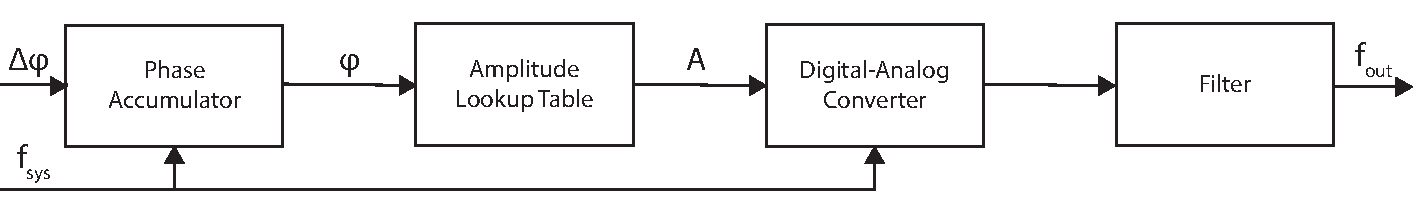
\includegraphics[width=\textwidth]
  {../figure/digital-signal-synthesis/simple-architecture.pdf}
  \caption{Signal flow through a simple \gls{dds}. The output frequency
    determines a phase step by which the accumulator is incremented at each
    clock cycle. The value of the phase accumulator is used for amplitude
    lookup of the desired output signal shape. A \gls{dac} outputs the signal
    which then is filtered to smooth the discrete \gls{dac} output.
  }\label{fig:dds_simple_architecture}
\end{figure}
For every clock cycle the phase accumulator is incremented by $\Delta\varphi$.
On overflow of the accumulator a new signal period starts. The phase
accumulator value is used to lookup the corresponding amplitude value of the
desired output signal shape. For example one can use a lookup table with the
values of a sinusoidal output signal. Alternatively one can omit the lookup
table and output a sawtooth output signal by suppling the phase accumulator
output directly to the \gls{dac} or a square wave signal output by suppling
the most significant bit directly. Finally a \gls{dac} converts the digital
amplitude value to an analog signal. An optional analog filter can be used to
smooth the discrete output. In \Cref{fig:dds_simple_output} the signal at the
different processing stages inside a simple \gls{dds} are presented for a
\SI{8}{\bit} precision, system clock frequency
$f_\text{sys}=\SI{1}{\giga\hertz}$ and output frequency
$f_\text{out}=\SI{100}{\mega\hertz}$.
\begin{figure}[htb]
  \centering
  \begin{adjustbox}{width=\textwidth}
    %% Creator: Matplotlib, PGF backend
%%
%% To include the figure in your LaTeX document, write
%%   \input{<filename>.pgf}
%%
%% Make sure the required packages are loaded in your preamble
%%   \usepackage{pgf}
%%
%% Figures using additional raster images can only be included by \input if
%% they are in the same directory as the main LaTeX file. For loading figures
%% from other directories you can use the `import` package
%%   \usepackage{import}
%% and then include the figures with
%%   \import{<path to file>}{<filename>.pgf}
%%
%% Matplotlib used the following preamble
%%   \usepackage{amsmath}\usepackage{siunitx}\usepackage{lmodern}
%%   \usepackage{fontspec}
%%
\begingroup%
\makeatletter%
\begin{pgfpicture}%
\pgfpathrectangle{\pgfpointorigin}{\pgfqpoint{12.000000in}{8.000000in}}%
\pgfusepath{use as bounding box, clip}%
\begin{pgfscope}%
\pgfsetbuttcap%
\pgfsetmiterjoin%
\pgfsetlinewidth{0.000000pt}%
\definecolor{currentstroke}{rgb}{1.000000,1.000000,1.000000}%
\pgfsetstrokecolor{currentstroke}%
\pgfsetdash{}{0pt}%
\pgfpathmoveto{\pgfqpoint{0.000000in}{0.000000in}}%
\pgfpathlineto{\pgfqpoint{12.000000in}{0.000000in}}%
\pgfpathlineto{\pgfqpoint{12.000000in}{8.000000in}}%
\pgfpathlineto{\pgfqpoint{0.000000in}{8.000000in}}%
\pgfpathclose%
\pgfusepath{}%
\end{pgfscope}%
\begin{pgfscope}%
\pgfsetbuttcap%
\pgfsetmiterjoin%
\definecolor{currentfill}{rgb}{1.000000,1.000000,1.000000}%
\pgfsetfillcolor{currentfill}%
\pgfsetlinewidth{0.000000pt}%
\definecolor{currentstroke}{rgb}{0.000000,0.000000,0.000000}%
\pgfsetstrokecolor{currentstroke}%
\pgfsetstrokeopacity{0.000000}%
\pgfsetdash{}{0pt}%
\pgfpathmoveto{\pgfqpoint{1.500000in}{6.165581in}}%
\pgfpathlineto{\pgfqpoint{10.800000in}{6.165581in}}%
\pgfpathlineto{\pgfqpoint{10.800000in}{7.840000in}}%
\pgfpathlineto{\pgfqpoint{1.500000in}{7.840000in}}%
\pgfpathclose%
\pgfusepath{fill}%
\end{pgfscope}%
\begin{pgfscope}%
\pgfpathrectangle{\pgfqpoint{1.500000in}{6.165581in}}{\pgfqpoint{9.300000in}{1.674419in}}%
\pgfusepath{clip}%
\pgfsetbuttcap%
\pgfsetroundjoin%
\definecolor{currentfill}{rgb}{0.121569,0.466667,0.705882}%
\pgfsetfillcolor{currentfill}%
\pgfsetlinewidth{1.003750pt}%
\definecolor{currentstroke}{rgb}{0.121569,0.466667,0.705882}%
\pgfsetstrokecolor{currentstroke}%
\pgfsetdash{}{0pt}%
\pgfpathmoveto{\pgfqpoint{1.950324in}{6.350153in}}%
\pgfpathcurveto{\pgfqpoint{1.957691in}{6.350153in}}{\pgfqpoint{1.964757in}{6.353079in}}{\pgfqpoint{1.969966in}{6.358289in}}%
\pgfpathcurveto{\pgfqpoint{1.975175in}{6.363498in}}{\pgfqpoint{1.978102in}{6.370564in}}{\pgfqpoint{1.978102in}{6.377930in}}%
\pgfpathcurveto{\pgfqpoint{1.978102in}{6.385297in}}{\pgfqpoint{1.975175in}{6.392363in}}{\pgfqpoint{1.969966in}{6.397572in}}%
\pgfpathcurveto{\pgfqpoint{1.964757in}{6.402781in}}{\pgfqpoint{1.957691in}{6.405708in}}{\pgfqpoint{1.950324in}{6.405708in}}%
\pgfpathcurveto{\pgfqpoint{1.942958in}{6.405708in}}{\pgfqpoint{1.935892in}{6.402781in}}{\pgfqpoint{1.930682in}{6.397572in}}%
\pgfpathcurveto{\pgfqpoint{1.925473in}{6.392363in}}{\pgfqpoint{1.922547in}{6.385297in}}{\pgfqpoint{1.922547in}{6.377930in}}%
\pgfpathcurveto{\pgfqpoint{1.922547in}{6.370564in}}{\pgfqpoint{1.925473in}{6.363498in}}{\pgfqpoint{1.930682in}{6.358289in}}%
\pgfpathcurveto{\pgfqpoint{1.935892in}{6.353079in}}{\pgfqpoint{1.942958in}{6.350153in}}{\pgfqpoint{1.950324in}{6.350153in}}%
\pgfpathclose%
\pgfusepath{stroke,fill}%
\end{pgfscope}%
\begin{pgfscope}%
\pgfpathrectangle{\pgfqpoint{1.500000in}{6.165581in}}{\pgfqpoint{9.300000in}{1.674419in}}%
\pgfusepath{clip}%
\pgfsetbuttcap%
\pgfsetroundjoin%
\definecolor{currentfill}{rgb}{0.121569,0.466667,0.705882}%
\pgfsetfillcolor{currentfill}%
\pgfsetlinewidth{1.003750pt}%
\definecolor{currentstroke}{rgb}{0.121569,0.466667,0.705882}%
\pgfsetstrokecolor{currentstroke}%
\pgfsetdash{}{0pt}%
\pgfpathmoveto{\pgfqpoint{2.121740in}{6.511008in}}%
\pgfpathcurveto{\pgfqpoint{2.129106in}{6.511008in}}{\pgfqpoint{2.136172in}{6.513935in}}{\pgfqpoint{2.141382in}{6.519144in}}%
\pgfpathcurveto{\pgfqpoint{2.146591in}{6.524353in}}{\pgfqpoint{2.149517in}{6.531419in}}{\pgfqpoint{2.149517in}{6.538786in}}%
\pgfpathcurveto{\pgfqpoint{2.149517in}{6.546152in}}{\pgfqpoint{2.146591in}{6.553218in}}{\pgfqpoint{2.141382in}{6.558427in}}%
\pgfpathcurveto{\pgfqpoint{2.136172in}{6.563636in}}{\pgfqpoint{2.129106in}{6.566563in}}{\pgfqpoint{2.121740in}{6.566563in}}%
\pgfpathcurveto{\pgfqpoint{2.114373in}{6.566563in}}{\pgfqpoint{2.107307in}{6.563636in}}{\pgfqpoint{2.102098in}{6.558427in}}%
\pgfpathcurveto{\pgfqpoint{2.096889in}{6.553218in}}{\pgfqpoint{2.093962in}{6.546152in}}{\pgfqpoint{2.093962in}{6.538786in}}%
\pgfpathcurveto{\pgfqpoint{2.093962in}{6.531419in}}{\pgfqpoint{2.096889in}{6.524353in}}{\pgfqpoint{2.102098in}{6.519144in}}%
\pgfpathcurveto{\pgfqpoint{2.107307in}{6.513935in}}{\pgfqpoint{2.114373in}{6.511008in}}{\pgfqpoint{2.121740in}{6.511008in}}%
\pgfpathclose%
\pgfusepath{stroke,fill}%
\end{pgfscope}%
\begin{pgfscope}%
\pgfpathrectangle{\pgfqpoint{1.500000in}{6.165581in}}{\pgfqpoint{9.300000in}{1.674419in}}%
\pgfusepath{clip}%
\pgfsetbuttcap%
\pgfsetroundjoin%
\definecolor{currentfill}{rgb}{0.121569,0.466667,0.705882}%
\pgfsetfillcolor{currentfill}%
\pgfsetlinewidth{1.003750pt}%
\definecolor{currentstroke}{rgb}{0.121569,0.466667,0.705882}%
\pgfsetstrokecolor{currentstroke}%
\pgfsetdash{}{0pt}%
\pgfpathmoveto{\pgfqpoint{2.293155in}{6.671863in}}%
\pgfpathcurveto{\pgfqpoint{2.300522in}{6.671863in}}{\pgfqpoint{2.307588in}{6.674790in}}{\pgfqpoint{2.312797in}{6.679999in}}%
\pgfpathcurveto{\pgfqpoint{2.318006in}{6.685208in}}{\pgfqpoint{2.320933in}{6.692274in}}{\pgfqpoint{2.320933in}{6.699641in}}%
\pgfpathcurveto{\pgfqpoint{2.320933in}{6.707007in}}{\pgfqpoint{2.318006in}{6.714073in}}{\pgfqpoint{2.312797in}{6.719283in}}%
\pgfpathcurveto{\pgfqpoint{2.307588in}{6.724492in}}{\pgfqpoint{2.300522in}{6.727418in}}{\pgfqpoint{2.293155in}{6.727418in}}%
\pgfpathcurveto{\pgfqpoint{2.285788in}{6.727418in}}{\pgfqpoint{2.278722in}{6.724492in}}{\pgfqpoint{2.273513in}{6.719283in}}%
\pgfpathcurveto{\pgfqpoint{2.268304in}{6.714073in}}{\pgfqpoint{2.265377in}{6.707007in}}{\pgfqpoint{2.265377in}{6.699641in}}%
\pgfpathcurveto{\pgfqpoint{2.265377in}{6.692274in}}{\pgfqpoint{2.268304in}{6.685208in}}{\pgfqpoint{2.273513in}{6.679999in}}%
\pgfpathcurveto{\pgfqpoint{2.278722in}{6.674790in}}{\pgfqpoint{2.285788in}{6.671863in}}{\pgfqpoint{2.293155in}{6.671863in}}%
\pgfpathclose%
\pgfusepath{stroke,fill}%
\end{pgfscope}%
\begin{pgfscope}%
\pgfpathrectangle{\pgfqpoint{1.500000in}{6.165581in}}{\pgfqpoint{9.300000in}{1.674419in}}%
\pgfusepath{clip}%
\pgfsetbuttcap%
\pgfsetroundjoin%
\definecolor{currentfill}{rgb}{0.121569,0.466667,0.705882}%
\pgfsetfillcolor{currentfill}%
\pgfsetlinewidth{1.003750pt}%
\definecolor{currentstroke}{rgb}{0.121569,0.466667,0.705882}%
\pgfsetstrokecolor{currentstroke}%
\pgfsetdash{}{0pt}%
\pgfpathmoveto{\pgfqpoint{2.464570in}{6.832718in}}%
\pgfpathcurveto{\pgfqpoint{2.471937in}{6.832718in}}{\pgfqpoint{2.479003in}{6.835645in}}{\pgfqpoint{2.484212in}{6.840854in}}%
\pgfpathcurveto{\pgfqpoint{2.489421in}{6.846063in}}{\pgfqpoint{2.492348in}{6.853129in}}{\pgfqpoint{2.492348in}{6.860496in}}%
\pgfpathcurveto{\pgfqpoint{2.492348in}{6.867863in}}{\pgfqpoint{2.489421in}{6.874929in}}{\pgfqpoint{2.484212in}{6.880138in}}%
\pgfpathcurveto{\pgfqpoint{2.479003in}{6.885347in}}{\pgfqpoint{2.471937in}{6.888274in}}{\pgfqpoint{2.464570in}{6.888274in}}%
\pgfpathcurveto{\pgfqpoint{2.457204in}{6.888274in}}{\pgfqpoint{2.450138in}{6.885347in}}{\pgfqpoint{2.444928in}{6.880138in}}%
\pgfpathcurveto{\pgfqpoint{2.439719in}{6.874929in}}{\pgfqpoint{2.436793in}{6.867863in}}{\pgfqpoint{2.436793in}{6.860496in}}%
\pgfpathcurveto{\pgfqpoint{2.436793in}{6.853129in}}{\pgfqpoint{2.439719in}{6.846063in}}{\pgfqpoint{2.444928in}{6.840854in}}%
\pgfpathcurveto{\pgfqpoint{2.450138in}{6.835645in}}{\pgfqpoint{2.457204in}{6.832718in}}{\pgfqpoint{2.464570in}{6.832718in}}%
\pgfpathclose%
\pgfusepath{stroke,fill}%
\end{pgfscope}%
\begin{pgfscope}%
\pgfpathrectangle{\pgfqpoint{1.500000in}{6.165581in}}{\pgfqpoint{9.300000in}{1.674419in}}%
\pgfusepath{clip}%
\pgfsetbuttcap%
\pgfsetroundjoin%
\definecolor{currentfill}{rgb}{0.121569,0.466667,0.705882}%
\pgfsetfillcolor{currentfill}%
\pgfsetlinewidth{1.003750pt}%
\definecolor{currentstroke}{rgb}{0.121569,0.466667,0.705882}%
\pgfsetstrokecolor{currentstroke}%
\pgfsetdash{}{0pt}%
\pgfpathmoveto{\pgfqpoint{2.635986in}{6.993573in}}%
\pgfpathcurveto{\pgfqpoint{2.643352in}{6.993573in}}{\pgfqpoint{2.650418in}{6.996500in}}{\pgfqpoint{2.655628in}{7.001709in}}%
\pgfpathcurveto{\pgfqpoint{2.660837in}{7.006918in}}{\pgfqpoint{2.663763in}{7.013984in}}{\pgfqpoint{2.663763in}{7.021351in}}%
\pgfpathcurveto{\pgfqpoint{2.663763in}{7.028718in}}{\pgfqpoint{2.660837in}{7.035784in}}{\pgfqpoint{2.655628in}{7.040993in}}%
\pgfpathcurveto{\pgfqpoint{2.650418in}{7.046202in}}{\pgfqpoint{2.643352in}{7.049129in}}{\pgfqpoint{2.635986in}{7.049129in}}%
\pgfpathcurveto{\pgfqpoint{2.628619in}{7.049129in}}{\pgfqpoint{2.621553in}{7.046202in}}{\pgfqpoint{2.616344in}{7.040993in}}%
\pgfpathcurveto{\pgfqpoint{2.611135in}{7.035784in}}{\pgfqpoint{2.608208in}{7.028718in}}{\pgfqpoint{2.608208in}{7.021351in}}%
\pgfpathcurveto{\pgfqpoint{2.608208in}{7.013984in}}{\pgfqpoint{2.611135in}{7.006918in}}{\pgfqpoint{2.616344in}{7.001709in}}%
\pgfpathcurveto{\pgfqpoint{2.621553in}{6.996500in}}{\pgfqpoint{2.628619in}{6.993573in}}{\pgfqpoint{2.635986in}{6.993573in}}%
\pgfpathclose%
\pgfusepath{stroke,fill}%
\end{pgfscope}%
\begin{pgfscope}%
\pgfpathrectangle{\pgfqpoint{1.500000in}{6.165581in}}{\pgfqpoint{9.300000in}{1.674419in}}%
\pgfusepath{clip}%
\pgfsetbuttcap%
\pgfsetroundjoin%
\definecolor{currentfill}{rgb}{0.121569,0.466667,0.705882}%
\pgfsetfillcolor{currentfill}%
\pgfsetlinewidth{1.003750pt}%
\definecolor{currentstroke}{rgb}{0.121569,0.466667,0.705882}%
\pgfsetstrokecolor{currentstroke}%
\pgfsetdash{}{0pt}%
\pgfpathmoveto{\pgfqpoint{2.807401in}{7.154428in}}%
\pgfpathcurveto{\pgfqpoint{2.814768in}{7.154428in}}{\pgfqpoint{2.821834in}{7.157355in}}{\pgfqpoint{2.827043in}{7.162564in}}%
\pgfpathcurveto{\pgfqpoint{2.832252in}{7.167773in}}{\pgfqpoint{2.835179in}{7.174839in}}{\pgfqpoint{2.835179in}{7.182206in}}%
\pgfpathcurveto{\pgfqpoint{2.835179in}{7.189573in}}{\pgfqpoint{2.832252in}{7.196639in}}{\pgfqpoint{2.827043in}{7.201848in}}%
\pgfpathcurveto{\pgfqpoint{2.821834in}{7.207057in}}{\pgfqpoint{2.814768in}{7.209984in}}{\pgfqpoint{2.807401in}{7.209984in}}%
\pgfpathcurveto{\pgfqpoint{2.800034in}{7.209984in}}{\pgfqpoint{2.792968in}{7.207057in}}{\pgfqpoint{2.787759in}{7.201848in}}%
\pgfpathcurveto{\pgfqpoint{2.782550in}{7.196639in}}{\pgfqpoint{2.779623in}{7.189573in}}{\pgfqpoint{2.779623in}{7.182206in}}%
\pgfpathcurveto{\pgfqpoint{2.779623in}{7.174839in}}{\pgfqpoint{2.782550in}{7.167773in}}{\pgfqpoint{2.787759in}{7.162564in}}%
\pgfpathcurveto{\pgfqpoint{2.792968in}{7.157355in}}{\pgfqpoint{2.800034in}{7.154428in}}{\pgfqpoint{2.807401in}{7.154428in}}%
\pgfpathclose%
\pgfusepath{stroke,fill}%
\end{pgfscope}%
\begin{pgfscope}%
\pgfpathrectangle{\pgfqpoint{1.500000in}{6.165581in}}{\pgfqpoint{9.300000in}{1.674419in}}%
\pgfusepath{clip}%
\pgfsetbuttcap%
\pgfsetroundjoin%
\definecolor{currentfill}{rgb}{0.121569,0.466667,0.705882}%
\pgfsetfillcolor{currentfill}%
\pgfsetlinewidth{1.003750pt}%
\definecolor{currentstroke}{rgb}{0.121569,0.466667,0.705882}%
\pgfsetstrokecolor{currentstroke}%
\pgfsetdash{}{0pt}%
\pgfpathmoveto{\pgfqpoint{2.978816in}{7.315283in}}%
\pgfpathcurveto{\pgfqpoint{2.986183in}{7.315283in}}{\pgfqpoint{2.993249in}{7.318210in}}{\pgfqpoint{2.998458in}{7.323419in}}%
\pgfpathcurveto{\pgfqpoint{3.003667in}{7.328628in}}{\pgfqpoint{3.006594in}{7.335694in}}{\pgfqpoint{3.006594in}{7.343061in}}%
\pgfpathcurveto{\pgfqpoint{3.006594in}{7.350428in}}{\pgfqpoint{3.003667in}{7.357494in}}{\pgfqpoint{2.998458in}{7.362703in}}%
\pgfpathcurveto{\pgfqpoint{2.993249in}{7.367912in}}{\pgfqpoint{2.986183in}{7.370839in}}{\pgfqpoint{2.978816in}{7.370839in}}%
\pgfpathcurveto{\pgfqpoint{2.971450in}{7.370839in}}{\pgfqpoint{2.964384in}{7.367912in}}{\pgfqpoint{2.959174in}{7.362703in}}%
\pgfpathcurveto{\pgfqpoint{2.953965in}{7.357494in}}{\pgfqpoint{2.951039in}{7.350428in}}{\pgfqpoint{2.951039in}{7.343061in}}%
\pgfpathcurveto{\pgfqpoint{2.951039in}{7.335694in}}{\pgfqpoint{2.953965in}{7.328628in}}{\pgfqpoint{2.959174in}{7.323419in}}%
\pgfpathcurveto{\pgfqpoint{2.964384in}{7.318210in}}{\pgfqpoint{2.971450in}{7.315283in}}{\pgfqpoint{2.978816in}{7.315283in}}%
\pgfpathclose%
\pgfusepath{stroke,fill}%
\end{pgfscope}%
\begin{pgfscope}%
\pgfpathrectangle{\pgfqpoint{1.500000in}{6.165581in}}{\pgfqpoint{9.300000in}{1.674419in}}%
\pgfusepath{clip}%
\pgfsetbuttcap%
\pgfsetroundjoin%
\definecolor{currentfill}{rgb}{0.121569,0.466667,0.705882}%
\pgfsetfillcolor{currentfill}%
\pgfsetlinewidth{1.003750pt}%
\definecolor{currentstroke}{rgb}{0.121569,0.466667,0.705882}%
\pgfsetstrokecolor{currentstroke}%
\pgfsetdash{}{0pt}%
\pgfpathmoveto{\pgfqpoint{3.150232in}{7.476139in}}%
\pgfpathcurveto{\pgfqpoint{3.157598in}{7.476139in}}{\pgfqpoint{3.164664in}{7.479065in}}{\pgfqpoint{3.169874in}{7.484274in}}%
\pgfpathcurveto{\pgfqpoint{3.175083in}{7.489484in}}{\pgfqpoint{3.178009in}{7.496550in}}{\pgfqpoint{3.178009in}{7.503916in}}%
\pgfpathcurveto{\pgfqpoint{3.178009in}{7.511283in}}{\pgfqpoint{3.175083in}{7.518349in}}{\pgfqpoint{3.169874in}{7.523558in}}%
\pgfpathcurveto{\pgfqpoint{3.164664in}{7.528767in}}{\pgfqpoint{3.157598in}{7.531694in}}{\pgfqpoint{3.150232in}{7.531694in}}%
\pgfpathcurveto{\pgfqpoint{3.142865in}{7.531694in}}{\pgfqpoint{3.135799in}{7.528767in}}{\pgfqpoint{3.130590in}{7.523558in}}%
\pgfpathcurveto{\pgfqpoint{3.125381in}{7.518349in}}{\pgfqpoint{3.122454in}{7.511283in}}{\pgfqpoint{3.122454in}{7.503916in}}%
\pgfpathcurveto{\pgfqpoint{3.122454in}{7.496550in}}{\pgfqpoint{3.125381in}{7.489484in}}{\pgfqpoint{3.130590in}{7.484274in}}%
\pgfpathcurveto{\pgfqpoint{3.135799in}{7.479065in}}{\pgfqpoint{3.142865in}{7.476139in}}{\pgfqpoint{3.150232in}{7.476139in}}%
\pgfpathclose%
\pgfusepath{stroke,fill}%
\end{pgfscope}%
\begin{pgfscope}%
\pgfpathrectangle{\pgfqpoint{1.500000in}{6.165581in}}{\pgfqpoint{9.300000in}{1.674419in}}%
\pgfusepath{clip}%
\pgfsetbuttcap%
\pgfsetroundjoin%
\definecolor{currentfill}{rgb}{0.121569,0.466667,0.705882}%
\pgfsetfillcolor{currentfill}%
\pgfsetlinewidth{1.003750pt}%
\definecolor{currentstroke}{rgb}{0.121569,0.466667,0.705882}%
\pgfsetstrokecolor{currentstroke}%
\pgfsetdash{}{0pt}%
\pgfpathmoveto{\pgfqpoint{3.321647in}{7.636994in}}%
\pgfpathcurveto{\pgfqpoint{3.329014in}{7.636994in}}{\pgfqpoint{3.336080in}{7.639920in}}{\pgfqpoint{3.341289in}{7.645130in}}%
\pgfpathcurveto{\pgfqpoint{3.346498in}{7.650339in}}{\pgfqpoint{3.349425in}{7.657405in}}{\pgfqpoint{3.349425in}{7.664771in}}%
\pgfpathcurveto{\pgfqpoint{3.349425in}{7.672138in}}{\pgfqpoint{3.346498in}{7.679204in}}{\pgfqpoint{3.341289in}{7.684413in}}%
\pgfpathcurveto{\pgfqpoint{3.336080in}{7.689622in}}{\pgfqpoint{3.329014in}{7.692549in}}{\pgfqpoint{3.321647in}{7.692549in}}%
\pgfpathcurveto{\pgfqpoint{3.314280in}{7.692549in}}{\pgfqpoint{3.307214in}{7.689622in}}{\pgfqpoint{3.302005in}{7.684413in}}%
\pgfpathcurveto{\pgfqpoint{3.296796in}{7.679204in}}{\pgfqpoint{3.293869in}{7.672138in}}{\pgfqpoint{3.293869in}{7.664771in}}%
\pgfpathcurveto{\pgfqpoint{3.293869in}{7.657405in}}{\pgfqpoint{3.296796in}{7.650339in}}{\pgfqpoint{3.302005in}{7.645130in}}%
\pgfpathcurveto{\pgfqpoint{3.307214in}{7.639920in}}{\pgfqpoint{3.314280in}{7.636994in}}{\pgfqpoint{3.321647in}{7.636994in}}%
\pgfpathclose%
\pgfusepath{stroke,fill}%
\end{pgfscope}%
\begin{pgfscope}%
\pgfpathrectangle{\pgfqpoint{1.500000in}{6.165581in}}{\pgfqpoint{9.300000in}{1.674419in}}%
\pgfusepath{clip}%
\pgfsetbuttcap%
\pgfsetroundjoin%
\definecolor{currentfill}{rgb}{0.121569,0.466667,0.705882}%
\pgfsetfillcolor{currentfill}%
\pgfsetlinewidth{1.003750pt}%
\definecolor{currentstroke}{rgb}{0.121569,0.466667,0.705882}%
\pgfsetstrokecolor{currentstroke}%
\pgfsetdash{}{0pt}%
\pgfpathmoveto{\pgfqpoint{3.493062in}{6.214044in}}%
\pgfpathcurveto{\pgfqpoint{3.500429in}{6.214044in}}{\pgfqpoint{3.507495in}{6.216971in}}{\pgfqpoint{3.512704in}{6.222180in}}%
\pgfpathcurveto{\pgfqpoint{3.517913in}{6.227389in}}{\pgfqpoint{3.520840in}{6.234455in}}{\pgfqpoint{3.520840in}{6.241822in}}%
\pgfpathcurveto{\pgfqpoint{3.520840in}{6.249189in}}{\pgfqpoint{3.517913in}{6.256255in}}{\pgfqpoint{3.512704in}{6.261464in}}%
\pgfpathcurveto{\pgfqpoint{3.507495in}{6.266673in}}{\pgfqpoint{3.500429in}{6.269600in}}{\pgfqpoint{3.493062in}{6.269600in}}%
\pgfpathcurveto{\pgfqpoint{3.485696in}{6.269600in}}{\pgfqpoint{3.478630in}{6.266673in}}{\pgfqpoint{3.473420in}{6.261464in}}%
\pgfpathcurveto{\pgfqpoint{3.468211in}{6.256255in}}{\pgfqpoint{3.465285in}{6.249189in}}{\pgfqpoint{3.465285in}{6.241822in}}%
\pgfpathcurveto{\pgfqpoint{3.465285in}{6.234455in}}{\pgfqpoint{3.468211in}{6.227389in}}{\pgfqpoint{3.473420in}{6.222180in}}%
\pgfpathcurveto{\pgfqpoint{3.478630in}{6.216971in}}{\pgfqpoint{3.485696in}{6.214044in}}{\pgfqpoint{3.493062in}{6.214044in}}%
\pgfpathclose%
\pgfusepath{stroke,fill}%
\end{pgfscope}%
\begin{pgfscope}%
\pgfpathrectangle{\pgfqpoint{1.500000in}{6.165581in}}{\pgfqpoint{9.300000in}{1.674419in}}%
\pgfusepath{clip}%
\pgfsetbuttcap%
\pgfsetroundjoin%
\definecolor{currentfill}{rgb}{0.121569,0.466667,0.705882}%
\pgfsetfillcolor{currentfill}%
\pgfsetlinewidth{1.003750pt}%
\definecolor{currentstroke}{rgb}{0.121569,0.466667,0.705882}%
\pgfsetstrokecolor{currentstroke}%
\pgfsetdash{}{0pt}%
\pgfpathmoveto{\pgfqpoint{3.664478in}{6.374900in}}%
\pgfpathcurveto{\pgfqpoint{3.671844in}{6.374900in}}{\pgfqpoint{3.678910in}{6.377826in}}{\pgfqpoint{3.684120in}{6.383035in}}%
\pgfpathcurveto{\pgfqpoint{3.689329in}{6.388245in}}{\pgfqpoint{3.692255in}{6.395311in}}{\pgfqpoint{3.692255in}{6.402677in}}%
\pgfpathcurveto{\pgfqpoint{3.692255in}{6.410044in}}{\pgfqpoint{3.689329in}{6.417110in}}{\pgfqpoint{3.684120in}{6.422319in}}%
\pgfpathcurveto{\pgfqpoint{3.678910in}{6.427528in}}{\pgfqpoint{3.671844in}{6.430455in}}{\pgfqpoint{3.664478in}{6.430455in}}%
\pgfpathcurveto{\pgfqpoint{3.657111in}{6.430455in}}{\pgfqpoint{3.650045in}{6.427528in}}{\pgfqpoint{3.644836in}{6.422319in}}%
\pgfpathcurveto{\pgfqpoint{3.639627in}{6.417110in}}{\pgfqpoint{3.636700in}{6.410044in}}{\pgfqpoint{3.636700in}{6.402677in}}%
\pgfpathcurveto{\pgfqpoint{3.636700in}{6.395311in}}{\pgfqpoint{3.639627in}{6.388245in}}{\pgfqpoint{3.644836in}{6.383035in}}%
\pgfpathcurveto{\pgfqpoint{3.650045in}{6.377826in}}{\pgfqpoint{3.657111in}{6.374900in}}{\pgfqpoint{3.664478in}{6.374900in}}%
\pgfpathclose%
\pgfusepath{stroke,fill}%
\end{pgfscope}%
\begin{pgfscope}%
\pgfpathrectangle{\pgfqpoint{1.500000in}{6.165581in}}{\pgfqpoint{9.300000in}{1.674419in}}%
\pgfusepath{clip}%
\pgfsetbuttcap%
\pgfsetroundjoin%
\definecolor{currentfill}{rgb}{0.121569,0.466667,0.705882}%
\pgfsetfillcolor{currentfill}%
\pgfsetlinewidth{1.003750pt}%
\definecolor{currentstroke}{rgb}{0.121569,0.466667,0.705882}%
\pgfsetstrokecolor{currentstroke}%
\pgfsetdash{}{0pt}%
\pgfpathmoveto{\pgfqpoint{3.835893in}{6.535755in}}%
\pgfpathcurveto{\pgfqpoint{3.843260in}{6.535755in}}{\pgfqpoint{3.850326in}{6.538682in}}{\pgfqpoint{3.855535in}{6.543891in}}%
\pgfpathcurveto{\pgfqpoint{3.860744in}{6.549100in}}{\pgfqpoint{3.863671in}{6.556166in}}{\pgfqpoint{3.863671in}{6.563532in}}%
\pgfpathcurveto{\pgfqpoint{3.863671in}{6.570899in}}{\pgfqpoint{3.860744in}{6.577965in}}{\pgfqpoint{3.855535in}{6.583174in}}%
\pgfpathcurveto{\pgfqpoint{3.850326in}{6.588383in}}{\pgfqpoint{3.843260in}{6.591310in}}{\pgfqpoint{3.835893in}{6.591310in}}%
\pgfpathcurveto{\pgfqpoint{3.828526in}{6.591310in}}{\pgfqpoint{3.821460in}{6.588383in}}{\pgfqpoint{3.816251in}{6.583174in}}%
\pgfpathcurveto{\pgfqpoint{3.811042in}{6.577965in}}{\pgfqpoint{3.808115in}{6.570899in}}{\pgfqpoint{3.808115in}{6.563532in}}%
\pgfpathcurveto{\pgfqpoint{3.808115in}{6.556166in}}{\pgfqpoint{3.811042in}{6.549100in}}{\pgfqpoint{3.816251in}{6.543891in}}%
\pgfpathcurveto{\pgfqpoint{3.821460in}{6.538682in}}{\pgfqpoint{3.828526in}{6.535755in}}{\pgfqpoint{3.835893in}{6.535755in}}%
\pgfpathclose%
\pgfusepath{stroke,fill}%
\end{pgfscope}%
\begin{pgfscope}%
\pgfpathrectangle{\pgfqpoint{1.500000in}{6.165581in}}{\pgfqpoint{9.300000in}{1.674419in}}%
\pgfusepath{clip}%
\pgfsetbuttcap%
\pgfsetroundjoin%
\definecolor{currentfill}{rgb}{0.121569,0.466667,0.705882}%
\pgfsetfillcolor{currentfill}%
\pgfsetlinewidth{1.003750pt}%
\definecolor{currentstroke}{rgb}{0.121569,0.466667,0.705882}%
\pgfsetstrokecolor{currentstroke}%
\pgfsetdash{}{0pt}%
\pgfpathmoveto{\pgfqpoint{4.007308in}{6.696610in}}%
\pgfpathcurveto{\pgfqpoint{4.014675in}{6.696610in}}{\pgfqpoint{4.021741in}{6.699537in}}{\pgfqpoint{4.026950in}{6.704746in}}%
\pgfpathcurveto{\pgfqpoint{4.032159in}{6.709955in}}{\pgfqpoint{4.035086in}{6.717021in}}{\pgfqpoint{4.035086in}{6.724388in}}%
\pgfpathcurveto{\pgfqpoint{4.035086in}{6.731754in}}{\pgfqpoint{4.032159in}{6.738820in}}{\pgfqpoint{4.026950in}{6.744029in}}%
\pgfpathcurveto{\pgfqpoint{4.021741in}{6.749239in}}{\pgfqpoint{4.014675in}{6.752165in}}{\pgfqpoint{4.007308in}{6.752165in}}%
\pgfpathcurveto{\pgfqpoint{3.999942in}{6.752165in}}{\pgfqpoint{3.992876in}{6.749239in}}{\pgfqpoint{3.987666in}{6.744029in}}%
\pgfpathcurveto{\pgfqpoint{3.982457in}{6.738820in}}{\pgfqpoint{3.979531in}{6.731754in}}{\pgfqpoint{3.979531in}{6.724388in}}%
\pgfpathcurveto{\pgfqpoint{3.979531in}{6.717021in}}{\pgfqpoint{3.982457in}{6.709955in}}{\pgfqpoint{3.987666in}{6.704746in}}%
\pgfpathcurveto{\pgfqpoint{3.992876in}{6.699537in}}{\pgfqpoint{3.999942in}{6.696610in}}{\pgfqpoint{4.007308in}{6.696610in}}%
\pgfpathclose%
\pgfusepath{stroke,fill}%
\end{pgfscope}%
\begin{pgfscope}%
\pgfpathrectangle{\pgfqpoint{1.500000in}{6.165581in}}{\pgfqpoint{9.300000in}{1.674419in}}%
\pgfusepath{clip}%
\pgfsetbuttcap%
\pgfsetroundjoin%
\definecolor{currentfill}{rgb}{0.121569,0.466667,0.705882}%
\pgfsetfillcolor{currentfill}%
\pgfsetlinewidth{1.003750pt}%
\definecolor{currentstroke}{rgb}{0.121569,0.466667,0.705882}%
\pgfsetstrokecolor{currentstroke}%
\pgfsetdash{}{0pt}%
\pgfpathmoveto{\pgfqpoint{4.178724in}{6.857465in}}%
\pgfpathcurveto{\pgfqpoint{4.186090in}{6.857465in}}{\pgfqpoint{4.193156in}{6.860392in}}{\pgfqpoint{4.198366in}{6.865601in}}%
\pgfpathcurveto{\pgfqpoint{4.203575in}{6.870810in}}{\pgfqpoint{4.206501in}{6.877876in}}{\pgfqpoint{4.206501in}{6.885243in}}%
\pgfpathcurveto{\pgfqpoint{4.206501in}{6.892609in}}{\pgfqpoint{4.203575in}{6.899675in}}{\pgfqpoint{4.198366in}{6.904885in}}%
\pgfpathcurveto{\pgfqpoint{4.193156in}{6.910094in}}{\pgfqpoint{4.186090in}{6.913020in}}{\pgfqpoint{4.178724in}{6.913020in}}%
\pgfpathcurveto{\pgfqpoint{4.171357in}{6.913020in}}{\pgfqpoint{4.164291in}{6.910094in}}{\pgfqpoint{4.159082in}{6.904885in}}%
\pgfpathcurveto{\pgfqpoint{4.153873in}{6.899675in}}{\pgfqpoint{4.150946in}{6.892609in}}{\pgfqpoint{4.150946in}{6.885243in}}%
\pgfpathcurveto{\pgfqpoint{4.150946in}{6.877876in}}{\pgfqpoint{4.153873in}{6.870810in}}{\pgfqpoint{4.159082in}{6.865601in}}%
\pgfpathcurveto{\pgfqpoint{4.164291in}{6.860392in}}{\pgfqpoint{4.171357in}{6.857465in}}{\pgfqpoint{4.178724in}{6.857465in}}%
\pgfpathclose%
\pgfusepath{stroke,fill}%
\end{pgfscope}%
\begin{pgfscope}%
\pgfpathrectangle{\pgfqpoint{1.500000in}{6.165581in}}{\pgfqpoint{9.300000in}{1.674419in}}%
\pgfusepath{clip}%
\pgfsetbuttcap%
\pgfsetroundjoin%
\definecolor{currentfill}{rgb}{0.121569,0.466667,0.705882}%
\pgfsetfillcolor{currentfill}%
\pgfsetlinewidth{1.003750pt}%
\definecolor{currentstroke}{rgb}{0.121569,0.466667,0.705882}%
\pgfsetstrokecolor{currentstroke}%
\pgfsetdash{}{0pt}%
\pgfpathmoveto{\pgfqpoint{4.350139in}{7.018320in}}%
\pgfpathcurveto{\pgfqpoint{4.357506in}{7.018320in}}{\pgfqpoint{4.364572in}{7.021247in}}{\pgfqpoint{4.369781in}{7.026456in}}%
\pgfpathcurveto{\pgfqpoint{4.374990in}{7.031665in}}{\pgfqpoint{4.377917in}{7.038731in}}{\pgfqpoint{4.377917in}{7.046098in}}%
\pgfpathcurveto{\pgfqpoint{4.377917in}{7.053465in}}{\pgfqpoint{4.374990in}{7.060531in}}{\pgfqpoint{4.369781in}{7.065740in}}%
\pgfpathcurveto{\pgfqpoint{4.364572in}{7.070949in}}{\pgfqpoint{4.357506in}{7.073876in}}{\pgfqpoint{4.350139in}{7.073876in}}%
\pgfpathcurveto{\pgfqpoint{4.342772in}{7.073876in}}{\pgfqpoint{4.335706in}{7.070949in}}{\pgfqpoint{4.330497in}{7.065740in}}%
\pgfpathcurveto{\pgfqpoint{4.325288in}{7.060531in}}{\pgfqpoint{4.322361in}{7.053465in}}{\pgfqpoint{4.322361in}{7.046098in}}%
\pgfpathcurveto{\pgfqpoint{4.322361in}{7.038731in}}{\pgfqpoint{4.325288in}{7.031665in}}{\pgfqpoint{4.330497in}{7.026456in}}%
\pgfpathcurveto{\pgfqpoint{4.335706in}{7.021247in}}{\pgfqpoint{4.342772in}{7.018320in}}{\pgfqpoint{4.350139in}{7.018320in}}%
\pgfpathclose%
\pgfusepath{stroke,fill}%
\end{pgfscope}%
\begin{pgfscope}%
\pgfpathrectangle{\pgfqpoint{1.500000in}{6.165581in}}{\pgfqpoint{9.300000in}{1.674419in}}%
\pgfusepath{clip}%
\pgfsetbuttcap%
\pgfsetroundjoin%
\definecolor{currentfill}{rgb}{0.121569,0.466667,0.705882}%
\pgfsetfillcolor{currentfill}%
\pgfsetlinewidth{1.003750pt}%
\definecolor{currentstroke}{rgb}{0.121569,0.466667,0.705882}%
\pgfsetstrokecolor{currentstroke}%
\pgfsetdash{}{0pt}%
\pgfpathmoveto{\pgfqpoint{4.521554in}{7.179175in}}%
\pgfpathcurveto{\pgfqpoint{4.528921in}{7.179175in}}{\pgfqpoint{4.535987in}{7.182102in}}{\pgfqpoint{4.541196in}{7.187311in}}%
\pgfpathcurveto{\pgfqpoint{4.546405in}{7.192520in}}{\pgfqpoint{4.549332in}{7.199586in}}{\pgfqpoint{4.549332in}{7.206953in}}%
\pgfpathcurveto{\pgfqpoint{4.549332in}{7.214320in}}{\pgfqpoint{4.546405in}{7.221386in}}{\pgfqpoint{4.541196in}{7.226595in}}%
\pgfpathcurveto{\pgfqpoint{4.535987in}{7.231804in}}{\pgfqpoint{4.528921in}{7.234731in}}{\pgfqpoint{4.521554in}{7.234731in}}%
\pgfpathcurveto{\pgfqpoint{4.514188in}{7.234731in}}{\pgfqpoint{4.507122in}{7.231804in}}{\pgfqpoint{4.501912in}{7.226595in}}%
\pgfpathcurveto{\pgfqpoint{4.496703in}{7.221386in}}{\pgfqpoint{4.493777in}{7.214320in}}{\pgfqpoint{4.493777in}{7.206953in}}%
\pgfpathcurveto{\pgfqpoint{4.493777in}{7.199586in}}{\pgfqpoint{4.496703in}{7.192520in}}{\pgfqpoint{4.501912in}{7.187311in}}%
\pgfpathcurveto{\pgfqpoint{4.507122in}{7.182102in}}{\pgfqpoint{4.514188in}{7.179175in}}{\pgfqpoint{4.521554in}{7.179175in}}%
\pgfpathclose%
\pgfusepath{stroke,fill}%
\end{pgfscope}%
\begin{pgfscope}%
\pgfpathrectangle{\pgfqpoint{1.500000in}{6.165581in}}{\pgfqpoint{9.300000in}{1.674419in}}%
\pgfusepath{clip}%
\pgfsetbuttcap%
\pgfsetroundjoin%
\definecolor{currentfill}{rgb}{0.121569,0.466667,0.705882}%
\pgfsetfillcolor{currentfill}%
\pgfsetlinewidth{1.003750pt}%
\definecolor{currentstroke}{rgb}{0.121569,0.466667,0.705882}%
\pgfsetstrokecolor{currentstroke}%
\pgfsetdash{}{0pt}%
\pgfpathmoveto{\pgfqpoint{4.692970in}{7.340030in}}%
\pgfpathcurveto{\pgfqpoint{4.700336in}{7.340030in}}{\pgfqpoint{4.707402in}{7.342957in}}{\pgfqpoint{4.712612in}{7.348166in}}%
\pgfpathcurveto{\pgfqpoint{4.717821in}{7.353375in}}{\pgfqpoint{4.720747in}{7.360441in}}{\pgfqpoint{4.720747in}{7.367808in}}%
\pgfpathcurveto{\pgfqpoint{4.720747in}{7.375175in}}{\pgfqpoint{4.717821in}{7.382241in}}{\pgfqpoint{4.712612in}{7.387450in}}%
\pgfpathcurveto{\pgfqpoint{4.707402in}{7.392659in}}{\pgfqpoint{4.700336in}{7.395586in}}{\pgfqpoint{4.692970in}{7.395586in}}%
\pgfpathcurveto{\pgfqpoint{4.685603in}{7.395586in}}{\pgfqpoint{4.678537in}{7.392659in}}{\pgfqpoint{4.673328in}{7.387450in}}%
\pgfpathcurveto{\pgfqpoint{4.668119in}{7.382241in}}{\pgfqpoint{4.665192in}{7.375175in}}{\pgfqpoint{4.665192in}{7.367808in}}%
\pgfpathcurveto{\pgfqpoint{4.665192in}{7.360441in}}{\pgfqpoint{4.668119in}{7.353375in}}{\pgfqpoint{4.673328in}{7.348166in}}%
\pgfpathcurveto{\pgfqpoint{4.678537in}{7.342957in}}{\pgfqpoint{4.685603in}{7.340030in}}{\pgfqpoint{4.692970in}{7.340030in}}%
\pgfpathclose%
\pgfusepath{stroke,fill}%
\end{pgfscope}%
\begin{pgfscope}%
\pgfpathrectangle{\pgfqpoint{1.500000in}{6.165581in}}{\pgfqpoint{9.300000in}{1.674419in}}%
\pgfusepath{clip}%
\pgfsetbuttcap%
\pgfsetroundjoin%
\definecolor{currentfill}{rgb}{0.121569,0.466667,0.705882}%
\pgfsetfillcolor{currentfill}%
\pgfsetlinewidth{1.003750pt}%
\definecolor{currentstroke}{rgb}{0.121569,0.466667,0.705882}%
\pgfsetstrokecolor{currentstroke}%
\pgfsetdash{}{0pt}%
\pgfpathmoveto{\pgfqpoint{4.864385in}{7.500885in}}%
\pgfpathcurveto{\pgfqpoint{4.871752in}{7.500885in}}{\pgfqpoint{4.878818in}{7.503812in}}{\pgfqpoint{4.884027in}{7.509021in}}%
\pgfpathcurveto{\pgfqpoint{4.889236in}{7.514230in}}{\pgfqpoint{4.892163in}{7.521296in}}{\pgfqpoint{4.892163in}{7.528663in}}%
\pgfpathcurveto{\pgfqpoint{4.892163in}{7.536030in}}{\pgfqpoint{4.889236in}{7.543096in}}{\pgfqpoint{4.884027in}{7.548305in}}%
\pgfpathcurveto{\pgfqpoint{4.878818in}{7.553514in}}{\pgfqpoint{4.871752in}{7.556441in}}{\pgfqpoint{4.864385in}{7.556441in}}%
\pgfpathcurveto{\pgfqpoint{4.857018in}{7.556441in}}{\pgfqpoint{4.849952in}{7.553514in}}{\pgfqpoint{4.844743in}{7.548305in}}%
\pgfpathcurveto{\pgfqpoint{4.839534in}{7.543096in}}{\pgfqpoint{4.836607in}{7.536030in}}{\pgfqpoint{4.836607in}{7.528663in}}%
\pgfpathcurveto{\pgfqpoint{4.836607in}{7.521296in}}{\pgfqpoint{4.839534in}{7.514230in}}{\pgfqpoint{4.844743in}{7.509021in}}%
\pgfpathcurveto{\pgfqpoint{4.849952in}{7.503812in}}{\pgfqpoint{4.857018in}{7.500885in}}{\pgfqpoint{4.864385in}{7.500885in}}%
\pgfpathclose%
\pgfusepath{stroke,fill}%
\end{pgfscope}%
\begin{pgfscope}%
\pgfpathrectangle{\pgfqpoint{1.500000in}{6.165581in}}{\pgfqpoint{9.300000in}{1.674419in}}%
\pgfusepath{clip}%
\pgfsetbuttcap%
\pgfsetroundjoin%
\definecolor{currentfill}{rgb}{0.121569,0.466667,0.705882}%
\pgfsetfillcolor{currentfill}%
\pgfsetlinewidth{1.003750pt}%
\definecolor{currentstroke}{rgb}{0.121569,0.466667,0.705882}%
\pgfsetstrokecolor{currentstroke}%
\pgfsetdash{}{0pt}%
\pgfpathmoveto{\pgfqpoint{5.035800in}{7.661741in}}%
\pgfpathcurveto{\pgfqpoint{5.043167in}{7.661741in}}{\pgfqpoint{5.050233in}{7.664667in}}{\pgfqpoint{5.055442in}{7.669876in}}%
\pgfpathcurveto{\pgfqpoint{5.060651in}{7.675086in}}{\pgfqpoint{5.063578in}{7.682152in}}{\pgfqpoint{5.063578in}{7.689518in}}%
\pgfpathcurveto{\pgfqpoint{5.063578in}{7.696885in}}{\pgfqpoint{5.060651in}{7.703951in}}{\pgfqpoint{5.055442in}{7.709160in}}%
\pgfpathcurveto{\pgfqpoint{5.050233in}{7.714369in}}{\pgfqpoint{5.043167in}{7.717296in}}{\pgfqpoint{5.035800in}{7.717296in}}%
\pgfpathcurveto{\pgfqpoint{5.028434in}{7.717296in}}{\pgfqpoint{5.021368in}{7.714369in}}{\pgfqpoint{5.016158in}{7.709160in}}%
\pgfpathcurveto{\pgfqpoint{5.010949in}{7.703951in}}{\pgfqpoint{5.008023in}{7.696885in}}{\pgfqpoint{5.008023in}{7.689518in}}%
\pgfpathcurveto{\pgfqpoint{5.008023in}{7.682152in}}{\pgfqpoint{5.010949in}{7.675086in}}{\pgfqpoint{5.016158in}{7.669876in}}%
\pgfpathcurveto{\pgfqpoint{5.021368in}{7.664667in}}{\pgfqpoint{5.028434in}{7.661741in}}{\pgfqpoint{5.035800in}{7.661741in}}%
\pgfpathclose%
\pgfusepath{stroke,fill}%
\end{pgfscope}%
\begin{pgfscope}%
\pgfpathrectangle{\pgfqpoint{1.500000in}{6.165581in}}{\pgfqpoint{9.300000in}{1.674419in}}%
\pgfusepath{clip}%
\pgfsetbuttcap%
\pgfsetroundjoin%
\definecolor{currentfill}{rgb}{0.121569,0.466667,0.705882}%
\pgfsetfillcolor{currentfill}%
\pgfsetlinewidth{1.003750pt}%
\definecolor{currentstroke}{rgb}{0.121569,0.466667,0.705882}%
\pgfsetstrokecolor{currentstroke}%
\pgfsetdash{}{0pt}%
\pgfpathmoveto{\pgfqpoint{5.207216in}{6.238791in}}%
\pgfpathcurveto{\pgfqpoint{5.214582in}{6.238791in}}{\pgfqpoint{5.221648in}{6.241718in}}{\pgfqpoint{5.226858in}{6.246927in}}%
\pgfpathcurveto{\pgfqpoint{5.232067in}{6.252136in}}{\pgfqpoint{5.234993in}{6.259202in}}{\pgfqpoint{5.234993in}{6.266569in}}%
\pgfpathcurveto{\pgfqpoint{5.234993in}{6.273936in}}{\pgfqpoint{5.232067in}{6.281002in}}{\pgfqpoint{5.226858in}{6.286211in}}%
\pgfpathcurveto{\pgfqpoint{5.221648in}{6.291420in}}{\pgfqpoint{5.214582in}{6.294347in}}{\pgfqpoint{5.207216in}{6.294347in}}%
\pgfpathcurveto{\pgfqpoint{5.199849in}{6.294347in}}{\pgfqpoint{5.192783in}{6.291420in}}{\pgfqpoint{5.187574in}{6.286211in}}%
\pgfpathcurveto{\pgfqpoint{5.182365in}{6.281002in}}{\pgfqpoint{5.179438in}{6.273936in}}{\pgfqpoint{5.179438in}{6.266569in}}%
\pgfpathcurveto{\pgfqpoint{5.179438in}{6.259202in}}{\pgfqpoint{5.182365in}{6.252136in}}{\pgfqpoint{5.187574in}{6.246927in}}%
\pgfpathcurveto{\pgfqpoint{5.192783in}{6.241718in}}{\pgfqpoint{5.199849in}{6.238791in}}{\pgfqpoint{5.207216in}{6.238791in}}%
\pgfpathclose%
\pgfusepath{stroke,fill}%
\end{pgfscope}%
\begin{pgfscope}%
\pgfpathrectangle{\pgfqpoint{1.500000in}{6.165581in}}{\pgfqpoint{9.300000in}{1.674419in}}%
\pgfusepath{clip}%
\pgfsetbuttcap%
\pgfsetroundjoin%
\definecolor{currentfill}{rgb}{0.121569,0.466667,0.705882}%
\pgfsetfillcolor{currentfill}%
\pgfsetlinewidth{1.003750pt}%
\definecolor{currentstroke}{rgb}{0.121569,0.466667,0.705882}%
\pgfsetstrokecolor{currentstroke}%
\pgfsetdash{}{0pt}%
\pgfpathmoveto{\pgfqpoint{5.378631in}{6.399647in}}%
\pgfpathcurveto{\pgfqpoint{5.385998in}{6.399647in}}{\pgfqpoint{5.393064in}{6.402573in}}{\pgfqpoint{5.398273in}{6.407782in}}%
\pgfpathcurveto{\pgfqpoint{5.403482in}{6.412992in}}{\pgfqpoint{5.406409in}{6.420058in}}{\pgfqpoint{5.406409in}{6.427424in}}%
\pgfpathcurveto{\pgfqpoint{5.406409in}{6.434791in}}{\pgfqpoint{5.403482in}{6.441857in}}{\pgfqpoint{5.398273in}{6.447066in}}%
\pgfpathcurveto{\pgfqpoint{5.393064in}{6.452275in}}{\pgfqpoint{5.385998in}{6.455202in}}{\pgfqpoint{5.378631in}{6.455202in}}%
\pgfpathcurveto{\pgfqpoint{5.371264in}{6.455202in}}{\pgfqpoint{5.364198in}{6.452275in}}{\pgfqpoint{5.358989in}{6.447066in}}%
\pgfpathcurveto{\pgfqpoint{5.353780in}{6.441857in}}{\pgfqpoint{5.350853in}{6.434791in}}{\pgfqpoint{5.350853in}{6.427424in}}%
\pgfpathcurveto{\pgfqpoint{5.350853in}{6.420058in}}{\pgfqpoint{5.353780in}{6.412992in}}{\pgfqpoint{5.358989in}{6.407782in}}%
\pgfpathcurveto{\pgfqpoint{5.364198in}{6.402573in}}{\pgfqpoint{5.371264in}{6.399647in}}{\pgfqpoint{5.378631in}{6.399647in}}%
\pgfpathclose%
\pgfusepath{stroke,fill}%
\end{pgfscope}%
\begin{pgfscope}%
\pgfpathrectangle{\pgfqpoint{1.500000in}{6.165581in}}{\pgfqpoint{9.300000in}{1.674419in}}%
\pgfusepath{clip}%
\pgfsetbuttcap%
\pgfsetroundjoin%
\definecolor{currentfill}{rgb}{0.121569,0.466667,0.705882}%
\pgfsetfillcolor{currentfill}%
\pgfsetlinewidth{1.003750pt}%
\definecolor{currentstroke}{rgb}{0.121569,0.466667,0.705882}%
\pgfsetstrokecolor{currentstroke}%
\pgfsetdash{}{0pt}%
\pgfpathmoveto{\pgfqpoint{5.550046in}{6.560502in}}%
\pgfpathcurveto{\pgfqpoint{5.557413in}{6.560502in}}{\pgfqpoint{5.564479in}{6.563428in}}{\pgfqpoint{5.569688in}{6.568638in}}%
\pgfpathcurveto{\pgfqpoint{5.574897in}{6.573847in}}{\pgfqpoint{5.577824in}{6.580913in}}{\pgfqpoint{5.577824in}{6.588279in}}%
\pgfpathcurveto{\pgfqpoint{5.577824in}{6.595646in}}{\pgfqpoint{5.574897in}{6.602712in}}{\pgfqpoint{5.569688in}{6.607921in}}%
\pgfpathcurveto{\pgfqpoint{5.564479in}{6.613130in}}{\pgfqpoint{5.557413in}{6.616057in}}{\pgfqpoint{5.550046in}{6.616057in}}%
\pgfpathcurveto{\pgfqpoint{5.542680in}{6.616057in}}{\pgfqpoint{5.535614in}{6.613130in}}{\pgfqpoint{5.530404in}{6.607921in}}%
\pgfpathcurveto{\pgfqpoint{5.525195in}{6.602712in}}{\pgfqpoint{5.522269in}{6.595646in}}{\pgfqpoint{5.522269in}{6.588279in}}%
\pgfpathcurveto{\pgfqpoint{5.522269in}{6.580913in}}{\pgfqpoint{5.525195in}{6.573847in}}{\pgfqpoint{5.530404in}{6.568638in}}%
\pgfpathcurveto{\pgfqpoint{5.535614in}{6.563428in}}{\pgfqpoint{5.542680in}{6.560502in}}{\pgfqpoint{5.550046in}{6.560502in}}%
\pgfpathclose%
\pgfusepath{stroke,fill}%
\end{pgfscope}%
\begin{pgfscope}%
\pgfpathrectangle{\pgfqpoint{1.500000in}{6.165581in}}{\pgfqpoint{9.300000in}{1.674419in}}%
\pgfusepath{clip}%
\pgfsetbuttcap%
\pgfsetroundjoin%
\definecolor{currentfill}{rgb}{0.121569,0.466667,0.705882}%
\pgfsetfillcolor{currentfill}%
\pgfsetlinewidth{1.003750pt}%
\definecolor{currentstroke}{rgb}{0.121569,0.466667,0.705882}%
\pgfsetstrokecolor{currentstroke}%
\pgfsetdash{}{0pt}%
\pgfpathmoveto{\pgfqpoint{5.721462in}{6.721357in}}%
\pgfpathcurveto{\pgfqpoint{5.728828in}{6.721357in}}{\pgfqpoint{5.735894in}{6.724284in}}{\pgfqpoint{5.741104in}{6.729493in}}%
\pgfpathcurveto{\pgfqpoint{5.746313in}{6.734702in}}{\pgfqpoint{5.749239in}{6.741768in}}{\pgfqpoint{5.749239in}{6.749135in}}%
\pgfpathcurveto{\pgfqpoint{5.749239in}{6.756501in}}{\pgfqpoint{5.746313in}{6.763567in}}{\pgfqpoint{5.741104in}{6.768776in}}%
\pgfpathcurveto{\pgfqpoint{5.735894in}{6.773985in}}{\pgfqpoint{5.728828in}{6.776912in}}{\pgfqpoint{5.721462in}{6.776912in}}%
\pgfpathcurveto{\pgfqpoint{5.714095in}{6.776912in}}{\pgfqpoint{5.707029in}{6.773985in}}{\pgfqpoint{5.701820in}{6.768776in}}%
\pgfpathcurveto{\pgfqpoint{5.696611in}{6.763567in}}{\pgfqpoint{5.693684in}{6.756501in}}{\pgfqpoint{5.693684in}{6.749135in}}%
\pgfpathcurveto{\pgfqpoint{5.693684in}{6.741768in}}{\pgfqpoint{5.696611in}{6.734702in}}{\pgfqpoint{5.701820in}{6.729493in}}%
\pgfpathcurveto{\pgfqpoint{5.707029in}{6.724284in}}{\pgfqpoint{5.714095in}{6.721357in}}{\pgfqpoint{5.721462in}{6.721357in}}%
\pgfpathclose%
\pgfusepath{stroke,fill}%
\end{pgfscope}%
\begin{pgfscope}%
\pgfpathrectangle{\pgfqpoint{1.500000in}{6.165581in}}{\pgfqpoint{9.300000in}{1.674419in}}%
\pgfusepath{clip}%
\pgfsetbuttcap%
\pgfsetroundjoin%
\definecolor{currentfill}{rgb}{0.121569,0.466667,0.705882}%
\pgfsetfillcolor{currentfill}%
\pgfsetlinewidth{1.003750pt}%
\definecolor{currentstroke}{rgb}{0.121569,0.466667,0.705882}%
\pgfsetstrokecolor{currentstroke}%
\pgfsetdash{}{0pt}%
\pgfpathmoveto{\pgfqpoint{5.892877in}{6.882212in}}%
\pgfpathcurveto{\pgfqpoint{5.900244in}{6.882212in}}{\pgfqpoint{5.907310in}{6.885139in}}{\pgfqpoint{5.912519in}{6.890348in}}%
\pgfpathcurveto{\pgfqpoint{5.917728in}{6.895557in}}{\pgfqpoint{5.920655in}{6.902623in}}{\pgfqpoint{5.920655in}{6.909990in}}%
\pgfpathcurveto{\pgfqpoint{5.920655in}{6.917356in}}{\pgfqpoint{5.917728in}{6.924422in}}{\pgfqpoint{5.912519in}{6.929632in}}%
\pgfpathcurveto{\pgfqpoint{5.907310in}{6.934841in}}{\pgfqpoint{5.900244in}{6.937767in}}{\pgfqpoint{5.892877in}{6.937767in}}%
\pgfpathcurveto{\pgfqpoint{5.885510in}{6.937767in}}{\pgfqpoint{5.878444in}{6.934841in}}{\pgfqpoint{5.873235in}{6.929632in}}%
\pgfpathcurveto{\pgfqpoint{5.868026in}{6.924422in}}{\pgfqpoint{5.865099in}{6.917356in}}{\pgfqpoint{5.865099in}{6.909990in}}%
\pgfpathcurveto{\pgfqpoint{5.865099in}{6.902623in}}{\pgfqpoint{5.868026in}{6.895557in}}{\pgfqpoint{5.873235in}{6.890348in}}%
\pgfpathcurveto{\pgfqpoint{5.878444in}{6.885139in}}{\pgfqpoint{5.885510in}{6.882212in}}{\pgfqpoint{5.892877in}{6.882212in}}%
\pgfpathclose%
\pgfusepath{stroke,fill}%
\end{pgfscope}%
\begin{pgfscope}%
\pgfpathrectangle{\pgfqpoint{1.500000in}{6.165581in}}{\pgfqpoint{9.300000in}{1.674419in}}%
\pgfusepath{clip}%
\pgfsetbuttcap%
\pgfsetroundjoin%
\definecolor{currentfill}{rgb}{0.121569,0.466667,0.705882}%
\pgfsetfillcolor{currentfill}%
\pgfsetlinewidth{1.003750pt}%
\definecolor{currentstroke}{rgb}{0.121569,0.466667,0.705882}%
\pgfsetstrokecolor{currentstroke}%
\pgfsetdash{}{0pt}%
\pgfpathmoveto{\pgfqpoint{6.064292in}{7.043067in}}%
\pgfpathcurveto{\pgfqpoint{6.071659in}{7.043067in}}{\pgfqpoint{6.078725in}{7.045994in}}{\pgfqpoint{6.083934in}{7.051203in}}%
\pgfpathcurveto{\pgfqpoint{6.089143in}{7.056412in}}{\pgfqpoint{6.092070in}{7.063478in}}{\pgfqpoint{6.092070in}{7.070845in}}%
\pgfpathcurveto{\pgfqpoint{6.092070in}{7.078212in}}{\pgfqpoint{6.089143in}{7.085278in}}{\pgfqpoint{6.083934in}{7.090487in}}%
\pgfpathcurveto{\pgfqpoint{6.078725in}{7.095696in}}{\pgfqpoint{6.071659in}{7.098623in}}{\pgfqpoint{6.064292in}{7.098623in}}%
\pgfpathcurveto{\pgfqpoint{6.056926in}{7.098623in}}{\pgfqpoint{6.049860in}{7.095696in}}{\pgfqpoint{6.044650in}{7.090487in}}%
\pgfpathcurveto{\pgfqpoint{6.039441in}{7.085278in}}{\pgfqpoint{6.036515in}{7.078212in}}{\pgfqpoint{6.036515in}{7.070845in}}%
\pgfpathcurveto{\pgfqpoint{6.036515in}{7.063478in}}{\pgfqpoint{6.039441in}{7.056412in}}{\pgfqpoint{6.044650in}{7.051203in}}%
\pgfpathcurveto{\pgfqpoint{6.049860in}{7.045994in}}{\pgfqpoint{6.056926in}{7.043067in}}{\pgfqpoint{6.064292in}{7.043067in}}%
\pgfpathclose%
\pgfusepath{stroke,fill}%
\end{pgfscope}%
\begin{pgfscope}%
\pgfpathrectangle{\pgfqpoint{1.500000in}{6.165581in}}{\pgfqpoint{9.300000in}{1.674419in}}%
\pgfusepath{clip}%
\pgfsetbuttcap%
\pgfsetroundjoin%
\definecolor{currentfill}{rgb}{0.121569,0.466667,0.705882}%
\pgfsetfillcolor{currentfill}%
\pgfsetlinewidth{1.003750pt}%
\definecolor{currentstroke}{rgb}{0.121569,0.466667,0.705882}%
\pgfsetstrokecolor{currentstroke}%
\pgfsetdash{}{0pt}%
\pgfpathmoveto{\pgfqpoint{6.235708in}{7.203922in}}%
\pgfpathcurveto{\pgfqpoint{6.243074in}{7.203922in}}{\pgfqpoint{6.250140in}{7.206849in}}{\pgfqpoint{6.255350in}{7.212058in}}%
\pgfpathcurveto{\pgfqpoint{6.260559in}{7.217267in}}{\pgfqpoint{6.263485in}{7.224333in}}{\pgfqpoint{6.263485in}{7.231700in}}%
\pgfpathcurveto{\pgfqpoint{6.263485in}{7.239067in}}{\pgfqpoint{6.260559in}{7.246133in}}{\pgfqpoint{6.255350in}{7.251342in}}%
\pgfpathcurveto{\pgfqpoint{6.250140in}{7.256551in}}{\pgfqpoint{6.243074in}{7.259478in}}{\pgfqpoint{6.235708in}{7.259478in}}%
\pgfpathcurveto{\pgfqpoint{6.228341in}{7.259478in}}{\pgfqpoint{6.221275in}{7.256551in}}{\pgfqpoint{6.216066in}{7.251342in}}%
\pgfpathcurveto{\pgfqpoint{6.210857in}{7.246133in}}{\pgfqpoint{6.207930in}{7.239067in}}{\pgfqpoint{6.207930in}{7.231700in}}%
\pgfpathcurveto{\pgfqpoint{6.207930in}{7.224333in}}{\pgfqpoint{6.210857in}{7.217267in}}{\pgfqpoint{6.216066in}{7.212058in}}%
\pgfpathcurveto{\pgfqpoint{6.221275in}{7.206849in}}{\pgfqpoint{6.228341in}{7.203922in}}{\pgfqpoint{6.235708in}{7.203922in}}%
\pgfpathclose%
\pgfusepath{stroke,fill}%
\end{pgfscope}%
\begin{pgfscope}%
\pgfpathrectangle{\pgfqpoint{1.500000in}{6.165581in}}{\pgfqpoint{9.300000in}{1.674419in}}%
\pgfusepath{clip}%
\pgfsetbuttcap%
\pgfsetroundjoin%
\definecolor{currentfill}{rgb}{0.121569,0.466667,0.705882}%
\pgfsetfillcolor{currentfill}%
\pgfsetlinewidth{1.003750pt}%
\definecolor{currentstroke}{rgb}{0.121569,0.466667,0.705882}%
\pgfsetstrokecolor{currentstroke}%
\pgfsetdash{}{0pt}%
\pgfpathmoveto{\pgfqpoint{6.407123in}{7.364777in}}%
\pgfpathcurveto{\pgfqpoint{6.414490in}{7.364777in}}{\pgfqpoint{6.421556in}{7.367704in}}{\pgfqpoint{6.426765in}{7.372913in}}%
\pgfpathcurveto{\pgfqpoint{6.431974in}{7.378122in}}{\pgfqpoint{6.434901in}{7.385188in}}{\pgfqpoint{6.434901in}{7.392555in}}%
\pgfpathcurveto{\pgfqpoint{6.434901in}{7.399922in}}{\pgfqpoint{6.431974in}{7.406988in}}{\pgfqpoint{6.426765in}{7.412197in}}%
\pgfpathcurveto{\pgfqpoint{6.421556in}{7.417406in}}{\pgfqpoint{6.414490in}{7.420333in}}{\pgfqpoint{6.407123in}{7.420333in}}%
\pgfpathcurveto{\pgfqpoint{6.399756in}{7.420333in}}{\pgfqpoint{6.392690in}{7.417406in}}{\pgfqpoint{6.387481in}{7.412197in}}%
\pgfpathcurveto{\pgfqpoint{6.382272in}{7.406988in}}{\pgfqpoint{6.379345in}{7.399922in}}{\pgfqpoint{6.379345in}{7.392555in}}%
\pgfpathcurveto{\pgfqpoint{6.379345in}{7.385188in}}{\pgfqpoint{6.382272in}{7.378122in}}{\pgfqpoint{6.387481in}{7.372913in}}%
\pgfpathcurveto{\pgfqpoint{6.392690in}{7.367704in}}{\pgfqpoint{6.399756in}{7.364777in}}{\pgfqpoint{6.407123in}{7.364777in}}%
\pgfpathclose%
\pgfusepath{stroke,fill}%
\end{pgfscope}%
\begin{pgfscope}%
\pgfpathrectangle{\pgfqpoint{1.500000in}{6.165581in}}{\pgfqpoint{9.300000in}{1.674419in}}%
\pgfusepath{clip}%
\pgfsetbuttcap%
\pgfsetroundjoin%
\definecolor{currentfill}{rgb}{0.121569,0.466667,0.705882}%
\pgfsetfillcolor{currentfill}%
\pgfsetlinewidth{1.003750pt}%
\definecolor{currentstroke}{rgb}{0.121569,0.466667,0.705882}%
\pgfsetstrokecolor{currentstroke}%
\pgfsetdash{}{0pt}%
\pgfpathmoveto{\pgfqpoint{6.578538in}{7.525632in}}%
\pgfpathcurveto{\pgfqpoint{6.585905in}{7.525632in}}{\pgfqpoint{6.592971in}{7.528559in}}{\pgfqpoint{6.598180in}{7.533768in}}%
\pgfpathcurveto{\pgfqpoint{6.603389in}{7.538977in}}{\pgfqpoint{6.606316in}{7.546043in}}{\pgfqpoint{6.606316in}{7.553410in}}%
\pgfpathcurveto{\pgfqpoint{6.606316in}{7.560777in}}{\pgfqpoint{6.603389in}{7.567843in}}{\pgfqpoint{6.598180in}{7.573052in}}%
\pgfpathcurveto{\pgfqpoint{6.592971in}{7.578261in}}{\pgfqpoint{6.585905in}{7.581188in}}{\pgfqpoint{6.578538in}{7.581188in}}%
\pgfpathcurveto{\pgfqpoint{6.571172in}{7.581188in}}{\pgfqpoint{6.564106in}{7.578261in}}{\pgfqpoint{6.558896in}{7.573052in}}%
\pgfpathcurveto{\pgfqpoint{6.553687in}{7.567843in}}{\pgfqpoint{6.550761in}{7.560777in}}{\pgfqpoint{6.550761in}{7.553410in}}%
\pgfpathcurveto{\pgfqpoint{6.550761in}{7.546043in}}{\pgfqpoint{6.553687in}{7.538977in}}{\pgfqpoint{6.558896in}{7.533768in}}%
\pgfpathcurveto{\pgfqpoint{6.564106in}{7.528559in}}{\pgfqpoint{6.571172in}{7.525632in}}{\pgfqpoint{6.578538in}{7.525632in}}%
\pgfpathclose%
\pgfusepath{stroke,fill}%
\end{pgfscope}%
\begin{pgfscope}%
\pgfpathrectangle{\pgfqpoint{1.500000in}{6.165581in}}{\pgfqpoint{9.300000in}{1.674419in}}%
\pgfusepath{clip}%
\pgfsetbuttcap%
\pgfsetroundjoin%
\definecolor{currentfill}{rgb}{0.121569,0.466667,0.705882}%
\pgfsetfillcolor{currentfill}%
\pgfsetlinewidth{1.003750pt}%
\definecolor{currentstroke}{rgb}{0.121569,0.466667,0.705882}%
\pgfsetstrokecolor{currentstroke}%
\pgfsetdash{}{0pt}%
\pgfpathmoveto{\pgfqpoint{6.749954in}{7.686488in}}%
\pgfpathcurveto{\pgfqpoint{6.757320in}{7.686488in}}{\pgfqpoint{6.764386in}{7.689414in}}{\pgfqpoint{6.769596in}{7.694623in}}%
\pgfpathcurveto{\pgfqpoint{6.774805in}{7.699833in}}{\pgfqpoint{6.777731in}{7.706899in}}{\pgfqpoint{6.777731in}{7.714265in}}%
\pgfpathcurveto{\pgfqpoint{6.777731in}{7.721632in}}{\pgfqpoint{6.774805in}{7.728698in}}{\pgfqpoint{6.769596in}{7.733907in}}%
\pgfpathcurveto{\pgfqpoint{6.764386in}{7.739116in}}{\pgfqpoint{6.757320in}{7.742043in}}{\pgfqpoint{6.749954in}{7.742043in}}%
\pgfpathcurveto{\pgfqpoint{6.742587in}{7.742043in}}{\pgfqpoint{6.735521in}{7.739116in}}{\pgfqpoint{6.730312in}{7.733907in}}%
\pgfpathcurveto{\pgfqpoint{6.725103in}{7.728698in}}{\pgfqpoint{6.722176in}{7.721632in}}{\pgfqpoint{6.722176in}{7.714265in}}%
\pgfpathcurveto{\pgfqpoint{6.722176in}{7.706899in}}{\pgfqpoint{6.725103in}{7.699833in}}{\pgfqpoint{6.730312in}{7.694623in}}%
\pgfpathcurveto{\pgfqpoint{6.735521in}{7.689414in}}{\pgfqpoint{6.742587in}{7.686488in}}{\pgfqpoint{6.749954in}{7.686488in}}%
\pgfpathclose%
\pgfusepath{stroke,fill}%
\end{pgfscope}%
\begin{pgfscope}%
\pgfpathrectangle{\pgfqpoint{1.500000in}{6.165581in}}{\pgfqpoint{9.300000in}{1.674419in}}%
\pgfusepath{clip}%
\pgfsetbuttcap%
\pgfsetroundjoin%
\definecolor{currentfill}{rgb}{0.121569,0.466667,0.705882}%
\pgfsetfillcolor{currentfill}%
\pgfsetlinewidth{1.003750pt}%
\definecolor{currentstroke}{rgb}{0.121569,0.466667,0.705882}%
\pgfsetstrokecolor{currentstroke}%
\pgfsetdash{}{0pt}%
\pgfpathmoveto{\pgfqpoint{6.921369in}{6.263538in}}%
\pgfpathcurveto{\pgfqpoint{6.928736in}{6.263538in}}{\pgfqpoint{6.935802in}{6.266465in}}{\pgfqpoint{6.941011in}{6.271674in}}%
\pgfpathcurveto{\pgfqpoint{6.946220in}{6.276883in}}{\pgfqpoint{6.949147in}{6.283949in}}{\pgfqpoint{6.949147in}{6.291316in}}%
\pgfpathcurveto{\pgfqpoint{6.949147in}{6.298683in}}{\pgfqpoint{6.946220in}{6.305749in}}{\pgfqpoint{6.941011in}{6.310958in}}%
\pgfpathcurveto{\pgfqpoint{6.935802in}{6.316167in}}{\pgfqpoint{6.928736in}{6.319094in}}{\pgfqpoint{6.921369in}{6.319094in}}%
\pgfpathcurveto{\pgfqpoint{6.914002in}{6.319094in}}{\pgfqpoint{6.906936in}{6.316167in}}{\pgfqpoint{6.901727in}{6.310958in}}%
\pgfpathcurveto{\pgfqpoint{6.896518in}{6.305749in}}{\pgfqpoint{6.893591in}{6.298683in}}{\pgfqpoint{6.893591in}{6.291316in}}%
\pgfpathcurveto{\pgfqpoint{6.893591in}{6.283949in}}{\pgfqpoint{6.896518in}{6.276883in}}{\pgfqpoint{6.901727in}{6.271674in}}%
\pgfpathcurveto{\pgfqpoint{6.906936in}{6.266465in}}{\pgfqpoint{6.914002in}{6.263538in}}{\pgfqpoint{6.921369in}{6.263538in}}%
\pgfpathclose%
\pgfusepath{stroke,fill}%
\end{pgfscope}%
\begin{pgfscope}%
\pgfpathrectangle{\pgfqpoint{1.500000in}{6.165581in}}{\pgfqpoint{9.300000in}{1.674419in}}%
\pgfusepath{clip}%
\pgfsetbuttcap%
\pgfsetroundjoin%
\definecolor{currentfill}{rgb}{0.121569,0.466667,0.705882}%
\pgfsetfillcolor{currentfill}%
\pgfsetlinewidth{1.003750pt}%
\definecolor{currentstroke}{rgb}{0.121569,0.466667,0.705882}%
\pgfsetstrokecolor{currentstroke}%
\pgfsetdash{}{0pt}%
\pgfpathmoveto{\pgfqpoint{7.092784in}{6.424393in}}%
\pgfpathcurveto{\pgfqpoint{7.100151in}{6.424393in}}{\pgfqpoint{7.107217in}{6.427320in}}{\pgfqpoint{7.112426in}{6.432529in}}%
\pgfpathcurveto{\pgfqpoint{7.117635in}{6.437738in}}{\pgfqpoint{7.120562in}{6.444804in}}{\pgfqpoint{7.120562in}{6.452171in}}%
\pgfpathcurveto{\pgfqpoint{7.120562in}{6.459538in}}{\pgfqpoint{7.117635in}{6.466604in}}{\pgfqpoint{7.112426in}{6.471813in}}%
\pgfpathcurveto{\pgfqpoint{7.107217in}{6.477022in}}{\pgfqpoint{7.100151in}{6.479949in}}{\pgfqpoint{7.092784in}{6.479949in}}%
\pgfpathcurveto{\pgfqpoint{7.085418in}{6.479949in}}{\pgfqpoint{7.078352in}{6.477022in}}{\pgfqpoint{7.073142in}{6.471813in}}%
\pgfpathcurveto{\pgfqpoint{7.067933in}{6.466604in}}{\pgfqpoint{7.065007in}{6.459538in}}{\pgfqpoint{7.065007in}{6.452171in}}%
\pgfpathcurveto{\pgfqpoint{7.065007in}{6.444804in}}{\pgfqpoint{7.067933in}{6.437738in}}{\pgfqpoint{7.073142in}{6.432529in}}%
\pgfpathcurveto{\pgfqpoint{7.078352in}{6.427320in}}{\pgfqpoint{7.085418in}{6.424393in}}{\pgfqpoint{7.092784in}{6.424393in}}%
\pgfpathclose%
\pgfusepath{stroke,fill}%
\end{pgfscope}%
\begin{pgfscope}%
\pgfpathrectangle{\pgfqpoint{1.500000in}{6.165581in}}{\pgfqpoint{9.300000in}{1.674419in}}%
\pgfusepath{clip}%
\pgfsetbuttcap%
\pgfsetroundjoin%
\definecolor{currentfill}{rgb}{0.121569,0.466667,0.705882}%
\pgfsetfillcolor{currentfill}%
\pgfsetlinewidth{1.003750pt}%
\definecolor{currentstroke}{rgb}{0.121569,0.466667,0.705882}%
\pgfsetstrokecolor{currentstroke}%
\pgfsetdash{}{0pt}%
\pgfpathmoveto{\pgfqpoint{7.264200in}{6.585249in}}%
\pgfpathcurveto{\pgfqpoint{7.271566in}{6.585249in}}{\pgfqpoint{7.278632in}{6.588175in}}{\pgfqpoint{7.283842in}{6.593384in}}%
\pgfpathcurveto{\pgfqpoint{7.289051in}{6.598594in}}{\pgfqpoint{7.291977in}{6.605660in}}{\pgfqpoint{7.291977in}{6.613026in}}%
\pgfpathcurveto{\pgfqpoint{7.291977in}{6.620393in}}{\pgfqpoint{7.289051in}{6.627459in}}{\pgfqpoint{7.283842in}{6.632668in}}%
\pgfpathcurveto{\pgfqpoint{7.278632in}{6.637877in}}{\pgfqpoint{7.271566in}{6.640804in}}{\pgfqpoint{7.264200in}{6.640804in}}%
\pgfpathcurveto{\pgfqpoint{7.256833in}{6.640804in}}{\pgfqpoint{7.249767in}{6.637877in}}{\pgfqpoint{7.244558in}{6.632668in}}%
\pgfpathcurveto{\pgfqpoint{7.239349in}{6.627459in}}{\pgfqpoint{7.236422in}{6.620393in}}{\pgfqpoint{7.236422in}{6.613026in}}%
\pgfpathcurveto{\pgfqpoint{7.236422in}{6.605660in}}{\pgfqpoint{7.239349in}{6.598594in}}{\pgfqpoint{7.244558in}{6.593384in}}%
\pgfpathcurveto{\pgfqpoint{7.249767in}{6.588175in}}{\pgfqpoint{7.256833in}{6.585249in}}{\pgfqpoint{7.264200in}{6.585249in}}%
\pgfpathclose%
\pgfusepath{stroke,fill}%
\end{pgfscope}%
\begin{pgfscope}%
\pgfpathrectangle{\pgfqpoint{1.500000in}{6.165581in}}{\pgfqpoint{9.300000in}{1.674419in}}%
\pgfusepath{clip}%
\pgfsetbuttcap%
\pgfsetroundjoin%
\definecolor{currentfill}{rgb}{0.121569,0.466667,0.705882}%
\pgfsetfillcolor{currentfill}%
\pgfsetlinewidth{1.003750pt}%
\definecolor{currentstroke}{rgb}{0.121569,0.466667,0.705882}%
\pgfsetstrokecolor{currentstroke}%
\pgfsetdash{}{0pt}%
\pgfpathmoveto{\pgfqpoint{7.435615in}{6.746104in}}%
\pgfpathcurveto{\pgfqpoint{7.442982in}{6.746104in}}{\pgfqpoint{7.450048in}{6.749031in}}{\pgfqpoint{7.455257in}{6.754240in}}%
\pgfpathcurveto{\pgfqpoint{7.460466in}{6.759449in}}{\pgfqpoint{7.463393in}{6.766515in}}{\pgfqpoint{7.463393in}{6.773881in}}%
\pgfpathcurveto{\pgfqpoint{7.463393in}{6.781248in}}{\pgfqpoint{7.460466in}{6.788314in}}{\pgfqpoint{7.455257in}{6.793523in}}%
\pgfpathcurveto{\pgfqpoint{7.450048in}{6.798732in}}{\pgfqpoint{7.442982in}{6.801659in}}{\pgfqpoint{7.435615in}{6.801659in}}%
\pgfpathcurveto{\pgfqpoint{7.428248in}{6.801659in}}{\pgfqpoint{7.421182in}{6.798732in}}{\pgfqpoint{7.415973in}{6.793523in}}%
\pgfpathcurveto{\pgfqpoint{7.410764in}{6.788314in}}{\pgfqpoint{7.407837in}{6.781248in}}{\pgfqpoint{7.407837in}{6.773881in}}%
\pgfpathcurveto{\pgfqpoint{7.407837in}{6.766515in}}{\pgfqpoint{7.410764in}{6.759449in}}{\pgfqpoint{7.415973in}{6.754240in}}%
\pgfpathcurveto{\pgfqpoint{7.421182in}{6.749031in}}{\pgfqpoint{7.428248in}{6.746104in}}{\pgfqpoint{7.435615in}{6.746104in}}%
\pgfpathclose%
\pgfusepath{stroke,fill}%
\end{pgfscope}%
\begin{pgfscope}%
\pgfpathrectangle{\pgfqpoint{1.500000in}{6.165581in}}{\pgfqpoint{9.300000in}{1.674419in}}%
\pgfusepath{clip}%
\pgfsetbuttcap%
\pgfsetroundjoin%
\definecolor{currentfill}{rgb}{0.121569,0.466667,0.705882}%
\pgfsetfillcolor{currentfill}%
\pgfsetlinewidth{1.003750pt}%
\definecolor{currentstroke}{rgb}{0.121569,0.466667,0.705882}%
\pgfsetstrokecolor{currentstroke}%
\pgfsetdash{}{0pt}%
\pgfpathmoveto{\pgfqpoint{7.607030in}{6.906959in}}%
\pgfpathcurveto{\pgfqpoint{7.614397in}{6.906959in}}{\pgfqpoint{7.621463in}{6.909886in}}{\pgfqpoint{7.626672in}{6.915095in}}%
\pgfpathcurveto{\pgfqpoint{7.631881in}{6.920304in}}{\pgfqpoint{7.634808in}{6.927370in}}{\pgfqpoint{7.634808in}{6.934737in}}%
\pgfpathcurveto{\pgfqpoint{7.634808in}{6.942103in}}{\pgfqpoint{7.631881in}{6.949169in}}{\pgfqpoint{7.626672in}{6.954378in}}%
\pgfpathcurveto{\pgfqpoint{7.621463in}{6.959588in}}{\pgfqpoint{7.614397in}{6.962514in}}{\pgfqpoint{7.607030in}{6.962514in}}%
\pgfpathcurveto{\pgfqpoint{7.599664in}{6.962514in}}{\pgfqpoint{7.592598in}{6.959588in}}{\pgfqpoint{7.587388in}{6.954378in}}%
\pgfpathcurveto{\pgfqpoint{7.582179in}{6.949169in}}{\pgfqpoint{7.579253in}{6.942103in}}{\pgfqpoint{7.579253in}{6.934737in}}%
\pgfpathcurveto{\pgfqpoint{7.579253in}{6.927370in}}{\pgfqpoint{7.582179in}{6.920304in}}{\pgfqpoint{7.587388in}{6.915095in}}%
\pgfpathcurveto{\pgfqpoint{7.592598in}{6.909886in}}{\pgfqpoint{7.599664in}{6.906959in}}{\pgfqpoint{7.607030in}{6.906959in}}%
\pgfpathclose%
\pgfusepath{stroke,fill}%
\end{pgfscope}%
\begin{pgfscope}%
\pgfpathrectangle{\pgfqpoint{1.500000in}{6.165581in}}{\pgfqpoint{9.300000in}{1.674419in}}%
\pgfusepath{clip}%
\pgfsetbuttcap%
\pgfsetroundjoin%
\definecolor{currentfill}{rgb}{0.121569,0.466667,0.705882}%
\pgfsetfillcolor{currentfill}%
\pgfsetlinewidth{1.003750pt}%
\definecolor{currentstroke}{rgb}{0.121569,0.466667,0.705882}%
\pgfsetstrokecolor{currentstroke}%
\pgfsetdash{}{0pt}%
\pgfpathmoveto{\pgfqpoint{7.778446in}{7.067814in}}%
\pgfpathcurveto{\pgfqpoint{7.785812in}{7.067814in}}{\pgfqpoint{7.792878in}{7.070741in}}{\pgfqpoint{7.798088in}{7.075950in}}%
\pgfpathcurveto{\pgfqpoint{7.803297in}{7.081159in}}{\pgfqpoint{7.806223in}{7.088225in}}{\pgfqpoint{7.806223in}{7.095592in}}%
\pgfpathcurveto{\pgfqpoint{7.806223in}{7.102958in}}{\pgfqpoint{7.803297in}{7.110025in}}{\pgfqpoint{7.798088in}{7.115234in}}%
\pgfpathcurveto{\pgfqpoint{7.792878in}{7.120443in}}{\pgfqpoint{7.785812in}{7.123370in}}{\pgfqpoint{7.778446in}{7.123370in}}%
\pgfpathcurveto{\pgfqpoint{7.771079in}{7.123370in}}{\pgfqpoint{7.764013in}{7.120443in}}{\pgfqpoint{7.758804in}{7.115234in}}%
\pgfpathcurveto{\pgfqpoint{7.753595in}{7.110025in}}{\pgfqpoint{7.750668in}{7.102958in}}{\pgfqpoint{7.750668in}{7.095592in}}%
\pgfpathcurveto{\pgfqpoint{7.750668in}{7.088225in}}{\pgfqpoint{7.753595in}{7.081159in}}{\pgfqpoint{7.758804in}{7.075950in}}%
\pgfpathcurveto{\pgfqpoint{7.764013in}{7.070741in}}{\pgfqpoint{7.771079in}{7.067814in}}{\pgfqpoint{7.778446in}{7.067814in}}%
\pgfpathclose%
\pgfusepath{stroke,fill}%
\end{pgfscope}%
\begin{pgfscope}%
\pgfpathrectangle{\pgfqpoint{1.500000in}{6.165581in}}{\pgfqpoint{9.300000in}{1.674419in}}%
\pgfusepath{clip}%
\pgfsetbuttcap%
\pgfsetroundjoin%
\definecolor{currentfill}{rgb}{0.121569,0.466667,0.705882}%
\pgfsetfillcolor{currentfill}%
\pgfsetlinewidth{1.003750pt}%
\definecolor{currentstroke}{rgb}{0.121569,0.466667,0.705882}%
\pgfsetstrokecolor{currentstroke}%
\pgfsetdash{}{0pt}%
\pgfpathmoveto{\pgfqpoint{7.949861in}{7.228669in}}%
\pgfpathcurveto{\pgfqpoint{7.957228in}{7.228669in}}{\pgfqpoint{7.964294in}{7.231596in}}{\pgfqpoint{7.969503in}{7.236805in}}%
\pgfpathcurveto{\pgfqpoint{7.974712in}{7.242014in}}{\pgfqpoint{7.977639in}{7.249080in}}{\pgfqpoint{7.977639in}{7.256447in}}%
\pgfpathcurveto{\pgfqpoint{7.977639in}{7.263814in}}{\pgfqpoint{7.974712in}{7.270880in}}{\pgfqpoint{7.969503in}{7.276089in}}%
\pgfpathcurveto{\pgfqpoint{7.964294in}{7.281298in}}{\pgfqpoint{7.957228in}{7.284225in}}{\pgfqpoint{7.949861in}{7.284225in}}%
\pgfpathcurveto{\pgfqpoint{7.942494in}{7.284225in}}{\pgfqpoint{7.935428in}{7.281298in}}{\pgfqpoint{7.930219in}{7.276089in}}%
\pgfpathcurveto{\pgfqpoint{7.925010in}{7.270880in}}{\pgfqpoint{7.922083in}{7.263814in}}{\pgfqpoint{7.922083in}{7.256447in}}%
\pgfpathcurveto{\pgfqpoint{7.922083in}{7.249080in}}{\pgfqpoint{7.925010in}{7.242014in}}{\pgfqpoint{7.930219in}{7.236805in}}%
\pgfpathcurveto{\pgfqpoint{7.935428in}{7.231596in}}{\pgfqpoint{7.942494in}{7.228669in}}{\pgfqpoint{7.949861in}{7.228669in}}%
\pgfpathclose%
\pgfusepath{stroke,fill}%
\end{pgfscope}%
\begin{pgfscope}%
\pgfpathrectangle{\pgfqpoint{1.500000in}{6.165581in}}{\pgfqpoint{9.300000in}{1.674419in}}%
\pgfusepath{clip}%
\pgfsetbuttcap%
\pgfsetroundjoin%
\definecolor{currentfill}{rgb}{0.121569,0.466667,0.705882}%
\pgfsetfillcolor{currentfill}%
\pgfsetlinewidth{1.003750pt}%
\definecolor{currentstroke}{rgb}{0.121569,0.466667,0.705882}%
\pgfsetstrokecolor{currentstroke}%
\pgfsetdash{}{0pt}%
\pgfpathmoveto{\pgfqpoint{8.121276in}{7.389524in}}%
\pgfpathcurveto{\pgfqpoint{8.128643in}{7.389524in}}{\pgfqpoint{8.135709in}{7.392451in}}{\pgfqpoint{8.140918in}{7.397660in}}%
\pgfpathcurveto{\pgfqpoint{8.146127in}{7.402869in}}{\pgfqpoint{8.149054in}{7.409935in}}{\pgfqpoint{8.149054in}{7.417302in}}%
\pgfpathcurveto{\pgfqpoint{8.149054in}{7.424669in}}{\pgfqpoint{8.146127in}{7.431735in}}{\pgfqpoint{8.140918in}{7.436944in}}%
\pgfpathcurveto{\pgfqpoint{8.135709in}{7.442153in}}{\pgfqpoint{8.128643in}{7.445080in}}{\pgfqpoint{8.121276in}{7.445080in}}%
\pgfpathcurveto{\pgfqpoint{8.113910in}{7.445080in}}{\pgfqpoint{8.106844in}{7.442153in}}{\pgfqpoint{8.101634in}{7.436944in}}%
\pgfpathcurveto{\pgfqpoint{8.096425in}{7.431735in}}{\pgfqpoint{8.093499in}{7.424669in}}{\pgfqpoint{8.093499in}{7.417302in}}%
\pgfpathcurveto{\pgfqpoint{8.093499in}{7.409935in}}{\pgfqpoint{8.096425in}{7.402869in}}{\pgfqpoint{8.101634in}{7.397660in}}%
\pgfpathcurveto{\pgfqpoint{8.106844in}{7.392451in}}{\pgfqpoint{8.113910in}{7.389524in}}{\pgfqpoint{8.121276in}{7.389524in}}%
\pgfpathclose%
\pgfusepath{stroke,fill}%
\end{pgfscope}%
\begin{pgfscope}%
\pgfpathrectangle{\pgfqpoint{1.500000in}{6.165581in}}{\pgfqpoint{9.300000in}{1.674419in}}%
\pgfusepath{clip}%
\pgfsetbuttcap%
\pgfsetroundjoin%
\definecolor{currentfill}{rgb}{0.121569,0.466667,0.705882}%
\pgfsetfillcolor{currentfill}%
\pgfsetlinewidth{1.003750pt}%
\definecolor{currentstroke}{rgb}{0.121569,0.466667,0.705882}%
\pgfsetstrokecolor{currentstroke}%
\pgfsetdash{}{0pt}%
\pgfpathmoveto{\pgfqpoint{8.292692in}{7.550379in}}%
\pgfpathcurveto{\pgfqpoint{8.300058in}{7.550379in}}{\pgfqpoint{8.307124in}{7.553306in}}{\pgfqpoint{8.312334in}{7.558515in}}%
\pgfpathcurveto{\pgfqpoint{8.317543in}{7.563724in}}{\pgfqpoint{8.320469in}{7.570790in}}{\pgfqpoint{8.320469in}{7.578157in}}%
\pgfpathcurveto{\pgfqpoint{8.320469in}{7.585524in}}{\pgfqpoint{8.317543in}{7.592590in}}{\pgfqpoint{8.312334in}{7.597799in}}%
\pgfpathcurveto{\pgfqpoint{8.307124in}{7.603008in}}{\pgfqpoint{8.300058in}{7.605935in}}{\pgfqpoint{8.292692in}{7.605935in}}%
\pgfpathcurveto{\pgfqpoint{8.285325in}{7.605935in}}{\pgfqpoint{8.278259in}{7.603008in}}{\pgfqpoint{8.273050in}{7.597799in}}%
\pgfpathcurveto{\pgfqpoint{8.267841in}{7.592590in}}{\pgfqpoint{8.264914in}{7.585524in}}{\pgfqpoint{8.264914in}{7.578157in}}%
\pgfpathcurveto{\pgfqpoint{8.264914in}{7.570790in}}{\pgfqpoint{8.267841in}{7.563724in}}{\pgfqpoint{8.273050in}{7.558515in}}%
\pgfpathcurveto{\pgfqpoint{8.278259in}{7.553306in}}{\pgfqpoint{8.285325in}{7.550379in}}{\pgfqpoint{8.292692in}{7.550379in}}%
\pgfpathclose%
\pgfusepath{stroke,fill}%
\end{pgfscope}%
\begin{pgfscope}%
\pgfpathrectangle{\pgfqpoint{1.500000in}{6.165581in}}{\pgfqpoint{9.300000in}{1.674419in}}%
\pgfusepath{clip}%
\pgfsetbuttcap%
\pgfsetroundjoin%
\definecolor{currentfill}{rgb}{0.121569,0.466667,0.705882}%
\pgfsetfillcolor{currentfill}%
\pgfsetlinewidth{1.003750pt}%
\definecolor{currentstroke}{rgb}{0.121569,0.466667,0.705882}%
\pgfsetstrokecolor{currentstroke}%
\pgfsetdash{}{0pt}%
\pgfpathmoveto{\pgfqpoint{8.464107in}{7.711234in}}%
\pgfpathcurveto{\pgfqpoint{8.471474in}{7.711234in}}{\pgfqpoint{8.478540in}{7.714161in}}{\pgfqpoint{8.483749in}{7.719370in}}%
\pgfpathcurveto{\pgfqpoint{8.488958in}{7.724579in}}{\pgfqpoint{8.491885in}{7.731645in}}{\pgfqpoint{8.491885in}{7.739012in}}%
\pgfpathcurveto{\pgfqpoint{8.491885in}{7.746379in}}{\pgfqpoint{8.488958in}{7.753445in}}{\pgfqpoint{8.483749in}{7.758654in}}%
\pgfpathcurveto{\pgfqpoint{8.478540in}{7.763863in}}{\pgfqpoint{8.471474in}{7.766790in}}{\pgfqpoint{8.464107in}{7.766790in}}%
\pgfpathcurveto{\pgfqpoint{8.456740in}{7.766790in}}{\pgfqpoint{8.449674in}{7.763863in}}{\pgfqpoint{8.444465in}{7.758654in}}%
\pgfpathcurveto{\pgfqpoint{8.439256in}{7.753445in}}{\pgfqpoint{8.436329in}{7.746379in}}{\pgfqpoint{8.436329in}{7.739012in}}%
\pgfpathcurveto{\pgfqpoint{8.436329in}{7.731645in}}{\pgfqpoint{8.439256in}{7.724579in}}{\pgfqpoint{8.444465in}{7.719370in}}%
\pgfpathcurveto{\pgfqpoint{8.449674in}{7.714161in}}{\pgfqpoint{8.456740in}{7.711234in}}{\pgfqpoint{8.464107in}{7.711234in}}%
\pgfpathclose%
\pgfusepath{stroke,fill}%
\end{pgfscope}%
\begin{pgfscope}%
\pgfpathrectangle{\pgfqpoint{1.500000in}{6.165581in}}{\pgfqpoint{9.300000in}{1.674419in}}%
\pgfusepath{clip}%
\pgfsetbuttcap%
\pgfsetroundjoin%
\definecolor{currentfill}{rgb}{0.121569,0.466667,0.705882}%
\pgfsetfillcolor{currentfill}%
\pgfsetlinewidth{1.003750pt}%
\definecolor{currentstroke}{rgb}{0.121569,0.466667,0.705882}%
\pgfsetstrokecolor{currentstroke}%
\pgfsetdash{}{0pt}%
\pgfpathmoveto{\pgfqpoint{8.635522in}{6.288285in}}%
\pgfpathcurveto{\pgfqpoint{8.642889in}{6.288285in}}{\pgfqpoint{8.649955in}{6.291212in}}{\pgfqpoint{8.655164in}{6.296421in}}%
\pgfpathcurveto{\pgfqpoint{8.660373in}{6.301630in}}{\pgfqpoint{8.663300in}{6.308696in}}{\pgfqpoint{8.663300in}{6.316063in}}%
\pgfpathcurveto{\pgfqpoint{8.663300in}{6.323430in}}{\pgfqpoint{8.660373in}{6.330496in}}{\pgfqpoint{8.655164in}{6.335705in}}%
\pgfpathcurveto{\pgfqpoint{8.649955in}{6.340914in}}{\pgfqpoint{8.642889in}{6.343841in}}{\pgfqpoint{8.635522in}{6.343841in}}%
\pgfpathcurveto{\pgfqpoint{8.628156in}{6.343841in}}{\pgfqpoint{8.621090in}{6.340914in}}{\pgfqpoint{8.615880in}{6.335705in}}%
\pgfpathcurveto{\pgfqpoint{8.610671in}{6.330496in}}{\pgfqpoint{8.607745in}{6.323430in}}{\pgfqpoint{8.607745in}{6.316063in}}%
\pgfpathcurveto{\pgfqpoint{8.607745in}{6.308696in}}{\pgfqpoint{8.610671in}{6.301630in}}{\pgfqpoint{8.615880in}{6.296421in}}%
\pgfpathcurveto{\pgfqpoint{8.621090in}{6.291212in}}{\pgfqpoint{8.628156in}{6.288285in}}{\pgfqpoint{8.635522in}{6.288285in}}%
\pgfpathclose%
\pgfusepath{stroke,fill}%
\end{pgfscope}%
\begin{pgfscope}%
\pgfpathrectangle{\pgfqpoint{1.500000in}{6.165581in}}{\pgfqpoint{9.300000in}{1.674419in}}%
\pgfusepath{clip}%
\pgfsetbuttcap%
\pgfsetroundjoin%
\definecolor{currentfill}{rgb}{0.121569,0.466667,0.705882}%
\pgfsetfillcolor{currentfill}%
\pgfsetlinewidth{1.003750pt}%
\definecolor{currentstroke}{rgb}{0.121569,0.466667,0.705882}%
\pgfsetstrokecolor{currentstroke}%
\pgfsetdash{}{0pt}%
\pgfpathmoveto{\pgfqpoint{8.806938in}{6.449140in}}%
\pgfpathcurveto{\pgfqpoint{8.814304in}{6.449140in}}{\pgfqpoint{8.821370in}{6.452067in}}{\pgfqpoint{8.826580in}{6.457276in}}%
\pgfpathcurveto{\pgfqpoint{8.831789in}{6.462485in}}{\pgfqpoint{8.834715in}{6.469551in}}{\pgfqpoint{8.834715in}{6.476918in}}%
\pgfpathcurveto{\pgfqpoint{8.834715in}{6.484285in}}{\pgfqpoint{8.831789in}{6.491351in}}{\pgfqpoint{8.826580in}{6.496560in}}%
\pgfpathcurveto{\pgfqpoint{8.821370in}{6.501769in}}{\pgfqpoint{8.814304in}{6.504696in}}{\pgfqpoint{8.806938in}{6.504696in}}%
\pgfpathcurveto{\pgfqpoint{8.799571in}{6.504696in}}{\pgfqpoint{8.792505in}{6.501769in}}{\pgfqpoint{8.787296in}{6.496560in}}%
\pgfpathcurveto{\pgfqpoint{8.782087in}{6.491351in}}{\pgfqpoint{8.779160in}{6.484285in}}{\pgfqpoint{8.779160in}{6.476918in}}%
\pgfpathcurveto{\pgfqpoint{8.779160in}{6.469551in}}{\pgfqpoint{8.782087in}{6.462485in}}{\pgfqpoint{8.787296in}{6.457276in}}%
\pgfpathcurveto{\pgfqpoint{8.792505in}{6.452067in}}{\pgfqpoint{8.799571in}{6.449140in}}{\pgfqpoint{8.806938in}{6.449140in}}%
\pgfpathclose%
\pgfusepath{stroke,fill}%
\end{pgfscope}%
\begin{pgfscope}%
\pgfpathrectangle{\pgfqpoint{1.500000in}{6.165581in}}{\pgfqpoint{9.300000in}{1.674419in}}%
\pgfusepath{clip}%
\pgfsetbuttcap%
\pgfsetroundjoin%
\definecolor{currentfill}{rgb}{0.121569,0.466667,0.705882}%
\pgfsetfillcolor{currentfill}%
\pgfsetlinewidth{1.003750pt}%
\definecolor{currentstroke}{rgb}{0.121569,0.466667,0.705882}%
\pgfsetstrokecolor{currentstroke}%
\pgfsetdash{}{0pt}%
\pgfpathmoveto{\pgfqpoint{8.978353in}{6.609996in}}%
\pgfpathcurveto{\pgfqpoint{8.985720in}{6.609996in}}{\pgfqpoint{8.992786in}{6.612922in}}{\pgfqpoint{8.997995in}{6.618131in}}%
\pgfpathcurveto{\pgfqpoint{9.003204in}{6.623341in}}{\pgfqpoint{9.006131in}{6.630407in}}{\pgfqpoint{9.006131in}{6.637773in}}%
\pgfpathcurveto{\pgfqpoint{9.006131in}{6.645140in}}{\pgfqpoint{9.003204in}{6.652206in}}{\pgfqpoint{8.997995in}{6.657415in}}%
\pgfpathcurveto{\pgfqpoint{8.992786in}{6.662624in}}{\pgfqpoint{8.985720in}{6.665551in}}{\pgfqpoint{8.978353in}{6.665551in}}%
\pgfpathcurveto{\pgfqpoint{8.970986in}{6.665551in}}{\pgfqpoint{8.963920in}{6.662624in}}{\pgfqpoint{8.958711in}{6.657415in}}%
\pgfpathcurveto{\pgfqpoint{8.953502in}{6.652206in}}{\pgfqpoint{8.950575in}{6.645140in}}{\pgfqpoint{8.950575in}{6.637773in}}%
\pgfpathcurveto{\pgfqpoint{8.950575in}{6.630407in}}{\pgfqpoint{8.953502in}{6.623341in}}{\pgfqpoint{8.958711in}{6.618131in}}%
\pgfpathcurveto{\pgfqpoint{8.963920in}{6.612922in}}{\pgfqpoint{8.970986in}{6.609996in}}{\pgfqpoint{8.978353in}{6.609996in}}%
\pgfpathclose%
\pgfusepath{stroke,fill}%
\end{pgfscope}%
\begin{pgfscope}%
\pgfpathrectangle{\pgfqpoint{1.500000in}{6.165581in}}{\pgfqpoint{9.300000in}{1.674419in}}%
\pgfusepath{clip}%
\pgfsetbuttcap%
\pgfsetroundjoin%
\definecolor{currentfill}{rgb}{0.121569,0.466667,0.705882}%
\pgfsetfillcolor{currentfill}%
\pgfsetlinewidth{1.003750pt}%
\definecolor{currentstroke}{rgb}{0.121569,0.466667,0.705882}%
\pgfsetstrokecolor{currentstroke}%
\pgfsetdash{}{0pt}%
\pgfpathmoveto{\pgfqpoint{9.149768in}{6.770851in}}%
\pgfpathcurveto{\pgfqpoint{9.157135in}{6.770851in}}{\pgfqpoint{9.164201in}{6.773777in}}{\pgfqpoint{9.169410in}{6.778987in}}%
\pgfpathcurveto{\pgfqpoint{9.174619in}{6.784196in}}{\pgfqpoint{9.177546in}{6.791262in}}{\pgfqpoint{9.177546in}{6.798628in}}%
\pgfpathcurveto{\pgfqpoint{9.177546in}{6.805995in}}{\pgfqpoint{9.174619in}{6.813061in}}{\pgfqpoint{9.169410in}{6.818270in}}%
\pgfpathcurveto{\pgfqpoint{9.164201in}{6.823479in}}{\pgfqpoint{9.157135in}{6.826406in}}{\pgfqpoint{9.149768in}{6.826406in}}%
\pgfpathcurveto{\pgfqpoint{9.142402in}{6.826406in}}{\pgfqpoint{9.135336in}{6.823479in}}{\pgfqpoint{9.130126in}{6.818270in}}%
\pgfpathcurveto{\pgfqpoint{9.124917in}{6.813061in}}{\pgfqpoint{9.121991in}{6.805995in}}{\pgfqpoint{9.121991in}{6.798628in}}%
\pgfpathcurveto{\pgfqpoint{9.121991in}{6.791262in}}{\pgfqpoint{9.124917in}{6.784196in}}{\pgfqpoint{9.130126in}{6.778987in}}%
\pgfpathcurveto{\pgfqpoint{9.135336in}{6.773777in}}{\pgfqpoint{9.142402in}{6.770851in}}{\pgfqpoint{9.149768in}{6.770851in}}%
\pgfpathclose%
\pgfusepath{stroke,fill}%
\end{pgfscope}%
\begin{pgfscope}%
\pgfpathrectangle{\pgfqpoint{1.500000in}{6.165581in}}{\pgfqpoint{9.300000in}{1.674419in}}%
\pgfusepath{clip}%
\pgfsetbuttcap%
\pgfsetroundjoin%
\definecolor{currentfill}{rgb}{0.121569,0.466667,0.705882}%
\pgfsetfillcolor{currentfill}%
\pgfsetlinewidth{1.003750pt}%
\definecolor{currentstroke}{rgb}{0.121569,0.466667,0.705882}%
\pgfsetstrokecolor{currentstroke}%
\pgfsetdash{}{0pt}%
\pgfpathmoveto{\pgfqpoint{9.321184in}{6.931706in}}%
\pgfpathcurveto{\pgfqpoint{9.328550in}{6.931706in}}{\pgfqpoint{9.335616in}{6.934633in}}{\pgfqpoint{9.340826in}{6.939842in}}%
\pgfpathcurveto{\pgfqpoint{9.346035in}{6.945051in}}{\pgfqpoint{9.348961in}{6.952117in}}{\pgfqpoint{9.348961in}{6.959484in}}%
\pgfpathcurveto{\pgfqpoint{9.348961in}{6.966850in}}{\pgfqpoint{9.346035in}{6.973916in}}{\pgfqpoint{9.340826in}{6.979125in}}%
\pgfpathcurveto{\pgfqpoint{9.335616in}{6.984334in}}{\pgfqpoint{9.328550in}{6.987261in}}{\pgfqpoint{9.321184in}{6.987261in}}%
\pgfpathcurveto{\pgfqpoint{9.313817in}{6.987261in}}{\pgfqpoint{9.306751in}{6.984334in}}{\pgfqpoint{9.301542in}{6.979125in}}%
\pgfpathcurveto{\pgfqpoint{9.296333in}{6.973916in}}{\pgfqpoint{9.293406in}{6.966850in}}{\pgfqpoint{9.293406in}{6.959484in}}%
\pgfpathcurveto{\pgfqpoint{9.293406in}{6.952117in}}{\pgfqpoint{9.296333in}{6.945051in}}{\pgfqpoint{9.301542in}{6.939842in}}%
\pgfpathcurveto{\pgfqpoint{9.306751in}{6.934633in}}{\pgfqpoint{9.313817in}{6.931706in}}{\pgfqpoint{9.321184in}{6.931706in}}%
\pgfpathclose%
\pgfusepath{stroke,fill}%
\end{pgfscope}%
\begin{pgfscope}%
\pgfpathrectangle{\pgfqpoint{1.500000in}{6.165581in}}{\pgfqpoint{9.300000in}{1.674419in}}%
\pgfusepath{clip}%
\pgfsetbuttcap%
\pgfsetroundjoin%
\definecolor{currentfill}{rgb}{0.121569,0.466667,0.705882}%
\pgfsetfillcolor{currentfill}%
\pgfsetlinewidth{1.003750pt}%
\definecolor{currentstroke}{rgb}{0.121569,0.466667,0.705882}%
\pgfsetstrokecolor{currentstroke}%
\pgfsetdash{}{0pt}%
\pgfpathmoveto{\pgfqpoint{9.492599in}{7.092561in}}%
\pgfpathcurveto{\pgfqpoint{9.499966in}{7.092561in}}{\pgfqpoint{9.507032in}{7.095488in}}{\pgfqpoint{9.512241in}{7.100697in}}%
\pgfpathcurveto{\pgfqpoint{9.517450in}{7.105906in}}{\pgfqpoint{9.520377in}{7.112972in}}{\pgfqpoint{9.520377in}{7.120339in}}%
\pgfpathcurveto{\pgfqpoint{9.520377in}{7.127705in}}{\pgfqpoint{9.517450in}{7.134771in}}{\pgfqpoint{9.512241in}{7.139981in}}%
\pgfpathcurveto{\pgfqpoint{9.507032in}{7.145190in}}{\pgfqpoint{9.499966in}{7.148116in}}{\pgfqpoint{9.492599in}{7.148116in}}%
\pgfpathcurveto{\pgfqpoint{9.485232in}{7.148116in}}{\pgfqpoint{9.478166in}{7.145190in}}{\pgfqpoint{9.472957in}{7.139981in}}%
\pgfpathcurveto{\pgfqpoint{9.467748in}{7.134771in}}{\pgfqpoint{9.464821in}{7.127705in}}{\pgfqpoint{9.464821in}{7.120339in}}%
\pgfpathcurveto{\pgfqpoint{9.464821in}{7.112972in}}{\pgfqpoint{9.467748in}{7.105906in}}{\pgfqpoint{9.472957in}{7.100697in}}%
\pgfpathcurveto{\pgfqpoint{9.478166in}{7.095488in}}{\pgfqpoint{9.485232in}{7.092561in}}{\pgfqpoint{9.492599in}{7.092561in}}%
\pgfpathclose%
\pgfusepath{stroke,fill}%
\end{pgfscope}%
\begin{pgfscope}%
\pgfpathrectangle{\pgfqpoint{1.500000in}{6.165581in}}{\pgfqpoint{9.300000in}{1.674419in}}%
\pgfusepath{clip}%
\pgfsetbuttcap%
\pgfsetroundjoin%
\definecolor{currentfill}{rgb}{0.121569,0.466667,0.705882}%
\pgfsetfillcolor{currentfill}%
\pgfsetlinewidth{1.003750pt}%
\definecolor{currentstroke}{rgb}{0.121569,0.466667,0.705882}%
\pgfsetstrokecolor{currentstroke}%
\pgfsetdash{}{0pt}%
\pgfpathmoveto{\pgfqpoint{9.664014in}{7.253416in}}%
\pgfpathcurveto{\pgfqpoint{9.671381in}{7.253416in}}{\pgfqpoint{9.678447in}{7.256343in}}{\pgfqpoint{9.683656in}{7.261552in}}%
\pgfpathcurveto{\pgfqpoint{9.688865in}{7.266761in}}{\pgfqpoint{9.691792in}{7.273827in}}{\pgfqpoint{9.691792in}{7.281194in}}%
\pgfpathcurveto{\pgfqpoint{9.691792in}{7.288561in}}{\pgfqpoint{9.688865in}{7.295627in}}{\pgfqpoint{9.683656in}{7.300836in}}%
\pgfpathcurveto{\pgfqpoint{9.678447in}{7.306045in}}{\pgfqpoint{9.671381in}{7.308972in}}{\pgfqpoint{9.664014in}{7.308972in}}%
\pgfpathcurveto{\pgfqpoint{9.656648in}{7.308972in}}{\pgfqpoint{9.649582in}{7.306045in}}{\pgfqpoint{9.644372in}{7.300836in}}%
\pgfpathcurveto{\pgfqpoint{9.639163in}{7.295627in}}{\pgfqpoint{9.636237in}{7.288561in}}{\pgfqpoint{9.636237in}{7.281194in}}%
\pgfpathcurveto{\pgfqpoint{9.636237in}{7.273827in}}{\pgfqpoint{9.639163in}{7.266761in}}{\pgfqpoint{9.644372in}{7.261552in}}%
\pgfpathcurveto{\pgfqpoint{9.649582in}{7.256343in}}{\pgfqpoint{9.656648in}{7.253416in}}{\pgfqpoint{9.664014in}{7.253416in}}%
\pgfpathclose%
\pgfusepath{stroke,fill}%
\end{pgfscope}%
\begin{pgfscope}%
\pgfpathrectangle{\pgfqpoint{1.500000in}{6.165581in}}{\pgfqpoint{9.300000in}{1.674419in}}%
\pgfusepath{clip}%
\pgfsetbuttcap%
\pgfsetroundjoin%
\definecolor{currentfill}{rgb}{0.121569,0.466667,0.705882}%
\pgfsetfillcolor{currentfill}%
\pgfsetlinewidth{1.003750pt}%
\definecolor{currentstroke}{rgb}{0.121569,0.466667,0.705882}%
\pgfsetstrokecolor{currentstroke}%
\pgfsetdash{}{0pt}%
\pgfpathmoveto{\pgfqpoint{9.835430in}{7.414271in}}%
\pgfpathcurveto{\pgfqpoint{9.842796in}{7.414271in}}{\pgfqpoint{9.849862in}{7.417198in}}{\pgfqpoint{9.855072in}{7.422407in}}%
\pgfpathcurveto{\pgfqpoint{9.860281in}{7.427616in}}{\pgfqpoint{9.863207in}{7.434682in}}{\pgfqpoint{9.863207in}{7.442049in}}%
\pgfpathcurveto{\pgfqpoint{9.863207in}{7.449416in}}{\pgfqpoint{9.860281in}{7.456482in}}{\pgfqpoint{9.855072in}{7.461691in}}%
\pgfpathcurveto{\pgfqpoint{9.849862in}{7.466900in}}{\pgfqpoint{9.842796in}{7.469827in}}{\pgfqpoint{9.835430in}{7.469827in}}%
\pgfpathcurveto{\pgfqpoint{9.828063in}{7.469827in}}{\pgfqpoint{9.820997in}{7.466900in}}{\pgfqpoint{9.815788in}{7.461691in}}%
\pgfpathcurveto{\pgfqpoint{9.810579in}{7.456482in}}{\pgfqpoint{9.807652in}{7.449416in}}{\pgfqpoint{9.807652in}{7.442049in}}%
\pgfpathcurveto{\pgfqpoint{9.807652in}{7.434682in}}{\pgfqpoint{9.810579in}{7.427616in}}{\pgfqpoint{9.815788in}{7.422407in}}%
\pgfpathcurveto{\pgfqpoint{9.820997in}{7.417198in}}{\pgfqpoint{9.828063in}{7.414271in}}{\pgfqpoint{9.835430in}{7.414271in}}%
\pgfpathclose%
\pgfusepath{stroke,fill}%
\end{pgfscope}%
\begin{pgfscope}%
\pgfpathrectangle{\pgfqpoint{1.500000in}{6.165581in}}{\pgfqpoint{9.300000in}{1.674419in}}%
\pgfusepath{clip}%
\pgfsetbuttcap%
\pgfsetroundjoin%
\definecolor{currentfill}{rgb}{0.121569,0.466667,0.705882}%
\pgfsetfillcolor{currentfill}%
\pgfsetlinewidth{1.003750pt}%
\definecolor{currentstroke}{rgb}{0.121569,0.466667,0.705882}%
\pgfsetstrokecolor{currentstroke}%
\pgfsetdash{}{0pt}%
\pgfpathmoveto{\pgfqpoint{10.006845in}{7.575126in}}%
\pgfpathcurveto{\pgfqpoint{10.014212in}{7.575126in}}{\pgfqpoint{10.021278in}{7.578053in}}{\pgfqpoint{10.026487in}{7.583262in}}%
\pgfpathcurveto{\pgfqpoint{10.031696in}{7.588471in}}{\pgfqpoint{10.034623in}{7.595537in}}{\pgfqpoint{10.034623in}{7.602904in}}%
\pgfpathcurveto{\pgfqpoint{10.034623in}{7.610271in}}{\pgfqpoint{10.031696in}{7.617337in}}{\pgfqpoint{10.026487in}{7.622546in}}%
\pgfpathcurveto{\pgfqpoint{10.021278in}{7.627755in}}{\pgfqpoint{10.014212in}{7.630682in}}{\pgfqpoint{10.006845in}{7.630682in}}%
\pgfpathcurveto{\pgfqpoint{9.999478in}{7.630682in}}{\pgfqpoint{9.992412in}{7.627755in}}{\pgfqpoint{9.987203in}{7.622546in}}%
\pgfpathcurveto{\pgfqpoint{9.981994in}{7.617337in}}{\pgfqpoint{9.979067in}{7.610271in}}{\pgfqpoint{9.979067in}{7.602904in}}%
\pgfpathcurveto{\pgfqpoint{9.979067in}{7.595537in}}{\pgfqpoint{9.981994in}{7.588471in}}{\pgfqpoint{9.987203in}{7.583262in}}%
\pgfpathcurveto{\pgfqpoint{9.992412in}{7.578053in}}{\pgfqpoint{9.999478in}{7.575126in}}{\pgfqpoint{10.006845in}{7.575126in}}%
\pgfpathclose%
\pgfusepath{stroke,fill}%
\end{pgfscope}%
\begin{pgfscope}%
\pgfpathrectangle{\pgfqpoint{1.500000in}{6.165581in}}{\pgfqpoint{9.300000in}{1.674419in}}%
\pgfusepath{clip}%
\pgfsetbuttcap%
\pgfsetroundjoin%
\definecolor{currentfill}{rgb}{0.121569,0.466667,0.705882}%
\pgfsetfillcolor{currentfill}%
\pgfsetlinewidth{1.003750pt}%
\definecolor{currentstroke}{rgb}{0.121569,0.466667,0.705882}%
\pgfsetstrokecolor{currentstroke}%
\pgfsetdash{}{0pt}%
\pgfpathmoveto{\pgfqpoint{10.178260in}{7.735981in}}%
\pgfpathcurveto{\pgfqpoint{10.185627in}{7.735981in}}{\pgfqpoint{10.192693in}{7.738908in}}{\pgfqpoint{10.197902in}{7.744117in}}%
\pgfpathcurveto{\pgfqpoint{10.203111in}{7.749326in}}{\pgfqpoint{10.206038in}{7.756392in}}{\pgfqpoint{10.206038in}{7.763759in}}%
\pgfpathcurveto{\pgfqpoint{10.206038in}{7.771126in}}{\pgfqpoint{10.203111in}{7.778192in}}{\pgfqpoint{10.197902in}{7.783401in}}%
\pgfpathcurveto{\pgfqpoint{10.192693in}{7.788610in}}{\pgfqpoint{10.185627in}{7.791537in}}{\pgfqpoint{10.178260in}{7.791537in}}%
\pgfpathcurveto{\pgfqpoint{10.170894in}{7.791537in}}{\pgfqpoint{10.163828in}{7.788610in}}{\pgfqpoint{10.158618in}{7.783401in}}%
\pgfpathcurveto{\pgfqpoint{10.153409in}{7.778192in}}{\pgfqpoint{10.150483in}{7.771126in}}{\pgfqpoint{10.150483in}{7.763759in}}%
\pgfpathcurveto{\pgfqpoint{10.150483in}{7.756392in}}{\pgfqpoint{10.153409in}{7.749326in}}{\pgfqpoint{10.158618in}{7.744117in}}%
\pgfpathcurveto{\pgfqpoint{10.163828in}{7.738908in}}{\pgfqpoint{10.170894in}{7.735981in}}{\pgfqpoint{10.178260in}{7.735981in}}%
\pgfpathclose%
\pgfusepath{stroke,fill}%
\end{pgfscope}%
\begin{pgfscope}%
\pgfpathrectangle{\pgfqpoint{1.500000in}{6.165581in}}{\pgfqpoint{9.300000in}{1.674419in}}%
\pgfusepath{clip}%
\pgfsetbuttcap%
\pgfsetroundjoin%
\definecolor{currentfill}{rgb}{0.121569,0.466667,0.705882}%
\pgfsetfillcolor{currentfill}%
\pgfsetlinewidth{1.003750pt}%
\definecolor{currentstroke}{rgb}{0.121569,0.466667,0.705882}%
\pgfsetstrokecolor{currentstroke}%
\pgfsetdash{}{0pt}%
\pgfpathmoveto{\pgfqpoint{10.349676in}{6.313032in}}%
\pgfpathcurveto{\pgfqpoint{10.357042in}{6.313032in}}{\pgfqpoint{10.364108in}{6.315959in}}{\pgfqpoint{10.369318in}{6.321168in}}%
\pgfpathcurveto{\pgfqpoint{10.374527in}{6.326377in}}{\pgfqpoint{10.377453in}{6.333443in}}{\pgfqpoint{10.377453in}{6.340810in}}%
\pgfpathcurveto{\pgfqpoint{10.377453in}{6.348177in}}{\pgfqpoint{10.374527in}{6.355243in}}{\pgfqpoint{10.369318in}{6.360452in}}%
\pgfpathcurveto{\pgfqpoint{10.364108in}{6.365661in}}{\pgfqpoint{10.357042in}{6.368588in}}{\pgfqpoint{10.349676in}{6.368588in}}%
\pgfpathcurveto{\pgfqpoint{10.342309in}{6.368588in}}{\pgfqpoint{10.335243in}{6.365661in}}{\pgfqpoint{10.330034in}{6.360452in}}%
\pgfpathcurveto{\pgfqpoint{10.324825in}{6.355243in}}{\pgfqpoint{10.321898in}{6.348177in}}{\pgfqpoint{10.321898in}{6.340810in}}%
\pgfpathcurveto{\pgfqpoint{10.321898in}{6.333443in}}{\pgfqpoint{10.324825in}{6.326377in}}{\pgfqpoint{10.330034in}{6.321168in}}%
\pgfpathcurveto{\pgfqpoint{10.335243in}{6.315959in}}{\pgfqpoint{10.342309in}{6.313032in}}{\pgfqpoint{10.349676in}{6.313032in}}%
\pgfpathclose%
\pgfusepath{stroke,fill}%
\end{pgfscope}%
\begin{pgfscope}%
\pgfsetbuttcap%
\pgfsetroundjoin%
\definecolor{currentfill}{rgb}{0.000000,0.000000,0.000000}%
\pgfsetfillcolor{currentfill}%
\pgfsetlinewidth{1.003750pt}%
\definecolor{currentstroke}{rgb}{0.000000,0.000000,0.000000}%
\pgfsetstrokecolor{currentstroke}%
\pgfsetdash{}{0pt}%
\pgfsys@defobject{currentmarker}{\pgfqpoint{0.000000in}{0.000000in}}{\pgfqpoint{0.000000in}{0.055556in}}{%
\pgfpathmoveto{\pgfqpoint{0.000000in}{0.000000in}}%
\pgfpathlineto{\pgfqpoint{0.000000in}{0.055556in}}%
\pgfusepath{stroke,fill}%
}%
\begin{pgfscope}%
\pgfsys@transformshift{1.950324in}{6.165581in}%
\pgfsys@useobject{currentmarker}{}%
\end{pgfscope}%
\end{pgfscope}%
\begin{pgfscope}%
\pgfsetbuttcap%
\pgfsetroundjoin%
\definecolor{currentfill}{rgb}{0.000000,0.000000,0.000000}%
\pgfsetfillcolor{currentfill}%
\pgfsetlinewidth{1.003750pt}%
\definecolor{currentstroke}{rgb}{0.000000,0.000000,0.000000}%
\pgfsetstrokecolor{currentstroke}%
\pgfsetdash{}{0pt}%
\pgfsys@defobject{currentmarker}{\pgfqpoint{0.000000in}{-0.055556in}}{\pgfqpoint{0.000000in}{0.000000in}}{%
\pgfpathmoveto{\pgfqpoint{0.000000in}{0.000000in}}%
\pgfpathlineto{\pgfqpoint{0.000000in}{-0.055556in}}%
\pgfusepath{stroke,fill}%
}%
\begin{pgfscope}%
\pgfsys@transformshift{1.950324in}{7.840000in}%
\pgfsys@useobject{currentmarker}{}%
\end{pgfscope}%
\end{pgfscope}%
\begin{pgfscope}%
\pgfsetbuttcap%
\pgfsetroundjoin%
\definecolor{currentfill}{rgb}{0.000000,0.000000,0.000000}%
\pgfsetfillcolor{currentfill}%
\pgfsetlinewidth{1.003750pt}%
\definecolor{currentstroke}{rgb}{0.000000,0.000000,0.000000}%
\pgfsetstrokecolor{currentstroke}%
\pgfsetdash{}{0pt}%
\pgfsys@defobject{currentmarker}{\pgfqpoint{0.000000in}{0.000000in}}{\pgfqpoint{0.000000in}{0.055556in}}{%
\pgfpathmoveto{\pgfqpoint{0.000000in}{0.000000in}}%
\pgfpathlineto{\pgfqpoint{0.000000in}{0.055556in}}%
\pgfusepath{stroke,fill}%
}%
\begin{pgfscope}%
\pgfsys@transformshift{3.590823in}{6.165581in}%
\pgfsys@useobject{currentmarker}{}%
\end{pgfscope}%
\end{pgfscope}%
\begin{pgfscope}%
\pgfsetbuttcap%
\pgfsetroundjoin%
\definecolor{currentfill}{rgb}{0.000000,0.000000,0.000000}%
\pgfsetfillcolor{currentfill}%
\pgfsetlinewidth{1.003750pt}%
\definecolor{currentstroke}{rgb}{0.000000,0.000000,0.000000}%
\pgfsetstrokecolor{currentstroke}%
\pgfsetdash{}{0pt}%
\pgfsys@defobject{currentmarker}{\pgfqpoint{0.000000in}{-0.055556in}}{\pgfqpoint{0.000000in}{0.000000in}}{%
\pgfpathmoveto{\pgfqpoint{0.000000in}{0.000000in}}%
\pgfpathlineto{\pgfqpoint{0.000000in}{-0.055556in}}%
\pgfusepath{stroke,fill}%
}%
\begin{pgfscope}%
\pgfsys@transformshift{3.590823in}{7.840000in}%
\pgfsys@useobject{currentmarker}{}%
\end{pgfscope}%
\end{pgfscope}%
\begin{pgfscope}%
\pgfsetbuttcap%
\pgfsetroundjoin%
\definecolor{currentfill}{rgb}{0.000000,0.000000,0.000000}%
\pgfsetfillcolor{currentfill}%
\pgfsetlinewidth{1.003750pt}%
\definecolor{currentstroke}{rgb}{0.000000,0.000000,0.000000}%
\pgfsetstrokecolor{currentstroke}%
\pgfsetdash{}{0pt}%
\pgfsys@defobject{currentmarker}{\pgfqpoint{0.000000in}{0.000000in}}{\pgfqpoint{0.000000in}{0.055556in}}{%
\pgfpathmoveto{\pgfqpoint{0.000000in}{0.000000in}}%
\pgfpathlineto{\pgfqpoint{0.000000in}{0.055556in}}%
\pgfusepath{stroke,fill}%
}%
\begin{pgfscope}%
\pgfsys@transformshift{5.231321in}{6.165581in}%
\pgfsys@useobject{currentmarker}{}%
\end{pgfscope}%
\end{pgfscope}%
\begin{pgfscope}%
\pgfsetbuttcap%
\pgfsetroundjoin%
\definecolor{currentfill}{rgb}{0.000000,0.000000,0.000000}%
\pgfsetfillcolor{currentfill}%
\pgfsetlinewidth{1.003750pt}%
\definecolor{currentstroke}{rgb}{0.000000,0.000000,0.000000}%
\pgfsetstrokecolor{currentstroke}%
\pgfsetdash{}{0pt}%
\pgfsys@defobject{currentmarker}{\pgfqpoint{0.000000in}{-0.055556in}}{\pgfqpoint{0.000000in}{0.000000in}}{%
\pgfpathmoveto{\pgfqpoint{0.000000in}{0.000000in}}%
\pgfpathlineto{\pgfqpoint{0.000000in}{-0.055556in}}%
\pgfusepath{stroke,fill}%
}%
\begin{pgfscope}%
\pgfsys@transformshift{5.231321in}{7.840000in}%
\pgfsys@useobject{currentmarker}{}%
\end{pgfscope}%
\end{pgfscope}%
\begin{pgfscope}%
\pgfsetbuttcap%
\pgfsetroundjoin%
\definecolor{currentfill}{rgb}{0.000000,0.000000,0.000000}%
\pgfsetfillcolor{currentfill}%
\pgfsetlinewidth{1.003750pt}%
\definecolor{currentstroke}{rgb}{0.000000,0.000000,0.000000}%
\pgfsetstrokecolor{currentstroke}%
\pgfsetdash{}{0pt}%
\pgfsys@defobject{currentmarker}{\pgfqpoint{0.000000in}{0.000000in}}{\pgfqpoint{0.000000in}{0.055556in}}{%
\pgfpathmoveto{\pgfqpoint{0.000000in}{0.000000in}}%
\pgfpathlineto{\pgfqpoint{0.000000in}{0.055556in}}%
\pgfusepath{stroke,fill}%
}%
\begin{pgfscope}%
\pgfsys@transformshift{6.871819in}{6.165581in}%
\pgfsys@useobject{currentmarker}{}%
\end{pgfscope}%
\end{pgfscope}%
\begin{pgfscope}%
\pgfsetbuttcap%
\pgfsetroundjoin%
\definecolor{currentfill}{rgb}{0.000000,0.000000,0.000000}%
\pgfsetfillcolor{currentfill}%
\pgfsetlinewidth{1.003750pt}%
\definecolor{currentstroke}{rgb}{0.000000,0.000000,0.000000}%
\pgfsetstrokecolor{currentstroke}%
\pgfsetdash{}{0pt}%
\pgfsys@defobject{currentmarker}{\pgfqpoint{0.000000in}{-0.055556in}}{\pgfqpoint{0.000000in}{0.000000in}}{%
\pgfpathmoveto{\pgfqpoint{0.000000in}{0.000000in}}%
\pgfpathlineto{\pgfqpoint{0.000000in}{-0.055556in}}%
\pgfusepath{stroke,fill}%
}%
\begin{pgfscope}%
\pgfsys@transformshift{6.871819in}{7.840000in}%
\pgfsys@useobject{currentmarker}{}%
\end{pgfscope}%
\end{pgfscope}%
\begin{pgfscope}%
\pgfsetbuttcap%
\pgfsetroundjoin%
\definecolor{currentfill}{rgb}{0.000000,0.000000,0.000000}%
\pgfsetfillcolor{currentfill}%
\pgfsetlinewidth{1.003750pt}%
\definecolor{currentstroke}{rgb}{0.000000,0.000000,0.000000}%
\pgfsetstrokecolor{currentstroke}%
\pgfsetdash{}{0pt}%
\pgfsys@defobject{currentmarker}{\pgfqpoint{0.000000in}{0.000000in}}{\pgfqpoint{0.000000in}{0.055556in}}{%
\pgfpathmoveto{\pgfqpoint{0.000000in}{0.000000in}}%
\pgfpathlineto{\pgfqpoint{0.000000in}{0.055556in}}%
\pgfusepath{stroke,fill}%
}%
\begin{pgfscope}%
\pgfsys@transformshift{8.512318in}{6.165581in}%
\pgfsys@useobject{currentmarker}{}%
\end{pgfscope}%
\end{pgfscope}%
\begin{pgfscope}%
\pgfsetbuttcap%
\pgfsetroundjoin%
\definecolor{currentfill}{rgb}{0.000000,0.000000,0.000000}%
\pgfsetfillcolor{currentfill}%
\pgfsetlinewidth{1.003750pt}%
\definecolor{currentstroke}{rgb}{0.000000,0.000000,0.000000}%
\pgfsetstrokecolor{currentstroke}%
\pgfsetdash{}{0pt}%
\pgfsys@defobject{currentmarker}{\pgfqpoint{0.000000in}{-0.055556in}}{\pgfqpoint{0.000000in}{0.000000in}}{%
\pgfpathmoveto{\pgfqpoint{0.000000in}{0.000000in}}%
\pgfpathlineto{\pgfqpoint{0.000000in}{-0.055556in}}%
\pgfusepath{stroke,fill}%
}%
\begin{pgfscope}%
\pgfsys@transformshift{8.512318in}{7.840000in}%
\pgfsys@useobject{currentmarker}{}%
\end{pgfscope}%
\end{pgfscope}%
\begin{pgfscope}%
\pgfsetbuttcap%
\pgfsetroundjoin%
\definecolor{currentfill}{rgb}{0.000000,0.000000,0.000000}%
\pgfsetfillcolor{currentfill}%
\pgfsetlinewidth{1.003750pt}%
\definecolor{currentstroke}{rgb}{0.000000,0.000000,0.000000}%
\pgfsetstrokecolor{currentstroke}%
\pgfsetdash{}{0pt}%
\pgfsys@defobject{currentmarker}{\pgfqpoint{0.000000in}{0.000000in}}{\pgfqpoint{0.000000in}{0.055556in}}{%
\pgfpathmoveto{\pgfqpoint{0.000000in}{0.000000in}}%
\pgfpathlineto{\pgfqpoint{0.000000in}{0.055556in}}%
\pgfusepath{stroke,fill}%
}%
\begin{pgfscope}%
\pgfsys@transformshift{10.152816in}{6.165581in}%
\pgfsys@useobject{currentmarker}{}%
\end{pgfscope}%
\end{pgfscope}%
\begin{pgfscope}%
\pgfsetbuttcap%
\pgfsetroundjoin%
\definecolor{currentfill}{rgb}{0.000000,0.000000,0.000000}%
\pgfsetfillcolor{currentfill}%
\pgfsetlinewidth{1.003750pt}%
\definecolor{currentstroke}{rgb}{0.000000,0.000000,0.000000}%
\pgfsetstrokecolor{currentstroke}%
\pgfsetdash{}{0pt}%
\pgfsys@defobject{currentmarker}{\pgfqpoint{0.000000in}{-0.055556in}}{\pgfqpoint{0.000000in}{0.000000in}}{%
\pgfpathmoveto{\pgfqpoint{0.000000in}{0.000000in}}%
\pgfpathlineto{\pgfqpoint{0.000000in}{-0.055556in}}%
\pgfusepath{stroke,fill}%
}%
\begin{pgfscope}%
\pgfsys@transformshift{10.152816in}{7.840000in}%
\pgfsys@useobject{currentmarker}{}%
\end{pgfscope}%
\end{pgfscope}%
\begin{pgfscope}%
\pgfsetbuttcap%
\pgfsetroundjoin%
\definecolor{currentfill}{rgb}{0.000000,0.000000,0.000000}%
\pgfsetfillcolor{currentfill}%
\pgfsetlinewidth{1.003750pt}%
\definecolor{currentstroke}{rgb}{0.000000,0.000000,0.000000}%
\pgfsetstrokecolor{currentstroke}%
\pgfsetdash{}{0pt}%
\pgfsys@defobject{currentmarker}{\pgfqpoint{0.000000in}{0.000000in}}{\pgfqpoint{0.055556in}{0.000000in}}{%
\pgfpathmoveto{\pgfqpoint{0.000000in}{0.000000in}}%
\pgfpathlineto{\pgfqpoint{0.055556in}{0.000000in}}%
\pgfusepath{stroke,fill}%
}%
\begin{pgfscope}%
\pgfsys@transformshift{1.500000in}{6.217075in}%
\pgfsys@useobject{currentmarker}{}%
\end{pgfscope}%
\end{pgfscope}%
\begin{pgfscope}%
\pgfsetbuttcap%
\pgfsetroundjoin%
\definecolor{currentfill}{rgb}{0.000000,0.000000,0.000000}%
\pgfsetfillcolor{currentfill}%
\pgfsetlinewidth{1.003750pt}%
\definecolor{currentstroke}{rgb}{0.000000,0.000000,0.000000}%
\pgfsetstrokecolor{currentstroke}%
\pgfsetdash{}{0pt}%
\pgfsys@defobject{currentmarker}{\pgfqpoint{-0.055556in}{0.000000in}}{\pgfqpoint{0.000000in}{0.000000in}}{%
\pgfpathmoveto{\pgfqpoint{0.000000in}{0.000000in}}%
\pgfpathlineto{\pgfqpoint{-0.055556in}{0.000000in}}%
\pgfusepath{stroke,fill}%
}%
\begin{pgfscope}%
\pgfsys@transformshift{10.800000in}{6.217075in}%
\pgfsys@useobject{currentmarker}{}%
\end{pgfscope}%
\end{pgfscope}%
\begin{pgfscope}%
\pgftext[x=1.333333in,y=6.168881in,left,base]{\fontsize{10.000000}{12.000000}\selectfont \(\displaystyle 0\)}%
\end{pgfscope}%
\begin{pgfscope}%
\pgfsetbuttcap%
\pgfsetroundjoin%
\definecolor{currentfill}{rgb}{0.000000,0.000000,0.000000}%
\pgfsetfillcolor{currentfill}%
\pgfsetlinewidth{1.003750pt}%
\definecolor{currentstroke}{rgb}{0.000000,0.000000,0.000000}%
\pgfsetstrokecolor{currentstroke}%
\pgfsetdash{}{0pt}%
\pgfsys@defobject{currentmarker}{\pgfqpoint{0.000000in}{0.000000in}}{\pgfqpoint{0.055556in}{0.000000in}}{%
\pgfpathmoveto{\pgfqpoint{0.000000in}{0.000000in}}%
\pgfpathlineto{\pgfqpoint{0.055556in}{0.000000in}}%
\pgfusepath{stroke,fill}%
}%
\begin{pgfscope}%
\pgfsys@transformshift{1.500000in}{6.526412in}%
\pgfsys@useobject{currentmarker}{}%
\end{pgfscope}%
\end{pgfscope}%
\begin{pgfscope}%
\pgfsetbuttcap%
\pgfsetroundjoin%
\definecolor{currentfill}{rgb}{0.000000,0.000000,0.000000}%
\pgfsetfillcolor{currentfill}%
\pgfsetlinewidth{1.003750pt}%
\definecolor{currentstroke}{rgb}{0.000000,0.000000,0.000000}%
\pgfsetstrokecolor{currentstroke}%
\pgfsetdash{}{0pt}%
\pgfsys@defobject{currentmarker}{\pgfqpoint{-0.055556in}{0.000000in}}{\pgfqpoint{0.000000in}{0.000000in}}{%
\pgfpathmoveto{\pgfqpoint{0.000000in}{0.000000in}}%
\pgfpathlineto{\pgfqpoint{-0.055556in}{0.000000in}}%
\pgfusepath{stroke,fill}%
}%
\begin{pgfscope}%
\pgfsys@transformshift{10.800000in}{6.526412in}%
\pgfsys@useobject{currentmarker}{}%
\end{pgfscope}%
\end{pgfscope}%
\begin{pgfscope}%
\pgftext[x=1.263889in,y=6.478218in,left,base]{\fontsize{10.000000}{12.000000}\selectfont \(\displaystyle 50\)}%
\end{pgfscope}%
\begin{pgfscope}%
\pgfsetbuttcap%
\pgfsetroundjoin%
\definecolor{currentfill}{rgb}{0.000000,0.000000,0.000000}%
\pgfsetfillcolor{currentfill}%
\pgfsetlinewidth{1.003750pt}%
\definecolor{currentstroke}{rgb}{0.000000,0.000000,0.000000}%
\pgfsetstrokecolor{currentstroke}%
\pgfsetdash{}{0pt}%
\pgfsys@defobject{currentmarker}{\pgfqpoint{0.000000in}{0.000000in}}{\pgfqpoint{0.055556in}{0.000000in}}{%
\pgfpathmoveto{\pgfqpoint{0.000000in}{0.000000in}}%
\pgfpathlineto{\pgfqpoint{0.055556in}{0.000000in}}%
\pgfusepath{stroke,fill}%
}%
\begin{pgfscope}%
\pgfsys@transformshift{1.500000in}{6.835749in}%
\pgfsys@useobject{currentmarker}{}%
\end{pgfscope}%
\end{pgfscope}%
\begin{pgfscope}%
\pgfsetbuttcap%
\pgfsetroundjoin%
\definecolor{currentfill}{rgb}{0.000000,0.000000,0.000000}%
\pgfsetfillcolor{currentfill}%
\pgfsetlinewidth{1.003750pt}%
\definecolor{currentstroke}{rgb}{0.000000,0.000000,0.000000}%
\pgfsetstrokecolor{currentstroke}%
\pgfsetdash{}{0pt}%
\pgfsys@defobject{currentmarker}{\pgfqpoint{-0.055556in}{0.000000in}}{\pgfqpoint{0.000000in}{0.000000in}}{%
\pgfpathmoveto{\pgfqpoint{0.000000in}{0.000000in}}%
\pgfpathlineto{\pgfqpoint{-0.055556in}{0.000000in}}%
\pgfusepath{stroke,fill}%
}%
\begin{pgfscope}%
\pgfsys@transformshift{10.800000in}{6.835749in}%
\pgfsys@useobject{currentmarker}{}%
\end{pgfscope}%
\end{pgfscope}%
\begin{pgfscope}%
\pgftext[x=1.194444in,y=6.787554in,left,base]{\fontsize{10.000000}{12.000000}\selectfont \(\displaystyle 100\)}%
\end{pgfscope}%
\begin{pgfscope}%
\pgfsetbuttcap%
\pgfsetroundjoin%
\definecolor{currentfill}{rgb}{0.000000,0.000000,0.000000}%
\pgfsetfillcolor{currentfill}%
\pgfsetlinewidth{1.003750pt}%
\definecolor{currentstroke}{rgb}{0.000000,0.000000,0.000000}%
\pgfsetstrokecolor{currentstroke}%
\pgfsetdash{}{0pt}%
\pgfsys@defobject{currentmarker}{\pgfqpoint{0.000000in}{0.000000in}}{\pgfqpoint{0.055556in}{0.000000in}}{%
\pgfpathmoveto{\pgfqpoint{0.000000in}{0.000000in}}%
\pgfpathlineto{\pgfqpoint{0.055556in}{0.000000in}}%
\pgfusepath{stroke,fill}%
}%
\begin{pgfscope}%
\pgfsys@transformshift{1.500000in}{7.145086in}%
\pgfsys@useobject{currentmarker}{}%
\end{pgfscope}%
\end{pgfscope}%
\begin{pgfscope}%
\pgfsetbuttcap%
\pgfsetroundjoin%
\definecolor{currentfill}{rgb}{0.000000,0.000000,0.000000}%
\pgfsetfillcolor{currentfill}%
\pgfsetlinewidth{1.003750pt}%
\definecolor{currentstroke}{rgb}{0.000000,0.000000,0.000000}%
\pgfsetstrokecolor{currentstroke}%
\pgfsetdash{}{0pt}%
\pgfsys@defobject{currentmarker}{\pgfqpoint{-0.055556in}{0.000000in}}{\pgfqpoint{0.000000in}{0.000000in}}{%
\pgfpathmoveto{\pgfqpoint{0.000000in}{0.000000in}}%
\pgfpathlineto{\pgfqpoint{-0.055556in}{0.000000in}}%
\pgfusepath{stroke,fill}%
}%
\begin{pgfscope}%
\pgfsys@transformshift{10.800000in}{7.145086in}%
\pgfsys@useobject{currentmarker}{}%
\end{pgfscope}%
\end{pgfscope}%
\begin{pgfscope}%
\pgftext[x=1.194444in,y=7.096891in,left,base]{\fontsize{10.000000}{12.000000}\selectfont \(\displaystyle 150\)}%
\end{pgfscope}%
\begin{pgfscope}%
\pgfsetbuttcap%
\pgfsetroundjoin%
\definecolor{currentfill}{rgb}{0.000000,0.000000,0.000000}%
\pgfsetfillcolor{currentfill}%
\pgfsetlinewidth{1.003750pt}%
\definecolor{currentstroke}{rgb}{0.000000,0.000000,0.000000}%
\pgfsetstrokecolor{currentstroke}%
\pgfsetdash{}{0pt}%
\pgfsys@defobject{currentmarker}{\pgfqpoint{0.000000in}{0.000000in}}{\pgfqpoint{0.055556in}{0.000000in}}{%
\pgfpathmoveto{\pgfqpoint{0.000000in}{0.000000in}}%
\pgfpathlineto{\pgfqpoint{0.055556in}{0.000000in}}%
\pgfusepath{stroke,fill}%
}%
\begin{pgfscope}%
\pgfsys@transformshift{1.500000in}{7.454422in}%
\pgfsys@useobject{currentmarker}{}%
\end{pgfscope}%
\end{pgfscope}%
\begin{pgfscope}%
\pgfsetbuttcap%
\pgfsetroundjoin%
\definecolor{currentfill}{rgb}{0.000000,0.000000,0.000000}%
\pgfsetfillcolor{currentfill}%
\pgfsetlinewidth{1.003750pt}%
\definecolor{currentstroke}{rgb}{0.000000,0.000000,0.000000}%
\pgfsetstrokecolor{currentstroke}%
\pgfsetdash{}{0pt}%
\pgfsys@defobject{currentmarker}{\pgfqpoint{-0.055556in}{0.000000in}}{\pgfqpoint{0.000000in}{0.000000in}}{%
\pgfpathmoveto{\pgfqpoint{0.000000in}{0.000000in}}%
\pgfpathlineto{\pgfqpoint{-0.055556in}{0.000000in}}%
\pgfusepath{stroke,fill}%
}%
\begin{pgfscope}%
\pgfsys@transformshift{10.800000in}{7.454422in}%
\pgfsys@useobject{currentmarker}{}%
\end{pgfscope}%
\end{pgfscope}%
\begin{pgfscope}%
\pgftext[x=1.194444in,y=7.406228in,left,base]{\fontsize{10.000000}{12.000000}\selectfont \(\displaystyle 200\)}%
\end{pgfscope}%
\begin{pgfscope}%
\pgfsetbuttcap%
\pgfsetroundjoin%
\definecolor{currentfill}{rgb}{0.000000,0.000000,0.000000}%
\pgfsetfillcolor{currentfill}%
\pgfsetlinewidth{1.003750pt}%
\definecolor{currentstroke}{rgb}{0.000000,0.000000,0.000000}%
\pgfsetstrokecolor{currentstroke}%
\pgfsetdash{}{0pt}%
\pgfsys@defobject{currentmarker}{\pgfqpoint{0.000000in}{0.000000in}}{\pgfqpoint{0.055556in}{0.000000in}}{%
\pgfpathmoveto{\pgfqpoint{0.000000in}{0.000000in}}%
\pgfpathlineto{\pgfqpoint{0.055556in}{0.000000in}}%
\pgfusepath{stroke,fill}%
}%
\begin{pgfscope}%
\pgfsys@transformshift{1.500000in}{7.763759in}%
\pgfsys@useobject{currentmarker}{}%
\end{pgfscope}%
\end{pgfscope}%
\begin{pgfscope}%
\pgfsetbuttcap%
\pgfsetroundjoin%
\definecolor{currentfill}{rgb}{0.000000,0.000000,0.000000}%
\pgfsetfillcolor{currentfill}%
\pgfsetlinewidth{1.003750pt}%
\definecolor{currentstroke}{rgb}{0.000000,0.000000,0.000000}%
\pgfsetstrokecolor{currentstroke}%
\pgfsetdash{}{0pt}%
\pgfsys@defobject{currentmarker}{\pgfqpoint{-0.055556in}{0.000000in}}{\pgfqpoint{0.000000in}{0.000000in}}{%
\pgfpathmoveto{\pgfqpoint{0.000000in}{0.000000in}}%
\pgfpathlineto{\pgfqpoint{-0.055556in}{0.000000in}}%
\pgfusepath{stroke,fill}%
}%
\begin{pgfscope}%
\pgfsys@transformshift{10.800000in}{7.763759in}%
\pgfsys@useobject{currentmarker}{}%
\end{pgfscope}%
\end{pgfscope}%
\begin{pgfscope}%
\pgftext[x=1.194444in,y=7.715565in,left,base]{\fontsize{10.000000}{12.000000}\selectfont \(\displaystyle 250\)}%
\end{pgfscope}%
\begin{pgfscope}%
\pgfsetbuttcap%
\pgfsetroundjoin%
\definecolor{currentfill}{rgb}{0.000000,0.000000,0.000000}%
\pgfsetfillcolor{currentfill}%
\pgfsetlinewidth{0.501875pt}%
\definecolor{currentstroke}{rgb}{0.000000,0.000000,0.000000}%
\pgfsetstrokecolor{currentstroke}%
\pgfsetdash{}{0pt}%
\pgfsys@defobject{currentmarker}{\pgfqpoint{0.000000in}{0.000000in}}{\pgfqpoint{0.027778in}{0.000000in}}{%
\pgfpathmoveto{\pgfqpoint{0.000000in}{0.000000in}}%
\pgfpathlineto{\pgfqpoint{0.027778in}{0.000000in}}%
\pgfusepath{stroke,fill}%
}%
\begin{pgfscope}%
\pgfsys@transformshift{1.500000in}{6.278943in}%
\pgfsys@useobject{currentmarker}{}%
\end{pgfscope}%
\end{pgfscope}%
\begin{pgfscope}%
\pgfsetbuttcap%
\pgfsetroundjoin%
\definecolor{currentfill}{rgb}{0.000000,0.000000,0.000000}%
\pgfsetfillcolor{currentfill}%
\pgfsetlinewidth{0.501875pt}%
\definecolor{currentstroke}{rgb}{0.000000,0.000000,0.000000}%
\pgfsetstrokecolor{currentstroke}%
\pgfsetdash{}{0pt}%
\pgfsys@defobject{currentmarker}{\pgfqpoint{-0.027778in}{0.000000in}}{\pgfqpoint{0.000000in}{0.000000in}}{%
\pgfpathmoveto{\pgfqpoint{0.000000in}{0.000000in}}%
\pgfpathlineto{\pgfqpoint{-0.027778in}{0.000000in}}%
\pgfusepath{stroke,fill}%
}%
\begin{pgfscope}%
\pgfsys@transformshift{10.800000in}{6.278943in}%
\pgfsys@useobject{currentmarker}{}%
\end{pgfscope}%
\end{pgfscope}%
\begin{pgfscope}%
\pgfsetbuttcap%
\pgfsetroundjoin%
\definecolor{currentfill}{rgb}{0.000000,0.000000,0.000000}%
\pgfsetfillcolor{currentfill}%
\pgfsetlinewidth{0.501875pt}%
\definecolor{currentstroke}{rgb}{0.000000,0.000000,0.000000}%
\pgfsetstrokecolor{currentstroke}%
\pgfsetdash{}{0pt}%
\pgfsys@defobject{currentmarker}{\pgfqpoint{0.000000in}{0.000000in}}{\pgfqpoint{0.027778in}{0.000000in}}{%
\pgfpathmoveto{\pgfqpoint{0.000000in}{0.000000in}}%
\pgfpathlineto{\pgfqpoint{0.027778in}{0.000000in}}%
\pgfusepath{stroke,fill}%
}%
\begin{pgfscope}%
\pgfsys@transformshift{1.500000in}{6.340810in}%
\pgfsys@useobject{currentmarker}{}%
\end{pgfscope}%
\end{pgfscope}%
\begin{pgfscope}%
\pgfsetbuttcap%
\pgfsetroundjoin%
\definecolor{currentfill}{rgb}{0.000000,0.000000,0.000000}%
\pgfsetfillcolor{currentfill}%
\pgfsetlinewidth{0.501875pt}%
\definecolor{currentstroke}{rgb}{0.000000,0.000000,0.000000}%
\pgfsetstrokecolor{currentstroke}%
\pgfsetdash{}{0pt}%
\pgfsys@defobject{currentmarker}{\pgfqpoint{-0.027778in}{0.000000in}}{\pgfqpoint{0.000000in}{0.000000in}}{%
\pgfpathmoveto{\pgfqpoint{0.000000in}{0.000000in}}%
\pgfpathlineto{\pgfqpoint{-0.027778in}{0.000000in}}%
\pgfusepath{stroke,fill}%
}%
\begin{pgfscope}%
\pgfsys@transformshift{10.800000in}{6.340810in}%
\pgfsys@useobject{currentmarker}{}%
\end{pgfscope}%
\end{pgfscope}%
\begin{pgfscope}%
\pgfsetbuttcap%
\pgfsetroundjoin%
\definecolor{currentfill}{rgb}{0.000000,0.000000,0.000000}%
\pgfsetfillcolor{currentfill}%
\pgfsetlinewidth{0.501875pt}%
\definecolor{currentstroke}{rgb}{0.000000,0.000000,0.000000}%
\pgfsetstrokecolor{currentstroke}%
\pgfsetdash{}{0pt}%
\pgfsys@defobject{currentmarker}{\pgfqpoint{0.000000in}{0.000000in}}{\pgfqpoint{0.027778in}{0.000000in}}{%
\pgfpathmoveto{\pgfqpoint{0.000000in}{0.000000in}}%
\pgfpathlineto{\pgfqpoint{0.027778in}{0.000000in}}%
\pgfusepath{stroke,fill}%
}%
\begin{pgfscope}%
\pgfsys@transformshift{1.500000in}{6.402677in}%
\pgfsys@useobject{currentmarker}{}%
\end{pgfscope}%
\end{pgfscope}%
\begin{pgfscope}%
\pgfsetbuttcap%
\pgfsetroundjoin%
\definecolor{currentfill}{rgb}{0.000000,0.000000,0.000000}%
\pgfsetfillcolor{currentfill}%
\pgfsetlinewidth{0.501875pt}%
\definecolor{currentstroke}{rgb}{0.000000,0.000000,0.000000}%
\pgfsetstrokecolor{currentstroke}%
\pgfsetdash{}{0pt}%
\pgfsys@defobject{currentmarker}{\pgfqpoint{-0.027778in}{0.000000in}}{\pgfqpoint{0.000000in}{0.000000in}}{%
\pgfpathmoveto{\pgfqpoint{0.000000in}{0.000000in}}%
\pgfpathlineto{\pgfqpoint{-0.027778in}{0.000000in}}%
\pgfusepath{stroke,fill}%
}%
\begin{pgfscope}%
\pgfsys@transformshift{10.800000in}{6.402677in}%
\pgfsys@useobject{currentmarker}{}%
\end{pgfscope}%
\end{pgfscope}%
\begin{pgfscope}%
\pgfsetbuttcap%
\pgfsetroundjoin%
\definecolor{currentfill}{rgb}{0.000000,0.000000,0.000000}%
\pgfsetfillcolor{currentfill}%
\pgfsetlinewidth{0.501875pt}%
\definecolor{currentstroke}{rgb}{0.000000,0.000000,0.000000}%
\pgfsetstrokecolor{currentstroke}%
\pgfsetdash{}{0pt}%
\pgfsys@defobject{currentmarker}{\pgfqpoint{0.000000in}{0.000000in}}{\pgfqpoint{0.027778in}{0.000000in}}{%
\pgfpathmoveto{\pgfqpoint{0.000000in}{0.000000in}}%
\pgfpathlineto{\pgfqpoint{0.027778in}{0.000000in}}%
\pgfusepath{stroke,fill}%
}%
\begin{pgfscope}%
\pgfsys@transformshift{1.500000in}{6.464545in}%
\pgfsys@useobject{currentmarker}{}%
\end{pgfscope}%
\end{pgfscope}%
\begin{pgfscope}%
\pgfsetbuttcap%
\pgfsetroundjoin%
\definecolor{currentfill}{rgb}{0.000000,0.000000,0.000000}%
\pgfsetfillcolor{currentfill}%
\pgfsetlinewidth{0.501875pt}%
\definecolor{currentstroke}{rgb}{0.000000,0.000000,0.000000}%
\pgfsetstrokecolor{currentstroke}%
\pgfsetdash{}{0pt}%
\pgfsys@defobject{currentmarker}{\pgfqpoint{-0.027778in}{0.000000in}}{\pgfqpoint{0.000000in}{0.000000in}}{%
\pgfpathmoveto{\pgfqpoint{0.000000in}{0.000000in}}%
\pgfpathlineto{\pgfqpoint{-0.027778in}{0.000000in}}%
\pgfusepath{stroke,fill}%
}%
\begin{pgfscope}%
\pgfsys@transformshift{10.800000in}{6.464545in}%
\pgfsys@useobject{currentmarker}{}%
\end{pgfscope}%
\end{pgfscope}%
\begin{pgfscope}%
\pgfsetbuttcap%
\pgfsetroundjoin%
\definecolor{currentfill}{rgb}{0.000000,0.000000,0.000000}%
\pgfsetfillcolor{currentfill}%
\pgfsetlinewidth{0.501875pt}%
\definecolor{currentstroke}{rgb}{0.000000,0.000000,0.000000}%
\pgfsetstrokecolor{currentstroke}%
\pgfsetdash{}{0pt}%
\pgfsys@defobject{currentmarker}{\pgfqpoint{0.000000in}{0.000000in}}{\pgfqpoint{0.027778in}{0.000000in}}{%
\pgfpathmoveto{\pgfqpoint{0.000000in}{0.000000in}}%
\pgfpathlineto{\pgfqpoint{0.027778in}{0.000000in}}%
\pgfusepath{stroke,fill}%
}%
\begin{pgfscope}%
\pgfsys@transformshift{1.500000in}{6.588279in}%
\pgfsys@useobject{currentmarker}{}%
\end{pgfscope}%
\end{pgfscope}%
\begin{pgfscope}%
\pgfsetbuttcap%
\pgfsetroundjoin%
\definecolor{currentfill}{rgb}{0.000000,0.000000,0.000000}%
\pgfsetfillcolor{currentfill}%
\pgfsetlinewidth{0.501875pt}%
\definecolor{currentstroke}{rgb}{0.000000,0.000000,0.000000}%
\pgfsetstrokecolor{currentstroke}%
\pgfsetdash{}{0pt}%
\pgfsys@defobject{currentmarker}{\pgfqpoint{-0.027778in}{0.000000in}}{\pgfqpoint{0.000000in}{0.000000in}}{%
\pgfpathmoveto{\pgfqpoint{0.000000in}{0.000000in}}%
\pgfpathlineto{\pgfqpoint{-0.027778in}{0.000000in}}%
\pgfusepath{stroke,fill}%
}%
\begin{pgfscope}%
\pgfsys@transformshift{10.800000in}{6.588279in}%
\pgfsys@useobject{currentmarker}{}%
\end{pgfscope}%
\end{pgfscope}%
\begin{pgfscope}%
\pgfsetbuttcap%
\pgfsetroundjoin%
\definecolor{currentfill}{rgb}{0.000000,0.000000,0.000000}%
\pgfsetfillcolor{currentfill}%
\pgfsetlinewidth{0.501875pt}%
\definecolor{currentstroke}{rgb}{0.000000,0.000000,0.000000}%
\pgfsetstrokecolor{currentstroke}%
\pgfsetdash{}{0pt}%
\pgfsys@defobject{currentmarker}{\pgfqpoint{0.000000in}{0.000000in}}{\pgfqpoint{0.027778in}{0.000000in}}{%
\pgfpathmoveto{\pgfqpoint{0.000000in}{0.000000in}}%
\pgfpathlineto{\pgfqpoint{0.027778in}{0.000000in}}%
\pgfusepath{stroke,fill}%
}%
\begin{pgfscope}%
\pgfsys@transformshift{1.500000in}{6.650147in}%
\pgfsys@useobject{currentmarker}{}%
\end{pgfscope}%
\end{pgfscope}%
\begin{pgfscope}%
\pgfsetbuttcap%
\pgfsetroundjoin%
\definecolor{currentfill}{rgb}{0.000000,0.000000,0.000000}%
\pgfsetfillcolor{currentfill}%
\pgfsetlinewidth{0.501875pt}%
\definecolor{currentstroke}{rgb}{0.000000,0.000000,0.000000}%
\pgfsetstrokecolor{currentstroke}%
\pgfsetdash{}{0pt}%
\pgfsys@defobject{currentmarker}{\pgfqpoint{-0.027778in}{0.000000in}}{\pgfqpoint{0.000000in}{0.000000in}}{%
\pgfpathmoveto{\pgfqpoint{0.000000in}{0.000000in}}%
\pgfpathlineto{\pgfqpoint{-0.027778in}{0.000000in}}%
\pgfusepath{stroke,fill}%
}%
\begin{pgfscope}%
\pgfsys@transformshift{10.800000in}{6.650147in}%
\pgfsys@useobject{currentmarker}{}%
\end{pgfscope}%
\end{pgfscope}%
\begin{pgfscope}%
\pgfsetbuttcap%
\pgfsetroundjoin%
\definecolor{currentfill}{rgb}{0.000000,0.000000,0.000000}%
\pgfsetfillcolor{currentfill}%
\pgfsetlinewidth{0.501875pt}%
\definecolor{currentstroke}{rgb}{0.000000,0.000000,0.000000}%
\pgfsetstrokecolor{currentstroke}%
\pgfsetdash{}{0pt}%
\pgfsys@defobject{currentmarker}{\pgfqpoint{0.000000in}{0.000000in}}{\pgfqpoint{0.027778in}{0.000000in}}{%
\pgfpathmoveto{\pgfqpoint{0.000000in}{0.000000in}}%
\pgfpathlineto{\pgfqpoint{0.027778in}{0.000000in}}%
\pgfusepath{stroke,fill}%
}%
\begin{pgfscope}%
\pgfsys@transformshift{1.500000in}{6.712014in}%
\pgfsys@useobject{currentmarker}{}%
\end{pgfscope}%
\end{pgfscope}%
\begin{pgfscope}%
\pgfsetbuttcap%
\pgfsetroundjoin%
\definecolor{currentfill}{rgb}{0.000000,0.000000,0.000000}%
\pgfsetfillcolor{currentfill}%
\pgfsetlinewidth{0.501875pt}%
\definecolor{currentstroke}{rgb}{0.000000,0.000000,0.000000}%
\pgfsetstrokecolor{currentstroke}%
\pgfsetdash{}{0pt}%
\pgfsys@defobject{currentmarker}{\pgfqpoint{-0.027778in}{0.000000in}}{\pgfqpoint{0.000000in}{0.000000in}}{%
\pgfpathmoveto{\pgfqpoint{0.000000in}{0.000000in}}%
\pgfpathlineto{\pgfqpoint{-0.027778in}{0.000000in}}%
\pgfusepath{stroke,fill}%
}%
\begin{pgfscope}%
\pgfsys@transformshift{10.800000in}{6.712014in}%
\pgfsys@useobject{currentmarker}{}%
\end{pgfscope}%
\end{pgfscope}%
\begin{pgfscope}%
\pgfsetbuttcap%
\pgfsetroundjoin%
\definecolor{currentfill}{rgb}{0.000000,0.000000,0.000000}%
\pgfsetfillcolor{currentfill}%
\pgfsetlinewidth{0.501875pt}%
\definecolor{currentstroke}{rgb}{0.000000,0.000000,0.000000}%
\pgfsetstrokecolor{currentstroke}%
\pgfsetdash{}{0pt}%
\pgfsys@defobject{currentmarker}{\pgfqpoint{0.000000in}{0.000000in}}{\pgfqpoint{0.027778in}{0.000000in}}{%
\pgfpathmoveto{\pgfqpoint{0.000000in}{0.000000in}}%
\pgfpathlineto{\pgfqpoint{0.027778in}{0.000000in}}%
\pgfusepath{stroke,fill}%
}%
\begin{pgfscope}%
\pgfsys@transformshift{1.500000in}{6.773881in}%
\pgfsys@useobject{currentmarker}{}%
\end{pgfscope}%
\end{pgfscope}%
\begin{pgfscope}%
\pgfsetbuttcap%
\pgfsetroundjoin%
\definecolor{currentfill}{rgb}{0.000000,0.000000,0.000000}%
\pgfsetfillcolor{currentfill}%
\pgfsetlinewidth{0.501875pt}%
\definecolor{currentstroke}{rgb}{0.000000,0.000000,0.000000}%
\pgfsetstrokecolor{currentstroke}%
\pgfsetdash{}{0pt}%
\pgfsys@defobject{currentmarker}{\pgfqpoint{-0.027778in}{0.000000in}}{\pgfqpoint{0.000000in}{0.000000in}}{%
\pgfpathmoveto{\pgfqpoint{0.000000in}{0.000000in}}%
\pgfpathlineto{\pgfqpoint{-0.027778in}{0.000000in}}%
\pgfusepath{stroke,fill}%
}%
\begin{pgfscope}%
\pgfsys@transformshift{10.800000in}{6.773881in}%
\pgfsys@useobject{currentmarker}{}%
\end{pgfscope}%
\end{pgfscope}%
\begin{pgfscope}%
\pgfsetbuttcap%
\pgfsetroundjoin%
\definecolor{currentfill}{rgb}{0.000000,0.000000,0.000000}%
\pgfsetfillcolor{currentfill}%
\pgfsetlinewidth{0.501875pt}%
\definecolor{currentstroke}{rgb}{0.000000,0.000000,0.000000}%
\pgfsetstrokecolor{currentstroke}%
\pgfsetdash{}{0pt}%
\pgfsys@defobject{currentmarker}{\pgfqpoint{0.000000in}{0.000000in}}{\pgfqpoint{0.027778in}{0.000000in}}{%
\pgfpathmoveto{\pgfqpoint{0.000000in}{0.000000in}}%
\pgfpathlineto{\pgfqpoint{0.027778in}{0.000000in}}%
\pgfusepath{stroke,fill}%
}%
\begin{pgfscope}%
\pgfsys@transformshift{1.500000in}{6.897616in}%
\pgfsys@useobject{currentmarker}{}%
\end{pgfscope}%
\end{pgfscope}%
\begin{pgfscope}%
\pgfsetbuttcap%
\pgfsetroundjoin%
\definecolor{currentfill}{rgb}{0.000000,0.000000,0.000000}%
\pgfsetfillcolor{currentfill}%
\pgfsetlinewidth{0.501875pt}%
\definecolor{currentstroke}{rgb}{0.000000,0.000000,0.000000}%
\pgfsetstrokecolor{currentstroke}%
\pgfsetdash{}{0pt}%
\pgfsys@defobject{currentmarker}{\pgfqpoint{-0.027778in}{0.000000in}}{\pgfqpoint{0.000000in}{0.000000in}}{%
\pgfpathmoveto{\pgfqpoint{0.000000in}{0.000000in}}%
\pgfpathlineto{\pgfqpoint{-0.027778in}{0.000000in}}%
\pgfusepath{stroke,fill}%
}%
\begin{pgfscope}%
\pgfsys@transformshift{10.800000in}{6.897616in}%
\pgfsys@useobject{currentmarker}{}%
\end{pgfscope}%
\end{pgfscope}%
\begin{pgfscope}%
\pgfsetbuttcap%
\pgfsetroundjoin%
\definecolor{currentfill}{rgb}{0.000000,0.000000,0.000000}%
\pgfsetfillcolor{currentfill}%
\pgfsetlinewidth{0.501875pt}%
\definecolor{currentstroke}{rgb}{0.000000,0.000000,0.000000}%
\pgfsetstrokecolor{currentstroke}%
\pgfsetdash{}{0pt}%
\pgfsys@defobject{currentmarker}{\pgfqpoint{0.000000in}{0.000000in}}{\pgfqpoint{0.027778in}{0.000000in}}{%
\pgfpathmoveto{\pgfqpoint{0.000000in}{0.000000in}}%
\pgfpathlineto{\pgfqpoint{0.027778in}{0.000000in}}%
\pgfusepath{stroke,fill}%
}%
\begin{pgfscope}%
\pgfsys@transformshift{1.500000in}{6.959484in}%
\pgfsys@useobject{currentmarker}{}%
\end{pgfscope}%
\end{pgfscope}%
\begin{pgfscope}%
\pgfsetbuttcap%
\pgfsetroundjoin%
\definecolor{currentfill}{rgb}{0.000000,0.000000,0.000000}%
\pgfsetfillcolor{currentfill}%
\pgfsetlinewidth{0.501875pt}%
\definecolor{currentstroke}{rgb}{0.000000,0.000000,0.000000}%
\pgfsetstrokecolor{currentstroke}%
\pgfsetdash{}{0pt}%
\pgfsys@defobject{currentmarker}{\pgfqpoint{-0.027778in}{0.000000in}}{\pgfqpoint{0.000000in}{0.000000in}}{%
\pgfpathmoveto{\pgfqpoint{0.000000in}{0.000000in}}%
\pgfpathlineto{\pgfqpoint{-0.027778in}{0.000000in}}%
\pgfusepath{stroke,fill}%
}%
\begin{pgfscope}%
\pgfsys@transformshift{10.800000in}{6.959484in}%
\pgfsys@useobject{currentmarker}{}%
\end{pgfscope}%
\end{pgfscope}%
\begin{pgfscope}%
\pgfsetbuttcap%
\pgfsetroundjoin%
\definecolor{currentfill}{rgb}{0.000000,0.000000,0.000000}%
\pgfsetfillcolor{currentfill}%
\pgfsetlinewidth{0.501875pt}%
\definecolor{currentstroke}{rgb}{0.000000,0.000000,0.000000}%
\pgfsetstrokecolor{currentstroke}%
\pgfsetdash{}{0pt}%
\pgfsys@defobject{currentmarker}{\pgfqpoint{0.000000in}{0.000000in}}{\pgfqpoint{0.027778in}{0.000000in}}{%
\pgfpathmoveto{\pgfqpoint{0.000000in}{0.000000in}}%
\pgfpathlineto{\pgfqpoint{0.027778in}{0.000000in}}%
\pgfusepath{stroke,fill}%
}%
\begin{pgfscope}%
\pgfsys@transformshift{1.500000in}{7.021351in}%
\pgfsys@useobject{currentmarker}{}%
\end{pgfscope}%
\end{pgfscope}%
\begin{pgfscope}%
\pgfsetbuttcap%
\pgfsetroundjoin%
\definecolor{currentfill}{rgb}{0.000000,0.000000,0.000000}%
\pgfsetfillcolor{currentfill}%
\pgfsetlinewidth{0.501875pt}%
\definecolor{currentstroke}{rgb}{0.000000,0.000000,0.000000}%
\pgfsetstrokecolor{currentstroke}%
\pgfsetdash{}{0pt}%
\pgfsys@defobject{currentmarker}{\pgfqpoint{-0.027778in}{0.000000in}}{\pgfqpoint{0.000000in}{0.000000in}}{%
\pgfpathmoveto{\pgfqpoint{0.000000in}{0.000000in}}%
\pgfpathlineto{\pgfqpoint{-0.027778in}{0.000000in}}%
\pgfusepath{stroke,fill}%
}%
\begin{pgfscope}%
\pgfsys@transformshift{10.800000in}{7.021351in}%
\pgfsys@useobject{currentmarker}{}%
\end{pgfscope}%
\end{pgfscope}%
\begin{pgfscope}%
\pgfsetbuttcap%
\pgfsetroundjoin%
\definecolor{currentfill}{rgb}{0.000000,0.000000,0.000000}%
\pgfsetfillcolor{currentfill}%
\pgfsetlinewidth{0.501875pt}%
\definecolor{currentstroke}{rgb}{0.000000,0.000000,0.000000}%
\pgfsetstrokecolor{currentstroke}%
\pgfsetdash{}{0pt}%
\pgfsys@defobject{currentmarker}{\pgfqpoint{0.000000in}{0.000000in}}{\pgfqpoint{0.027778in}{0.000000in}}{%
\pgfpathmoveto{\pgfqpoint{0.000000in}{0.000000in}}%
\pgfpathlineto{\pgfqpoint{0.027778in}{0.000000in}}%
\pgfusepath{stroke,fill}%
}%
\begin{pgfscope}%
\pgfsys@transformshift{1.500000in}{7.083218in}%
\pgfsys@useobject{currentmarker}{}%
\end{pgfscope}%
\end{pgfscope}%
\begin{pgfscope}%
\pgfsetbuttcap%
\pgfsetroundjoin%
\definecolor{currentfill}{rgb}{0.000000,0.000000,0.000000}%
\pgfsetfillcolor{currentfill}%
\pgfsetlinewidth{0.501875pt}%
\definecolor{currentstroke}{rgb}{0.000000,0.000000,0.000000}%
\pgfsetstrokecolor{currentstroke}%
\pgfsetdash{}{0pt}%
\pgfsys@defobject{currentmarker}{\pgfqpoint{-0.027778in}{0.000000in}}{\pgfqpoint{0.000000in}{0.000000in}}{%
\pgfpathmoveto{\pgfqpoint{0.000000in}{0.000000in}}%
\pgfpathlineto{\pgfqpoint{-0.027778in}{0.000000in}}%
\pgfusepath{stroke,fill}%
}%
\begin{pgfscope}%
\pgfsys@transformshift{10.800000in}{7.083218in}%
\pgfsys@useobject{currentmarker}{}%
\end{pgfscope}%
\end{pgfscope}%
\begin{pgfscope}%
\pgfsetbuttcap%
\pgfsetroundjoin%
\definecolor{currentfill}{rgb}{0.000000,0.000000,0.000000}%
\pgfsetfillcolor{currentfill}%
\pgfsetlinewidth{0.501875pt}%
\definecolor{currentstroke}{rgb}{0.000000,0.000000,0.000000}%
\pgfsetstrokecolor{currentstroke}%
\pgfsetdash{}{0pt}%
\pgfsys@defobject{currentmarker}{\pgfqpoint{0.000000in}{0.000000in}}{\pgfqpoint{0.027778in}{0.000000in}}{%
\pgfpathmoveto{\pgfqpoint{0.000000in}{0.000000in}}%
\pgfpathlineto{\pgfqpoint{0.027778in}{0.000000in}}%
\pgfusepath{stroke,fill}%
}%
\begin{pgfscope}%
\pgfsys@transformshift{1.500000in}{7.206953in}%
\pgfsys@useobject{currentmarker}{}%
\end{pgfscope}%
\end{pgfscope}%
\begin{pgfscope}%
\pgfsetbuttcap%
\pgfsetroundjoin%
\definecolor{currentfill}{rgb}{0.000000,0.000000,0.000000}%
\pgfsetfillcolor{currentfill}%
\pgfsetlinewidth{0.501875pt}%
\definecolor{currentstroke}{rgb}{0.000000,0.000000,0.000000}%
\pgfsetstrokecolor{currentstroke}%
\pgfsetdash{}{0pt}%
\pgfsys@defobject{currentmarker}{\pgfqpoint{-0.027778in}{0.000000in}}{\pgfqpoint{0.000000in}{0.000000in}}{%
\pgfpathmoveto{\pgfqpoint{0.000000in}{0.000000in}}%
\pgfpathlineto{\pgfqpoint{-0.027778in}{0.000000in}}%
\pgfusepath{stroke,fill}%
}%
\begin{pgfscope}%
\pgfsys@transformshift{10.800000in}{7.206953in}%
\pgfsys@useobject{currentmarker}{}%
\end{pgfscope}%
\end{pgfscope}%
\begin{pgfscope}%
\pgfsetbuttcap%
\pgfsetroundjoin%
\definecolor{currentfill}{rgb}{0.000000,0.000000,0.000000}%
\pgfsetfillcolor{currentfill}%
\pgfsetlinewidth{0.501875pt}%
\definecolor{currentstroke}{rgb}{0.000000,0.000000,0.000000}%
\pgfsetstrokecolor{currentstroke}%
\pgfsetdash{}{0pt}%
\pgfsys@defobject{currentmarker}{\pgfqpoint{0.000000in}{0.000000in}}{\pgfqpoint{0.027778in}{0.000000in}}{%
\pgfpathmoveto{\pgfqpoint{0.000000in}{0.000000in}}%
\pgfpathlineto{\pgfqpoint{0.027778in}{0.000000in}}%
\pgfusepath{stroke,fill}%
}%
\begin{pgfscope}%
\pgfsys@transformshift{1.500000in}{7.268820in}%
\pgfsys@useobject{currentmarker}{}%
\end{pgfscope}%
\end{pgfscope}%
\begin{pgfscope}%
\pgfsetbuttcap%
\pgfsetroundjoin%
\definecolor{currentfill}{rgb}{0.000000,0.000000,0.000000}%
\pgfsetfillcolor{currentfill}%
\pgfsetlinewidth{0.501875pt}%
\definecolor{currentstroke}{rgb}{0.000000,0.000000,0.000000}%
\pgfsetstrokecolor{currentstroke}%
\pgfsetdash{}{0pt}%
\pgfsys@defobject{currentmarker}{\pgfqpoint{-0.027778in}{0.000000in}}{\pgfqpoint{0.000000in}{0.000000in}}{%
\pgfpathmoveto{\pgfqpoint{0.000000in}{0.000000in}}%
\pgfpathlineto{\pgfqpoint{-0.027778in}{0.000000in}}%
\pgfusepath{stroke,fill}%
}%
\begin{pgfscope}%
\pgfsys@transformshift{10.800000in}{7.268820in}%
\pgfsys@useobject{currentmarker}{}%
\end{pgfscope}%
\end{pgfscope}%
\begin{pgfscope}%
\pgfsetbuttcap%
\pgfsetroundjoin%
\definecolor{currentfill}{rgb}{0.000000,0.000000,0.000000}%
\pgfsetfillcolor{currentfill}%
\pgfsetlinewidth{0.501875pt}%
\definecolor{currentstroke}{rgb}{0.000000,0.000000,0.000000}%
\pgfsetstrokecolor{currentstroke}%
\pgfsetdash{}{0pt}%
\pgfsys@defobject{currentmarker}{\pgfqpoint{0.000000in}{0.000000in}}{\pgfqpoint{0.027778in}{0.000000in}}{%
\pgfpathmoveto{\pgfqpoint{0.000000in}{0.000000in}}%
\pgfpathlineto{\pgfqpoint{0.027778in}{0.000000in}}%
\pgfusepath{stroke,fill}%
}%
\begin{pgfscope}%
\pgfsys@transformshift{1.500000in}{7.330688in}%
\pgfsys@useobject{currentmarker}{}%
\end{pgfscope}%
\end{pgfscope}%
\begin{pgfscope}%
\pgfsetbuttcap%
\pgfsetroundjoin%
\definecolor{currentfill}{rgb}{0.000000,0.000000,0.000000}%
\pgfsetfillcolor{currentfill}%
\pgfsetlinewidth{0.501875pt}%
\definecolor{currentstroke}{rgb}{0.000000,0.000000,0.000000}%
\pgfsetstrokecolor{currentstroke}%
\pgfsetdash{}{0pt}%
\pgfsys@defobject{currentmarker}{\pgfqpoint{-0.027778in}{0.000000in}}{\pgfqpoint{0.000000in}{0.000000in}}{%
\pgfpathmoveto{\pgfqpoint{0.000000in}{0.000000in}}%
\pgfpathlineto{\pgfqpoint{-0.027778in}{0.000000in}}%
\pgfusepath{stroke,fill}%
}%
\begin{pgfscope}%
\pgfsys@transformshift{10.800000in}{7.330688in}%
\pgfsys@useobject{currentmarker}{}%
\end{pgfscope}%
\end{pgfscope}%
\begin{pgfscope}%
\pgfsetbuttcap%
\pgfsetroundjoin%
\definecolor{currentfill}{rgb}{0.000000,0.000000,0.000000}%
\pgfsetfillcolor{currentfill}%
\pgfsetlinewidth{0.501875pt}%
\definecolor{currentstroke}{rgb}{0.000000,0.000000,0.000000}%
\pgfsetstrokecolor{currentstroke}%
\pgfsetdash{}{0pt}%
\pgfsys@defobject{currentmarker}{\pgfqpoint{0.000000in}{0.000000in}}{\pgfqpoint{0.027778in}{0.000000in}}{%
\pgfpathmoveto{\pgfqpoint{0.000000in}{0.000000in}}%
\pgfpathlineto{\pgfqpoint{0.027778in}{0.000000in}}%
\pgfusepath{stroke,fill}%
}%
\begin{pgfscope}%
\pgfsys@transformshift{1.500000in}{7.392555in}%
\pgfsys@useobject{currentmarker}{}%
\end{pgfscope}%
\end{pgfscope}%
\begin{pgfscope}%
\pgfsetbuttcap%
\pgfsetroundjoin%
\definecolor{currentfill}{rgb}{0.000000,0.000000,0.000000}%
\pgfsetfillcolor{currentfill}%
\pgfsetlinewidth{0.501875pt}%
\definecolor{currentstroke}{rgb}{0.000000,0.000000,0.000000}%
\pgfsetstrokecolor{currentstroke}%
\pgfsetdash{}{0pt}%
\pgfsys@defobject{currentmarker}{\pgfqpoint{-0.027778in}{0.000000in}}{\pgfqpoint{0.000000in}{0.000000in}}{%
\pgfpathmoveto{\pgfqpoint{0.000000in}{0.000000in}}%
\pgfpathlineto{\pgfqpoint{-0.027778in}{0.000000in}}%
\pgfusepath{stroke,fill}%
}%
\begin{pgfscope}%
\pgfsys@transformshift{10.800000in}{7.392555in}%
\pgfsys@useobject{currentmarker}{}%
\end{pgfscope}%
\end{pgfscope}%
\begin{pgfscope}%
\pgfsetbuttcap%
\pgfsetroundjoin%
\definecolor{currentfill}{rgb}{0.000000,0.000000,0.000000}%
\pgfsetfillcolor{currentfill}%
\pgfsetlinewidth{0.501875pt}%
\definecolor{currentstroke}{rgb}{0.000000,0.000000,0.000000}%
\pgfsetstrokecolor{currentstroke}%
\pgfsetdash{}{0pt}%
\pgfsys@defobject{currentmarker}{\pgfqpoint{0.000000in}{0.000000in}}{\pgfqpoint{0.027778in}{0.000000in}}{%
\pgfpathmoveto{\pgfqpoint{0.000000in}{0.000000in}}%
\pgfpathlineto{\pgfqpoint{0.027778in}{0.000000in}}%
\pgfusepath{stroke,fill}%
}%
\begin{pgfscope}%
\pgfsys@transformshift{1.500000in}{7.516290in}%
\pgfsys@useobject{currentmarker}{}%
\end{pgfscope}%
\end{pgfscope}%
\begin{pgfscope}%
\pgfsetbuttcap%
\pgfsetroundjoin%
\definecolor{currentfill}{rgb}{0.000000,0.000000,0.000000}%
\pgfsetfillcolor{currentfill}%
\pgfsetlinewidth{0.501875pt}%
\definecolor{currentstroke}{rgb}{0.000000,0.000000,0.000000}%
\pgfsetstrokecolor{currentstroke}%
\pgfsetdash{}{0pt}%
\pgfsys@defobject{currentmarker}{\pgfqpoint{-0.027778in}{0.000000in}}{\pgfqpoint{0.000000in}{0.000000in}}{%
\pgfpathmoveto{\pgfqpoint{0.000000in}{0.000000in}}%
\pgfpathlineto{\pgfqpoint{-0.027778in}{0.000000in}}%
\pgfusepath{stroke,fill}%
}%
\begin{pgfscope}%
\pgfsys@transformshift{10.800000in}{7.516290in}%
\pgfsys@useobject{currentmarker}{}%
\end{pgfscope}%
\end{pgfscope}%
\begin{pgfscope}%
\pgfsetbuttcap%
\pgfsetroundjoin%
\definecolor{currentfill}{rgb}{0.000000,0.000000,0.000000}%
\pgfsetfillcolor{currentfill}%
\pgfsetlinewidth{0.501875pt}%
\definecolor{currentstroke}{rgb}{0.000000,0.000000,0.000000}%
\pgfsetstrokecolor{currentstroke}%
\pgfsetdash{}{0pt}%
\pgfsys@defobject{currentmarker}{\pgfqpoint{0.000000in}{0.000000in}}{\pgfqpoint{0.027778in}{0.000000in}}{%
\pgfpathmoveto{\pgfqpoint{0.000000in}{0.000000in}}%
\pgfpathlineto{\pgfqpoint{0.027778in}{0.000000in}}%
\pgfusepath{stroke,fill}%
}%
\begin{pgfscope}%
\pgfsys@transformshift{1.500000in}{7.578157in}%
\pgfsys@useobject{currentmarker}{}%
\end{pgfscope}%
\end{pgfscope}%
\begin{pgfscope}%
\pgfsetbuttcap%
\pgfsetroundjoin%
\definecolor{currentfill}{rgb}{0.000000,0.000000,0.000000}%
\pgfsetfillcolor{currentfill}%
\pgfsetlinewidth{0.501875pt}%
\definecolor{currentstroke}{rgb}{0.000000,0.000000,0.000000}%
\pgfsetstrokecolor{currentstroke}%
\pgfsetdash{}{0pt}%
\pgfsys@defobject{currentmarker}{\pgfqpoint{-0.027778in}{0.000000in}}{\pgfqpoint{0.000000in}{0.000000in}}{%
\pgfpathmoveto{\pgfqpoint{0.000000in}{0.000000in}}%
\pgfpathlineto{\pgfqpoint{-0.027778in}{0.000000in}}%
\pgfusepath{stroke,fill}%
}%
\begin{pgfscope}%
\pgfsys@transformshift{10.800000in}{7.578157in}%
\pgfsys@useobject{currentmarker}{}%
\end{pgfscope}%
\end{pgfscope}%
\begin{pgfscope}%
\pgfsetbuttcap%
\pgfsetroundjoin%
\definecolor{currentfill}{rgb}{0.000000,0.000000,0.000000}%
\pgfsetfillcolor{currentfill}%
\pgfsetlinewidth{0.501875pt}%
\definecolor{currentstroke}{rgb}{0.000000,0.000000,0.000000}%
\pgfsetstrokecolor{currentstroke}%
\pgfsetdash{}{0pt}%
\pgfsys@defobject{currentmarker}{\pgfqpoint{0.000000in}{0.000000in}}{\pgfqpoint{0.027778in}{0.000000in}}{%
\pgfpathmoveto{\pgfqpoint{0.000000in}{0.000000in}}%
\pgfpathlineto{\pgfqpoint{0.027778in}{0.000000in}}%
\pgfusepath{stroke,fill}%
}%
\begin{pgfscope}%
\pgfsys@transformshift{1.500000in}{7.640024in}%
\pgfsys@useobject{currentmarker}{}%
\end{pgfscope}%
\end{pgfscope}%
\begin{pgfscope}%
\pgfsetbuttcap%
\pgfsetroundjoin%
\definecolor{currentfill}{rgb}{0.000000,0.000000,0.000000}%
\pgfsetfillcolor{currentfill}%
\pgfsetlinewidth{0.501875pt}%
\definecolor{currentstroke}{rgb}{0.000000,0.000000,0.000000}%
\pgfsetstrokecolor{currentstroke}%
\pgfsetdash{}{0pt}%
\pgfsys@defobject{currentmarker}{\pgfqpoint{-0.027778in}{0.000000in}}{\pgfqpoint{0.000000in}{0.000000in}}{%
\pgfpathmoveto{\pgfqpoint{0.000000in}{0.000000in}}%
\pgfpathlineto{\pgfqpoint{-0.027778in}{0.000000in}}%
\pgfusepath{stroke,fill}%
}%
\begin{pgfscope}%
\pgfsys@transformshift{10.800000in}{7.640024in}%
\pgfsys@useobject{currentmarker}{}%
\end{pgfscope}%
\end{pgfscope}%
\begin{pgfscope}%
\pgfsetbuttcap%
\pgfsetroundjoin%
\definecolor{currentfill}{rgb}{0.000000,0.000000,0.000000}%
\pgfsetfillcolor{currentfill}%
\pgfsetlinewidth{0.501875pt}%
\definecolor{currentstroke}{rgb}{0.000000,0.000000,0.000000}%
\pgfsetstrokecolor{currentstroke}%
\pgfsetdash{}{0pt}%
\pgfsys@defobject{currentmarker}{\pgfqpoint{0.000000in}{0.000000in}}{\pgfqpoint{0.027778in}{0.000000in}}{%
\pgfpathmoveto{\pgfqpoint{0.000000in}{0.000000in}}%
\pgfpathlineto{\pgfqpoint{0.027778in}{0.000000in}}%
\pgfusepath{stroke,fill}%
}%
\begin{pgfscope}%
\pgfsys@transformshift{1.500000in}{7.701892in}%
\pgfsys@useobject{currentmarker}{}%
\end{pgfscope}%
\end{pgfscope}%
\begin{pgfscope}%
\pgfsetbuttcap%
\pgfsetroundjoin%
\definecolor{currentfill}{rgb}{0.000000,0.000000,0.000000}%
\pgfsetfillcolor{currentfill}%
\pgfsetlinewidth{0.501875pt}%
\definecolor{currentstroke}{rgb}{0.000000,0.000000,0.000000}%
\pgfsetstrokecolor{currentstroke}%
\pgfsetdash{}{0pt}%
\pgfsys@defobject{currentmarker}{\pgfqpoint{-0.027778in}{0.000000in}}{\pgfqpoint{0.000000in}{0.000000in}}{%
\pgfpathmoveto{\pgfqpoint{0.000000in}{0.000000in}}%
\pgfpathlineto{\pgfqpoint{-0.027778in}{0.000000in}}%
\pgfusepath{stroke,fill}%
}%
\begin{pgfscope}%
\pgfsys@transformshift{10.800000in}{7.701892in}%
\pgfsys@useobject{currentmarker}{}%
\end{pgfscope}%
\end{pgfscope}%
\begin{pgfscope}%
\pgfsetbuttcap%
\pgfsetroundjoin%
\definecolor{currentfill}{rgb}{0.000000,0.000000,0.000000}%
\pgfsetfillcolor{currentfill}%
\pgfsetlinewidth{0.501875pt}%
\definecolor{currentstroke}{rgb}{0.000000,0.000000,0.000000}%
\pgfsetstrokecolor{currentstroke}%
\pgfsetdash{}{0pt}%
\pgfsys@defobject{currentmarker}{\pgfqpoint{0.000000in}{0.000000in}}{\pgfqpoint{0.027778in}{0.000000in}}{%
\pgfpathmoveto{\pgfqpoint{0.000000in}{0.000000in}}%
\pgfpathlineto{\pgfqpoint{0.027778in}{0.000000in}}%
\pgfusepath{stroke,fill}%
}%
\begin{pgfscope}%
\pgfsys@transformshift{1.500000in}{7.825627in}%
\pgfsys@useobject{currentmarker}{}%
\end{pgfscope}%
\end{pgfscope}%
\begin{pgfscope}%
\pgfsetbuttcap%
\pgfsetroundjoin%
\definecolor{currentfill}{rgb}{0.000000,0.000000,0.000000}%
\pgfsetfillcolor{currentfill}%
\pgfsetlinewidth{0.501875pt}%
\definecolor{currentstroke}{rgb}{0.000000,0.000000,0.000000}%
\pgfsetstrokecolor{currentstroke}%
\pgfsetdash{}{0pt}%
\pgfsys@defobject{currentmarker}{\pgfqpoint{-0.027778in}{0.000000in}}{\pgfqpoint{0.000000in}{0.000000in}}{%
\pgfpathmoveto{\pgfqpoint{0.000000in}{0.000000in}}%
\pgfpathlineto{\pgfqpoint{-0.027778in}{0.000000in}}%
\pgfusepath{stroke,fill}%
}%
\begin{pgfscope}%
\pgfsys@transformshift{10.800000in}{7.825627in}%
\pgfsys@useobject{currentmarker}{}%
\end{pgfscope}%
\end{pgfscope}%
\begin{pgfscope}%
\pgftext[x=1.055556in,y=7.002791in,,bottom,rotate=90.000000]{\fontsize{16.000000}{19.200000}\selectfont Phase (\si{\degree})}%
\end{pgfscope}%
\begin{pgfscope}%
\pgfsetrectcap%
\pgfsetmiterjoin%
\pgfsetlinewidth{1.003750pt}%
\definecolor{currentstroke}{rgb}{0.000000,0.000000,0.000000}%
\pgfsetstrokecolor{currentstroke}%
\pgfsetdash{}{0pt}%
\pgfpathmoveto{\pgfqpoint{1.500000in}{6.165581in}}%
\pgfpathlineto{\pgfqpoint{1.500000in}{7.840000in}}%
\pgfusepath{stroke}%
\end{pgfscope}%
\begin{pgfscope}%
\pgfsetrectcap%
\pgfsetmiterjoin%
\pgfsetlinewidth{1.003750pt}%
\definecolor{currentstroke}{rgb}{0.000000,0.000000,0.000000}%
\pgfsetstrokecolor{currentstroke}%
\pgfsetdash{}{0pt}%
\pgfpathmoveto{\pgfqpoint{10.800000in}{6.165581in}}%
\pgfpathlineto{\pgfqpoint{10.800000in}{7.840000in}}%
\pgfusepath{stroke}%
\end{pgfscope}%
\begin{pgfscope}%
\pgfsetrectcap%
\pgfsetmiterjoin%
\pgfsetlinewidth{1.003750pt}%
\definecolor{currentstroke}{rgb}{0.000000,0.000000,0.000000}%
\pgfsetstrokecolor{currentstroke}%
\pgfsetdash{}{0pt}%
\pgfpathmoveto{\pgfqpoint{1.500000in}{6.165581in}}%
\pgfpathlineto{\pgfqpoint{10.800000in}{6.165581in}}%
\pgfusepath{stroke}%
\end{pgfscope}%
\begin{pgfscope}%
\pgfsetrectcap%
\pgfsetmiterjoin%
\pgfsetlinewidth{1.003750pt}%
\definecolor{currentstroke}{rgb}{0.000000,0.000000,0.000000}%
\pgfsetstrokecolor{currentstroke}%
\pgfsetdash{}{0pt}%
\pgfpathmoveto{\pgfqpoint{1.500000in}{7.840000in}}%
\pgfpathlineto{\pgfqpoint{10.800000in}{7.840000in}}%
\pgfusepath{stroke}%
\end{pgfscope}%
\begin{pgfscope}%
\pgfsetbuttcap%
\pgfsetmiterjoin%
\definecolor{currentfill}{rgb}{1.000000,1.000000,1.000000}%
\pgfsetfillcolor{currentfill}%
\pgfsetlinewidth{0.000000pt}%
\definecolor{currentstroke}{rgb}{0.000000,0.000000,0.000000}%
\pgfsetstrokecolor{currentstroke}%
\pgfsetstrokeopacity{0.000000}%
\pgfsetdash{}{0pt}%
\pgfpathmoveto{\pgfqpoint{1.500000in}{4.323721in}}%
\pgfpathlineto{\pgfqpoint{10.800000in}{4.323721in}}%
\pgfpathlineto{\pgfqpoint{10.800000in}{5.998140in}}%
\pgfpathlineto{\pgfqpoint{1.500000in}{5.998140in}}%
\pgfpathclose%
\pgfusepath{fill}%
\end{pgfscope}%
\begin{pgfscope}%
\pgfpathrectangle{\pgfqpoint{1.500000in}{4.323721in}}{\pgfqpoint{9.300000in}{1.674419in}}%
\pgfusepath{clip}%
\pgfsetbuttcap%
\pgfsetroundjoin%
\definecolor{currentfill}{rgb}{0.121569,0.466667,0.705882}%
\pgfsetfillcolor{currentfill}%
\pgfsetlinewidth{1.003750pt}%
\definecolor{currentstroke}{rgb}{0.121569,0.466667,0.705882}%
\pgfsetstrokecolor{currentstroke}%
\pgfsetdash{}{0pt}%
\pgfpathmoveto{\pgfqpoint{1.950324in}{5.734928in}}%
\pgfpathcurveto{\pgfqpoint{1.957691in}{5.734928in}}{\pgfqpoint{1.964757in}{5.737855in}}{\pgfqpoint{1.969966in}{5.743064in}}%
\pgfpathcurveto{\pgfqpoint{1.975175in}{5.748273in}}{\pgfqpoint{1.978102in}{5.755339in}}{\pgfqpoint{1.978102in}{5.762706in}}%
\pgfpathcurveto{\pgfqpoint{1.978102in}{5.770072in}}{\pgfqpoint{1.975175in}{5.777138in}}{\pgfqpoint{1.969966in}{5.782347in}}%
\pgfpathcurveto{\pgfqpoint{1.964757in}{5.787557in}}{\pgfqpoint{1.957691in}{5.790483in}}{\pgfqpoint{1.950324in}{5.790483in}}%
\pgfpathcurveto{\pgfqpoint{1.942958in}{5.790483in}}{\pgfqpoint{1.935892in}{5.787557in}}{\pgfqpoint{1.930682in}{5.782347in}}%
\pgfpathcurveto{\pgfqpoint{1.925473in}{5.777138in}}{\pgfqpoint{1.922547in}{5.770072in}}{\pgfqpoint{1.922547in}{5.762706in}}%
\pgfpathcurveto{\pgfqpoint{1.922547in}{5.755339in}}{\pgfqpoint{1.925473in}{5.748273in}}{\pgfqpoint{1.930682in}{5.743064in}}%
\pgfpathcurveto{\pgfqpoint{1.935892in}{5.737855in}}{\pgfqpoint{1.942958in}{5.734928in}}{\pgfqpoint{1.950324in}{5.734928in}}%
\pgfpathclose%
\pgfusepath{stroke,fill}%
\end{pgfscope}%
\begin{pgfscope}%
\pgfpathrectangle{\pgfqpoint{1.500000in}{4.323721in}}{\pgfqpoint{9.300000in}{1.674419in}}%
\pgfusepath{clip}%
\pgfsetbuttcap%
\pgfsetroundjoin%
\definecolor{currentfill}{rgb}{0.121569,0.466667,0.705882}%
\pgfsetfillcolor{currentfill}%
\pgfsetlinewidth{1.003750pt}%
\definecolor{currentstroke}{rgb}{0.121569,0.466667,0.705882}%
\pgfsetstrokecolor{currentstroke}%
\pgfsetdash{}{0pt}%
\pgfpathmoveto{\pgfqpoint{2.121740in}{5.351500in}}%
\pgfpathcurveto{\pgfqpoint{2.129106in}{5.351500in}}{\pgfqpoint{2.136172in}{5.354427in}}{\pgfqpoint{2.141382in}{5.359636in}}%
\pgfpathcurveto{\pgfqpoint{2.146591in}{5.364845in}}{\pgfqpoint{2.149517in}{5.371911in}}{\pgfqpoint{2.149517in}{5.379278in}}%
\pgfpathcurveto{\pgfqpoint{2.149517in}{5.386645in}}{\pgfqpoint{2.146591in}{5.393711in}}{\pgfqpoint{2.141382in}{5.398920in}}%
\pgfpathcurveto{\pgfqpoint{2.136172in}{5.404129in}}{\pgfqpoint{2.129106in}{5.407056in}}{\pgfqpoint{2.121740in}{5.407056in}}%
\pgfpathcurveto{\pgfqpoint{2.114373in}{5.407056in}}{\pgfqpoint{2.107307in}{5.404129in}}{\pgfqpoint{2.102098in}{5.398920in}}%
\pgfpathcurveto{\pgfqpoint{2.096889in}{5.393711in}}{\pgfqpoint{2.093962in}{5.386645in}}{\pgfqpoint{2.093962in}{5.379278in}}%
\pgfpathcurveto{\pgfqpoint{2.093962in}{5.371911in}}{\pgfqpoint{2.096889in}{5.364845in}}{\pgfqpoint{2.102098in}{5.359636in}}%
\pgfpathcurveto{\pgfqpoint{2.107307in}{5.354427in}}{\pgfqpoint{2.114373in}{5.351500in}}{\pgfqpoint{2.121740in}{5.351500in}}%
\pgfpathclose%
\pgfusepath{stroke,fill}%
\end{pgfscope}%
\begin{pgfscope}%
\pgfpathrectangle{\pgfqpoint{1.500000in}{4.323721in}}{\pgfqpoint{9.300000in}{1.674419in}}%
\pgfusepath{clip}%
\pgfsetbuttcap%
\pgfsetroundjoin%
\definecolor{currentfill}{rgb}{0.121569,0.466667,0.705882}%
\pgfsetfillcolor{currentfill}%
\pgfsetlinewidth{1.003750pt}%
\definecolor{currentstroke}{rgb}{0.121569,0.466667,0.705882}%
\pgfsetstrokecolor{currentstroke}%
\pgfsetdash{}{0pt}%
\pgfpathmoveto{\pgfqpoint{2.293155in}{4.882665in}}%
\pgfpathcurveto{\pgfqpoint{2.300522in}{4.882665in}}{\pgfqpoint{2.307588in}{4.885592in}}{\pgfqpoint{2.312797in}{4.890801in}}%
\pgfpathcurveto{\pgfqpoint{2.318006in}{4.896010in}}{\pgfqpoint{2.320933in}{4.903076in}}{\pgfqpoint{2.320933in}{4.910443in}}%
\pgfpathcurveto{\pgfqpoint{2.320933in}{4.917810in}}{\pgfqpoint{2.318006in}{4.924876in}}{\pgfqpoint{2.312797in}{4.930085in}}%
\pgfpathcurveto{\pgfqpoint{2.307588in}{4.935294in}}{\pgfqpoint{2.300522in}{4.938221in}}{\pgfqpoint{2.293155in}{4.938221in}}%
\pgfpathcurveto{\pgfqpoint{2.285788in}{4.938221in}}{\pgfqpoint{2.278722in}{4.935294in}}{\pgfqpoint{2.273513in}{4.930085in}}%
\pgfpathcurveto{\pgfqpoint{2.268304in}{4.924876in}}{\pgfqpoint{2.265377in}{4.917810in}}{\pgfqpoint{2.265377in}{4.910443in}}%
\pgfpathcurveto{\pgfqpoint{2.265377in}{4.903076in}}{\pgfqpoint{2.268304in}{4.896010in}}{\pgfqpoint{2.273513in}{4.890801in}}%
\pgfpathcurveto{\pgfqpoint{2.278722in}{4.885592in}}{\pgfqpoint{2.285788in}{4.882665in}}{\pgfqpoint{2.293155in}{4.882665in}}%
\pgfpathclose%
\pgfusepath{stroke,fill}%
\end{pgfscope}%
\begin{pgfscope}%
\pgfpathrectangle{\pgfqpoint{1.500000in}{4.323721in}}{\pgfqpoint{9.300000in}{1.674419in}}%
\pgfusepath{clip}%
\pgfsetbuttcap%
\pgfsetroundjoin%
\definecolor{currentfill}{rgb}{0.121569,0.466667,0.705882}%
\pgfsetfillcolor{currentfill}%
\pgfsetlinewidth{1.003750pt}%
\definecolor{currentstroke}{rgb}{0.121569,0.466667,0.705882}%
\pgfsetstrokecolor{currentstroke}%
\pgfsetdash{}{0pt}%
\pgfpathmoveto{\pgfqpoint{2.464570in}{4.512949in}}%
\pgfpathcurveto{\pgfqpoint{2.471937in}{4.512949in}}{\pgfqpoint{2.479003in}{4.515876in}}{\pgfqpoint{2.484212in}{4.521085in}}%
\pgfpathcurveto{\pgfqpoint{2.489421in}{4.526294in}}{\pgfqpoint{2.492348in}{4.533360in}}{\pgfqpoint{2.492348in}{4.540727in}}%
\pgfpathcurveto{\pgfqpoint{2.492348in}{4.548094in}}{\pgfqpoint{2.489421in}{4.555160in}}{\pgfqpoint{2.484212in}{4.560369in}}%
\pgfpathcurveto{\pgfqpoint{2.479003in}{4.565578in}}{\pgfqpoint{2.471937in}{4.568505in}}{\pgfqpoint{2.464570in}{4.568505in}}%
\pgfpathcurveto{\pgfqpoint{2.457204in}{4.568505in}}{\pgfqpoint{2.450138in}{4.565578in}}{\pgfqpoint{2.444928in}{4.560369in}}%
\pgfpathcurveto{\pgfqpoint{2.439719in}{4.555160in}}{\pgfqpoint{2.436793in}{4.548094in}}{\pgfqpoint{2.436793in}{4.540727in}}%
\pgfpathcurveto{\pgfqpoint{2.436793in}{4.533360in}}{\pgfqpoint{2.439719in}{4.526294in}}{\pgfqpoint{2.444928in}{4.521085in}}%
\pgfpathcurveto{\pgfqpoint{2.450138in}{4.515876in}}{\pgfqpoint{2.457204in}{4.512949in}}{\pgfqpoint{2.464570in}{4.512949in}}%
\pgfpathclose%
\pgfusepath{stroke,fill}%
\end{pgfscope}%
\begin{pgfscope}%
\pgfpathrectangle{\pgfqpoint{1.500000in}{4.323721in}}{\pgfqpoint{9.300000in}{1.674419in}}%
\pgfusepath{clip}%
\pgfsetbuttcap%
\pgfsetroundjoin%
\definecolor{currentfill}{rgb}{0.121569,0.466667,0.705882}%
\pgfsetfillcolor{currentfill}%
\pgfsetlinewidth{1.003750pt}%
\definecolor{currentstroke}{rgb}{0.121569,0.466667,0.705882}%
\pgfsetstrokecolor{currentstroke}%
\pgfsetdash{}{0pt}%
\pgfpathmoveto{\pgfqpoint{2.635986in}{4.387867in}}%
\pgfpathcurveto{\pgfqpoint{2.643352in}{4.387867in}}{\pgfqpoint{2.650418in}{4.390794in}}{\pgfqpoint{2.655628in}{4.396003in}}%
\pgfpathcurveto{\pgfqpoint{2.660837in}{4.401212in}}{\pgfqpoint{2.663763in}{4.408278in}}{\pgfqpoint{2.663763in}{4.415645in}}%
\pgfpathcurveto{\pgfqpoint{2.663763in}{4.423012in}}{\pgfqpoint{2.660837in}{4.430078in}}{\pgfqpoint{2.655628in}{4.435287in}}%
\pgfpathcurveto{\pgfqpoint{2.650418in}{4.440496in}}{\pgfqpoint{2.643352in}{4.443423in}}{\pgfqpoint{2.635986in}{4.443423in}}%
\pgfpathcurveto{\pgfqpoint{2.628619in}{4.443423in}}{\pgfqpoint{2.621553in}{4.440496in}}{\pgfqpoint{2.616344in}{4.435287in}}%
\pgfpathcurveto{\pgfqpoint{2.611135in}{4.430078in}}{\pgfqpoint{2.608208in}{4.423012in}}{\pgfqpoint{2.608208in}{4.415645in}}%
\pgfpathcurveto{\pgfqpoint{2.608208in}{4.408278in}}{\pgfqpoint{2.611135in}{4.401212in}}{\pgfqpoint{2.616344in}{4.396003in}}%
\pgfpathcurveto{\pgfqpoint{2.621553in}{4.390794in}}{\pgfqpoint{2.628619in}{4.387867in}}{\pgfqpoint{2.635986in}{4.387867in}}%
\pgfpathclose%
\pgfusepath{stroke,fill}%
\end{pgfscope}%
\begin{pgfscope}%
\pgfpathrectangle{\pgfqpoint{1.500000in}{4.323721in}}{\pgfqpoint{9.300000in}{1.674419in}}%
\pgfusepath{clip}%
\pgfsetbuttcap%
\pgfsetroundjoin%
\definecolor{currentfill}{rgb}{0.121569,0.466667,0.705882}%
\pgfsetfillcolor{currentfill}%
\pgfsetlinewidth{1.003750pt}%
\definecolor{currentstroke}{rgb}{0.121569,0.466667,0.705882}%
\pgfsetstrokecolor{currentstroke}%
\pgfsetdash{}{0pt}%
\pgfpathmoveto{\pgfqpoint{2.807401in}{4.556650in}}%
\pgfpathcurveto{\pgfqpoint{2.814768in}{4.556650in}}{\pgfqpoint{2.821834in}{4.559576in}}{\pgfqpoint{2.827043in}{4.564786in}}%
\pgfpathcurveto{\pgfqpoint{2.832252in}{4.569995in}}{\pgfqpoint{2.835179in}{4.577061in}}{\pgfqpoint{2.835179in}{4.584427in}}%
\pgfpathcurveto{\pgfqpoint{2.835179in}{4.591794in}}{\pgfqpoint{2.832252in}{4.598860in}}{\pgfqpoint{2.827043in}{4.604069in}}%
\pgfpathcurveto{\pgfqpoint{2.821834in}{4.609278in}}{\pgfqpoint{2.814768in}{4.612205in}}{\pgfqpoint{2.807401in}{4.612205in}}%
\pgfpathcurveto{\pgfqpoint{2.800034in}{4.612205in}}{\pgfqpoint{2.792968in}{4.609278in}}{\pgfqpoint{2.787759in}{4.604069in}}%
\pgfpathcurveto{\pgfqpoint{2.782550in}{4.598860in}}{\pgfqpoint{2.779623in}{4.591794in}}{\pgfqpoint{2.779623in}{4.584427in}}%
\pgfpathcurveto{\pgfqpoint{2.779623in}{4.577061in}}{\pgfqpoint{2.782550in}{4.569995in}}{\pgfqpoint{2.787759in}{4.564786in}}%
\pgfpathcurveto{\pgfqpoint{2.792968in}{4.559576in}}{\pgfqpoint{2.800034in}{4.556650in}}{\pgfqpoint{2.807401in}{4.556650in}}%
\pgfpathclose%
\pgfusepath{stroke,fill}%
\end{pgfscope}%
\begin{pgfscope}%
\pgfpathrectangle{\pgfqpoint{1.500000in}{4.323721in}}{\pgfqpoint{9.300000in}{1.674419in}}%
\pgfusepath{clip}%
\pgfsetbuttcap%
\pgfsetroundjoin%
\definecolor{currentfill}{rgb}{0.121569,0.466667,0.705882}%
\pgfsetfillcolor{currentfill}%
\pgfsetlinewidth{1.003750pt}%
\definecolor{currentstroke}{rgb}{0.121569,0.466667,0.705882}%
\pgfsetstrokecolor{currentstroke}%
\pgfsetdash{}{0pt}%
\pgfpathmoveto{\pgfqpoint{2.978816in}{4.952866in}}%
\pgfpathcurveto{\pgfqpoint{2.986183in}{4.952866in}}{\pgfqpoint{2.993249in}{4.955793in}}{\pgfqpoint{2.998458in}{4.961002in}}%
\pgfpathcurveto{\pgfqpoint{3.003667in}{4.966211in}}{\pgfqpoint{3.006594in}{4.973277in}}{\pgfqpoint{3.006594in}{4.980644in}}%
\pgfpathcurveto{\pgfqpoint{3.006594in}{4.988010in}}{\pgfqpoint{3.003667in}{4.995076in}}{\pgfqpoint{2.998458in}{5.000285in}}%
\pgfpathcurveto{\pgfqpoint{2.993249in}{5.005495in}}{\pgfqpoint{2.986183in}{5.008421in}}{\pgfqpoint{2.978816in}{5.008421in}}%
\pgfpathcurveto{\pgfqpoint{2.971450in}{5.008421in}}{\pgfqpoint{2.964384in}{5.005495in}}{\pgfqpoint{2.959174in}{5.000285in}}%
\pgfpathcurveto{\pgfqpoint{2.953965in}{4.995076in}}{\pgfqpoint{2.951039in}{4.988010in}}{\pgfqpoint{2.951039in}{4.980644in}}%
\pgfpathcurveto{\pgfqpoint{2.951039in}{4.973277in}}{\pgfqpoint{2.953965in}{4.966211in}}{\pgfqpoint{2.959174in}{4.961002in}}%
\pgfpathcurveto{\pgfqpoint{2.964384in}{4.955793in}}{\pgfqpoint{2.971450in}{4.952866in}}{\pgfqpoint{2.978816in}{4.952866in}}%
\pgfpathclose%
\pgfusepath{stroke,fill}%
\end{pgfscope}%
\begin{pgfscope}%
\pgfpathrectangle{\pgfqpoint{1.500000in}{4.323721in}}{\pgfqpoint{9.300000in}{1.674419in}}%
\pgfusepath{clip}%
\pgfsetbuttcap%
\pgfsetroundjoin%
\definecolor{currentfill}{rgb}{0.121569,0.466667,0.705882}%
\pgfsetfillcolor{currentfill}%
\pgfsetlinewidth{1.003750pt}%
\definecolor{currentstroke}{rgb}{0.121569,0.466667,0.705882}%
\pgfsetstrokecolor{currentstroke}%
\pgfsetdash{}{0pt}%
\pgfpathmoveto{\pgfqpoint{3.150232in}{5.420571in}}%
\pgfpathcurveto{\pgfqpoint{3.157598in}{5.420571in}}{\pgfqpoint{3.164664in}{5.423498in}}{\pgfqpoint{3.169874in}{5.428707in}}%
\pgfpathcurveto{\pgfqpoint{3.175083in}{5.433916in}}{\pgfqpoint{3.178009in}{5.440982in}}{\pgfqpoint{3.178009in}{5.448349in}}%
\pgfpathcurveto{\pgfqpoint{3.178009in}{5.455716in}}{\pgfqpoint{3.175083in}{5.462782in}}{\pgfqpoint{3.169874in}{5.467991in}}%
\pgfpathcurveto{\pgfqpoint{3.164664in}{5.473200in}}{\pgfqpoint{3.157598in}{5.476127in}}{\pgfqpoint{3.150232in}{5.476127in}}%
\pgfpathcurveto{\pgfqpoint{3.142865in}{5.476127in}}{\pgfqpoint{3.135799in}{5.473200in}}{\pgfqpoint{3.130590in}{5.467991in}}%
\pgfpathcurveto{\pgfqpoint{3.125381in}{5.462782in}}{\pgfqpoint{3.122454in}{5.455716in}}{\pgfqpoint{3.122454in}{5.448349in}}%
\pgfpathcurveto{\pgfqpoint{3.122454in}{5.440982in}}{\pgfqpoint{3.125381in}{5.433916in}}{\pgfqpoint{3.130590in}{5.428707in}}%
\pgfpathcurveto{\pgfqpoint{3.135799in}{5.423498in}}{\pgfqpoint{3.142865in}{5.420571in}}{\pgfqpoint{3.150232in}{5.420571in}}%
\pgfpathclose%
\pgfusepath{stroke,fill}%
\end{pgfscope}%
\begin{pgfscope}%
\pgfpathrectangle{\pgfqpoint{1.500000in}{4.323721in}}{\pgfqpoint{9.300000in}{1.674419in}}%
\pgfusepath{clip}%
\pgfsetbuttcap%
\pgfsetroundjoin%
\definecolor{currentfill}{rgb}{0.121569,0.466667,0.705882}%
\pgfsetfillcolor{currentfill}%
\pgfsetlinewidth{1.003750pt}%
\definecolor{currentstroke}{rgb}{0.121569,0.466667,0.705882}%
\pgfsetstrokecolor{currentstroke}%
\pgfsetdash{}{0pt}%
\pgfpathmoveto{\pgfqpoint{3.321647in}{5.775684in}}%
\pgfpathcurveto{\pgfqpoint{3.329014in}{5.775684in}}{\pgfqpoint{3.336080in}{5.778611in}}{\pgfqpoint{3.341289in}{5.783820in}}%
\pgfpathcurveto{\pgfqpoint{3.346498in}{5.789029in}}{\pgfqpoint{3.349425in}{5.796095in}}{\pgfqpoint{3.349425in}{5.803462in}}%
\pgfpathcurveto{\pgfqpoint{3.349425in}{5.810829in}}{\pgfqpoint{3.346498in}{5.817895in}}{\pgfqpoint{3.341289in}{5.823104in}}%
\pgfpathcurveto{\pgfqpoint{3.336080in}{5.828313in}}{\pgfqpoint{3.329014in}{5.831240in}}{\pgfqpoint{3.321647in}{5.831240in}}%
\pgfpathcurveto{\pgfqpoint{3.314280in}{5.831240in}}{\pgfqpoint{3.307214in}{5.828313in}}{\pgfqpoint{3.302005in}{5.823104in}}%
\pgfpathcurveto{\pgfqpoint{3.296796in}{5.817895in}}{\pgfqpoint{3.293869in}{5.810829in}}{\pgfqpoint{3.293869in}{5.803462in}}%
\pgfpathcurveto{\pgfqpoint{3.293869in}{5.796095in}}{\pgfqpoint{3.296796in}{5.789029in}}{\pgfqpoint{3.302005in}{5.783820in}}%
\pgfpathcurveto{\pgfqpoint{3.307214in}{5.778611in}}{\pgfqpoint{3.314280in}{5.775684in}}{\pgfqpoint{3.321647in}{5.775684in}}%
\pgfpathclose%
\pgfusepath{stroke,fill}%
\end{pgfscope}%
\begin{pgfscope}%
\pgfpathrectangle{\pgfqpoint{1.500000in}{4.323721in}}{\pgfqpoint{9.300000in}{1.674419in}}%
\pgfusepath{clip}%
\pgfsetbuttcap%
\pgfsetroundjoin%
\definecolor{currentfill}{rgb}{0.121569,0.466667,0.705882}%
\pgfsetfillcolor{currentfill}%
\pgfsetlinewidth{1.003750pt}%
\definecolor{currentstroke}{rgb}{0.121569,0.466667,0.705882}%
\pgfsetstrokecolor{currentstroke}%
\pgfsetdash{}{0pt}%
\pgfpathmoveto{\pgfqpoint{3.493062in}{5.878438in}}%
\pgfpathcurveto{\pgfqpoint{3.500429in}{5.878438in}}{\pgfqpoint{3.507495in}{5.881364in}}{\pgfqpoint{3.512704in}{5.886573in}}%
\pgfpathcurveto{\pgfqpoint{3.517913in}{5.891783in}}{\pgfqpoint{3.520840in}{5.898849in}}{\pgfqpoint{3.520840in}{5.906215in}}%
\pgfpathcurveto{\pgfqpoint{3.520840in}{5.913582in}}{\pgfqpoint{3.517913in}{5.920648in}}{\pgfqpoint{3.512704in}{5.925857in}}%
\pgfpathcurveto{\pgfqpoint{3.507495in}{5.931066in}}{\pgfqpoint{3.500429in}{5.933993in}}{\pgfqpoint{3.493062in}{5.933993in}}%
\pgfpathcurveto{\pgfqpoint{3.485696in}{5.933993in}}{\pgfqpoint{3.478630in}{5.931066in}}{\pgfqpoint{3.473420in}{5.925857in}}%
\pgfpathcurveto{\pgfqpoint{3.468211in}{5.920648in}}{\pgfqpoint{3.465285in}{5.913582in}}{\pgfqpoint{3.465285in}{5.906215in}}%
\pgfpathcurveto{\pgfqpoint{3.465285in}{5.898849in}}{\pgfqpoint{3.468211in}{5.891783in}}{\pgfqpoint{3.473420in}{5.886573in}}%
\pgfpathcurveto{\pgfqpoint{3.478630in}{5.881364in}}{\pgfqpoint{3.485696in}{5.878438in}}{\pgfqpoint{3.493062in}{5.878438in}}%
\pgfpathclose%
\pgfusepath{stroke,fill}%
\end{pgfscope}%
\begin{pgfscope}%
\pgfpathrectangle{\pgfqpoint{1.500000in}{4.323721in}}{\pgfqpoint{9.300000in}{1.674419in}}%
\pgfusepath{clip}%
\pgfsetbuttcap%
\pgfsetroundjoin%
\definecolor{currentfill}{rgb}{0.121569,0.466667,0.705882}%
\pgfsetfillcolor{currentfill}%
\pgfsetlinewidth{1.003750pt}%
\definecolor{currentstroke}{rgb}{0.121569,0.466667,0.705882}%
\pgfsetstrokecolor{currentstroke}%
\pgfsetdash{}{0pt}%
\pgfpathmoveto{\pgfqpoint{3.664478in}{5.688389in}}%
\pgfpathcurveto{\pgfqpoint{3.671844in}{5.688389in}}{\pgfqpoint{3.678910in}{5.691316in}}{\pgfqpoint{3.684120in}{5.696525in}}%
\pgfpathcurveto{\pgfqpoint{3.689329in}{5.701734in}}{\pgfqpoint{3.692255in}{5.708800in}}{\pgfqpoint{3.692255in}{5.716167in}}%
\pgfpathcurveto{\pgfqpoint{3.692255in}{5.723534in}}{\pgfqpoint{3.689329in}{5.730600in}}{\pgfqpoint{3.684120in}{5.735809in}}%
\pgfpathcurveto{\pgfqpoint{3.678910in}{5.741018in}}{\pgfqpoint{3.671844in}{5.743945in}}{\pgfqpoint{3.664478in}{5.743945in}}%
\pgfpathcurveto{\pgfqpoint{3.657111in}{5.743945in}}{\pgfqpoint{3.650045in}{5.741018in}}{\pgfqpoint{3.644836in}{5.735809in}}%
\pgfpathcurveto{\pgfqpoint{3.639627in}{5.730600in}}{\pgfqpoint{3.636700in}{5.723534in}}{\pgfqpoint{3.636700in}{5.716167in}}%
\pgfpathcurveto{\pgfqpoint{3.636700in}{5.708800in}}{\pgfqpoint{3.639627in}{5.701734in}}{\pgfqpoint{3.644836in}{5.696525in}}%
\pgfpathcurveto{\pgfqpoint{3.650045in}{5.691316in}}{\pgfqpoint{3.657111in}{5.688389in}}{\pgfqpoint{3.664478in}{5.688389in}}%
\pgfpathclose%
\pgfusepath{stroke,fill}%
\end{pgfscope}%
\begin{pgfscope}%
\pgfpathrectangle{\pgfqpoint{1.500000in}{4.323721in}}{\pgfqpoint{9.300000in}{1.674419in}}%
\pgfusepath{clip}%
\pgfsetbuttcap%
\pgfsetroundjoin%
\definecolor{currentfill}{rgb}{0.121569,0.466667,0.705882}%
\pgfsetfillcolor{currentfill}%
\pgfsetlinewidth{1.003750pt}%
\definecolor{currentstroke}{rgb}{0.121569,0.466667,0.705882}%
\pgfsetstrokecolor{currentstroke}%
\pgfsetdash{}{0pt}%
\pgfpathmoveto{\pgfqpoint{3.835893in}{5.280339in}}%
\pgfpathcurveto{\pgfqpoint{3.843260in}{5.280339in}}{\pgfqpoint{3.850326in}{5.283266in}}{\pgfqpoint{3.855535in}{5.288475in}}%
\pgfpathcurveto{\pgfqpoint{3.860744in}{5.293684in}}{\pgfqpoint{3.863671in}{5.300750in}}{\pgfqpoint{3.863671in}{5.308117in}}%
\pgfpathcurveto{\pgfqpoint{3.863671in}{5.315483in}}{\pgfqpoint{3.860744in}{5.322549in}}{\pgfqpoint{3.855535in}{5.327759in}}%
\pgfpathcurveto{\pgfqpoint{3.850326in}{5.332968in}}{\pgfqpoint{3.843260in}{5.335894in}}{\pgfqpoint{3.835893in}{5.335894in}}%
\pgfpathcurveto{\pgfqpoint{3.828526in}{5.335894in}}{\pgfqpoint{3.821460in}{5.332968in}}{\pgfqpoint{3.816251in}{5.327759in}}%
\pgfpathcurveto{\pgfqpoint{3.811042in}{5.322549in}}{\pgfqpoint{3.808115in}{5.315483in}}{\pgfqpoint{3.808115in}{5.308117in}}%
\pgfpathcurveto{\pgfqpoint{3.808115in}{5.300750in}}{\pgfqpoint{3.811042in}{5.293684in}}{\pgfqpoint{3.816251in}{5.288475in}}%
\pgfpathcurveto{\pgfqpoint{3.821460in}{5.283266in}}{\pgfqpoint{3.828526in}{5.280339in}}{\pgfqpoint{3.835893in}{5.280339in}}%
\pgfpathclose%
\pgfusepath{stroke,fill}%
\end{pgfscope}%
\begin{pgfscope}%
\pgfpathrectangle{\pgfqpoint{1.500000in}{4.323721in}}{\pgfqpoint{9.300000in}{1.674419in}}%
\pgfusepath{clip}%
\pgfsetbuttcap%
\pgfsetroundjoin%
\definecolor{currentfill}{rgb}{0.121569,0.466667,0.705882}%
\pgfsetfillcolor{currentfill}%
\pgfsetlinewidth{1.003750pt}%
\definecolor{currentstroke}{rgb}{0.121569,0.466667,0.705882}%
\pgfsetstrokecolor{currentstroke}%
\pgfsetdash{}{0pt}%
\pgfpathmoveto{\pgfqpoint{4.007308in}{4.814890in}}%
\pgfpathcurveto{\pgfqpoint{4.014675in}{4.814890in}}{\pgfqpoint{4.021741in}{4.817816in}}{\pgfqpoint{4.026950in}{4.823026in}}%
\pgfpathcurveto{\pgfqpoint{4.032159in}{4.828235in}}{\pgfqpoint{4.035086in}{4.835301in}}{\pgfqpoint{4.035086in}{4.842667in}}%
\pgfpathcurveto{\pgfqpoint{4.035086in}{4.850034in}}{\pgfqpoint{4.032159in}{4.857100in}}{\pgfqpoint{4.026950in}{4.862309in}}%
\pgfpathcurveto{\pgfqpoint{4.021741in}{4.867518in}}{\pgfqpoint{4.014675in}{4.870445in}}{\pgfqpoint{4.007308in}{4.870445in}}%
\pgfpathcurveto{\pgfqpoint{3.999942in}{4.870445in}}{\pgfqpoint{3.992876in}{4.867518in}}{\pgfqpoint{3.987666in}{4.862309in}}%
\pgfpathcurveto{\pgfqpoint{3.982457in}{4.857100in}}{\pgfqpoint{3.979531in}{4.850034in}}{\pgfqpoint{3.979531in}{4.842667in}}%
\pgfpathcurveto{\pgfqpoint{3.979531in}{4.835301in}}{\pgfqpoint{3.982457in}{4.828235in}}{\pgfqpoint{3.987666in}{4.823026in}}%
\pgfpathcurveto{\pgfqpoint{3.992876in}{4.817816in}}{\pgfqpoint{3.999942in}{4.814890in}}{\pgfqpoint{4.007308in}{4.814890in}}%
\pgfpathclose%
\pgfusepath{stroke,fill}%
\end{pgfscope}%
\begin{pgfscope}%
\pgfpathrectangle{\pgfqpoint{1.500000in}{4.323721in}}{\pgfqpoint{9.300000in}{1.674419in}}%
\pgfusepath{clip}%
\pgfsetbuttcap%
\pgfsetroundjoin%
\definecolor{currentfill}{rgb}{0.121569,0.466667,0.705882}%
\pgfsetfillcolor{currentfill}%
\pgfsetlinewidth{1.003750pt}%
\definecolor{currentstroke}{rgb}{0.121569,0.466667,0.705882}%
\pgfsetstrokecolor{currentstroke}%
\pgfsetdash{}{0pt}%
\pgfpathmoveto{\pgfqpoint{4.178724in}{4.475235in}}%
\pgfpathcurveto{\pgfqpoint{4.186090in}{4.475235in}}{\pgfqpoint{4.193156in}{4.478162in}}{\pgfqpoint{4.198366in}{4.483371in}}%
\pgfpathcurveto{\pgfqpoint{4.203575in}{4.488580in}}{\pgfqpoint{4.206501in}{4.495646in}}{\pgfqpoint{4.206501in}{4.503013in}}%
\pgfpathcurveto{\pgfqpoint{4.206501in}{4.510379in}}{\pgfqpoint{4.203575in}{4.517445in}}{\pgfqpoint{4.198366in}{4.522655in}}%
\pgfpathcurveto{\pgfqpoint{4.193156in}{4.527864in}}{\pgfqpoint{4.186090in}{4.530791in}}{\pgfqpoint{4.178724in}{4.530791in}}%
\pgfpathcurveto{\pgfqpoint{4.171357in}{4.530791in}}{\pgfqpoint{4.164291in}{4.527864in}}{\pgfqpoint{4.159082in}{4.522655in}}%
\pgfpathcurveto{\pgfqpoint{4.153873in}{4.517445in}}{\pgfqpoint{4.150946in}{4.510379in}}{\pgfqpoint{4.150946in}{4.503013in}}%
\pgfpathcurveto{\pgfqpoint{4.150946in}{4.495646in}}{\pgfqpoint{4.153873in}{4.488580in}}{\pgfqpoint{4.159082in}{4.483371in}}%
\pgfpathcurveto{\pgfqpoint{4.164291in}{4.478162in}}{\pgfqpoint{4.171357in}{4.475235in}}{\pgfqpoint{4.178724in}{4.475235in}}%
\pgfpathclose%
\pgfusepath{stroke,fill}%
\end{pgfscope}%
\begin{pgfscope}%
\pgfpathrectangle{\pgfqpoint{1.500000in}{4.323721in}}{\pgfqpoint{9.300000in}{1.674419in}}%
\pgfusepath{clip}%
\pgfsetbuttcap%
\pgfsetroundjoin%
\definecolor{currentfill}{rgb}{0.121569,0.466667,0.705882}%
\pgfsetfillcolor{currentfill}%
\pgfsetlinewidth{1.003750pt}%
\definecolor{currentstroke}{rgb}{0.121569,0.466667,0.705882}%
\pgfsetstrokecolor{currentstroke}%
\pgfsetdash{}{0pt}%
\pgfpathmoveto{\pgfqpoint{4.350139in}{4.395058in}}%
\pgfpathcurveto{\pgfqpoint{4.357506in}{4.395058in}}{\pgfqpoint{4.364572in}{4.397985in}}{\pgfqpoint{4.369781in}{4.403194in}}%
\pgfpathcurveto{\pgfqpoint{4.374990in}{4.408403in}}{\pgfqpoint{4.377917in}{4.415469in}}{\pgfqpoint{4.377917in}{4.422836in}}%
\pgfpathcurveto{\pgfqpoint{4.377917in}{4.430202in}}{\pgfqpoint{4.374990in}{4.437268in}}{\pgfqpoint{4.369781in}{4.442478in}}%
\pgfpathcurveto{\pgfqpoint{4.364572in}{4.447687in}}{\pgfqpoint{4.357506in}{4.450613in}}{\pgfqpoint{4.350139in}{4.450613in}}%
\pgfpathcurveto{\pgfqpoint{4.342772in}{4.450613in}}{\pgfqpoint{4.335706in}{4.447687in}}{\pgfqpoint{4.330497in}{4.442478in}}%
\pgfpathcurveto{\pgfqpoint{4.325288in}{4.437268in}}{\pgfqpoint{4.322361in}{4.430202in}}{\pgfqpoint{4.322361in}{4.422836in}}%
\pgfpathcurveto{\pgfqpoint{4.322361in}{4.415469in}}{\pgfqpoint{4.325288in}{4.408403in}}{\pgfqpoint{4.330497in}{4.403194in}}%
\pgfpathcurveto{\pgfqpoint{4.335706in}{4.397985in}}{\pgfqpoint{4.342772in}{4.395058in}}{\pgfqpoint{4.350139in}{4.395058in}}%
\pgfpathclose%
\pgfusepath{stroke,fill}%
\end{pgfscope}%
\begin{pgfscope}%
\pgfpathrectangle{\pgfqpoint{1.500000in}{4.323721in}}{\pgfqpoint{9.300000in}{1.674419in}}%
\pgfusepath{clip}%
\pgfsetbuttcap%
\pgfsetroundjoin%
\definecolor{currentfill}{rgb}{0.121569,0.466667,0.705882}%
\pgfsetfillcolor{currentfill}%
\pgfsetlinewidth{1.003750pt}%
\definecolor{currentstroke}{rgb}{0.121569,0.466667,0.705882}%
\pgfsetstrokecolor{currentstroke}%
\pgfsetdash{}{0pt}%
\pgfpathmoveto{\pgfqpoint{4.521554in}{4.605915in}}%
\pgfpathcurveto{\pgfqpoint{4.528921in}{4.605915in}}{\pgfqpoint{4.535987in}{4.608842in}}{\pgfqpoint{4.541196in}{4.614051in}}%
\pgfpathcurveto{\pgfqpoint{4.546405in}{4.619260in}}{\pgfqpoint{4.549332in}{4.626326in}}{\pgfqpoint{4.549332in}{4.633693in}}%
\pgfpathcurveto{\pgfqpoint{4.549332in}{4.641059in}}{\pgfqpoint{4.546405in}{4.648125in}}{\pgfqpoint{4.541196in}{4.653335in}}%
\pgfpathcurveto{\pgfqpoint{4.535987in}{4.658544in}}{\pgfqpoint{4.528921in}{4.661470in}}{\pgfqpoint{4.521554in}{4.661470in}}%
\pgfpathcurveto{\pgfqpoint{4.514188in}{4.661470in}}{\pgfqpoint{4.507122in}{4.658544in}}{\pgfqpoint{4.501912in}{4.653335in}}%
\pgfpathcurveto{\pgfqpoint{4.496703in}{4.648125in}}{\pgfqpoint{4.493777in}{4.641059in}}{\pgfqpoint{4.493777in}{4.633693in}}%
\pgfpathcurveto{\pgfqpoint{4.493777in}{4.626326in}}{\pgfqpoint{4.496703in}{4.619260in}}{\pgfqpoint{4.501912in}{4.614051in}}%
\pgfpathcurveto{\pgfqpoint{4.507122in}{4.608842in}}{\pgfqpoint{4.514188in}{4.605915in}}{\pgfqpoint{4.521554in}{4.605915in}}%
\pgfpathclose%
\pgfusepath{stroke,fill}%
\end{pgfscope}%
\begin{pgfscope}%
\pgfpathrectangle{\pgfqpoint{1.500000in}{4.323721in}}{\pgfqpoint{9.300000in}{1.674419in}}%
\pgfusepath{clip}%
\pgfsetbuttcap%
\pgfsetroundjoin%
\definecolor{currentfill}{rgb}{0.121569,0.466667,0.705882}%
\pgfsetfillcolor{currentfill}%
\pgfsetlinewidth{1.003750pt}%
\definecolor{currentstroke}{rgb}{0.121569,0.466667,0.705882}%
\pgfsetstrokecolor{currentstroke}%
\pgfsetdash{}{0pt}%
\pgfpathmoveto{\pgfqpoint{4.692970in}{5.024816in}}%
\pgfpathcurveto{\pgfqpoint{4.700336in}{5.024816in}}{\pgfqpoint{4.707402in}{5.027743in}}{\pgfqpoint{4.712612in}{5.032952in}}%
\pgfpathcurveto{\pgfqpoint{4.717821in}{5.038161in}}{\pgfqpoint{4.720747in}{5.045227in}}{\pgfqpoint{4.720747in}{5.052594in}}%
\pgfpathcurveto{\pgfqpoint{4.720747in}{5.059960in}}{\pgfqpoint{4.717821in}{5.067026in}}{\pgfqpoint{4.712612in}{5.072235in}}%
\pgfpathcurveto{\pgfqpoint{4.707402in}{5.077445in}}{\pgfqpoint{4.700336in}{5.080371in}}{\pgfqpoint{4.692970in}{5.080371in}}%
\pgfpathcurveto{\pgfqpoint{4.685603in}{5.080371in}}{\pgfqpoint{4.678537in}{5.077445in}}{\pgfqpoint{4.673328in}{5.072235in}}%
\pgfpathcurveto{\pgfqpoint{4.668119in}{5.067026in}}{\pgfqpoint{4.665192in}{5.059960in}}{\pgfqpoint{4.665192in}{5.052594in}}%
\pgfpathcurveto{\pgfqpoint{4.665192in}{5.045227in}}{\pgfqpoint{4.668119in}{5.038161in}}{\pgfqpoint{4.673328in}{5.032952in}}%
\pgfpathcurveto{\pgfqpoint{4.678537in}{5.027743in}}{\pgfqpoint{4.685603in}{5.024816in}}{\pgfqpoint{4.692970in}{5.024816in}}%
\pgfpathclose%
\pgfusepath{stroke,fill}%
\end{pgfscope}%
\begin{pgfscope}%
\pgfpathrectangle{\pgfqpoint{1.500000in}{4.323721in}}{\pgfqpoint{9.300000in}{1.674419in}}%
\pgfusepath{clip}%
\pgfsetbuttcap%
\pgfsetroundjoin%
\definecolor{currentfill}{rgb}{0.121569,0.466667,0.705882}%
\pgfsetfillcolor{currentfill}%
\pgfsetlinewidth{1.003750pt}%
\definecolor{currentstroke}{rgb}{0.121569,0.466667,0.705882}%
\pgfsetstrokecolor{currentstroke}%
\pgfsetdash{}{0pt}%
\pgfpathmoveto{\pgfqpoint{4.864385in}{5.486888in}}%
\pgfpathcurveto{\pgfqpoint{4.871752in}{5.486888in}}{\pgfqpoint{4.878818in}{5.489814in}}{\pgfqpoint{4.884027in}{5.495024in}}%
\pgfpathcurveto{\pgfqpoint{4.889236in}{5.500233in}}{\pgfqpoint{4.892163in}{5.507299in}}{\pgfqpoint{4.892163in}{5.514665in}}%
\pgfpathcurveto{\pgfqpoint{4.892163in}{5.522032in}}{\pgfqpoint{4.889236in}{5.529098in}}{\pgfqpoint{4.884027in}{5.534307in}}%
\pgfpathcurveto{\pgfqpoint{4.878818in}{5.539516in}}{\pgfqpoint{4.871752in}{5.542443in}}{\pgfqpoint{4.864385in}{5.542443in}}%
\pgfpathcurveto{\pgfqpoint{4.857018in}{5.542443in}}{\pgfqpoint{4.849952in}{5.539516in}}{\pgfqpoint{4.844743in}{5.534307in}}%
\pgfpathcurveto{\pgfqpoint{4.839534in}{5.529098in}}{\pgfqpoint{4.836607in}{5.522032in}}{\pgfqpoint{4.836607in}{5.514665in}}%
\pgfpathcurveto{\pgfqpoint{4.836607in}{5.507299in}}{\pgfqpoint{4.839534in}{5.500233in}}{\pgfqpoint{4.844743in}{5.495024in}}%
\pgfpathcurveto{\pgfqpoint{4.849952in}{5.489814in}}{\pgfqpoint{4.857018in}{5.486888in}}{\pgfqpoint{4.864385in}{5.486888in}}%
\pgfpathclose%
\pgfusepath{stroke,fill}%
\end{pgfscope}%
\begin{pgfscope}%
\pgfpathrectangle{\pgfqpoint{1.500000in}{4.323721in}}{\pgfqpoint{9.300000in}{1.674419in}}%
\pgfusepath{clip}%
\pgfsetbuttcap%
\pgfsetroundjoin%
\definecolor{currentfill}{rgb}{0.121569,0.466667,0.705882}%
\pgfsetfillcolor{currentfill}%
\pgfsetlinewidth{1.003750pt}%
\definecolor{currentstroke}{rgb}{0.121569,0.466667,0.705882}%
\pgfsetstrokecolor{currentstroke}%
\pgfsetdash{}{0pt}%
\pgfpathmoveto{\pgfqpoint{5.035800in}{5.810266in}}%
\pgfpathcurveto{\pgfqpoint{5.043167in}{5.810266in}}{\pgfqpoint{5.050233in}{5.813193in}}{\pgfqpoint{5.055442in}{5.818402in}}%
\pgfpathcurveto{\pgfqpoint{5.060651in}{5.823611in}}{\pgfqpoint{5.063578in}{5.830677in}}{\pgfqpoint{5.063578in}{5.838044in}}%
\pgfpathcurveto{\pgfqpoint{5.063578in}{5.845410in}}{\pgfqpoint{5.060651in}{5.852476in}}{\pgfqpoint{5.055442in}{5.857685in}}%
\pgfpathcurveto{\pgfqpoint{5.050233in}{5.862894in}}{\pgfqpoint{5.043167in}{5.865821in}}{\pgfqpoint{5.035800in}{5.865821in}}%
\pgfpathcurveto{\pgfqpoint{5.028434in}{5.865821in}}{\pgfqpoint{5.021368in}{5.862894in}}{\pgfqpoint{5.016158in}{5.857685in}}%
\pgfpathcurveto{\pgfqpoint{5.010949in}{5.852476in}}{\pgfqpoint{5.008023in}{5.845410in}}{\pgfqpoint{5.008023in}{5.838044in}}%
\pgfpathcurveto{\pgfqpoint{5.008023in}{5.830677in}}{\pgfqpoint{5.010949in}{5.823611in}}{\pgfqpoint{5.016158in}{5.818402in}}%
\pgfpathcurveto{\pgfqpoint{5.021368in}{5.813193in}}{\pgfqpoint{5.028434in}{5.810266in}}{\pgfqpoint{5.035800in}{5.810266in}}%
\pgfpathclose%
\pgfusepath{stroke,fill}%
\end{pgfscope}%
\begin{pgfscope}%
\pgfpathrectangle{\pgfqpoint{1.500000in}{4.323721in}}{\pgfqpoint{9.300000in}{1.674419in}}%
\pgfusepath{clip}%
\pgfsetbuttcap%
\pgfsetroundjoin%
\definecolor{currentfill}{rgb}{0.121569,0.466667,0.705882}%
\pgfsetfillcolor{currentfill}%
\pgfsetlinewidth{1.003750pt}%
\definecolor{currentstroke}{rgb}{0.121569,0.466667,0.705882}%
\pgfsetstrokecolor{currentstroke}%
\pgfsetdash{}{0pt}%
\pgfpathmoveto{\pgfqpoint{5.207216in}{5.867673in}}%
\pgfpathcurveto{\pgfqpoint{5.214582in}{5.867673in}}{\pgfqpoint{5.221648in}{5.870600in}}{\pgfqpoint{5.226858in}{5.875809in}}%
\pgfpathcurveto{\pgfqpoint{5.232067in}{5.881018in}}{\pgfqpoint{5.234993in}{5.888084in}}{\pgfqpoint{5.234993in}{5.895451in}}%
\pgfpathcurveto{\pgfqpoint{5.234993in}{5.902818in}}{\pgfqpoint{5.232067in}{5.909884in}}{\pgfqpoint{5.226858in}{5.915093in}}%
\pgfpathcurveto{\pgfqpoint{5.221648in}{5.920302in}}{\pgfqpoint{5.214582in}{5.923229in}}{\pgfqpoint{5.207216in}{5.923229in}}%
\pgfpathcurveto{\pgfqpoint{5.199849in}{5.923229in}}{\pgfqpoint{5.192783in}{5.920302in}}{\pgfqpoint{5.187574in}{5.915093in}}%
\pgfpathcurveto{\pgfqpoint{5.182365in}{5.909884in}}{\pgfqpoint{5.179438in}{5.902818in}}{\pgfqpoint{5.179438in}{5.895451in}}%
\pgfpathcurveto{\pgfqpoint{5.179438in}{5.888084in}}{\pgfqpoint{5.182365in}{5.881018in}}{\pgfqpoint{5.187574in}{5.875809in}}%
\pgfpathcurveto{\pgfqpoint{5.192783in}{5.870600in}}{\pgfqpoint{5.199849in}{5.867673in}}{\pgfqpoint{5.207216in}{5.867673in}}%
\pgfpathclose%
\pgfusepath{stroke,fill}%
\end{pgfscope}%
\begin{pgfscope}%
\pgfpathrectangle{\pgfqpoint{1.500000in}{4.323721in}}{\pgfqpoint{9.300000in}{1.674419in}}%
\pgfusepath{clip}%
\pgfsetbuttcap%
\pgfsetroundjoin%
\definecolor{currentfill}{rgb}{0.121569,0.466667,0.705882}%
\pgfsetfillcolor{currentfill}%
\pgfsetlinewidth{1.003750pt}%
\definecolor{currentstroke}{rgb}{0.121569,0.466667,0.705882}%
\pgfsetstrokecolor{currentstroke}%
\pgfsetdash{}{0pt}%
\pgfpathmoveto{\pgfqpoint{5.378631in}{5.636516in}}%
\pgfpathcurveto{\pgfqpoint{5.385998in}{5.636516in}}{\pgfqpoint{5.393064in}{5.639443in}}{\pgfqpoint{5.398273in}{5.644652in}}%
\pgfpathcurveto{\pgfqpoint{5.403482in}{5.649861in}}{\pgfqpoint{5.406409in}{5.656927in}}{\pgfqpoint{5.406409in}{5.664294in}}%
\pgfpathcurveto{\pgfqpoint{5.406409in}{5.671660in}}{\pgfqpoint{5.403482in}{5.678726in}}{\pgfqpoint{5.398273in}{5.683936in}}%
\pgfpathcurveto{\pgfqpoint{5.393064in}{5.689145in}}{\pgfqpoint{5.385998in}{5.692071in}}{\pgfqpoint{5.378631in}{5.692071in}}%
\pgfpathcurveto{\pgfqpoint{5.371264in}{5.692071in}}{\pgfqpoint{5.364198in}{5.689145in}}{\pgfqpoint{5.358989in}{5.683936in}}%
\pgfpathcurveto{\pgfqpoint{5.353780in}{5.678726in}}{\pgfqpoint{5.350853in}{5.671660in}}{\pgfqpoint{5.350853in}{5.664294in}}%
\pgfpathcurveto{\pgfqpoint{5.350853in}{5.656927in}}{\pgfqpoint{5.353780in}{5.649861in}}{\pgfqpoint{5.358989in}{5.644652in}}%
\pgfpathcurveto{\pgfqpoint{5.364198in}{5.639443in}}{\pgfqpoint{5.371264in}{5.636516in}}{\pgfqpoint{5.378631in}{5.636516in}}%
\pgfpathclose%
\pgfusepath{stroke,fill}%
\end{pgfscope}%
\begin{pgfscope}%
\pgfpathrectangle{\pgfqpoint{1.500000in}{4.323721in}}{\pgfqpoint{9.300000in}{1.674419in}}%
\pgfusepath{clip}%
\pgfsetbuttcap%
\pgfsetroundjoin%
\definecolor{currentfill}{rgb}{0.121569,0.466667,0.705882}%
\pgfsetfillcolor{currentfill}%
\pgfsetlinewidth{1.003750pt}%
\definecolor{currentstroke}{rgb}{0.121569,0.466667,0.705882}%
\pgfsetstrokecolor{currentstroke}%
\pgfsetdash{}{0pt}%
\pgfpathmoveto{\pgfqpoint{5.550046in}{5.207773in}}%
\pgfpathcurveto{\pgfqpoint{5.557413in}{5.207773in}}{\pgfqpoint{5.564479in}{5.210700in}}{\pgfqpoint{5.569688in}{5.215909in}}%
\pgfpathcurveto{\pgfqpoint{5.574897in}{5.221118in}}{\pgfqpoint{5.577824in}{5.228184in}}{\pgfqpoint{5.577824in}{5.235551in}}%
\pgfpathcurveto{\pgfqpoint{5.577824in}{5.242918in}}{\pgfqpoint{5.574897in}{5.249984in}}{\pgfqpoint{5.569688in}{5.255193in}}%
\pgfpathcurveto{\pgfqpoint{5.564479in}{5.260402in}}{\pgfqpoint{5.557413in}{5.263329in}}{\pgfqpoint{5.550046in}{5.263329in}}%
\pgfpathcurveto{\pgfqpoint{5.542680in}{5.263329in}}{\pgfqpoint{5.535614in}{5.260402in}}{\pgfqpoint{5.530404in}{5.255193in}}%
\pgfpathcurveto{\pgfqpoint{5.525195in}{5.249984in}}{\pgfqpoint{5.522269in}{5.242918in}}{\pgfqpoint{5.522269in}{5.235551in}}%
\pgfpathcurveto{\pgfqpoint{5.522269in}{5.228184in}}{\pgfqpoint{5.525195in}{5.221118in}}{\pgfqpoint{5.530404in}{5.215909in}}%
\pgfpathcurveto{\pgfqpoint{5.535614in}{5.210700in}}{\pgfqpoint{5.542680in}{5.207773in}}{\pgfqpoint{5.550046in}{5.207773in}}%
\pgfpathclose%
\pgfusepath{stroke,fill}%
\end{pgfscope}%
\begin{pgfscope}%
\pgfpathrectangle{\pgfqpoint{1.500000in}{4.323721in}}{\pgfqpoint{9.300000in}{1.674419in}}%
\pgfusepath{clip}%
\pgfsetbuttcap%
\pgfsetroundjoin%
\definecolor{currentfill}{rgb}{0.121569,0.466667,0.705882}%
\pgfsetfillcolor{currentfill}%
\pgfsetlinewidth{1.003750pt}%
\definecolor{currentstroke}{rgb}{0.121569,0.466667,0.705882}%
\pgfsetstrokecolor{currentstroke}%
\pgfsetdash{}{0pt}%
\pgfpathmoveto{\pgfqpoint{5.721462in}{4.750192in}}%
\pgfpathcurveto{\pgfqpoint{5.728828in}{4.750192in}}{\pgfqpoint{5.735894in}{4.753119in}}{\pgfqpoint{5.741104in}{4.758328in}}%
\pgfpathcurveto{\pgfqpoint{5.746313in}{4.763537in}}{\pgfqpoint{5.749239in}{4.770603in}}{\pgfqpoint{5.749239in}{4.777970in}}%
\pgfpathcurveto{\pgfqpoint{5.749239in}{4.785337in}}{\pgfqpoint{5.746313in}{4.792403in}}{\pgfqpoint{5.741104in}{4.797612in}}%
\pgfpathcurveto{\pgfqpoint{5.735894in}{4.802821in}}{\pgfqpoint{5.728828in}{4.805748in}}{\pgfqpoint{5.721462in}{4.805748in}}%
\pgfpathcurveto{\pgfqpoint{5.714095in}{4.805748in}}{\pgfqpoint{5.707029in}{4.802821in}}{\pgfqpoint{5.701820in}{4.797612in}}%
\pgfpathcurveto{\pgfqpoint{5.696611in}{4.792403in}}{\pgfqpoint{5.693684in}{4.785337in}}{\pgfqpoint{5.693684in}{4.777970in}}%
\pgfpathcurveto{\pgfqpoint{5.693684in}{4.770603in}}{\pgfqpoint{5.696611in}{4.763537in}}{\pgfqpoint{5.701820in}{4.758328in}}%
\pgfpathcurveto{\pgfqpoint{5.707029in}{4.753119in}}{\pgfqpoint{5.714095in}{4.750192in}}{\pgfqpoint{5.721462in}{4.750192in}}%
\pgfpathclose%
\pgfusepath{stroke,fill}%
\end{pgfscope}%
\begin{pgfscope}%
\pgfpathrectangle{\pgfqpoint{1.500000in}{4.323721in}}{\pgfqpoint{9.300000in}{1.674419in}}%
\pgfusepath{clip}%
\pgfsetbuttcap%
\pgfsetroundjoin%
\definecolor{currentfill}{rgb}{0.121569,0.466667,0.705882}%
\pgfsetfillcolor{currentfill}%
\pgfsetlinewidth{1.003750pt}%
\definecolor{currentstroke}{rgb}{0.121569,0.466667,0.705882}%
\pgfsetstrokecolor{currentstroke}%
\pgfsetdash{}{0pt}%
\pgfpathmoveto{\pgfqpoint{5.892877in}{4.443870in}}%
\pgfpathcurveto{\pgfqpoint{5.900244in}{4.443870in}}{\pgfqpoint{5.907310in}{4.446797in}}{\pgfqpoint{5.912519in}{4.452006in}}%
\pgfpathcurveto{\pgfqpoint{5.917728in}{4.457215in}}{\pgfqpoint{5.920655in}{4.464281in}}{\pgfqpoint{5.920655in}{4.471647in}}%
\pgfpathcurveto{\pgfqpoint{5.920655in}{4.479014in}}{\pgfqpoint{5.917728in}{4.486080in}}{\pgfqpoint{5.912519in}{4.491289in}}%
\pgfpathcurveto{\pgfqpoint{5.907310in}{4.496498in}}{\pgfqpoint{5.900244in}{4.499425in}}{\pgfqpoint{5.892877in}{4.499425in}}%
\pgfpathcurveto{\pgfqpoint{5.885510in}{4.499425in}}{\pgfqpoint{5.878444in}{4.496498in}}{\pgfqpoint{5.873235in}{4.491289in}}%
\pgfpathcurveto{\pgfqpoint{5.868026in}{4.486080in}}{\pgfqpoint{5.865099in}{4.479014in}}{\pgfqpoint{5.865099in}{4.471647in}}%
\pgfpathcurveto{\pgfqpoint{5.865099in}{4.464281in}}{\pgfqpoint{5.868026in}{4.457215in}}{\pgfqpoint{5.873235in}{4.452006in}}%
\pgfpathcurveto{\pgfqpoint{5.878444in}{4.446797in}}{\pgfqpoint{5.885510in}{4.443870in}}{\pgfqpoint{5.892877in}{4.443870in}}%
\pgfpathclose%
\pgfusepath{stroke,fill}%
\end{pgfscope}%
\begin{pgfscope}%
\pgfpathrectangle{\pgfqpoint{1.500000in}{4.323721in}}{\pgfqpoint{9.300000in}{1.674419in}}%
\pgfusepath{clip}%
\pgfsetbuttcap%
\pgfsetroundjoin%
\definecolor{currentfill}{rgb}{0.121569,0.466667,0.705882}%
\pgfsetfillcolor{currentfill}%
\pgfsetlinewidth{1.003750pt}%
\definecolor{currentstroke}{rgb}{0.121569,0.466667,0.705882}%
\pgfsetstrokecolor{currentstroke}%
\pgfsetdash{}{0pt}%
\pgfpathmoveto{\pgfqpoint{6.064292in}{4.409370in}}%
\pgfpathcurveto{\pgfqpoint{6.071659in}{4.409370in}}{\pgfqpoint{6.078725in}{4.412296in}}{\pgfqpoint{6.083934in}{4.417506in}}%
\pgfpathcurveto{\pgfqpoint{6.089143in}{4.422715in}}{\pgfqpoint{6.092070in}{4.429781in}}{\pgfqpoint{6.092070in}{4.437147in}}%
\pgfpathcurveto{\pgfqpoint{6.092070in}{4.444514in}}{\pgfqpoint{6.089143in}{4.451580in}}{\pgfqpoint{6.083934in}{4.456789in}}%
\pgfpathcurveto{\pgfqpoint{6.078725in}{4.461998in}}{\pgfqpoint{6.071659in}{4.464925in}}{\pgfqpoint{6.064292in}{4.464925in}}%
\pgfpathcurveto{\pgfqpoint{6.056926in}{4.464925in}}{\pgfqpoint{6.049860in}{4.461998in}}{\pgfqpoint{6.044650in}{4.456789in}}%
\pgfpathcurveto{\pgfqpoint{6.039441in}{4.451580in}}{\pgfqpoint{6.036515in}{4.444514in}}{\pgfqpoint{6.036515in}{4.437147in}}%
\pgfpathcurveto{\pgfqpoint{6.036515in}{4.429781in}}{\pgfqpoint{6.039441in}{4.422715in}}{\pgfqpoint{6.044650in}{4.417506in}}%
\pgfpathcurveto{\pgfqpoint{6.049860in}{4.412296in}}{\pgfqpoint{6.056926in}{4.409370in}}{\pgfqpoint{6.064292in}{4.409370in}}%
\pgfpathclose%
\pgfusepath{stroke,fill}%
\end{pgfscope}%
\begin{pgfscope}%
\pgfpathrectangle{\pgfqpoint{1.500000in}{4.323721in}}{\pgfqpoint{9.300000in}{1.674419in}}%
\pgfusepath{clip}%
\pgfsetbuttcap%
\pgfsetroundjoin%
\definecolor{currentfill}{rgb}{0.121569,0.466667,0.705882}%
\pgfsetfillcolor{currentfill}%
\pgfsetlinewidth{1.003750pt}%
\definecolor{currentstroke}{rgb}{0.121569,0.466667,0.705882}%
\pgfsetstrokecolor{currentstroke}%
\pgfsetdash{}{0pt}%
\pgfpathmoveto{\pgfqpoint{6.235708in}{4.660271in}}%
\pgfpathcurveto{\pgfqpoint{6.243074in}{4.660271in}}{\pgfqpoint{6.250140in}{4.663198in}}{\pgfqpoint{6.255350in}{4.668407in}}%
\pgfpathcurveto{\pgfqpoint{6.260559in}{4.673616in}}{\pgfqpoint{6.263485in}{4.680682in}}{\pgfqpoint{6.263485in}{4.688049in}}%
\pgfpathcurveto{\pgfqpoint{6.263485in}{4.695415in}}{\pgfqpoint{6.260559in}{4.702481in}}{\pgfqpoint{6.255350in}{4.707690in}}%
\pgfpathcurveto{\pgfqpoint{6.250140in}{4.712900in}}{\pgfqpoint{6.243074in}{4.715826in}}{\pgfqpoint{6.235708in}{4.715826in}}%
\pgfpathcurveto{\pgfqpoint{6.228341in}{4.715826in}}{\pgfqpoint{6.221275in}{4.712900in}}{\pgfqpoint{6.216066in}{4.707690in}}%
\pgfpathcurveto{\pgfqpoint{6.210857in}{4.702481in}}{\pgfqpoint{6.207930in}{4.695415in}}{\pgfqpoint{6.207930in}{4.688049in}}%
\pgfpathcurveto{\pgfqpoint{6.207930in}{4.680682in}}{\pgfqpoint{6.210857in}{4.673616in}}{\pgfqpoint{6.216066in}{4.668407in}}%
\pgfpathcurveto{\pgfqpoint{6.221275in}{4.663198in}}{\pgfqpoint{6.228341in}{4.660271in}}{\pgfqpoint{6.235708in}{4.660271in}}%
\pgfpathclose%
\pgfusepath{stroke,fill}%
\end{pgfscope}%
\begin{pgfscope}%
\pgfpathrectangle{\pgfqpoint{1.500000in}{4.323721in}}{\pgfqpoint{9.300000in}{1.674419in}}%
\pgfusepath{clip}%
\pgfsetbuttcap%
\pgfsetroundjoin%
\definecolor{currentfill}{rgb}{0.121569,0.466667,0.705882}%
\pgfsetfillcolor{currentfill}%
\pgfsetlinewidth{1.003750pt}%
\definecolor{currentstroke}{rgb}{0.121569,0.466667,0.705882}%
\pgfsetstrokecolor{currentstroke}%
\pgfsetdash{}{0pt}%
\pgfpathmoveto{\pgfqpoint{6.407123in}{5.097822in}}%
\pgfpathcurveto{\pgfqpoint{6.414490in}{5.097822in}}{\pgfqpoint{6.421556in}{5.100749in}}{\pgfqpoint{6.426765in}{5.105958in}}%
\pgfpathcurveto{\pgfqpoint{6.431974in}{5.111167in}}{\pgfqpoint{6.434901in}{5.118233in}}{\pgfqpoint{6.434901in}{5.125600in}}%
\pgfpathcurveto{\pgfqpoint{6.434901in}{5.132967in}}{\pgfqpoint{6.431974in}{5.140033in}}{\pgfqpoint{6.426765in}{5.145242in}}%
\pgfpathcurveto{\pgfqpoint{6.421556in}{5.150451in}}{\pgfqpoint{6.414490in}{5.153378in}}{\pgfqpoint{6.407123in}{5.153378in}}%
\pgfpathcurveto{\pgfqpoint{6.399756in}{5.153378in}}{\pgfqpoint{6.392690in}{5.150451in}}{\pgfqpoint{6.387481in}{5.145242in}}%
\pgfpathcurveto{\pgfqpoint{6.382272in}{5.140033in}}{\pgfqpoint{6.379345in}{5.132967in}}{\pgfqpoint{6.379345in}{5.125600in}}%
\pgfpathcurveto{\pgfqpoint{6.379345in}{5.118233in}}{\pgfqpoint{6.382272in}{5.111167in}}{\pgfqpoint{6.387481in}{5.105958in}}%
\pgfpathcurveto{\pgfqpoint{6.392690in}{5.100749in}}{\pgfqpoint{6.399756in}{5.097822in}}{\pgfqpoint{6.407123in}{5.097822in}}%
\pgfpathclose%
\pgfusepath{stroke,fill}%
\end{pgfscope}%
\begin{pgfscope}%
\pgfpathrectangle{\pgfqpoint{1.500000in}{4.323721in}}{\pgfqpoint{9.300000in}{1.674419in}}%
\pgfusepath{clip}%
\pgfsetbuttcap%
\pgfsetroundjoin%
\definecolor{currentfill}{rgb}{0.121569,0.466667,0.705882}%
\pgfsetfillcolor{currentfill}%
\pgfsetlinewidth{1.003750pt}%
\definecolor{currentstroke}{rgb}{0.121569,0.466667,0.705882}%
\pgfsetstrokecolor{currentstroke}%
\pgfsetdash{}{0pt}%
\pgfpathmoveto{\pgfqpoint{6.578538in}{5.549810in}}%
\pgfpathcurveto{\pgfqpoint{6.585905in}{5.549810in}}{\pgfqpoint{6.592971in}{5.552737in}}{\pgfqpoint{6.598180in}{5.557946in}}%
\pgfpathcurveto{\pgfqpoint{6.603389in}{5.563155in}}{\pgfqpoint{6.606316in}{5.570221in}}{\pgfqpoint{6.606316in}{5.577588in}}%
\pgfpathcurveto{\pgfqpoint{6.606316in}{5.584955in}}{\pgfqpoint{6.603389in}{5.592021in}}{\pgfqpoint{6.598180in}{5.597230in}}%
\pgfpathcurveto{\pgfqpoint{6.592971in}{5.602439in}}{\pgfqpoint{6.585905in}{5.605366in}}{\pgfqpoint{6.578538in}{5.605366in}}%
\pgfpathcurveto{\pgfqpoint{6.571172in}{5.605366in}}{\pgfqpoint{6.564106in}{5.602439in}}{\pgfqpoint{6.558896in}{5.597230in}}%
\pgfpathcurveto{\pgfqpoint{6.553687in}{5.592021in}}{\pgfqpoint{6.550761in}{5.584955in}}{\pgfqpoint{6.550761in}{5.577588in}}%
\pgfpathcurveto{\pgfqpoint{6.550761in}{5.570221in}}{\pgfqpoint{6.553687in}{5.563155in}}{\pgfqpoint{6.558896in}{5.557946in}}%
\pgfpathcurveto{\pgfqpoint{6.564106in}{5.552737in}}{\pgfqpoint{6.571172in}{5.549810in}}{\pgfqpoint{6.578538in}{5.549810in}}%
\pgfpathclose%
\pgfusepath{stroke,fill}%
\end{pgfscope}%
\begin{pgfscope}%
\pgfpathrectangle{\pgfqpoint{1.500000in}{4.323721in}}{\pgfqpoint{9.300000in}{1.674419in}}%
\pgfusepath{clip}%
\pgfsetbuttcap%
\pgfsetroundjoin%
\definecolor{currentfill}{rgb}{0.121569,0.466667,0.705882}%
\pgfsetfillcolor{currentfill}%
\pgfsetlinewidth{1.003750pt}%
\definecolor{currentstroke}{rgb}{0.121569,0.466667,0.705882}%
\pgfsetstrokecolor{currentstroke}%
\pgfsetdash{}{0pt}%
\pgfpathmoveto{\pgfqpoint{6.749954in}{5.838339in}}%
\pgfpathcurveto{\pgfqpoint{6.757320in}{5.838339in}}{\pgfqpoint{6.764386in}{5.841266in}}{\pgfqpoint{6.769596in}{5.846475in}}%
\pgfpathcurveto{\pgfqpoint{6.774805in}{5.851684in}}{\pgfqpoint{6.777731in}{5.858750in}}{\pgfqpoint{6.777731in}{5.866117in}}%
\pgfpathcurveto{\pgfqpoint{6.777731in}{5.873484in}}{\pgfqpoint{6.774805in}{5.880550in}}{\pgfqpoint{6.769596in}{5.885759in}}%
\pgfpathcurveto{\pgfqpoint{6.764386in}{5.890968in}}{\pgfqpoint{6.757320in}{5.893895in}}{\pgfqpoint{6.749954in}{5.893895in}}%
\pgfpathcurveto{\pgfqpoint{6.742587in}{5.893895in}}{\pgfqpoint{6.735521in}{5.890968in}}{\pgfqpoint{6.730312in}{5.885759in}}%
\pgfpathcurveto{\pgfqpoint{6.725103in}{5.880550in}}{\pgfqpoint{6.722176in}{5.873484in}}{\pgfqpoint{6.722176in}{5.866117in}}%
\pgfpathcurveto{\pgfqpoint{6.722176in}{5.858750in}}{\pgfqpoint{6.725103in}{5.851684in}}{\pgfqpoint{6.730312in}{5.846475in}}%
\pgfpathcurveto{\pgfqpoint{6.735521in}{5.841266in}}{\pgfqpoint{6.742587in}{5.838339in}}{\pgfqpoint{6.749954in}{5.838339in}}%
\pgfpathclose%
\pgfusepath{stroke,fill}%
\end{pgfscope}%
\begin{pgfscope}%
\pgfpathrectangle{\pgfqpoint{1.500000in}{4.323721in}}{\pgfqpoint{9.300000in}{1.674419in}}%
\pgfusepath{clip}%
\pgfsetbuttcap%
\pgfsetroundjoin%
\definecolor{currentfill}{rgb}{0.121569,0.466667,0.705882}%
\pgfsetfillcolor{currentfill}%
\pgfsetlinewidth{1.003750pt}%
\definecolor{currentstroke}{rgb}{0.121569,0.466667,0.705882}%
\pgfsetstrokecolor{currentstroke}%
\pgfsetdash{}{0pt}%
\pgfpathmoveto{\pgfqpoint{6.921369in}{5.849848in}}%
\pgfpathcurveto{\pgfqpoint{6.928736in}{5.849848in}}{\pgfqpoint{6.935802in}{5.852775in}}{\pgfqpoint{6.941011in}{5.857984in}}%
\pgfpathcurveto{\pgfqpoint{6.946220in}{5.863194in}}{\pgfqpoint{6.949147in}{5.870260in}}{\pgfqpoint{6.949147in}{5.877626in}}%
\pgfpathcurveto{\pgfqpoint{6.949147in}{5.884993in}}{\pgfqpoint{6.946220in}{5.892059in}}{\pgfqpoint{6.941011in}{5.897268in}}%
\pgfpathcurveto{\pgfqpoint{6.935802in}{5.902477in}}{\pgfqpoint{6.928736in}{5.905404in}}{\pgfqpoint{6.921369in}{5.905404in}}%
\pgfpathcurveto{\pgfqpoint{6.914002in}{5.905404in}}{\pgfqpoint{6.906936in}{5.902477in}}{\pgfqpoint{6.901727in}{5.897268in}}%
\pgfpathcurveto{\pgfqpoint{6.896518in}{5.892059in}}{\pgfqpoint{6.893591in}{5.884993in}}{\pgfqpoint{6.893591in}{5.877626in}}%
\pgfpathcurveto{\pgfqpoint{6.893591in}{5.870260in}}{\pgfqpoint{6.896518in}{5.863194in}}{\pgfqpoint{6.901727in}{5.857984in}}%
\pgfpathcurveto{\pgfqpoint{6.906936in}{5.852775in}}{\pgfqpoint{6.914002in}{5.849848in}}{\pgfqpoint{6.921369in}{5.849848in}}%
\pgfpathclose%
\pgfusepath{stroke,fill}%
\end{pgfscope}%
\begin{pgfscope}%
\pgfpathrectangle{\pgfqpoint{1.500000in}{4.323721in}}{\pgfqpoint{9.300000in}{1.674419in}}%
\pgfusepath{clip}%
\pgfsetbuttcap%
\pgfsetroundjoin%
\definecolor{currentfill}{rgb}{0.121569,0.466667,0.705882}%
\pgfsetfillcolor{currentfill}%
\pgfsetlinewidth{1.003750pt}%
\definecolor{currentstroke}{rgb}{0.121569,0.466667,0.705882}%
\pgfsetstrokecolor{currentstroke}%
\pgfsetdash{}{0pt}%
\pgfpathmoveto{\pgfqpoint{7.092784in}{5.579808in}}%
\pgfpathcurveto{\pgfqpoint{7.100151in}{5.579808in}}{\pgfqpoint{7.107217in}{5.582735in}}{\pgfqpoint{7.112426in}{5.587944in}}%
\pgfpathcurveto{\pgfqpoint{7.117635in}{5.593153in}}{\pgfqpoint{7.120562in}{5.600219in}}{\pgfqpoint{7.120562in}{5.607586in}}%
\pgfpathcurveto{\pgfqpoint{7.120562in}{5.614953in}}{\pgfqpoint{7.117635in}{5.622019in}}{\pgfqpoint{7.112426in}{5.627228in}}%
\pgfpathcurveto{\pgfqpoint{7.107217in}{5.632437in}}{\pgfqpoint{7.100151in}{5.635364in}}{\pgfqpoint{7.092784in}{5.635364in}}%
\pgfpathcurveto{\pgfqpoint{7.085418in}{5.635364in}}{\pgfqpoint{7.078352in}{5.632437in}}{\pgfqpoint{7.073142in}{5.627228in}}%
\pgfpathcurveto{\pgfqpoint{7.067933in}{5.622019in}}{\pgfqpoint{7.065007in}{5.614953in}}{\pgfqpoint{7.065007in}{5.607586in}}%
\pgfpathcurveto{\pgfqpoint{7.065007in}{5.600219in}}{\pgfqpoint{7.067933in}{5.593153in}}{\pgfqpoint{7.073142in}{5.587944in}}%
\pgfpathcurveto{\pgfqpoint{7.078352in}{5.582735in}}{\pgfqpoint{7.085418in}{5.579808in}}{\pgfqpoint{7.092784in}{5.579808in}}%
\pgfpathclose%
\pgfusepath{stroke,fill}%
\end{pgfscope}%
\begin{pgfscope}%
\pgfpathrectangle{\pgfqpoint{1.500000in}{4.323721in}}{\pgfqpoint{9.300000in}{1.674419in}}%
\pgfusepath{clip}%
\pgfsetbuttcap%
\pgfsetroundjoin%
\definecolor{currentfill}{rgb}{0.121569,0.466667,0.705882}%
\pgfsetfillcolor{currentfill}%
\pgfsetlinewidth{1.003750pt}%
\definecolor{currentstroke}{rgb}{0.121569,0.466667,0.705882}%
\pgfsetstrokecolor{currentstroke}%
\pgfsetdash{}{0pt}%
\pgfpathmoveto{\pgfqpoint{7.264200in}{5.134502in}}%
\pgfpathcurveto{\pgfqpoint{7.271566in}{5.134502in}}{\pgfqpoint{7.278632in}{5.137429in}}{\pgfqpoint{7.283842in}{5.142638in}}%
\pgfpathcurveto{\pgfqpoint{7.289051in}{5.147847in}}{\pgfqpoint{7.291977in}{5.154913in}}{\pgfqpoint{7.291977in}{5.162280in}}%
\pgfpathcurveto{\pgfqpoint{7.291977in}{5.169647in}}{\pgfqpoint{7.289051in}{5.176713in}}{\pgfqpoint{7.283842in}{5.181922in}}%
\pgfpathcurveto{\pgfqpoint{7.278632in}{5.187131in}}{\pgfqpoint{7.271566in}{5.190058in}}{\pgfqpoint{7.264200in}{5.190058in}}%
\pgfpathcurveto{\pgfqpoint{7.256833in}{5.190058in}}{\pgfqpoint{7.249767in}{5.187131in}}{\pgfqpoint{7.244558in}{5.181922in}}%
\pgfpathcurveto{\pgfqpoint{7.239349in}{5.176713in}}{\pgfqpoint{7.236422in}{5.169647in}}{\pgfqpoint{7.236422in}{5.162280in}}%
\pgfpathcurveto{\pgfqpoint{7.236422in}{5.154913in}}{\pgfqpoint{7.239349in}{5.147847in}}{\pgfqpoint{7.244558in}{5.142638in}}%
\pgfpathcurveto{\pgfqpoint{7.249767in}{5.137429in}}{\pgfqpoint{7.256833in}{5.134502in}}{\pgfqpoint{7.264200in}{5.134502in}}%
\pgfpathclose%
\pgfusepath{stroke,fill}%
\end{pgfscope}%
\begin{pgfscope}%
\pgfpathrectangle{\pgfqpoint{1.500000in}{4.323721in}}{\pgfqpoint{9.300000in}{1.674419in}}%
\pgfusepath{clip}%
\pgfsetbuttcap%
\pgfsetroundjoin%
\definecolor{currentfill}{rgb}{0.121569,0.466667,0.705882}%
\pgfsetfillcolor{currentfill}%
\pgfsetlinewidth{1.003750pt}%
\definecolor{currentstroke}{rgb}{0.121569,0.466667,0.705882}%
\pgfsetstrokecolor{currentstroke}%
\pgfsetdash{}{0pt}%
\pgfpathmoveto{\pgfqpoint{7.435615in}{4.689196in}}%
\pgfpathcurveto{\pgfqpoint{7.442982in}{4.689196in}}{\pgfqpoint{7.450048in}{4.692123in}}{\pgfqpoint{7.455257in}{4.697332in}}%
\pgfpathcurveto{\pgfqpoint{7.460466in}{4.702541in}}{\pgfqpoint{7.463393in}{4.709607in}}{\pgfqpoint{7.463393in}{4.716974in}}%
\pgfpathcurveto{\pgfqpoint{7.463393in}{4.724340in}}{\pgfqpoint{7.460466in}{4.731406in}}{\pgfqpoint{7.455257in}{4.736616in}}%
\pgfpathcurveto{\pgfqpoint{7.450048in}{4.741825in}}{\pgfqpoint{7.442982in}{4.744751in}}{\pgfqpoint{7.435615in}{4.744751in}}%
\pgfpathcurveto{\pgfqpoint{7.428248in}{4.744751in}}{\pgfqpoint{7.421182in}{4.741825in}}{\pgfqpoint{7.415973in}{4.736616in}}%
\pgfpathcurveto{\pgfqpoint{7.410764in}{4.731406in}}{\pgfqpoint{7.407837in}{4.724340in}}{\pgfqpoint{7.407837in}{4.716974in}}%
\pgfpathcurveto{\pgfqpoint{7.407837in}{4.709607in}}{\pgfqpoint{7.410764in}{4.702541in}}{\pgfqpoint{7.415973in}{4.697332in}}%
\pgfpathcurveto{\pgfqpoint{7.421182in}{4.692123in}}{\pgfqpoint{7.428248in}{4.689196in}}{\pgfqpoint{7.435615in}{4.689196in}}%
\pgfpathclose%
\pgfusepath{stroke,fill}%
\end{pgfscope}%
\begin{pgfscope}%
\pgfpathrectangle{\pgfqpoint{1.500000in}{4.323721in}}{\pgfqpoint{9.300000in}{1.674419in}}%
\pgfusepath{clip}%
\pgfsetbuttcap%
\pgfsetroundjoin%
\definecolor{currentfill}{rgb}{0.121569,0.466667,0.705882}%
\pgfsetfillcolor{currentfill}%
\pgfsetlinewidth{1.003750pt}%
\definecolor{currentstroke}{rgb}{0.121569,0.466667,0.705882}%
\pgfsetstrokecolor{currentstroke}%
\pgfsetdash{}{0pt}%
\pgfpathmoveto{\pgfqpoint{7.607030in}{4.419156in}}%
\pgfpathcurveto{\pgfqpoint{7.614397in}{4.419156in}}{\pgfqpoint{7.621463in}{4.422082in}}{\pgfqpoint{7.626672in}{4.427291in}}%
\pgfpathcurveto{\pgfqpoint{7.631881in}{4.432501in}}{\pgfqpoint{7.634808in}{4.439567in}}{\pgfqpoint{7.634808in}{4.446933in}}%
\pgfpathcurveto{\pgfqpoint{7.634808in}{4.454300in}}{\pgfqpoint{7.631881in}{4.461366in}}{\pgfqpoint{7.626672in}{4.466575in}}%
\pgfpathcurveto{\pgfqpoint{7.621463in}{4.471784in}}{\pgfqpoint{7.614397in}{4.474711in}}{\pgfqpoint{7.607030in}{4.474711in}}%
\pgfpathcurveto{\pgfqpoint{7.599664in}{4.474711in}}{\pgfqpoint{7.592598in}{4.471784in}}{\pgfqpoint{7.587388in}{4.466575in}}%
\pgfpathcurveto{\pgfqpoint{7.582179in}{4.461366in}}{\pgfqpoint{7.579253in}{4.454300in}}{\pgfqpoint{7.579253in}{4.446933in}}%
\pgfpathcurveto{\pgfqpoint{7.579253in}{4.439567in}}{\pgfqpoint{7.582179in}{4.432501in}}{\pgfqpoint{7.587388in}{4.427291in}}%
\pgfpathcurveto{\pgfqpoint{7.592598in}{4.422082in}}{\pgfqpoint{7.599664in}{4.419156in}}{\pgfqpoint{7.607030in}{4.419156in}}%
\pgfpathclose%
\pgfusepath{stroke,fill}%
\end{pgfscope}%
\begin{pgfscope}%
\pgfpathrectangle{\pgfqpoint{1.500000in}{4.323721in}}{\pgfqpoint{9.300000in}{1.674419in}}%
\pgfusepath{clip}%
\pgfsetbuttcap%
\pgfsetroundjoin%
\definecolor{currentfill}{rgb}{0.121569,0.466667,0.705882}%
\pgfsetfillcolor{currentfill}%
\pgfsetlinewidth{1.003750pt}%
\definecolor{currentstroke}{rgb}{0.121569,0.466667,0.705882}%
\pgfsetstrokecolor{currentstroke}%
\pgfsetdash{}{0pt}%
\pgfpathmoveto{\pgfqpoint{7.778446in}{4.430665in}}%
\pgfpathcurveto{\pgfqpoint{7.785812in}{4.430665in}}{\pgfqpoint{7.792878in}{4.433592in}}{\pgfqpoint{7.798088in}{4.438801in}}%
\pgfpathcurveto{\pgfqpoint{7.803297in}{4.444010in}}{\pgfqpoint{7.806223in}{4.451076in}}{\pgfqpoint{7.806223in}{4.458443in}}%
\pgfpathcurveto{\pgfqpoint{7.806223in}{4.465809in}}{\pgfqpoint{7.803297in}{4.472875in}}{\pgfqpoint{7.798088in}{4.478084in}}%
\pgfpathcurveto{\pgfqpoint{7.792878in}{4.483294in}}{\pgfqpoint{7.785812in}{4.486220in}}{\pgfqpoint{7.778446in}{4.486220in}}%
\pgfpathcurveto{\pgfqpoint{7.771079in}{4.486220in}}{\pgfqpoint{7.764013in}{4.483294in}}{\pgfqpoint{7.758804in}{4.478084in}}%
\pgfpathcurveto{\pgfqpoint{7.753595in}{4.472875in}}{\pgfqpoint{7.750668in}{4.465809in}}{\pgfqpoint{7.750668in}{4.458443in}}%
\pgfpathcurveto{\pgfqpoint{7.750668in}{4.451076in}}{\pgfqpoint{7.753595in}{4.444010in}}{\pgfqpoint{7.758804in}{4.438801in}}%
\pgfpathcurveto{\pgfqpoint{7.764013in}{4.433592in}}{\pgfqpoint{7.771079in}{4.430665in}}{\pgfqpoint{7.778446in}{4.430665in}}%
\pgfpathclose%
\pgfusepath{stroke,fill}%
\end{pgfscope}%
\begin{pgfscope}%
\pgfpathrectangle{\pgfqpoint{1.500000in}{4.323721in}}{\pgfqpoint{9.300000in}{1.674419in}}%
\pgfusepath{clip}%
\pgfsetbuttcap%
\pgfsetroundjoin%
\definecolor{currentfill}{rgb}{0.121569,0.466667,0.705882}%
\pgfsetfillcolor{currentfill}%
\pgfsetlinewidth{1.003750pt}%
\definecolor{currentstroke}{rgb}{0.121569,0.466667,0.705882}%
\pgfsetstrokecolor{currentstroke}%
\pgfsetdash{}{0pt}%
\pgfpathmoveto{\pgfqpoint{7.949861in}{4.719194in}}%
\pgfpathcurveto{\pgfqpoint{7.957228in}{4.719194in}}{\pgfqpoint{7.964294in}{4.722121in}}{\pgfqpoint{7.969503in}{4.727330in}}%
\pgfpathcurveto{\pgfqpoint{7.974712in}{4.732539in}}{\pgfqpoint{7.977639in}{4.739605in}}{\pgfqpoint{7.977639in}{4.746972in}}%
\pgfpathcurveto{\pgfqpoint{7.977639in}{4.754338in}}{\pgfqpoint{7.974712in}{4.761404in}}{\pgfqpoint{7.969503in}{4.766613in}}%
\pgfpathcurveto{\pgfqpoint{7.964294in}{4.771823in}}{\pgfqpoint{7.957228in}{4.774749in}}{\pgfqpoint{7.949861in}{4.774749in}}%
\pgfpathcurveto{\pgfqpoint{7.942494in}{4.774749in}}{\pgfqpoint{7.935428in}{4.771823in}}{\pgfqpoint{7.930219in}{4.766613in}}%
\pgfpathcurveto{\pgfqpoint{7.925010in}{4.761404in}}{\pgfqpoint{7.922083in}{4.754338in}}{\pgfqpoint{7.922083in}{4.746972in}}%
\pgfpathcurveto{\pgfqpoint{7.922083in}{4.739605in}}{\pgfqpoint{7.925010in}{4.732539in}}{\pgfqpoint{7.930219in}{4.727330in}}%
\pgfpathcurveto{\pgfqpoint{7.935428in}{4.722121in}}{\pgfqpoint{7.942494in}{4.719194in}}{\pgfqpoint{7.949861in}{4.719194in}}%
\pgfpathclose%
\pgfusepath{stroke,fill}%
\end{pgfscope}%
\begin{pgfscope}%
\pgfpathrectangle{\pgfqpoint{1.500000in}{4.323721in}}{\pgfqpoint{9.300000in}{1.674419in}}%
\pgfusepath{clip}%
\pgfsetbuttcap%
\pgfsetroundjoin%
\definecolor{currentfill}{rgb}{0.121569,0.466667,0.705882}%
\pgfsetfillcolor{currentfill}%
\pgfsetlinewidth{1.003750pt}%
\definecolor{currentstroke}{rgb}{0.121569,0.466667,0.705882}%
\pgfsetstrokecolor{currentstroke}%
\pgfsetdash{}{0pt}%
\pgfpathmoveto{\pgfqpoint{8.121276in}{5.171182in}}%
\pgfpathcurveto{\pgfqpoint{8.128643in}{5.171182in}}{\pgfqpoint{8.135709in}{5.174109in}}{\pgfqpoint{8.140918in}{5.179318in}}%
\pgfpathcurveto{\pgfqpoint{8.146127in}{5.184527in}}{\pgfqpoint{8.149054in}{5.191593in}}{\pgfqpoint{8.149054in}{5.198960in}}%
\pgfpathcurveto{\pgfqpoint{8.149054in}{5.206326in}}{\pgfqpoint{8.146127in}{5.213392in}}{\pgfqpoint{8.140918in}{5.218601in}}%
\pgfpathcurveto{\pgfqpoint{8.135709in}{5.223811in}}{\pgfqpoint{8.128643in}{5.226737in}}{\pgfqpoint{8.121276in}{5.226737in}}%
\pgfpathcurveto{\pgfqpoint{8.113910in}{5.226737in}}{\pgfqpoint{8.106844in}{5.223811in}}{\pgfqpoint{8.101634in}{5.218601in}}%
\pgfpathcurveto{\pgfqpoint{8.096425in}{5.213392in}}{\pgfqpoint{8.093499in}{5.206326in}}{\pgfqpoint{8.093499in}{5.198960in}}%
\pgfpathcurveto{\pgfqpoint{8.093499in}{5.191593in}}{\pgfqpoint{8.096425in}{5.184527in}}{\pgfqpoint{8.101634in}{5.179318in}}%
\pgfpathcurveto{\pgfqpoint{8.106844in}{5.174109in}}{\pgfqpoint{8.113910in}{5.171182in}}{\pgfqpoint{8.121276in}{5.171182in}}%
\pgfpathclose%
\pgfusepath{stroke,fill}%
\end{pgfscope}%
\begin{pgfscope}%
\pgfpathrectangle{\pgfqpoint{1.500000in}{4.323721in}}{\pgfqpoint{9.300000in}{1.674419in}}%
\pgfusepath{clip}%
\pgfsetbuttcap%
\pgfsetroundjoin%
\definecolor{currentfill}{rgb}{0.121569,0.466667,0.705882}%
\pgfsetfillcolor{currentfill}%
\pgfsetlinewidth{1.003750pt}%
\definecolor{currentstroke}{rgb}{0.121569,0.466667,0.705882}%
\pgfsetstrokecolor{currentstroke}%
\pgfsetdash{}{0pt}%
\pgfpathmoveto{\pgfqpoint{8.292692in}{5.608733in}}%
\pgfpathcurveto{\pgfqpoint{8.300058in}{5.608733in}}{\pgfqpoint{8.307124in}{5.611660in}}{\pgfqpoint{8.312334in}{5.616869in}}%
\pgfpathcurveto{\pgfqpoint{8.317543in}{5.622078in}}{\pgfqpoint{8.320469in}{5.629144in}}{\pgfqpoint{8.320469in}{5.636511in}}%
\pgfpathcurveto{\pgfqpoint{8.320469in}{5.643878in}}{\pgfqpoint{8.317543in}{5.650944in}}{\pgfqpoint{8.312334in}{5.656153in}}%
\pgfpathcurveto{\pgfqpoint{8.307124in}{5.661362in}}{\pgfqpoint{8.300058in}{5.664289in}}{\pgfqpoint{8.292692in}{5.664289in}}%
\pgfpathcurveto{\pgfqpoint{8.285325in}{5.664289in}}{\pgfqpoint{8.278259in}{5.661362in}}{\pgfqpoint{8.273050in}{5.656153in}}%
\pgfpathcurveto{\pgfqpoint{8.267841in}{5.650944in}}{\pgfqpoint{8.264914in}{5.643878in}}{\pgfqpoint{8.264914in}{5.636511in}}%
\pgfpathcurveto{\pgfqpoint{8.264914in}{5.629144in}}{\pgfqpoint{8.267841in}{5.622078in}}{\pgfqpoint{8.273050in}{5.616869in}}%
\pgfpathcurveto{\pgfqpoint{8.278259in}{5.611660in}}{\pgfqpoint{8.285325in}{5.608733in}}{\pgfqpoint{8.292692in}{5.608733in}}%
\pgfpathclose%
\pgfusepath{stroke,fill}%
\end{pgfscope}%
\begin{pgfscope}%
\pgfpathrectangle{\pgfqpoint{1.500000in}{4.323721in}}{\pgfqpoint{9.300000in}{1.674419in}}%
\pgfusepath{clip}%
\pgfsetbuttcap%
\pgfsetroundjoin%
\definecolor{currentfill}{rgb}{0.121569,0.466667,0.705882}%
\pgfsetfillcolor{currentfill}%
\pgfsetlinewidth{1.003750pt}%
\definecolor{currentstroke}{rgb}{0.121569,0.466667,0.705882}%
\pgfsetstrokecolor{currentstroke}%
\pgfsetdash{}{0pt}%
\pgfpathmoveto{\pgfqpoint{8.464107in}{5.859634in}}%
\pgfpathcurveto{\pgfqpoint{8.471474in}{5.859634in}}{\pgfqpoint{8.478540in}{5.862561in}}{\pgfqpoint{8.483749in}{5.867770in}}%
\pgfpathcurveto{\pgfqpoint{8.488958in}{5.872979in}}{\pgfqpoint{8.491885in}{5.880045in}}{\pgfqpoint{8.491885in}{5.887412in}}%
\pgfpathcurveto{\pgfqpoint{8.491885in}{5.894779in}}{\pgfqpoint{8.488958in}{5.901845in}}{\pgfqpoint{8.483749in}{5.907054in}}%
\pgfpathcurveto{\pgfqpoint{8.478540in}{5.912263in}}{\pgfqpoint{8.471474in}{5.915190in}}{\pgfqpoint{8.464107in}{5.915190in}}%
\pgfpathcurveto{\pgfqpoint{8.456740in}{5.915190in}}{\pgfqpoint{8.449674in}{5.912263in}}{\pgfqpoint{8.444465in}{5.907054in}}%
\pgfpathcurveto{\pgfqpoint{8.439256in}{5.901845in}}{\pgfqpoint{8.436329in}{5.894779in}}{\pgfqpoint{8.436329in}{5.887412in}}%
\pgfpathcurveto{\pgfqpoint{8.436329in}{5.880045in}}{\pgfqpoint{8.439256in}{5.872979in}}{\pgfqpoint{8.444465in}{5.867770in}}%
\pgfpathcurveto{\pgfqpoint{8.449674in}{5.862561in}}{\pgfqpoint{8.456740in}{5.859634in}}{\pgfqpoint{8.464107in}{5.859634in}}%
\pgfpathclose%
\pgfusepath{stroke,fill}%
\end{pgfscope}%
\begin{pgfscope}%
\pgfpathrectangle{\pgfqpoint{1.500000in}{4.323721in}}{\pgfqpoint{9.300000in}{1.674419in}}%
\pgfusepath{clip}%
\pgfsetbuttcap%
\pgfsetroundjoin%
\definecolor{currentfill}{rgb}{0.121569,0.466667,0.705882}%
\pgfsetfillcolor{currentfill}%
\pgfsetlinewidth{1.003750pt}%
\definecolor{currentstroke}{rgb}{0.121569,0.466667,0.705882}%
\pgfsetstrokecolor{currentstroke}%
\pgfsetdash{}{0pt}%
\pgfpathmoveto{\pgfqpoint{8.635522in}{5.825134in}}%
\pgfpathcurveto{\pgfqpoint{8.642889in}{5.825134in}}{\pgfqpoint{8.649955in}{5.828061in}}{\pgfqpoint{8.655164in}{5.833270in}}%
\pgfpathcurveto{\pgfqpoint{8.660373in}{5.838479in}}{\pgfqpoint{8.663300in}{5.845545in}}{\pgfqpoint{8.663300in}{5.852912in}}%
\pgfpathcurveto{\pgfqpoint{8.663300in}{5.860279in}}{\pgfqpoint{8.660373in}{5.867345in}}{\pgfqpoint{8.655164in}{5.872554in}}%
\pgfpathcurveto{\pgfqpoint{8.649955in}{5.877763in}}{\pgfqpoint{8.642889in}{5.880690in}}{\pgfqpoint{8.635522in}{5.880690in}}%
\pgfpathcurveto{\pgfqpoint{8.628156in}{5.880690in}}{\pgfqpoint{8.621090in}{5.877763in}}{\pgfqpoint{8.615880in}{5.872554in}}%
\pgfpathcurveto{\pgfqpoint{8.610671in}{5.867345in}}{\pgfqpoint{8.607745in}{5.860279in}}{\pgfqpoint{8.607745in}{5.852912in}}%
\pgfpathcurveto{\pgfqpoint{8.607745in}{5.845545in}}{\pgfqpoint{8.610671in}{5.838479in}}{\pgfqpoint{8.615880in}{5.833270in}}%
\pgfpathcurveto{\pgfqpoint{8.621090in}{5.828061in}}{\pgfqpoint{8.628156in}{5.825134in}}{\pgfqpoint{8.635522in}{5.825134in}}%
\pgfpathclose%
\pgfusepath{stroke,fill}%
\end{pgfscope}%
\begin{pgfscope}%
\pgfpathrectangle{\pgfqpoint{1.500000in}{4.323721in}}{\pgfqpoint{9.300000in}{1.674419in}}%
\pgfusepath{clip}%
\pgfsetbuttcap%
\pgfsetroundjoin%
\definecolor{currentfill}{rgb}{0.121569,0.466667,0.705882}%
\pgfsetfillcolor{currentfill}%
\pgfsetlinewidth{1.003750pt}%
\definecolor{currentstroke}{rgb}{0.121569,0.466667,0.705882}%
\pgfsetstrokecolor{currentstroke}%
\pgfsetdash{}{0pt}%
\pgfpathmoveto{\pgfqpoint{8.806938in}{5.518812in}}%
\pgfpathcurveto{\pgfqpoint{8.814304in}{5.518812in}}{\pgfqpoint{8.821370in}{5.521739in}}{\pgfqpoint{8.826580in}{5.526948in}}%
\pgfpathcurveto{\pgfqpoint{8.831789in}{5.532157in}}{\pgfqpoint{8.834715in}{5.539223in}}{\pgfqpoint{8.834715in}{5.546590in}}%
\pgfpathcurveto{\pgfqpoint{8.834715in}{5.553956in}}{\pgfqpoint{8.831789in}{5.561022in}}{\pgfqpoint{8.826580in}{5.566231in}}%
\pgfpathcurveto{\pgfqpoint{8.821370in}{5.571441in}}{\pgfqpoint{8.814304in}{5.574367in}}{\pgfqpoint{8.806938in}{5.574367in}}%
\pgfpathcurveto{\pgfqpoint{8.799571in}{5.574367in}}{\pgfqpoint{8.792505in}{5.571441in}}{\pgfqpoint{8.787296in}{5.566231in}}%
\pgfpathcurveto{\pgfqpoint{8.782087in}{5.561022in}}{\pgfqpoint{8.779160in}{5.553956in}}{\pgfqpoint{8.779160in}{5.546590in}}%
\pgfpathcurveto{\pgfqpoint{8.779160in}{5.539223in}}{\pgfqpoint{8.782087in}{5.532157in}}{\pgfqpoint{8.787296in}{5.526948in}}%
\pgfpathcurveto{\pgfqpoint{8.792505in}{5.521739in}}{\pgfqpoint{8.799571in}{5.518812in}}{\pgfqpoint{8.806938in}{5.518812in}}%
\pgfpathclose%
\pgfusepath{stroke,fill}%
\end{pgfscope}%
\begin{pgfscope}%
\pgfpathrectangle{\pgfqpoint{1.500000in}{4.323721in}}{\pgfqpoint{9.300000in}{1.674419in}}%
\pgfusepath{clip}%
\pgfsetbuttcap%
\pgfsetroundjoin%
\definecolor{currentfill}{rgb}{0.121569,0.466667,0.705882}%
\pgfsetfillcolor{currentfill}%
\pgfsetlinewidth{1.003750pt}%
\definecolor{currentstroke}{rgb}{0.121569,0.466667,0.705882}%
\pgfsetstrokecolor{currentstroke}%
\pgfsetdash{}{0pt}%
\pgfpathmoveto{\pgfqpoint{8.978353in}{5.061231in}}%
\pgfpathcurveto{\pgfqpoint{8.985720in}{5.061231in}}{\pgfqpoint{8.992786in}{5.064158in}}{\pgfqpoint{8.997995in}{5.069367in}}%
\pgfpathcurveto{\pgfqpoint{9.003204in}{5.074576in}}{\pgfqpoint{9.006131in}{5.081642in}}{\pgfqpoint{9.006131in}{5.089009in}}%
\pgfpathcurveto{\pgfqpoint{9.006131in}{5.096375in}}{\pgfqpoint{9.003204in}{5.103441in}}{\pgfqpoint{8.997995in}{5.108650in}}%
\pgfpathcurveto{\pgfqpoint{8.992786in}{5.113859in}}{\pgfqpoint{8.985720in}{5.116786in}}{\pgfqpoint{8.978353in}{5.116786in}}%
\pgfpathcurveto{\pgfqpoint{8.970986in}{5.116786in}}{\pgfqpoint{8.963920in}{5.113859in}}{\pgfqpoint{8.958711in}{5.108650in}}%
\pgfpathcurveto{\pgfqpoint{8.953502in}{5.103441in}}{\pgfqpoint{8.950575in}{5.096375in}}{\pgfqpoint{8.950575in}{5.089009in}}%
\pgfpathcurveto{\pgfqpoint{8.950575in}{5.081642in}}{\pgfqpoint{8.953502in}{5.074576in}}{\pgfqpoint{8.958711in}{5.069367in}}%
\pgfpathcurveto{\pgfqpoint{8.963920in}{5.064158in}}{\pgfqpoint{8.970986in}{5.061231in}}{\pgfqpoint{8.978353in}{5.061231in}}%
\pgfpathclose%
\pgfusepath{stroke,fill}%
\end{pgfscope}%
\begin{pgfscope}%
\pgfpathrectangle{\pgfqpoint{1.500000in}{4.323721in}}{\pgfqpoint{9.300000in}{1.674419in}}%
\pgfusepath{clip}%
\pgfsetbuttcap%
\pgfsetroundjoin%
\definecolor{currentfill}{rgb}{0.121569,0.466667,0.705882}%
\pgfsetfillcolor{currentfill}%
\pgfsetlinewidth{1.003750pt}%
\definecolor{currentstroke}{rgb}{0.121569,0.466667,0.705882}%
\pgfsetstrokecolor{currentstroke}%
\pgfsetdash{}{0pt}%
\pgfpathmoveto{\pgfqpoint{9.149768in}{4.632488in}}%
\pgfpathcurveto{\pgfqpoint{9.157135in}{4.632488in}}{\pgfqpoint{9.164201in}{4.635415in}}{\pgfqpoint{9.169410in}{4.640624in}}%
\pgfpathcurveto{\pgfqpoint{9.174619in}{4.645833in}}{\pgfqpoint{9.177546in}{4.652899in}}{\pgfqpoint{9.177546in}{4.660266in}}%
\pgfpathcurveto{\pgfqpoint{9.177546in}{4.667633in}}{\pgfqpoint{9.174619in}{4.674699in}}{\pgfqpoint{9.169410in}{4.679908in}}%
\pgfpathcurveto{\pgfqpoint{9.164201in}{4.685117in}}{\pgfqpoint{9.157135in}{4.688044in}}{\pgfqpoint{9.149768in}{4.688044in}}%
\pgfpathcurveto{\pgfqpoint{9.142402in}{4.688044in}}{\pgfqpoint{9.135336in}{4.685117in}}{\pgfqpoint{9.130126in}{4.679908in}}%
\pgfpathcurveto{\pgfqpoint{9.124917in}{4.674699in}}{\pgfqpoint{9.121991in}{4.667633in}}{\pgfqpoint{9.121991in}{4.660266in}}%
\pgfpathcurveto{\pgfqpoint{9.121991in}{4.652899in}}{\pgfqpoint{9.124917in}{4.645833in}}{\pgfqpoint{9.130126in}{4.640624in}}%
\pgfpathcurveto{\pgfqpoint{9.135336in}{4.635415in}}{\pgfqpoint{9.142402in}{4.632488in}}{\pgfqpoint{9.149768in}{4.632488in}}%
\pgfpathclose%
\pgfusepath{stroke,fill}%
\end{pgfscope}%
\begin{pgfscope}%
\pgfpathrectangle{\pgfqpoint{1.500000in}{4.323721in}}{\pgfqpoint{9.300000in}{1.674419in}}%
\pgfusepath{clip}%
\pgfsetbuttcap%
\pgfsetroundjoin%
\definecolor{currentfill}{rgb}{0.121569,0.466667,0.705882}%
\pgfsetfillcolor{currentfill}%
\pgfsetlinewidth{1.003750pt}%
\definecolor{currentstroke}{rgb}{0.121569,0.466667,0.705882}%
\pgfsetstrokecolor{currentstroke}%
\pgfsetdash{}{0pt}%
\pgfpathmoveto{\pgfqpoint{9.321184in}{4.401331in}}%
\pgfpathcurveto{\pgfqpoint{9.328550in}{4.401331in}}{\pgfqpoint{9.335616in}{4.404257in}}{\pgfqpoint{9.340826in}{4.409467in}}%
\pgfpathcurveto{\pgfqpoint{9.346035in}{4.414676in}}{\pgfqpoint{9.348961in}{4.421742in}}{\pgfqpoint{9.348961in}{4.429108in}}%
\pgfpathcurveto{\pgfqpoint{9.348961in}{4.436475in}}{\pgfqpoint{9.346035in}{4.443541in}}{\pgfqpoint{9.340826in}{4.448750in}}%
\pgfpathcurveto{\pgfqpoint{9.335616in}{4.453959in}}{\pgfqpoint{9.328550in}{4.456886in}}{\pgfqpoint{9.321184in}{4.456886in}}%
\pgfpathcurveto{\pgfqpoint{9.313817in}{4.456886in}}{\pgfqpoint{9.306751in}{4.453959in}}{\pgfqpoint{9.301542in}{4.448750in}}%
\pgfpathcurveto{\pgfqpoint{9.296333in}{4.443541in}}{\pgfqpoint{9.293406in}{4.436475in}}{\pgfqpoint{9.293406in}{4.429108in}}%
\pgfpathcurveto{\pgfqpoint{9.293406in}{4.421742in}}{\pgfqpoint{9.296333in}{4.414676in}}{\pgfqpoint{9.301542in}{4.409467in}}%
\pgfpathcurveto{\pgfqpoint{9.306751in}{4.404257in}}{\pgfqpoint{9.313817in}{4.401331in}}{\pgfqpoint{9.321184in}{4.401331in}}%
\pgfpathclose%
\pgfusepath{stroke,fill}%
\end{pgfscope}%
\begin{pgfscope}%
\pgfpathrectangle{\pgfqpoint{1.500000in}{4.323721in}}{\pgfqpoint{9.300000in}{1.674419in}}%
\pgfusepath{clip}%
\pgfsetbuttcap%
\pgfsetroundjoin%
\definecolor{currentfill}{rgb}{0.121569,0.466667,0.705882}%
\pgfsetfillcolor{currentfill}%
\pgfsetlinewidth{1.003750pt}%
\definecolor{currentstroke}{rgb}{0.121569,0.466667,0.705882}%
\pgfsetstrokecolor{currentstroke}%
\pgfsetdash{}{0pt}%
\pgfpathmoveto{\pgfqpoint{9.492599in}{4.458738in}}%
\pgfpathcurveto{\pgfqpoint{9.499966in}{4.458738in}}{\pgfqpoint{9.507032in}{4.461665in}}{\pgfqpoint{9.512241in}{4.466874in}}%
\pgfpathcurveto{\pgfqpoint{9.517450in}{4.472083in}}{\pgfqpoint{9.520377in}{4.479149in}}{\pgfqpoint{9.520377in}{4.486516in}}%
\pgfpathcurveto{\pgfqpoint{9.520377in}{4.493883in}}{\pgfqpoint{9.517450in}{4.500949in}}{\pgfqpoint{9.512241in}{4.506158in}}%
\pgfpathcurveto{\pgfqpoint{9.507032in}{4.511367in}}{\pgfqpoint{9.499966in}{4.514294in}}{\pgfqpoint{9.492599in}{4.514294in}}%
\pgfpathcurveto{\pgfqpoint{9.485232in}{4.514294in}}{\pgfqpoint{9.478166in}{4.511367in}}{\pgfqpoint{9.472957in}{4.506158in}}%
\pgfpathcurveto{\pgfqpoint{9.467748in}{4.500949in}}{\pgfqpoint{9.464821in}{4.493883in}}{\pgfqpoint{9.464821in}{4.486516in}}%
\pgfpathcurveto{\pgfqpoint{9.464821in}{4.479149in}}{\pgfqpoint{9.467748in}{4.472083in}}{\pgfqpoint{9.472957in}{4.466874in}}%
\pgfpathcurveto{\pgfqpoint{9.478166in}{4.461665in}}{\pgfqpoint{9.485232in}{4.458738in}}{\pgfqpoint{9.492599in}{4.458738in}}%
\pgfpathclose%
\pgfusepath{stroke,fill}%
\end{pgfscope}%
\begin{pgfscope}%
\pgfpathrectangle{\pgfqpoint{1.500000in}{4.323721in}}{\pgfqpoint{9.300000in}{1.674419in}}%
\pgfusepath{clip}%
\pgfsetbuttcap%
\pgfsetroundjoin%
\definecolor{currentfill}{rgb}{0.121569,0.466667,0.705882}%
\pgfsetfillcolor{currentfill}%
\pgfsetlinewidth{1.003750pt}%
\definecolor{currentstroke}{rgb}{0.121569,0.466667,0.705882}%
\pgfsetstrokecolor{currentstroke}%
\pgfsetdash{}{0pt}%
\pgfpathmoveto{\pgfqpoint{9.664014in}{4.782116in}}%
\pgfpathcurveto{\pgfqpoint{9.671381in}{4.782116in}}{\pgfqpoint{9.678447in}{4.785043in}}{\pgfqpoint{9.683656in}{4.790252in}}%
\pgfpathcurveto{\pgfqpoint{9.688865in}{4.795461in}}{\pgfqpoint{9.691792in}{4.802527in}}{\pgfqpoint{9.691792in}{4.809894in}}%
\pgfpathcurveto{\pgfqpoint{9.691792in}{4.817261in}}{\pgfqpoint{9.688865in}{4.824327in}}{\pgfqpoint{9.683656in}{4.829536in}}%
\pgfpathcurveto{\pgfqpoint{9.678447in}{4.834745in}}{\pgfqpoint{9.671381in}{4.837672in}}{\pgfqpoint{9.664014in}{4.837672in}}%
\pgfpathcurveto{\pgfqpoint{9.656648in}{4.837672in}}{\pgfqpoint{9.649582in}{4.834745in}}{\pgfqpoint{9.644372in}{4.829536in}}%
\pgfpathcurveto{\pgfqpoint{9.639163in}{4.824327in}}{\pgfqpoint{9.636237in}{4.817261in}}{\pgfqpoint{9.636237in}{4.809894in}}%
\pgfpathcurveto{\pgfqpoint{9.636237in}{4.802527in}}{\pgfqpoint{9.639163in}{4.795461in}}{\pgfqpoint{9.644372in}{4.790252in}}%
\pgfpathcurveto{\pgfqpoint{9.649582in}{4.785043in}}{\pgfqpoint{9.656648in}{4.782116in}}{\pgfqpoint{9.664014in}{4.782116in}}%
\pgfpathclose%
\pgfusepath{stroke,fill}%
\end{pgfscope}%
\begin{pgfscope}%
\pgfpathrectangle{\pgfqpoint{1.500000in}{4.323721in}}{\pgfqpoint{9.300000in}{1.674419in}}%
\pgfusepath{clip}%
\pgfsetbuttcap%
\pgfsetroundjoin%
\definecolor{currentfill}{rgb}{0.121569,0.466667,0.705882}%
\pgfsetfillcolor{currentfill}%
\pgfsetlinewidth{1.003750pt}%
\definecolor{currentstroke}{rgb}{0.121569,0.466667,0.705882}%
\pgfsetstrokecolor{currentstroke}%
\pgfsetdash{}{0pt}%
\pgfpathmoveto{\pgfqpoint{9.835430in}{5.244188in}}%
\pgfpathcurveto{\pgfqpoint{9.842796in}{5.244188in}}{\pgfqpoint{9.849862in}{5.247115in}}{\pgfqpoint{9.855072in}{5.252324in}}%
\pgfpathcurveto{\pgfqpoint{9.860281in}{5.257533in}}{\pgfqpoint{9.863207in}{5.264599in}}{\pgfqpoint{9.863207in}{5.271966in}}%
\pgfpathcurveto{\pgfqpoint{9.863207in}{5.279333in}}{\pgfqpoint{9.860281in}{5.286399in}}{\pgfqpoint{9.855072in}{5.291608in}}%
\pgfpathcurveto{\pgfqpoint{9.849862in}{5.296817in}}{\pgfqpoint{9.842796in}{5.299744in}}{\pgfqpoint{9.835430in}{5.299744in}}%
\pgfpathcurveto{\pgfqpoint{9.828063in}{5.299744in}}{\pgfqpoint{9.820997in}{5.296817in}}{\pgfqpoint{9.815788in}{5.291608in}}%
\pgfpathcurveto{\pgfqpoint{9.810579in}{5.286399in}}{\pgfqpoint{9.807652in}{5.279333in}}{\pgfqpoint{9.807652in}{5.271966in}}%
\pgfpathcurveto{\pgfqpoint{9.807652in}{5.264599in}}{\pgfqpoint{9.810579in}{5.257533in}}{\pgfqpoint{9.815788in}{5.252324in}}%
\pgfpathcurveto{\pgfqpoint{9.820997in}{5.247115in}}{\pgfqpoint{9.828063in}{5.244188in}}{\pgfqpoint{9.835430in}{5.244188in}}%
\pgfpathclose%
\pgfusepath{stroke,fill}%
\end{pgfscope}%
\begin{pgfscope}%
\pgfpathrectangle{\pgfqpoint{1.500000in}{4.323721in}}{\pgfqpoint{9.300000in}{1.674419in}}%
\pgfusepath{clip}%
\pgfsetbuttcap%
\pgfsetroundjoin%
\definecolor{currentfill}{rgb}{0.121569,0.466667,0.705882}%
\pgfsetfillcolor{currentfill}%
\pgfsetlinewidth{1.003750pt}%
\definecolor{currentstroke}{rgb}{0.121569,0.466667,0.705882}%
\pgfsetstrokecolor{currentstroke}%
\pgfsetdash{}{0pt}%
\pgfpathmoveto{\pgfqpoint{10.006845in}{5.663089in}}%
\pgfpathcurveto{\pgfqpoint{10.014212in}{5.663089in}}{\pgfqpoint{10.021278in}{5.666016in}}{\pgfqpoint{10.026487in}{5.671225in}}%
\pgfpathcurveto{\pgfqpoint{10.031696in}{5.676434in}}{\pgfqpoint{10.034623in}{5.683500in}}{\pgfqpoint{10.034623in}{5.690867in}}%
\pgfpathcurveto{\pgfqpoint{10.034623in}{5.698234in}}{\pgfqpoint{10.031696in}{5.705300in}}{\pgfqpoint{10.026487in}{5.710509in}}%
\pgfpathcurveto{\pgfqpoint{10.021278in}{5.715718in}}{\pgfqpoint{10.014212in}{5.718645in}}{\pgfqpoint{10.006845in}{5.718645in}}%
\pgfpathcurveto{\pgfqpoint{9.999478in}{5.718645in}}{\pgfqpoint{9.992412in}{5.715718in}}{\pgfqpoint{9.987203in}{5.710509in}}%
\pgfpathcurveto{\pgfqpoint{9.981994in}{5.705300in}}{\pgfqpoint{9.979067in}{5.698234in}}{\pgfqpoint{9.979067in}{5.690867in}}%
\pgfpathcurveto{\pgfqpoint{9.979067in}{5.683500in}}{\pgfqpoint{9.981994in}{5.676434in}}{\pgfqpoint{9.987203in}{5.671225in}}%
\pgfpathcurveto{\pgfqpoint{9.992412in}{5.666016in}}{\pgfqpoint{9.999478in}{5.663089in}}{\pgfqpoint{10.006845in}{5.663089in}}%
\pgfpathclose%
\pgfusepath{stroke,fill}%
\end{pgfscope}%
\begin{pgfscope}%
\pgfpathrectangle{\pgfqpoint{1.500000in}{4.323721in}}{\pgfqpoint{9.300000in}{1.674419in}}%
\pgfusepath{clip}%
\pgfsetbuttcap%
\pgfsetroundjoin%
\definecolor{currentfill}{rgb}{0.121569,0.466667,0.705882}%
\pgfsetfillcolor{currentfill}%
\pgfsetlinewidth{1.003750pt}%
\definecolor{currentstroke}{rgb}{0.121569,0.466667,0.705882}%
\pgfsetstrokecolor{currentstroke}%
\pgfsetdash{}{0pt}%
\pgfpathmoveto{\pgfqpoint{10.178260in}{5.873946in}}%
\pgfpathcurveto{\pgfqpoint{10.185627in}{5.873946in}}{\pgfqpoint{10.192693in}{5.876873in}}{\pgfqpoint{10.197902in}{5.882082in}}%
\pgfpathcurveto{\pgfqpoint{10.203111in}{5.887291in}}{\pgfqpoint{10.206038in}{5.894357in}}{\pgfqpoint{10.206038in}{5.901724in}}%
\pgfpathcurveto{\pgfqpoint{10.206038in}{5.909091in}}{\pgfqpoint{10.203111in}{5.916157in}}{\pgfqpoint{10.197902in}{5.921366in}}%
\pgfpathcurveto{\pgfqpoint{10.192693in}{5.926575in}}{\pgfqpoint{10.185627in}{5.929502in}}{\pgfqpoint{10.178260in}{5.929502in}}%
\pgfpathcurveto{\pgfqpoint{10.170894in}{5.929502in}}{\pgfqpoint{10.163828in}{5.926575in}}{\pgfqpoint{10.158618in}{5.921366in}}%
\pgfpathcurveto{\pgfqpoint{10.153409in}{5.916157in}}{\pgfqpoint{10.150483in}{5.909091in}}{\pgfqpoint{10.150483in}{5.901724in}}%
\pgfpathcurveto{\pgfqpoint{10.150483in}{5.894357in}}{\pgfqpoint{10.153409in}{5.887291in}}{\pgfqpoint{10.158618in}{5.882082in}}%
\pgfpathcurveto{\pgfqpoint{10.163828in}{5.876873in}}{\pgfqpoint{10.170894in}{5.873946in}}{\pgfqpoint{10.178260in}{5.873946in}}%
\pgfpathclose%
\pgfusepath{stroke,fill}%
\end{pgfscope}%
\begin{pgfscope}%
\pgfpathrectangle{\pgfqpoint{1.500000in}{4.323721in}}{\pgfqpoint{9.300000in}{1.674419in}}%
\pgfusepath{clip}%
\pgfsetbuttcap%
\pgfsetroundjoin%
\definecolor{currentfill}{rgb}{0.121569,0.466667,0.705882}%
\pgfsetfillcolor{currentfill}%
\pgfsetlinewidth{1.003750pt}%
\definecolor{currentstroke}{rgb}{0.121569,0.466667,0.705882}%
\pgfsetstrokecolor{currentstroke}%
\pgfsetdash{}{0pt}%
\pgfpathmoveto{\pgfqpoint{10.349676in}{5.793769in}}%
\pgfpathcurveto{\pgfqpoint{10.357042in}{5.793769in}}{\pgfqpoint{10.364108in}{5.796696in}}{\pgfqpoint{10.369318in}{5.801905in}}%
\pgfpathcurveto{\pgfqpoint{10.374527in}{5.807114in}}{\pgfqpoint{10.377453in}{5.814180in}}{\pgfqpoint{10.377453in}{5.821547in}}%
\pgfpathcurveto{\pgfqpoint{10.377453in}{5.828914in}}{\pgfqpoint{10.374527in}{5.835980in}}{\pgfqpoint{10.369318in}{5.841189in}}%
\pgfpathcurveto{\pgfqpoint{10.364108in}{5.846398in}}{\pgfqpoint{10.357042in}{5.849325in}}{\pgfqpoint{10.349676in}{5.849325in}}%
\pgfpathcurveto{\pgfqpoint{10.342309in}{5.849325in}}{\pgfqpoint{10.335243in}{5.846398in}}{\pgfqpoint{10.330034in}{5.841189in}}%
\pgfpathcurveto{\pgfqpoint{10.324825in}{5.835980in}}{\pgfqpoint{10.321898in}{5.828914in}}{\pgfqpoint{10.321898in}{5.821547in}}%
\pgfpathcurveto{\pgfqpoint{10.321898in}{5.814180in}}{\pgfqpoint{10.324825in}{5.807114in}}{\pgfqpoint{10.330034in}{5.801905in}}%
\pgfpathcurveto{\pgfqpoint{10.335243in}{5.796696in}}{\pgfqpoint{10.342309in}{5.793769in}}{\pgfqpoint{10.349676in}{5.793769in}}%
\pgfpathclose%
\pgfusepath{stroke,fill}%
\end{pgfscope}%
\begin{pgfscope}%
\pgfsetbuttcap%
\pgfsetroundjoin%
\definecolor{currentfill}{rgb}{0.000000,0.000000,0.000000}%
\pgfsetfillcolor{currentfill}%
\pgfsetlinewidth{1.003750pt}%
\definecolor{currentstroke}{rgb}{0.000000,0.000000,0.000000}%
\pgfsetstrokecolor{currentstroke}%
\pgfsetdash{}{0pt}%
\pgfsys@defobject{currentmarker}{\pgfqpoint{0.000000in}{0.000000in}}{\pgfqpoint{0.000000in}{0.055556in}}{%
\pgfpathmoveto{\pgfqpoint{0.000000in}{0.000000in}}%
\pgfpathlineto{\pgfqpoint{0.000000in}{0.055556in}}%
\pgfusepath{stroke,fill}%
}%
\begin{pgfscope}%
\pgfsys@transformshift{1.950324in}{4.323721in}%
\pgfsys@useobject{currentmarker}{}%
\end{pgfscope}%
\end{pgfscope}%
\begin{pgfscope}%
\pgfsetbuttcap%
\pgfsetroundjoin%
\definecolor{currentfill}{rgb}{0.000000,0.000000,0.000000}%
\pgfsetfillcolor{currentfill}%
\pgfsetlinewidth{1.003750pt}%
\definecolor{currentstroke}{rgb}{0.000000,0.000000,0.000000}%
\pgfsetstrokecolor{currentstroke}%
\pgfsetdash{}{0pt}%
\pgfsys@defobject{currentmarker}{\pgfqpoint{0.000000in}{-0.055556in}}{\pgfqpoint{0.000000in}{0.000000in}}{%
\pgfpathmoveto{\pgfqpoint{0.000000in}{0.000000in}}%
\pgfpathlineto{\pgfqpoint{0.000000in}{-0.055556in}}%
\pgfusepath{stroke,fill}%
}%
\begin{pgfscope}%
\pgfsys@transformshift{1.950324in}{5.998140in}%
\pgfsys@useobject{currentmarker}{}%
\end{pgfscope}%
\end{pgfscope}%
\begin{pgfscope}%
\pgfsetbuttcap%
\pgfsetroundjoin%
\definecolor{currentfill}{rgb}{0.000000,0.000000,0.000000}%
\pgfsetfillcolor{currentfill}%
\pgfsetlinewidth{1.003750pt}%
\definecolor{currentstroke}{rgb}{0.000000,0.000000,0.000000}%
\pgfsetstrokecolor{currentstroke}%
\pgfsetdash{}{0pt}%
\pgfsys@defobject{currentmarker}{\pgfqpoint{0.000000in}{0.000000in}}{\pgfqpoint{0.000000in}{0.055556in}}{%
\pgfpathmoveto{\pgfqpoint{0.000000in}{0.000000in}}%
\pgfpathlineto{\pgfqpoint{0.000000in}{0.055556in}}%
\pgfusepath{stroke,fill}%
}%
\begin{pgfscope}%
\pgfsys@transformshift{3.590823in}{4.323721in}%
\pgfsys@useobject{currentmarker}{}%
\end{pgfscope}%
\end{pgfscope}%
\begin{pgfscope}%
\pgfsetbuttcap%
\pgfsetroundjoin%
\definecolor{currentfill}{rgb}{0.000000,0.000000,0.000000}%
\pgfsetfillcolor{currentfill}%
\pgfsetlinewidth{1.003750pt}%
\definecolor{currentstroke}{rgb}{0.000000,0.000000,0.000000}%
\pgfsetstrokecolor{currentstroke}%
\pgfsetdash{}{0pt}%
\pgfsys@defobject{currentmarker}{\pgfqpoint{0.000000in}{-0.055556in}}{\pgfqpoint{0.000000in}{0.000000in}}{%
\pgfpathmoveto{\pgfqpoint{0.000000in}{0.000000in}}%
\pgfpathlineto{\pgfqpoint{0.000000in}{-0.055556in}}%
\pgfusepath{stroke,fill}%
}%
\begin{pgfscope}%
\pgfsys@transformshift{3.590823in}{5.998140in}%
\pgfsys@useobject{currentmarker}{}%
\end{pgfscope}%
\end{pgfscope}%
\begin{pgfscope}%
\pgfsetbuttcap%
\pgfsetroundjoin%
\definecolor{currentfill}{rgb}{0.000000,0.000000,0.000000}%
\pgfsetfillcolor{currentfill}%
\pgfsetlinewidth{1.003750pt}%
\definecolor{currentstroke}{rgb}{0.000000,0.000000,0.000000}%
\pgfsetstrokecolor{currentstroke}%
\pgfsetdash{}{0pt}%
\pgfsys@defobject{currentmarker}{\pgfqpoint{0.000000in}{0.000000in}}{\pgfqpoint{0.000000in}{0.055556in}}{%
\pgfpathmoveto{\pgfqpoint{0.000000in}{0.000000in}}%
\pgfpathlineto{\pgfqpoint{0.000000in}{0.055556in}}%
\pgfusepath{stroke,fill}%
}%
\begin{pgfscope}%
\pgfsys@transformshift{5.231321in}{4.323721in}%
\pgfsys@useobject{currentmarker}{}%
\end{pgfscope}%
\end{pgfscope}%
\begin{pgfscope}%
\pgfsetbuttcap%
\pgfsetroundjoin%
\definecolor{currentfill}{rgb}{0.000000,0.000000,0.000000}%
\pgfsetfillcolor{currentfill}%
\pgfsetlinewidth{1.003750pt}%
\definecolor{currentstroke}{rgb}{0.000000,0.000000,0.000000}%
\pgfsetstrokecolor{currentstroke}%
\pgfsetdash{}{0pt}%
\pgfsys@defobject{currentmarker}{\pgfqpoint{0.000000in}{-0.055556in}}{\pgfqpoint{0.000000in}{0.000000in}}{%
\pgfpathmoveto{\pgfqpoint{0.000000in}{0.000000in}}%
\pgfpathlineto{\pgfqpoint{0.000000in}{-0.055556in}}%
\pgfusepath{stroke,fill}%
}%
\begin{pgfscope}%
\pgfsys@transformshift{5.231321in}{5.998140in}%
\pgfsys@useobject{currentmarker}{}%
\end{pgfscope}%
\end{pgfscope}%
\begin{pgfscope}%
\pgfsetbuttcap%
\pgfsetroundjoin%
\definecolor{currentfill}{rgb}{0.000000,0.000000,0.000000}%
\pgfsetfillcolor{currentfill}%
\pgfsetlinewidth{1.003750pt}%
\definecolor{currentstroke}{rgb}{0.000000,0.000000,0.000000}%
\pgfsetstrokecolor{currentstroke}%
\pgfsetdash{}{0pt}%
\pgfsys@defobject{currentmarker}{\pgfqpoint{0.000000in}{0.000000in}}{\pgfqpoint{0.000000in}{0.055556in}}{%
\pgfpathmoveto{\pgfqpoint{0.000000in}{0.000000in}}%
\pgfpathlineto{\pgfqpoint{0.000000in}{0.055556in}}%
\pgfusepath{stroke,fill}%
}%
\begin{pgfscope}%
\pgfsys@transformshift{6.871819in}{4.323721in}%
\pgfsys@useobject{currentmarker}{}%
\end{pgfscope}%
\end{pgfscope}%
\begin{pgfscope}%
\pgfsetbuttcap%
\pgfsetroundjoin%
\definecolor{currentfill}{rgb}{0.000000,0.000000,0.000000}%
\pgfsetfillcolor{currentfill}%
\pgfsetlinewidth{1.003750pt}%
\definecolor{currentstroke}{rgb}{0.000000,0.000000,0.000000}%
\pgfsetstrokecolor{currentstroke}%
\pgfsetdash{}{0pt}%
\pgfsys@defobject{currentmarker}{\pgfqpoint{0.000000in}{-0.055556in}}{\pgfqpoint{0.000000in}{0.000000in}}{%
\pgfpathmoveto{\pgfqpoint{0.000000in}{0.000000in}}%
\pgfpathlineto{\pgfqpoint{0.000000in}{-0.055556in}}%
\pgfusepath{stroke,fill}%
}%
\begin{pgfscope}%
\pgfsys@transformshift{6.871819in}{5.998140in}%
\pgfsys@useobject{currentmarker}{}%
\end{pgfscope}%
\end{pgfscope}%
\begin{pgfscope}%
\pgfsetbuttcap%
\pgfsetroundjoin%
\definecolor{currentfill}{rgb}{0.000000,0.000000,0.000000}%
\pgfsetfillcolor{currentfill}%
\pgfsetlinewidth{1.003750pt}%
\definecolor{currentstroke}{rgb}{0.000000,0.000000,0.000000}%
\pgfsetstrokecolor{currentstroke}%
\pgfsetdash{}{0pt}%
\pgfsys@defobject{currentmarker}{\pgfqpoint{0.000000in}{0.000000in}}{\pgfqpoint{0.000000in}{0.055556in}}{%
\pgfpathmoveto{\pgfqpoint{0.000000in}{0.000000in}}%
\pgfpathlineto{\pgfqpoint{0.000000in}{0.055556in}}%
\pgfusepath{stroke,fill}%
}%
\begin{pgfscope}%
\pgfsys@transformshift{8.512318in}{4.323721in}%
\pgfsys@useobject{currentmarker}{}%
\end{pgfscope}%
\end{pgfscope}%
\begin{pgfscope}%
\pgfsetbuttcap%
\pgfsetroundjoin%
\definecolor{currentfill}{rgb}{0.000000,0.000000,0.000000}%
\pgfsetfillcolor{currentfill}%
\pgfsetlinewidth{1.003750pt}%
\definecolor{currentstroke}{rgb}{0.000000,0.000000,0.000000}%
\pgfsetstrokecolor{currentstroke}%
\pgfsetdash{}{0pt}%
\pgfsys@defobject{currentmarker}{\pgfqpoint{0.000000in}{-0.055556in}}{\pgfqpoint{0.000000in}{0.000000in}}{%
\pgfpathmoveto{\pgfqpoint{0.000000in}{0.000000in}}%
\pgfpathlineto{\pgfqpoint{0.000000in}{-0.055556in}}%
\pgfusepath{stroke,fill}%
}%
\begin{pgfscope}%
\pgfsys@transformshift{8.512318in}{5.998140in}%
\pgfsys@useobject{currentmarker}{}%
\end{pgfscope}%
\end{pgfscope}%
\begin{pgfscope}%
\pgfsetbuttcap%
\pgfsetroundjoin%
\definecolor{currentfill}{rgb}{0.000000,0.000000,0.000000}%
\pgfsetfillcolor{currentfill}%
\pgfsetlinewidth{1.003750pt}%
\definecolor{currentstroke}{rgb}{0.000000,0.000000,0.000000}%
\pgfsetstrokecolor{currentstroke}%
\pgfsetdash{}{0pt}%
\pgfsys@defobject{currentmarker}{\pgfqpoint{0.000000in}{0.000000in}}{\pgfqpoint{0.000000in}{0.055556in}}{%
\pgfpathmoveto{\pgfqpoint{0.000000in}{0.000000in}}%
\pgfpathlineto{\pgfqpoint{0.000000in}{0.055556in}}%
\pgfusepath{stroke,fill}%
}%
\begin{pgfscope}%
\pgfsys@transformshift{10.152816in}{4.323721in}%
\pgfsys@useobject{currentmarker}{}%
\end{pgfscope}%
\end{pgfscope}%
\begin{pgfscope}%
\pgfsetbuttcap%
\pgfsetroundjoin%
\definecolor{currentfill}{rgb}{0.000000,0.000000,0.000000}%
\pgfsetfillcolor{currentfill}%
\pgfsetlinewidth{1.003750pt}%
\definecolor{currentstroke}{rgb}{0.000000,0.000000,0.000000}%
\pgfsetstrokecolor{currentstroke}%
\pgfsetdash{}{0pt}%
\pgfsys@defobject{currentmarker}{\pgfqpoint{0.000000in}{-0.055556in}}{\pgfqpoint{0.000000in}{0.000000in}}{%
\pgfpathmoveto{\pgfqpoint{0.000000in}{0.000000in}}%
\pgfpathlineto{\pgfqpoint{0.000000in}{-0.055556in}}%
\pgfusepath{stroke,fill}%
}%
\begin{pgfscope}%
\pgfsys@transformshift{10.152816in}{5.998140in}%
\pgfsys@useobject{currentmarker}{}%
\end{pgfscope}%
\end{pgfscope}%
\begin{pgfscope}%
\pgfsetbuttcap%
\pgfsetroundjoin%
\definecolor{currentfill}{rgb}{0.000000,0.000000,0.000000}%
\pgfsetfillcolor{currentfill}%
\pgfsetlinewidth{1.003750pt}%
\definecolor{currentstroke}{rgb}{0.000000,0.000000,0.000000}%
\pgfsetstrokecolor{currentstroke}%
\pgfsetdash{}{0pt}%
\pgfsys@defobject{currentmarker}{\pgfqpoint{0.000000in}{0.000000in}}{\pgfqpoint{0.055556in}{0.000000in}}{%
\pgfpathmoveto{\pgfqpoint{0.000000in}{0.000000in}}%
\pgfpathlineto{\pgfqpoint{0.055556in}{0.000000in}}%
\pgfusepath{stroke,fill}%
}%
\begin{pgfscope}%
\pgfsys@transformshift{1.500000in}{4.414745in}%
\pgfsys@useobject{currentmarker}{}%
\end{pgfscope}%
\end{pgfscope}%
\begin{pgfscope}%
\pgfsetbuttcap%
\pgfsetroundjoin%
\definecolor{currentfill}{rgb}{0.000000,0.000000,0.000000}%
\pgfsetfillcolor{currentfill}%
\pgfsetlinewidth{1.003750pt}%
\definecolor{currentstroke}{rgb}{0.000000,0.000000,0.000000}%
\pgfsetstrokecolor{currentstroke}%
\pgfsetdash{}{0pt}%
\pgfsys@defobject{currentmarker}{\pgfqpoint{-0.055556in}{0.000000in}}{\pgfqpoint{0.000000in}{0.000000in}}{%
\pgfpathmoveto{\pgfqpoint{0.000000in}{0.000000in}}%
\pgfpathlineto{\pgfqpoint{-0.055556in}{0.000000in}}%
\pgfusepath{stroke,fill}%
}%
\begin{pgfscope}%
\pgfsys@transformshift{10.800000in}{4.414745in}%
\pgfsys@useobject{currentmarker}{}%
\end{pgfscope}%
\end{pgfscope}%
\begin{pgfscope}%
\pgftext[x=1.117283in,y=4.366550in,left,base]{\fontsize{10.000000}{12.000000}\selectfont \(\displaystyle -1.0\)}%
\end{pgfscope}%
\begin{pgfscope}%
\pgfsetbuttcap%
\pgfsetroundjoin%
\definecolor{currentfill}{rgb}{0.000000,0.000000,0.000000}%
\pgfsetfillcolor{currentfill}%
\pgfsetlinewidth{1.003750pt}%
\definecolor{currentstroke}{rgb}{0.000000,0.000000,0.000000}%
\pgfsetstrokecolor{currentstroke}%
\pgfsetdash{}{0pt}%
\pgfsys@defobject{currentmarker}{\pgfqpoint{0.000000in}{0.000000in}}{\pgfqpoint{0.055556in}{0.000000in}}{%
\pgfpathmoveto{\pgfqpoint{0.000000in}{0.000000in}}%
\pgfpathlineto{\pgfqpoint{0.055556in}{0.000000in}}%
\pgfusepath{stroke,fill}%
}%
\begin{pgfscope}%
\pgfsys@transformshift{1.500000in}{4.788512in}%
\pgfsys@useobject{currentmarker}{}%
\end{pgfscope}%
\end{pgfscope}%
\begin{pgfscope}%
\pgfsetbuttcap%
\pgfsetroundjoin%
\definecolor{currentfill}{rgb}{0.000000,0.000000,0.000000}%
\pgfsetfillcolor{currentfill}%
\pgfsetlinewidth{1.003750pt}%
\definecolor{currentstroke}{rgb}{0.000000,0.000000,0.000000}%
\pgfsetstrokecolor{currentstroke}%
\pgfsetdash{}{0pt}%
\pgfsys@defobject{currentmarker}{\pgfqpoint{-0.055556in}{0.000000in}}{\pgfqpoint{0.000000in}{0.000000in}}{%
\pgfpathmoveto{\pgfqpoint{0.000000in}{0.000000in}}%
\pgfpathlineto{\pgfqpoint{-0.055556in}{0.000000in}}%
\pgfusepath{stroke,fill}%
}%
\begin{pgfscope}%
\pgfsys@transformshift{10.800000in}{4.788512in}%
\pgfsys@useobject{currentmarker}{}%
\end{pgfscope}%
\end{pgfscope}%
\begin{pgfscope}%
\pgftext[x=1.117283in,y=4.740318in,left,base]{\fontsize{10.000000}{12.000000}\selectfont \(\displaystyle -0.5\)}%
\end{pgfscope}%
\begin{pgfscope}%
\pgfsetbuttcap%
\pgfsetroundjoin%
\definecolor{currentfill}{rgb}{0.000000,0.000000,0.000000}%
\pgfsetfillcolor{currentfill}%
\pgfsetlinewidth{1.003750pt}%
\definecolor{currentstroke}{rgb}{0.000000,0.000000,0.000000}%
\pgfsetstrokecolor{currentstroke}%
\pgfsetdash{}{0pt}%
\pgfsys@defobject{currentmarker}{\pgfqpoint{0.000000in}{0.000000in}}{\pgfqpoint{0.055556in}{0.000000in}}{%
\pgfpathmoveto{\pgfqpoint{0.000000in}{0.000000in}}%
\pgfpathlineto{\pgfqpoint{0.055556in}{0.000000in}}%
\pgfusepath{stroke,fill}%
}%
\begin{pgfscope}%
\pgfsys@transformshift{1.500000in}{5.162280in}%
\pgfsys@useobject{currentmarker}{}%
\end{pgfscope}%
\end{pgfscope}%
\begin{pgfscope}%
\pgfsetbuttcap%
\pgfsetroundjoin%
\definecolor{currentfill}{rgb}{0.000000,0.000000,0.000000}%
\pgfsetfillcolor{currentfill}%
\pgfsetlinewidth{1.003750pt}%
\definecolor{currentstroke}{rgb}{0.000000,0.000000,0.000000}%
\pgfsetstrokecolor{currentstroke}%
\pgfsetdash{}{0pt}%
\pgfsys@defobject{currentmarker}{\pgfqpoint{-0.055556in}{0.000000in}}{\pgfqpoint{0.000000in}{0.000000in}}{%
\pgfpathmoveto{\pgfqpoint{0.000000in}{0.000000in}}%
\pgfpathlineto{\pgfqpoint{-0.055556in}{0.000000in}}%
\pgfusepath{stroke,fill}%
}%
\begin{pgfscope}%
\pgfsys@transformshift{10.800000in}{5.162280in}%
\pgfsys@useobject{currentmarker}{}%
\end{pgfscope}%
\end{pgfscope}%
\begin{pgfscope}%
\pgftext[x=1.225308in,y=5.114085in,left,base]{\fontsize{10.000000}{12.000000}\selectfont \(\displaystyle 0.0\)}%
\end{pgfscope}%
\begin{pgfscope}%
\pgfsetbuttcap%
\pgfsetroundjoin%
\definecolor{currentfill}{rgb}{0.000000,0.000000,0.000000}%
\pgfsetfillcolor{currentfill}%
\pgfsetlinewidth{1.003750pt}%
\definecolor{currentstroke}{rgb}{0.000000,0.000000,0.000000}%
\pgfsetstrokecolor{currentstroke}%
\pgfsetdash{}{0pt}%
\pgfsys@defobject{currentmarker}{\pgfqpoint{0.000000in}{0.000000in}}{\pgfqpoint{0.055556in}{0.000000in}}{%
\pgfpathmoveto{\pgfqpoint{0.000000in}{0.000000in}}%
\pgfpathlineto{\pgfqpoint{0.055556in}{0.000000in}}%
\pgfusepath{stroke,fill}%
}%
\begin{pgfscope}%
\pgfsys@transformshift{1.500000in}{5.536047in}%
\pgfsys@useobject{currentmarker}{}%
\end{pgfscope}%
\end{pgfscope}%
\begin{pgfscope}%
\pgfsetbuttcap%
\pgfsetroundjoin%
\definecolor{currentfill}{rgb}{0.000000,0.000000,0.000000}%
\pgfsetfillcolor{currentfill}%
\pgfsetlinewidth{1.003750pt}%
\definecolor{currentstroke}{rgb}{0.000000,0.000000,0.000000}%
\pgfsetstrokecolor{currentstroke}%
\pgfsetdash{}{0pt}%
\pgfsys@defobject{currentmarker}{\pgfqpoint{-0.055556in}{0.000000in}}{\pgfqpoint{0.000000in}{0.000000in}}{%
\pgfpathmoveto{\pgfqpoint{0.000000in}{0.000000in}}%
\pgfpathlineto{\pgfqpoint{-0.055556in}{0.000000in}}%
\pgfusepath{stroke,fill}%
}%
\begin{pgfscope}%
\pgfsys@transformshift{10.800000in}{5.536047in}%
\pgfsys@useobject{currentmarker}{}%
\end{pgfscope}%
\end{pgfscope}%
\begin{pgfscope}%
\pgftext[x=1.225308in,y=5.487853in,left,base]{\fontsize{10.000000}{12.000000}\selectfont \(\displaystyle 0.5\)}%
\end{pgfscope}%
\begin{pgfscope}%
\pgfsetbuttcap%
\pgfsetroundjoin%
\definecolor{currentfill}{rgb}{0.000000,0.000000,0.000000}%
\pgfsetfillcolor{currentfill}%
\pgfsetlinewidth{1.003750pt}%
\definecolor{currentstroke}{rgb}{0.000000,0.000000,0.000000}%
\pgfsetstrokecolor{currentstroke}%
\pgfsetdash{}{0pt}%
\pgfsys@defobject{currentmarker}{\pgfqpoint{0.000000in}{0.000000in}}{\pgfqpoint{0.055556in}{0.000000in}}{%
\pgfpathmoveto{\pgfqpoint{0.000000in}{0.000000in}}%
\pgfpathlineto{\pgfqpoint{0.055556in}{0.000000in}}%
\pgfusepath{stroke,fill}%
}%
\begin{pgfscope}%
\pgfsys@transformshift{1.500000in}{5.909815in}%
\pgfsys@useobject{currentmarker}{}%
\end{pgfscope}%
\end{pgfscope}%
\begin{pgfscope}%
\pgfsetbuttcap%
\pgfsetroundjoin%
\definecolor{currentfill}{rgb}{0.000000,0.000000,0.000000}%
\pgfsetfillcolor{currentfill}%
\pgfsetlinewidth{1.003750pt}%
\definecolor{currentstroke}{rgb}{0.000000,0.000000,0.000000}%
\pgfsetstrokecolor{currentstroke}%
\pgfsetdash{}{0pt}%
\pgfsys@defobject{currentmarker}{\pgfqpoint{-0.055556in}{0.000000in}}{\pgfqpoint{0.000000in}{0.000000in}}{%
\pgfpathmoveto{\pgfqpoint{0.000000in}{0.000000in}}%
\pgfpathlineto{\pgfqpoint{-0.055556in}{0.000000in}}%
\pgfusepath{stroke,fill}%
}%
\begin{pgfscope}%
\pgfsys@transformshift{10.800000in}{5.909815in}%
\pgfsys@useobject{currentmarker}{}%
\end{pgfscope}%
\end{pgfscope}%
\begin{pgfscope}%
\pgftext[x=1.225308in,y=5.861620in,left,base]{\fontsize{10.000000}{12.000000}\selectfont \(\displaystyle 1.0\)}%
\end{pgfscope}%
\begin{pgfscope}%
\pgfsetbuttcap%
\pgfsetroundjoin%
\definecolor{currentfill}{rgb}{0.000000,0.000000,0.000000}%
\pgfsetfillcolor{currentfill}%
\pgfsetlinewidth{0.501875pt}%
\definecolor{currentstroke}{rgb}{0.000000,0.000000,0.000000}%
\pgfsetstrokecolor{currentstroke}%
\pgfsetdash{}{0pt}%
\pgfsys@defobject{currentmarker}{\pgfqpoint{0.000000in}{0.000000in}}{\pgfqpoint{0.027778in}{0.000000in}}{%
\pgfpathmoveto{\pgfqpoint{0.000000in}{0.000000in}}%
\pgfpathlineto{\pgfqpoint{0.027778in}{0.000000in}}%
\pgfusepath{stroke,fill}%
}%
\begin{pgfscope}%
\pgfsys@transformshift{1.500000in}{4.339991in}%
\pgfsys@useobject{currentmarker}{}%
\end{pgfscope}%
\end{pgfscope}%
\begin{pgfscope}%
\pgfsetbuttcap%
\pgfsetroundjoin%
\definecolor{currentfill}{rgb}{0.000000,0.000000,0.000000}%
\pgfsetfillcolor{currentfill}%
\pgfsetlinewidth{0.501875pt}%
\definecolor{currentstroke}{rgb}{0.000000,0.000000,0.000000}%
\pgfsetstrokecolor{currentstroke}%
\pgfsetdash{}{0pt}%
\pgfsys@defobject{currentmarker}{\pgfqpoint{-0.027778in}{0.000000in}}{\pgfqpoint{0.000000in}{0.000000in}}{%
\pgfpathmoveto{\pgfqpoint{0.000000in}{0.000000in}}%
\pgfpathlineto{\pgfqpoint{-0.027778in}{0.000000in}}%
\pgfusepath{stroke,fill}%
}%
\begin{pgfscope}%
\pgfsys@transformshift{10.800000in}{4.339991in}%
\pgfsys@useobject{currentmarker}{}%
\end{pgfscope}%
\end{pgfscope}%
\begin{pgfscope}%
\pgfsetbuttcap%
\pgfsetroundjoin%
\definecolor{currentfill}{rgb}{0.000000,0.000000,0.000000}%
\pgfsetfillcolor{currentfill}%
\pgfsetlinewidth{0.501875pt}%
\definecolor{currentstroke}{rgb}{0.000000,0.000000,0.000000}%
\pgfsetstrokecolor{currentstroke}%
\pgfsetdash{}{0pt}%
\pgfsys@defobject{currentmarker}{\pgfqpoint{0.000000in}{0.000000in}}{\pgfqpoint{0.027778in}{0.000000in}}{%
\pgfpathmoveto{\pgfqpoint{0.000000in}{0.000000in}}%
\pgfpathlineto{\pgfqpoint{0.027778in}{0.000000in}}%
\pgfusepath{stroke,fill}%
}%
\begin{pgfscope}%
\pgfsys@transformshift{1.500000in}{4.489498in}%
\pgfsys@useobject{currentmarker}{}%
\end{pgfscope}%
\end{pgfscope}%
\begin{pgfscope}%
\pgfsetbuttcap%
\pgfsetroundjoin%
\definecolor{currentfill}{rgb}{0.000000,0.000000,0.000000}%
\pgfsetfillcolor{currentfill}%
\pgfsetlinewidth{0.501875pt}%
\definecolor{currentstroke}{rgb}{0.000000,0.000000,0.000000}%
\pgfsetstrokecolor{currentstroke}%
\pgfsetdash{}{0pt}%
\pgfsys@defobject{currentmarker}{\pgfqpoint{-0.027778in}{0.000000in}}{\pgfqpoint{0.000000in}{0.000000in}}{%
\pgfpathmoveto{\pgfqpoint{0.000000in}{0.000000in}}%
\pgfpathlineto{\pgfqpoint{-0.027778in}{0.000000in}}%
\pgfusepath{stroke,fill}%
}%
\begin{pgfscope}%
\pgfsys@transformshift{10.800000in}{4.489498in}%
\pgfsys@useobject{currentmarker}{}%
\end{pgfscope}%
\end{pgfscope}%
\begin{pgfscope}%
\pgfsetbuttcap%
\pgfsetroundjoin%
\definecolor{currentfill}{rgb}{0.000000,0.000000,0.000000}%
\pgfsetfillcolor{currentfill}%
\pgfsetlinewidth{0.501875pt}%
\definecolor{currentstroke}{rgb}{0.000000,0.000000,0.000000}%
\pgfsetstrokecolor{currentstroke}%
\pgfsetdash{}{0pt}%
\pgfsys@defobject{currentmarker}{\pgfqpoint{0.000000in}{0.000000in}}{\pgfqpoint{0.027778in}{0.000000in}}{%
\pgfpathmoveto{\pgfqpoint{0.000000in}{0.000000in}}%
\pgfpathlineto{\pgfqpoint{0.027778in}{0.000000in}}%
\pgfusepath{stroke,fill}%
}%
\begin{pgfscope}%
\pgfsys@transformshift{1.500000in}{4.564252in}%
\pgfsys@useobject{currentmarker}{}%
\end{pgfscope}%
\end{pgfscope}%
\begin{pgfscope}%
\pgfsetbuttcap%
\pgfsetroundjoin%
\definecolor{currentfill}{rgb}{0.000000,0.000000,0.000000}%
\pgfsetfillcolor{currentfill}%
\pgfsetlinewidth{0.501875pt}%
\definecolor{currentstroke}{rgb}{0.000000,0.000000,0.000000}%
\pgfsetstrokecolor{currentstroke}%
\pgfsetdash{}{0pt}%
\pgfsys@defobject{currentmarker}{\pgfqpoint{-0.027778in}{0.000000in}}{\pgfqpoint{0.000000in}{0.000000in}}{%
\pgfpathmoveto{\pgfqpoint{0.000000in}{0.000000in}}%
\pgfpathlineto{\pgfqpoint{-0.027778in}{0.000000in}}%
\pgfusepath{stroke,fill}%
}%
\begin{pgfscope}%
\pgfsys@transformshift{10.800000in}{4.564252in}%
\pgfsys@useobject{currentmarker}{}%
\end{pgfscope}%
\end{pgfscope}%
\begin{pgfscope}%
\pgfsetbuttcap%
\pgfsetroundjoin%
\definecolor{currentfill}{rgb}{0.000000,0.000000,0.000000}%
\pgfsetfillcolor{currentfill}%
\pgfsetlinewidth{0.501875pt}%
\definecolor{currentstroke}{rgb}{0.000000,0.000000,0.000000}%
\pgfsetstrokecolor{currentstroke}%
\pgfsetdash{}{0pt}%
\pgfsys@defobject{currentmarker}{\pgfqpoint{0.000000in}{0.000000in}}{\pgfqpoint{0.027778in}{0.000000in}}{%
\pgfpathmoveto{\pgfqpoint{0.000000in}{0.000000in}}%
\pgfpathlineto{\pgfqpoint{0.027778in}{0.000000in}}%
\pgfusepath{stroke,fill}%
}%
\begin{pgfscope}%
\pgfsys@transformshift{1.500000in}{4.639005in}%
\pgfsys@useobject{currentmarker}{}%
\end{pgfscope}%
\end{pgfscope}%
\begin{pgfscope}%
\pgfsetbuttcap%
\pgfsetroundjoin%
\definecolor{currentfill}{rgb}{0.000000,0.000000,0.000000}%
\pgfsetfillcolor{currentfill}%
\pgfsetlinewidth{0.501875pt}%
\definecolor{currentstroke}{rgb}{0.000000,0.000000,0.000000}%
\pgfsetstrokecolor{currentstroke}%
\pgfsetdash{}{0pt}%
\pgfsys@defobject{currentmarker}{\pgfqpoint{-0.027778in}{0.000000in}}{\pgfqpoint{0.000000in}{0.000000in}}{%
\pgfpathmoveto{\pgfqpoint{0.000000in}{0.000000in}}%
\pgfpathlineto{\pgfqpoint{-0.027778in}{0.000000in}}%
\pgfusepath{stroke,fill}%
}%
\begin{pgfscope}%
\pgfsys@transformshift{10.800000in}{4.639005in}%
\pgfsys@useobject{currentmarker}{}%
\end{pgfscope}%
\end{pgfscope}%
\begin{pgfscope}%
\pgfsetbuttcap%
\pgfsetroundjoin%
\definecolor{currentfill}{rgb}{0.000000,0.000000,0.000000}%
\pgfsetfillcolor{currentfill}%
\pgfsetlinewidth{0.501875pt}%
\definecolor{currentstroke}{rgb}{0.000000,0.000000,0.000000}%
\pgfsetstrokecolor{currentstroke}%
\pgfsetdash{}{0pt}%
\pgfsys@defobject{currentmarker}{\pgfqpoint{0.000000in}{0.000000in}}{\pgfqpoint{0.027778in}{0.000000in}}{%
\pgfpathmoveto{\pgfqpoint{0.000000in}{0.000000in}}%
\pgfpathlineto{\pgfqpoint{0.027778in}{0.000000in}}%
\pgfusepath{stroke,fill}%
}%
\begin{pgfscope}%
\pgfsys@transformshift{1.500000in}{4.713759in}%
\pgfsys@useobject{currentmarker}{}%
\end{pgfscope}%
\end{pgfscope}%
\begin{pgfscope}%
\pgfsetbuttcap%
\pgfsetroundjoin%
\definecolor{currentfill}{rgb}{0.000000,0.000000,0.000000}%
\pgfsetfillcolor{currentfill}%
\pgfsetlinewidth{0.501875pt}%
\definecolor{currentstroke}{rgb}{0.000000,0.000000,0.000000}%
\pgfsetstrokecolor{currentstroke}%
\pgfsetdash{}{0pt}%
\pgfsys@defobject{currentmarker}{\pgfqpoint{-0.027778in}{0.000000in}}{\pgfqpoint{0.000000in}{0.000000in}}{%
\pgfpathmoveto{\pgfqpoint{0.000000in}{0.000000in}}%
\pgfpathlineto{\pgfqpoint{-0.027778in}{0.000000in}}%
\pgfusepath{stroke,fill}%
}%
\begin{pgfscope}%
\pgfsys@transformshift{10.800000in}{4.713759in}%
\pgfsys@useobject{currentmarker}{}%
\end{pgfscope}%
\end{pgfscope}%
\begin{pgfscope}%
\pgfsetbuttcap%
\pgfsetroundjoin%
\definecolor{currentfill}{rgb}{0.000000,0.000000,0.000000}%
\pgfsetfillcolor{currentfill}%
\pgfsetlinewidth{0.501875pt}%
\definecolor{currentstroke}{rgb}{0.000000,0.000000,0.000000}%
\pgfsetstrokecolor{currentstroke}%
\pgfsetdash{}{0pt}%
\pgfsys@defobject{currentmarker}{\pgfqpoint{0.000000in}{0.000000in}}{\pgfqpoint{0.027778in}{0.000000in}}{%
\pgfpathmoveto{\pgfqpoint{0.000000in}{0.000000in}}%
\pgfpathlineto{\pgfqpoint{0.027778in}{0.000000in}}%
\pgfusepath{stroke,fill}%
}%
\begin{pgfscope}%
\pgfsys@transformshift{1.500000in}{4.788512in}%
\pgfsys@useobject{currentmarker}{}%
\end{pgfscope}%
\end{pgfscope}%
\begin{pgfscope}%
\pgfsetbuttcap%
\pgfsetroundjoin%
\definecolor{currentfill}{rgb}{0.000000,0.000000,0.000000}%
\pgfsetfillcolor{currentfill}%
\pgfsetlinewidth{0.501875pt}%
\definecolor{currentstroke}{rgb}{0.000000,0.000000,0.000000}%
\pgfsetstrokecolor{currentstroke}%
\pgfsetdash{}{0pt}%
\pgfsys@defobject{currentmarker}{\pgfqpoint{-0.027778in}{0.000000in}}{\pgfqpoint{0.000000in}{0.000000in}}{%
\pgfpathmoveto{\pgfqpoint{0.000000in}{0.000000in}}%
\pgfpathlineto{\pgfqpoint{-0.027778in}{0.000000in}}%
\pgfusepath{stroke,fill}%
}%
\begin{pgfscope}%
\pgfsys@transformshift{10.800000in}{4.788512in}%
\pgfsys@useobject{currentmarker}{}%
\end{pgfscope}%
\end{pgfscope}%
\begin{pgfscope}%
\pgfsetbuttcap%
\pgfsetroundjoin%
\definecolor{currentfill}{rgb}{0.000000,0.000000,0.000000}%
\pgfsetfillcolor{currentfill}%
\pgfsetlinewidth{0.501875pt}%
\definecolor{currentstroke}{rgb}{0.000000,0.000000,0.000000}%
\pgfsetstrokecolor{currentstroke}%
\pgfsetdash{}{0pt}%
\pgfsys@defobject{currentmarker}{\pgfqpoint{0.000000in}{0.000000in}}{\pgfqpoint{0.027778in}{0.000000in}}{%
\pgfpathmoveto{\pgfqpoint{0.000000in}{0.000000in}}%
\pgfpathlineto{\pgfqpoint{0.027778in}{0.000000in}}%
\pgfusepath{stroke,fill}%
}%
\begin{pgfscope}%
\pgfsys@transformshift{1.500000in}{4.863266in}%
\pgfsys@useobject{currentmarker}{}%
\end{pgfscope}%
\end{pgfscope}%
\begin{pgfscope}%
\pgfsetbuttcap%
\pgfsetroundjoin%
\definecolor{currentfill}{rgb}{0.000000,0.000000,0.000000}%
\pgfsetfillcolor{currentfill}%
\pgfsetlinewidth{0.501875pt}%
\definecolor{currentstroke}{rgb}{0.000000,0.000000,0.000000}%
\pgfsetstrokecolor{currentstroke}%
\pgfsetdash{}{0pt}%
\pgfsys@defobject{currentmarker}{\pgfqpoint{-0.027778in}{0.000000in}}{\pgfqpoint{0.000000in}{0.000000in}}{%
\pgfpathmoveto{\pgfqpoint{0.000000in}{0.000000in}}%
\pgfpathlineto{\pgfqpoint{-0.027778in}{0.000000in}}%
\pgfusepath{stroke,fill}%
}%
\begin{pgfscope}%
\pgfsys@transformshift{10.800000in}{4.863266in}%
\pgfsys@useobject{currentmarker}{}%
\end{pgfscope}%
\end{pgfscope}%
\begin{pgfscope}%
\pgfsetbuttcap%
\pgfsetroundjoin%
\definecolor{currentfill}{rgb}{0.000000,0.000000,0.000000}%
\pgfsetfillcolor{currentfill}%
\pgfsetlinewidth{0.501875pt}%
\definecolor{currentstroke}{rgb}{0.000000,0.000000,0.000000}%
\pgfsetstrokecolor{currentstroke}%
\pgfsetdash{}{0pt}%
\pgfsys@defobject{currentmarker}{\pgfqpoint{0.000000in}{0.000000in}}{\pgfqpoint{0.027778in}{0.000000in}}{%
\pgfpathmoveto{\pgfqpoint{0.000000in}{0.000000in}}%
\pgfpathlineto{\pgfqpoint{0.027778in}{0.000000in}}%
\pgfusepath{stroke,fill}%
}%
\begin{pgfscope}%
\pgfsys@transformshift{1.500000in}{4.938019in}%
\pgfsys@useobject{currentmarker}{}%
\end{pgfscope}%
\end{pgfscope}%
\begin{pgfscope}%
\pgfsetbuttcap%
\pgfsetroundjoin%
\definecolor{currentfill}{rgb}{0.000000,0.000000,0.000000}%
\pgfsetfillcolor{currentfill}%
\pgfsetlinewidth{0.501875pt}%
\definecolor{currentstroke}{rgb}{0.000000,0.000000,0.000000}%
\pgfsetstrokecolor{currentstroke}%
\pgfsetdash{}{0pt}%
\pgfsys@defobject{currentmarker}{\pgfqpoint{-0.027778in}{0.000000in}}{\pgfqpoint{0.000000in}{0.000000in}}{%
\pgfpathmoveto{\pgfqpoint{0.000000in}{0.000000in}}%
\pgfpathlineto{\pgfqpoint{-0.027778in}{0.000000in}}%
\pgfusepath{stroke,fill}%
}%
\begin{pgfscope}%
\pgfsys@transformshift{10.800000in}{4.938019in}%
\pgfsys@useobject{currentmarker}{}%
\end{pgfscope}%
\end{pgfscope}%
\begin{pgfscope}%
\pgfsetbuttcap%
\pgfsetroundjoin%
\definecolor{currentfill}{rgb}{0.000000,0.000000,0.000000}%
\pgfsetfillcolor{currentfill}%
\pgfsetlinewidth{0.501875pt}%
\definecolor{currentstroke}{rgb}{0.000000,0.000000,0.000000}%
\pgfsetstrokecolor{currentstroke}%
\pgfsetdash{}{0pt}%
\pgfsys@defobject{currentmarker}{\pgfqpoint{0.000000in}{0.000000in}}{\pgfqpoint{0.027778in}{0.000000in}}{%
\pgfpathmoveto{\pgfqpoint{0.000000in}{0.000000in}}%
\pgfpathlineto{\pgfqpoint{0.027778in}{0.000000in}}%
\pgfusepath{stroke,fill}%
}%
\begin{pgfscope}%
\pgfsys@transformshift{1.500000in}{5.012773in}%
\pgfsys@useobject{currentmarker}{}%
\end{pgfscope}%
\end{pgfscope}%
\begin{pgfscope}%
\pgfsetbuttcap%
\pgfsetroundjoin%
\definecolor{currentfill}{rgb}{0.000000,0.000000,0.000000}%
\pgfsetfillcolor{currentfill}%
\pgfsetlinewidth{0.501875pt}%
\definecolor{currentstroke}{rgb}{0.000000,0.000000,0.000000}%
\pgfsetstrokecolor{currentstroke}%
\pgfsetdash{}{0pt}%
\pgfsys@defobject{currentmarker}{\pgfqpoint{-0.027778in}{0.000000in}}{\pgfqpoint{0.000000in}{0.000000in}}{%
\pgfpathmoveto{\pgfqpoint{0.000000in}{0.000000in}}%
\pgfpathlineto{\pgfqpoint{-0.027778in}{0.000000in}}%
\pgfusepath{stroke,fill}%
}%
\begin{pgfscope}%
\pgfsys@transformshift{10.800000in}{5.012773in}%
\pgfsys@useobject{currentmarker}{}%
\end{pgfscope}%
\end{pgfscope}%
\begin{pgfscope}%
\pgfsetbuttcap%
\pgfsetroundjoin%
\definecolor{currentfill}{rgb}{0.000000,0.000000,0.000000}%
\pgfsetfillcolor{currentfill}%
\pgfsetlinewidth{0.501875pt}%
\definecolor{currentstroke}{rgb}{0.000000,0.000000,0.000000}%
\pgfsetstrokecolor{currentstroke}%
\pgfsetdash{}{0pt}%
\pgfsys@defobject{currentmarker}{\pgfqpoint{0.000000in}{0.000000in}}{\pgfqpoint{0.027778in}{0.000000in}}{%
\pgfpathmoveto{\pgfqpoint{0.000000in}{0.000000in}}%
\pgfpathlineto{\pgfqpoint{0.027778in}{0.000000in}}%
\pgfusepath{stroke,fill}%
}%
\begin{pgfscope}%
\pgfsys@transformshift{1.500000in}{5.087526in}%
\pgfsys@useobject{currentmarker}{}%
\end{pgfscope}%
\end{pgfscope}%
\begin{pgfscope}%
\pgfsetbuttcap%
\pgfsetroundjoin%
\definecolor{currentfill}{rgb}{0.000000,0.000000,0.000000}%
\pgfsetfillcolor{currentfill}%
\pgfsetlinewidth{0.501875pt}%
\definecolor{currentstroke}{rgb}{0.000000,0.000000,0.000000}%
\pgfsetstrokecolor{currentstroke}%
\pgfsetdash{}{0pt}%
\pgfsys@defobject{currentmarker}{\pgfqpoint{-0.027778in}{0.000000in}}{\pgfqpoint{0.000000in}{0.000000in}}{%
\pgfpathmoveto{\pgfqpoint{0.000000in}{0.000000in}}%
\pgfpathlineto{\pgfqpoint{-0.027778in}{0.000000in}}%
\pgfusepath{stroke,fill}%
}%
\begin{pgfscope}%
\pgfsys@transformshift{10.800000in}{5.087526in}%
\pgfsys@useobject{currentmarker}{}%
\end{pgfscope}%
\end{pgfscope}%
\begin{pgfscope}%
\pgfsetbuttcap%
\pgfsetroundjoin%
\definecolor{currentfill}{rgb}{0.000000,0.000000,0.000000}%
\pgfsetfillcolor{currentfill}%
\pgfsetlinewidth{0.501875pt}%
\definecolor{currentstroke}{rgb}{0.000000,0.000000,0.000000}%
\pgfsetstrokecolor{currentstroke}%
\pgfsetdash{}{0pt}%
\pgfsys@defobject{currentmarker}{\pgfqpoint{0.000000in}{0.000000in}}{\pgfqpoint{0.027778in}{0.000000in}}{%
\pgfpathmoveto{\pgfqpoint{0.000000in}{0.000000in}}%
\pgfpathlineto{\pgfqpoint{0.027778in}{0.000000in}}%
\pgfusepath{stroke,fill}%
}%
\begin{pgfscope}%
\pgfsys@transformshift{1.500000in}{5.162280in}%
\pgfsys@useobject{currentmarker}{}%
\end{pgfscope}%
\end{pgfscope}%
\begin{pgfscope}%
\pgfsetbuttcap%
\pgfsetroundjoin%
\definecolor{currentfill}{rgb}{0.000000,0.000000,0.000000}%
\pgfsetfillcolor{currentfill}%
\pgfsetlinewidth{0.501875pt}%
\definecolor{currentstroke}{rgb}{0.000000,0.000000,0.000000}%
\pgfsetstrokecolor{currentstroke}%
\pgfsetdash{}{0pt}%
\pgfsys@defobject{currentmarker}{\pgfqpoint{-0.027778in}{0.000000in}}{\pgfqpoint{0.000000in}{0.000000in}}{%
\pgfpathmoveto{\pgfqpoint{0.000000in}{0.000000in}}%
\pgfpathlineto{\pgfqpoint{-0.027778in}{0.000000in}}%
\pgfusepath{stroke,fill}%
}%
\begin{pgfscope}%
\pgfsys@transformshift{10.800000in}{5.162280in}%
\pgfsys@useobject{currentmarker}{}%
\end{pgfscope}%
\end{pgfscope}%
\begin{pgfscope}%
\pgfsetbuttcap%
\pgfsetroundjoin%
\definecolor{currentfill}{rgb}{0.000000,0.000000,0.000000}%
\pgfsetfillcolor{currentfill}%
\pgfsetlinewidth{0.501875pt}%
\definecolor{currentstroke}{rgb}{0.000000,0.000000,0.000000}%
\pgfsetstrokecolor{currentstroke}%
\pgfsetdash{}{0pt}%
\pgfsys@defobject{currentmarker}{\pgfqpoint{0.000000in}{0.000000in}}{\pgfqpoint{0.027778in}{0.000000in}}{%
\pgfpathmoveto{\pgfqpoint{0.000000in}{0.000000in}}%
\pgfpathlineto{\pgfqpoint{0.027778in}{0.000000in}}%
\pgfusepath{stroke,fill}%
}%
\begin{pgfscope}%
\pgfsys@transformshift{1.500000in}{5.237033in}%
\pgfsys@useobject{currentmarker}{}%
\end{pgfscope}%
\end{pgfscope}%
\begin{pgfscope}%
\pgfsetbuttcap%
\pgfsetroundjoin%
\definecolor{currentfill}{rgb}{0.000000,0.000000,0.000000}%
\pgfsetfillcolor{currentfill}%
\pgfsetlinewidth{0.501875pt}%
\definecolor{currentstroke}{rgb}{0.000000,0.000000,0.000000}%
\pgfsetstrokecolor{currentstroke}%
\pgfsetdash{}{0pt}%
\pgfsys@defobject{currentmarker}{\pgfqpoint{-0.027778in}{0.000000in}}{\pgfqpoint{0.000000in}{0.000000in}}{%
\pgfpathmoveto{\pgfqpoint{0.000000in}{0.000000in}}%
\pgfpathlineto{\pgfqpoint{-0.027778in}{0.000000in}}%
\pgfusepath{stroke,fill}%
}%
\begin{pgfscope}%
\pgfsys@transformshift{10.800000in}{5.237033in}%
\pgfsys@useobject{currentmarker}{}%
\end{pgfscope}%
\end{pgfscope}%
\begin{pgfscope}%
\pgfsetbuttcap%
\pgfsetroundjoin%
\definecolor{currentfill}{rgb}{0.000000,0.000000,0.000000}%
\pgfsetfillcolor{currentfill}%
\pgfsetlinewidth{0.501875pt}%
\definecolor{currentstroke}{rgb}{0.000000,0.000000,0.000000}%
\pgfsetstrokecolor{currentstroke}%
\pgfsetdash{}{0pt}%
\pgfsys@defobject{currentmarker}{\pgfqpoint{0.000000in}{0.000000in}}{\pgfqpoint{0.027778in}{0.000000in}}{%
\pgfpathmoveto{\pgfqpoint{0.000000in}{0.000000in}}%
\pgfpathlineto{\pgfqpoint{0.027778in}{0.000000in}}%
\pgfusepath{stroke,fill}%
}%
\begin{pgfscope}%
\pgfsys@transformshift{1.500000in}{5.311787in}%
\pgfsys@useobject{currentmarker}{}%
\end{pgfscope}%
\end{pgfscope}%
\begin{pgfscope}%
\pgfsetbuttcap%
\pgfsetroundjoin%
\definecolor{currentfill}{rgb}{0.000000,0.000000,0.000000}%
\pgfsetfillcolor{currentfill}%
\pgfsetlinewidth{0.501875pt}%
\definecolor{currentstroke}{rgb}{0.000000,0.000000,0.000000}%
\pgfsetstrokecolor{currentstroke}%
\pgfsetdash{}{0pt}%
\pgfsys@defobject{currentmarker}{\pgfqpoint{-0.027778in}{0.000000in}}{\pgfqpoint{0.000000in}{0.000000in}}{%
\pgfpathmoveto{\pgfqpoint{0.000000in}{0.000000in}}%
\pgfpathlineto{\pgfqpoint{-0.027778in}{0.000000in}}%
\pgfusepath{stroke,fill}%
}%
\begin{pgfscope}%
\pgfsys@transformshift{10.800000in}{5.311787in}%
\pgfsys@useobject{currentmarker}{}%
\end{pgfscope}%
\end{pgfscope}%
\begin{pgfscope}%
\pgfsetbuttcap%
\pgfsetroundjoin%
\definecolor{currentfill}{rgb}{0.000000,0.000000,0.000000}%
\pgfsetfillcolor{currentfill}%
\pgfsetlinewidth{0.501875pt}%
\definecolor{currentstroke}{rgb}{0.000000,0.000000,0.000000}%
\pgfsetstrokecolor{currentstroke}%
\pgfsetdash{}{0pt}%
\pgfsys@defobject{currentmarker}{\pgfqpoint{0.000000in}{0.000000in}}{\pgfqpoint{0.027778in}{0.000000in}}{%
\pgfpathmoveto{\pgfqpoint{0.000000in}{0.000000in}}%
\pgfpathlineto{\pgfqpoint{0.027778in}{0.000000in}}%
\pgfusepath{stroke,fill}%
}%
\begin{pgfscope}%
\pgfsys@transformshift{1.500000in}{5.386540in}%
\pgfsys@useobject{currentmarker}{}%
\end{pgfscope}%
\end{pgfscope}%
\begin{pgfscope}%
\pgfsetbuttcap%
\pgfsetroundjoin%
\definecolor{currentfill}{rgb}{0.000000,0.000000,0.000000}%
\pgfsetfillcolor{currentfill}%
\pgfsetlinewidth{0.501875pt}%
\definecolor{currentstroke}{rgb}{0.000000,0.000000,0.000000}%
\pgfsetstrokecolor{currentstroke}%
\pgfsetdash{}{0pt}%
\pgfsys@defobject{currentmarker}{\pgfqpoint{-0.027778in}{0.000000in}}{\pgfqpoint{0.000000in}{0.000000in}}{%
\pgfpathmoveto{\pgfqpoint{0.000000in}{0.000000in}}%
\pgfpathlineto{\pgfqpoint{-0.027778in}{0.000000in}}%
\pgfusepath{stroke,fill}%
}%
\begin{pgfscope}%
\pgfsys@transformshift{10.800000in}{5.386540in}%
\pgfsys@useobject{currentmarker}{}%
\end{pgfscope}%
\end{pgfscope}%
\begin{pgfscope}%
\pgfsetbuttcap%
\pgfsetroundjoin%
\definecolor{currentfill}{rgb}{0.000000,0.000000,0.000000}%
\pgfsetfillcolor{currentfill}%
\pgfsetlinewidth{0.501875pt}%
\definecolor{currentstroke}{rgb}{0.000000,0.000000,0.000000}%
\pgfsetstrokecolor{currentstroke}%
\pgfsetdash{}{0pt}%
\pgfsys@defobject{currentmarker}{\pgfqpoint{0.000000in}{0.000000in}}{\pgfqpoint{0.027778in}{0.000000in}}{%
\pgfpathmoveto{\pgfqpoint{0.000000in}{0.000000in}}%
\pgfpathlineto{\pgfqpoint{0.027778in}{0.000000in}}%
\pgfusepath{stroke,fill}%
}%
\begin{pgfscope}%
\pgfsys@transformshift{1.500000in}{5.461294in}%
\pgfsys@useobject{currentmarker}{}%
\end{pgfscope}%
\end{pgfscope}%
\begin{pgfscope}%
\pgfsetbuttcap%
\pgfsetroundjoin%
\definecolor{currentfill}{rgb}{0.000000,0.000000,0.000000}%
\pgfsetfillcolor{currentfill}%
\pgfsetlinewidth{0.501875pt}%
\definecolor{currentstroke}{rgb}{0.000000,0.000000,0.000000}%
\pgfsetstrokecolor{currentstroke}%
\pgfsetdash{}{0pt}%
\pgfsys@defobject{currentmarker}{\pgfqpoint{-0.027778in}{0.000000in}}{\pgfqpoint{0.000000in}{0.000000in}}{%
\pgfpathmoveto{\pgfqpoint{0.000000in}{0.000000in}}%
\pgfpathlineto{\pgfqpoint{-0.027778in}{0.000000in}}%
\pgfusepath{stroke,fill}%
}%
\begin{pgfscope}%
\pgfsys@transformshift{10.800000in}{5.461294in}%
\pgfsys@useobject{currentmarker}{}%
\end{pgfscope}%
\end{pgfscope}%
\begin{pgfscope}%
\pgfsetbuttcap%
\pgfsetroundjoin%
\definecolor{currentfill}{rgb}{0.000000,0.000000,0.000000}%
\pgfsetfillcolor{currentfill}%
\pgfsetlinewidth{0.501875pt}%
\definecolor{currentstroke}{rgb}{0.000000,0.000000,0.000000}%
\pgfsetstrokecolor{currentstroke}%
\pgfsetdash{}{0pt}%
\pgfsys@defobject{currentmarker}{\pgfqpoint{0.000000in}{0.000000in}}{\pgfqpoint{0.027778in}{0.000000in}}{%
\pgfpathmoveto{\pgfqpoint{0.000000in}{0.000000in}}%
\pgfpathlineto{\pgfqpoint{0.027778in}{0.000000in}}%
\pgfusepath{stroke,fill}%
}%
\begin{pgfscope}%
\pgfsys@transformshift{1.500000in}{5.536047in}%
\pgfsys@useobject{currentmarker}{}%
\end{pgfscope}%
\end{pgfscope}%
\begin{pgfscope}%
\pgfsetbuttcap%
\pgfsetroundjoin%
\definecolor{currentfill}{rgb}{0.000000,0.000000,0.000000}%
\pgfsetfillcolor{currentfill}%
\pgfsetlinewidth{0.501875pt}%
\definecolor{currentstroke}{rgb}{0.000000,0.000000,0.000000}%
\pgfsetstrokecolor{currentstroke}%
\pgfsetdash{}{0pt}%
\pgfsys@defobject{currentmarker}{\pgfqpoint{-0.027778in}{0.000000in}}{\pgfqpoint{0.000000in}{0.000000in}}{%
\pgfpathmoveto{\pgfqpoint{0.000000in}{0.000000in}}%
\pgfpathlineto{\pgfqpoint{-0.027778in}{0.000000in}}%
\pgfusepath{stroke,fill}%
}%
\begin{pgfscope}%
\pgfsys@transformshift{10.800000in}{5.536047in}%
\pgfsys@useobject{currentmarker}{}%
\end{pgfscope}%
\end{pgfscope}%
\begin{pgfscope}%
\pgfsetbuttcap%
\pgfsetroundjoin%
\definecolor{currentfill}{rgb}{0.000000,0.000000,0.000000}%
\pgfsetfillcolor{currentfill}%
\pgfsetlinewidth{0.501875pt}%
\definecolor{currentstroke}{rgb}{0.000000,0.000000,0.000000}%
\pgfsetstrokecolor{currentstroke}%
\pgfsetdash{}{0pt}%
\pgfsys@defobject{currentmarker}{\pgfqpoint{0.000000in}{0.000000in}}{\pgfqpoint{0.027778in}{0.000000in}}{%
\pgfpathmoveto{\pgfqpoint{0.000000in}{0.000000in}}%
\pgfpathlineto{\pgfqpoint{0.027778in}{0.000000in}}%
\pgfusepath{stroke,fill}%
}%
\begin{pgfscope}%
\pgfsys@transformshift{1.500000in}{5.610801in}%
\pgfsys@useobject{currentmarker}{}%
\end{pgfscope}%
\end{pgfscope}%
\begin{pgfscope}%
\pgfsetbuttcap%
\pgfsetroundjoin%
\definecolor{currentfill}{rgb}{0.000000,0.000000,0.000000}%
\pgfsetfillcolor{currentfill}%
\pgfsetlinewidth{0.501875pt}%
\definecolor{currentstroke}{rgb}{0.000000,0.000000,0.000000}%
\pgfsetstrokecolor{currentstroke}%
\pgfsetdash{}{0pt}%
\pgfsys@defobject{currentmarker}{\pgfqpoint{-0.027778in}{0.000000in}}{\pgfqpoint{0.000000in}{0.000000in}}{%
\pgfpathmoveto{\pgfqpoint{0.000000in}{0.000000in}}%
\pgfpathlineto{\pgfqpoint{-0.027778in}{0.000000in}}%
\pgfusepath{stroke,fill}%
}%
\begin{pgfscope}%
\pgfsys@transformshift{10.800000in}{5.610801in}%
\pgfsys@useobject{currentmarker}{}%
\end{pgfscope}%
\end{pgfscope}%
\begin{pgfscope}%
\pgfsetbuttcap%
\pgfsetroundjoin%
\definecolor{currentfill}{rgb}{0.000000,0.000000,0.000000}%
\pgfsetfillcolor{currentfill}%
\pgfsetlinewidth{0.501875pt}%
\definecolor{currentstroke}{rgb}{0.000000,0.000000,0.000000}%
\pgfsetstrokecolor{currentstroke}%
\pgfsetdash{}{0pt}%
\pgfsys@defobject{currentmarker}{\pgfqpoint{0.000000in}{0.000000in}}{\pgfqpoint{0.027778in}{0.000000in}}{%
\pgfpathmoveto{\pgfqpoint{0.000000in}{0.000000in}}%
\pgfpathlineto{\pgfqpoint{0.027778in}{0.000000in}}%
\pgfusepath{stroke,fill}%
}%
\begin{pgfscope}%
\pgfsys@transformshift{1.500000in}{5.685554in}%
\pgfsys@useobject{currentmarker}{}%
\end{pgfscope}%
\end{pgfscope}%
\begin{pgfscope}%
\pgfsetbuttcap%
\pgfsetroundjoin%
\definecolor{currentfill}{rgb}{0.000000,0.000000,0.000000}%
\pgfsetfillcolor{currentfill}%
\pgfsetlinewidth{0.501875pt}%
\definecolor{currentstroke}{rgb}{0.000000,0.000000,0.000000}%
\pgfsetstrokecolor{currentstroke}%
\pgfsetdash{}{0pt}%
\pgfsys@defobject{currentmarker}{\pgfqpoint{-0.027778in}{0.000000in}}{\pgfqpoint{0.000000in}{0.000000in}}{%
\pgfpathmoveto{\pgfqpoint{0.000000in}{0.000000in}}%
\pgfpathlineto{\pgfqpoint{-0.027778in}{0.000000in}}%
\pgfusepath{stroke,fill}%
}%
\begin{pgfscope}%
\pgfsys@transformshift{10.800000in}{5.685554in}%
\pgfsys@useobject{currentmarker}{}%
\end{pgfscope}%
\end{pgfscope}%
\begin{pgfscope}%
\pgfsetbuttcap%
\pgfsetroundjoin%
\definecolor{currentfill}{rgb}{0.000000,0.000000,0.000000}%
\pgfsetfillcolor{currentfill}%
\pgfsetlinewidth{0.501875pt}%
\definecolor{currentstroke}{rgb}{0.000000,0.000000,0.000000}%
\pgfsetstrokecolor{currentstroke}%
\pgfsetdash{}{0pt}%
\pgfsys@defobject{currentmarker}{\pgfqpoint{0.000000in}{0.000000in}}{\pgfqpoint{0.027778in}{0.000000in}}{%
\pgfpathmoveto{\pgfqpoint{0.000000in}{0.000000in}}%
\pgfpathlineto{\pgfqpoint{0.027778in}{0.000000in}}%
\pgfusepath{stroke,fill}%
}%
\begin{pgfscope}%
\pgfsys@transformshift{1.500000in}{5.760308in}%
\pgfsys@useobject{currentmarker}{}%
\end{pgfscope}%
\end{pgfscope}%
\begin{pgfscope}%
\pgfsetbuttcap%
\pgfsetroundjoin%
\definecolor{currentfill}{rgb}{0.000000,0.000000,0.000000}%
\pgfsetfillcolor{currentfill}%
\pgfsetlinewidth{0.501875pt}%
\definecolor{currentstroke}{rgb}{0.000000,0.000000,0.000000}%
\pgfsetstrokecolor{currentstroke}%
\pgfsetdash{}{0pt}%
\pgfsys@defobject{currentmarker}{\pgfqpoint{-0.027778in}{0.000000in}}{\pgfqpoint{0.000000in}{0.000000in}}{%
\pgfpathmoveto{\pgfqpoint{0.000000in}{0.000000in}}%
\pgfpathlineto{\pgfqpoint{-0.027778in}{0.000000in}}%
\pgfusepath{stroke,fill}%
}%
\begin{pgfscope}%
\pgfsys@transformshift{10.800000in}{5.760308in}%
\pgfsys@useobject{currentmarker}{}%
\end{pgfscope}%
\end{pgfscope}%
\begin{pgfscope}%
\pgfsetbuttcap%
\pgfsetroundjoin%
\definecolor{currentfill}{rgb}{0.000000,0.000000,0.000000}%
\pgfsetfillcolor{currentfill}%
\pgfsetlinewidth{0.501875pt}%
\definecolor{currentstroke}{rgb}{0.000000,0.000000,0.000000}%
\pgfsetstrokecolor{currentstroke}%
\pgfsetdash{}{0pt}%
\pgfsys@defobject{currentmarker}{\pgfqpoint{0.000000in}{0.000000in}}{\pgfqpoint{0.027778in}{0.000000in}}{%
\pgfpathmoveto{\pgfqpoint{0.000000in}{0.000000in}}%
\pgfpathlineto{\pgfqpoint{0.027778in}{0.000000in}}%
\pgfusepath{stroke,fill}%
}%
\begin{pgfscope}%
\pgfsys@transformshift{1.500000in}{5.835061in}%
\pgfsys@useobject{currentmarker}{}%
\end{pgfscope}%
\end{pgfscope}%
\begin{pgfscope}%
\pgfsetbuttcap%
\pgfsetroundjoin%
\definecolor{currentfill}{rgb}{0.000000,0.000000,0.000000}%
\pgfsetfillcolor{currentfill}%
\pgfsetlinewidth{0.501875pt}%
\definecolor{currentstroke}{rgb}{0.000000,0.000000,0.000000}%
\pgfsetstrokecolor{currentstroke}%
\pgfsetdash{}{0pt}%
\pgfsys@defobject{currentmarker}{\pgfqpoint{-0.027778in}{0.000000in}}{\pgfqpoint{0.000000in}{0.000000in}}{%
\pgfpathmoveto{\pgfqpoint{0.000000in}{0.000000in}}%
\pgfpathlineto{\pgfqpoint{-0.027778in}{0.000000in}}%
\pgfusepath{stroke,fill}%
}%
\begin{pgfscope}%
\pgfsys@transformshift{10.800000in}{5.835061in}%
\pgfsys@useobject{currentmarker}{}%
\end{pgfscope}%
\end{pgfscope}%
\begin{pgfscope}%
\pgfsetbuttcap%
\pgfsetroundjoin%
\definecolor{currentfill}{rgb}{0.000000,0.000000,0.000000}%
\pgfsetfillcolor{currentfill}%
\pgfsetlinewidth{0.501875pt}%
\definecolor{currentstroke}{rgb}{0.000000,0.000000,0.000000}%
\pgfsetstrokecolor{currentstroke}%
\pgfsetdash{}{0pt}%
\pgfsys@defobject{currentmarker}{\pgfqpoint{0.000000in}{0.000000in}}{\pgfqpoint{0.027778in}{0.000000in}}{%
\pgfpathmoveto{\pgfqpoint{0.000000in}{0.000000in}}%
\pgfpathlineto{\pgfqpoint{0.027778in}{0.000000in}}%
\pgfusepath{stroke,fill}%
}%
\begin{pgfscope}%
\pgfsys@transformshift{1.500000in}{5.909815in}%
\pgfsys@useobject{currentmarker}{}%
\end{pgfscope}%
\end{pgfscope}%
\begin{pgfscope}%
\pgfsetbuttcap%
\pgfsetroundjoin%
\definecolor{currentfill}{rgb}{0.000000,0.000000,0.000000}%
\pgfsetfillcolor{currentfill}%
\pgfsetlinewidth{0.501875pt}%
\definecolor{currentstroke}{rgb}{0.000000,0.000000,0.000000}%
\pgfsetstrokecolor{currentstroke}%
\pgfsetdash{}{0pt}%
\pgfsys@defobject{currentmarker}{\pgfqpoint{-0.027778in}{0.000000in}}{\pgfqpoint{0.000000in}{0.000000in}}{%
\pgfpathmoveto{\pgfqpoint{0.000000in}{0.000000in}}%
\pgfpathlineto{\pgfqpoint{-0.027778in}{0.000000in}}%
\pgfusepath{stroke,fill}%
}%
\begin{pgfscope}%
\pgfsys@transformshift{10.800000in}{5.909815in}%
\pgfsys@useobject{currentmarker}{}%
\end{pgfscope}%
\end{pgfscope}%
\begin{pgfscope}%
\pgfsetbuttcap%
\pgfsetroundjoin%
\definecolor{currentfill}{rgb}{0.000000,0.000000,0.000000}%
\pgfsetfillcolor{currentfill}%
\pgfsetlinewidth{0.501875pt}%
\definecolor{currentstroke}{rgb}{0.000000,0.000000,0.000000}%
\pgfsetstrokecolor{currentstroke}%
\pgfsetdash{}{0pt}%
\pgfsys@defobject{currentmarker}{\pgfqpoint{0.000000in}{0.000000in}}{\pgfqpoint{0.027778in}{0.000000in}}{%
\pgfpathmoveto{\pgfqpoint{0.000000in}{0.000000in}}%
\pgfpathlineto{\pgfqpoint{0.027778in}{0.000000in}}%
\pgfusepath{stroke,fill}%
}%
\begin{pgfscope}%
\pgfsys@transformshift{1.500000in}{5.984568in}%
\pgfsys@useobject{currentmarker}{}%
\end{pgfscope}%
\end{pgfscope}%
\begin{pgfscope}%
\pgfsetbuttcap%
\pgfsetroundjoin%
\definecolor{currentfill}{rgb}{0.000000,0.000000,0.000000}%
\pgfsetfillcolor{currentfill}%
\pgfsetlinewidth{0.501875pt}%
\definecolor{currentstroke}{rgb}{0.000000,0.000000,0.000000}%
\pgfsetstrokecolor{currentstroke}%
\pgfsetdash{}{0pt}%
\pgfsys@defobject{currentmarker}{\pgfqpoint{-0.027778in}{0.000000in}}{\pgfqpoint{0.000000in}{0.000000in}}{%
\pgfpathmoveto{\pgfqpoint{0.000000in}{0.000000in}}%
\pgfpathlineto{\pgfqpoint{-0.027778in}{0.000000in}}%
\pgfusepath{stroke,fill}%
}%
\begin{pgfscope}%
\pgfsys@transformshift{10.800000in}{5.984568in}%
\pgfsys@useobject{currentmarker}{}%
\end{pgfscope}%
\end{pgfscope}%
\begin{pgfscope}%
\pgftext[x=0.978395in,y=5.160930in,,bottom,rotate=90.000000]{\fontsize{16.000000}{19.200000}\selectfont Lookup Table}%
\end{pgfscope}%
\begin{pgfscope}%
\pgfsetrectcap%
\pgfsetmiterjoin%
\pgfsetlinewidth{1.003750pt}%
\definecolor{currentstroke}{rgb}{0.000000,0.000000,0.000000}%
\pgfsetstrokecolor{currentstroke}%
\pgfsetdash{}{0pt}%
\pgfpathmoveto{\pgfqpoint{1.500000in}{4.323721in}}%
\pgfpathlineto{\pgfqpoint{1.500000in}{5.998140in}}%
\pgfusepath{stroke}%
\end{pgfscope}%
\begin{pgfscope}%
\pgfsetrectcap%
\pgfsetmiterjoin%
\pgfsetlinewidth{1.003750pt}%
\definecolor{currentstroke}{rgb}{0.000000,0.000000,0.000000}%
\pgfsetstrokecolor{currentstroke}%
\pgfsetdash{}{0pt}%
\pgfpathmoveto{\pgfqpoint{10.800000in}{4.323721in}}%
\pgfpathlineto{\pgfqpoint{10.800000in}{5.998140in}}%
\pgfusepath{stroke}%
\end{pgfscope}%
\begin{pgfscope}%
\pgfsetrectcap%
\pgfsetmiterjoin%
\pgfsetlinewidth{1.003750pt}%
\definecolor{currentstroke}{rgb}{0.000000,0.000000,0.000000}%
\pgfsetstrokecolor{currentstroke}%
\pgfsetdash{}{0pt}%
\pgfpathmoveto{\pgfqpoint{1.500000in}{4.323721in}}%
\pgfpathlineto{\pgfqpoint{10.800000in}{4.323721in}}%
\pgfusepath{stroke}%
\end{pgfscope}%
\begin{pgfscope}%
\pgfsetrectcap%
\pgfsetmiterjoin%
\pgfsetlinewidth{1.003750pt}%
\definecolor{currentstroke}{rgb}{0.000000,0.000000,0.000000}%
\pgfsetstrokecolor{currentstroke}%
\pgfsetdash{}{0pt}%
\pgfpathmoveto{\pgfqpoint{1.500000in}{5.998140in}}%
\pgfpathlineto{\pgfqpoint{10.800000in}{5.998140in}}%
\pgfusepath{stroke}%
\end{pgfscope}%
\begin{pgfscope}%
\pgfsetbuttcap%
\pgfsetmiterjoin%
\definecolor{currentfill}{rgb}{1.000000,1.000000,1.000000}%
\pgfsetfillcolor{currentfill}%
\pgfsetlinewidth{0.000000pt}%
\definecolor{currentstroke}{rgb}{0.000000,0.000000,0.000000}%
\pgfsetstrokecolor{currentstroke}%
\pgfsetstrokeopacity{0.000000}%
\pgfsetdash{}{0pt}%
\pgfpathmoveto{\pgfqpoint{1.500000in}{2.481860in}}%
\pgfpathlineto{\pgfqpoint{10.800000in}{2.481860in}}%
\pgfpathlineto{\pgfqpoint{10.800000in}{4.156279in}}%
\pgfpathlineto{\pgfqpoint{1.500000in}{4.156279in}}%
\pgfpathclose%
\pgfusepath{fill}%
\end{pgfscope}%
\begin{pgfscope}%
\pgfsetbuttcap%
\pgfsetroundjoin%
\definecolor{currentfill}{rgb}{0.000000,0.000000,0.000000}%
\pgfsetfillcolor{currentfill}%
\pgfsetlinewidth{1.003750pt}%
\definecolor{currentstroke}{rgb}{0.000000,0.000000,0.000000}%
\pgfsetstrokecolor{currentstroke}%
\pgfsetdash{}{0pt}%
\pgfsys@defobject{currentmarker}{\pgfqpoint{0.000000in}{0.000000in}}{\pgfqpoint{0.000000in}{0.055556in}}{%
\pgfpathmoveto{\pgfqpoint{0.000000in}{0.000000in}}%
\pgfpathlineto{\pgfqpoint{0.000000in}{0.055556in}}%
\pgfusepath{stroke,fill}%
}%
\begin{pgfscope}%
\pgfsys@transformshift{1.950324in}{2.481860in}%
\pgfsys@useobject{currentmarker}{}%
\end{pgfscope}%
\end{pgfscope}%
\begin{pgfscope}%
\pgfsetbuttcap%
\pgfsetroundjoin%
\definecolor{currentfill}{rgb}{0.000000,0.000000,0.000000}%
\pgfsetfillcolor{currentfill}%
\pgfsetlinewidth{1.003750pt}%
\definecolor{currentstroke}{rgb}{0.000000,0.000000,0.000000}%
\pgfsetstrokecolor{currentstroke}%
\pgfsetdash{}{0pt}%
\pgfsys@defobject{currentmarker}{\pgfqpoint{0.000000in}{-0.055556in}}{\pgfqpoint{0.000000in}{0.000000in}}{%
\pgfpathmoveto{\pgfqpoint{0.000000in}{0.000000in}}%
\pgfpathlineto{\pgfqpoint{0.000000in}{-0.055556in}}%
\pgfusepath{stroke,fill}%
}%
\begin{pgfscope}%
\pgfsys@transformshift{1.950324in}{4.156279in}%
\pgfsys@useobject{currentmarker}{}%
\end{pgfscope}%
\end{pgfscope}%
\begin{pgfscope}%
\pgfsetbuttcap%
\pgfsetroundjoin%
\definecolor{currentfill}{rgb}{0.000000,0.000000,0.000000}%
\pgfsetfillcolor{currentfill}%
\pgfsetlinewidth{1.003750pt}%
\definecolor{currentstroke}{rgb}{0.000000,0.000000,0.000000}%
\pgfsetstrokecolor{currentstroke}%
\pgfsetdash{}{0pt}%
\pgfsys@defobject{currentmarker}{\pgfqpoint{0.000000in}{0.000000in}}{\pgfqpoint{0.000000in}{0.055556in}}{%
\pgfpathmoveto{\pgfqpoint{0.000000in}{0.000000in}}%
\pgfpathlineto{\pgfqpoint{0.000000in}{0.055556in}}%
\pgfusepath{stroke,fill}%
}%
\begin{pgfscope}%
\pgfsys@transformshift{3.590823in}{2.481860in}%
\pgfsys@useobject{currentmarker}{}%
\end{pgfscope}%
\end{pgfscope}%
\begin{pgfscope}%
\pgfsetbuttcap%
\pgfsetroundjoin%
\definecolor{currentfill}{rgb}{0.000000,0.000000,0.000000}%
\pgfsetfillcolor{currentfill}%
\pgfsetlinewidth{1.003750pt}%
\definecolor{currentstroke}{rgb}{0.000000,0.000000,0.000000}%
\pgfsetstrokecolor{currentstroke}%
\pgfsetdash{}{0pt}%
\pgfsys@defobject{currentmarker}{\pgfqpoint{0.000000in}{-0.055556in}}{\pgfqpoint{0.000000in}{0.000000in}}{%
\pgfpathmoveto{\pgfqpoint{0.000000in}{0.000000in}}%
\pgfpathlineto{\pgfqpoint{0.000000in}{-0.055556in}}%
\pgfusepath{stroke,fill}%
}%
\begin{pgfscope}%
\pgfsys@transformshift{3.590823in}{4.156279in}%
\pgfsys@useobject{currentmarker}{}%
\end{pgfscope}%
\end{pgfscope}%
\begin{pgfscope}%
\pgfsetbuttcap%
\pgfsetroundjoin%
\definecolor{currentfill}{rgb}{0.000000,0.000000,0.000000}%
\pgfsetfillcolor{currentfill}%
\pgfsetlinewidth{1.003750pt}%
\definecolor{currentstroke}{rgb}{0.000000,0.000000,0.000000}%
\pgfsetstrokecolor{currentstroke}%
\pgfsetdash{}{0pt}%
\pgfsys@defobject{currentmarker}{\pgfqpoint{0.000000in}{0.000000in}}{\pgfqpoint{0.000000in}{0.055556in}}{%
\pgfpathmoveto{\pgfqpoint{0.000000in}{0.000000in}}%
\pgfpathlineto{\pgfqpoint{0.000000in}{0.055556in}}%
\pgfusepath{stroke,fill}%
}%
\begin{pgfscope}%
\pgfsys@transformshift{5.231321in}{2.481860in}%
\pgfsys@useobject{currentmarker}{}%
\end{pgfscope}%
\end{pgfscope}%
\begin{pgfscope}%
\pgfsetbuttcap%
\pgfsetroundjoin%
\definecolor{currentfill}{rgb}{0.000000,0.000000,0.000000}%
\pgfsetfillcolor{currentfill}%
\pgfsetlinewidth{1.003750pt}%
\definecolor{currentstroke}{rgb}{0.000000,0.000000,0.000000}%
\pgfsetstrokecolor{currentstroke}%
\pgfsetdash{}{0pt}%
\pgfsys@defobject{currentmarker}{\pgfqpoint{0.000000in}{-0.055556in}}{\pgfqpoint{0.000000in}{0.000000in}}{%
\pgfpathmoveto{\pgfqpoint{0.000000in}{0.000000in}}%
\pgfpathlineto{\pgfqpoint{0.000000in}{-0.055556in}}%
\pgfusepath{stroke,fill}%
}%
\begin{pgfscope}%
\pgfsys@transformshift{5.231321in}{4.156279in}%
\pgfsys@useobject{currentmarker}{}%
\end{pgfscope}%
\end{pgfscope}%
\begin{pgfscope}%
\pgfsetbuttcap%
\pgfsetroundjoin%
\definecolor{currentfill}{rgb}{0.000000,0.000000,0.000000}%
\pgfsetfillcolor{currentfill}%
\pgfsetlinewidth{1.003750pt}%
\definecolor{currentstroke}{rgb}{0.000000,0.000000,0.000000}%
\pgfsetstrokecolor{currentstroke}%
\pgfsetdash{}{0pt}%
\pgfsys@defobject{currentmarker}{\pgfqpoint{0.000000in}{0.000000in}}{\pgfqpoint{0.000000in}{0.055556in}}{%
\pgfpathmoveto{\pgfqpoint{0.000000in}{0.000000in}}%
\pgfpathlineto{\pgfqpoint{0.000000in}{0.055556in}}%
\pgfusepath{stroke,fill}%
}%
\begin{pgfscope}%
\pgfsys@transformshift{6.871819in}{2.481860in}%
\pgfsys@useobject{currentmarker}{}%
\end{pgfscope}%
\end{pgfscope}%
\begin{pgfscope}%
\pgfsetbuttcap%
\pgfsetroundjoin%
\definecolor{currentfill}{rgb}{0.000000,0.000000,0.000000}%
\pgfsetfillcolor{currentfill}%
\pgfsetlinewidth{1.003750pt}%
\definecolor{currentstroke}{rgb}{0.000000,0.000000,0.000000}%
\pgfsetstrokecolor{currentstroke}%
\pgfsetdash{}{0pt}%
\pgfsys@defobject{currentmarker}{\pgfqpoint{0.000000in}{-0.055556in}}{\pgfqpoint{0.000000in}{0.000000in}}{%
\pgfpathmoveto{\pgfqpoint{0.000000in}{0.000000in}}%
\pgfpathlineto{\pgfqpoint{0.000000in}{-0.055556in}}%
\pgfusepath{stroke,fill}%
}%
\begin{pgfscope}%
\pgfsys@transformshift{6.871819in}{4.156279in}%
\pgfsys@useobject{currentmarker}{}%
\end{pgfscope}%
\end{pgfscope}%
\begin{pgfscope}%
\pgfsetbuttcap%
\pgfsetroundjoin%
\definecolor{currentfill}{rgb}{0.000000,0.000000,0.000000}%
\pgfsetfillcolor{currentfill}%
\pgfsetlinewidth{1.003750pt}%
\definecolor{currentstroke}{rgb}{0.000000,0.000000,0.000000}%
\pgfsetstrokecolor{currentstroke}%
\pgfsetdash{}{0pt}%
\pgfsys@defobject{currentmarker}{\pgfqpoint{0.000000in}{0.000000in}}{\pgfqpoint{0.000000in}{0.055556in}}{%
\pgfpathmoveto{\pgfqpoint{0.000000in}{0.000000in}}%
\pgfpathlineto{\pgfqpoint{0.000000in}{0.055556in}}%
\pgfusepath{stroke,fill}%
}%
\begin{pgfscope}%
\pgfsys@transformshift{8.512318in}{2.481860in}%
\pgfsys@useobject{currentmarker}{}%
\end{pgfscope}%
\end{pgfscope}%
\begin{pgfscope}%
\pgfsetbuttcap%
\pgfsetroundjoin%
\definecolor{currentfill}{rgb}{0.000000,0.000000,0.000000}%
\pgfsetfillcolor{currentfill}%
\pgfsetlinewidth{1.003750pt}%
\definecolor{currentstroke}{rgb}{0.000000,0.000000,0.000000}%
\pgfsetstrokecolor{currentstroke}%
\pgfsetdash{}{0pt}%
\pgfsys@defobject{currentmarker}{\pgfqpoint{0.000000in}{-0.055556in}}{\pgfqpoint{0.000000in}{0.000000in}}{%
\pgfpathmoveto{\pgfqpoint{0.000000in}{0.000000in}}%
\pgfpathlineto{\pgfqpoint{0.000000in}{-0.055556in}}%
\pgfusepath{stroke,fill}%
}%
\begin{pgfscope}%
\pgfsys@transformshift{8.512318in}{4.156279in}%
\pgfsys@useobject{currentmarker}{}%
\end{pgfscope}%
\end{pgfscope}%
\begin{pgfscope}%
\pgfsetbuttcap%
\pgfsetroundjoin%
\definecolor{currentfill}{rgb}{0.000000,0.000000,0.000000}%
\pgfsetfillcolor{currentfill}%
\pgfsetlinewidth{1.003750pt}%
\definecolor{currentstroke}{rgb}{0.000000,0.000000,0.000000}%
\pgfsetstrokecolor{currentstroke}%
\pgfsetdash{}{0pt}%
\pgfsys@defobject{currentmarker}{\pgfqpoint{0.000000in}{0.000000in}}{\pgfqpoint{0.000000in}{0.055556in}}{%
\pgfpathmoveto{\pgfqpoint{0.000000in}{0.000000in}}%
\pgfpathlineto{\pgfqpoint{0.000000in}{0.055556in}}%
\pgfusepath{stroke,fill}%
}%
\begin{pgfscope}%
\pgfsys@transformshift{10.152816in}{2.481860in}%
\pgfsys@useobject{currentmarker}{}%
\end{pgfscope}%
\end{pgfscope}%
\begin{pgfscope}%
\pgfsetbuttcap%
\pgfsetroundjoin%
\definecolor{currentfill}{rgb}{0.000000,0.000000,0.000000}%
\pgfsetfillcolor{currentfill}%
\pgfsetlinewidth{1.003750pt}%
\definecolor{currentstroke}{rgb}{0.000000,0.000000,0.000000}%
\pgfsetstrokecolor{currentstroke}%
\pgfsetdash{}{0pt}%
\pgfsys@defobject{currentmarker}{\pgfqpoint{0.000000in}{-0.055556in}}{\pgfqpoint{0.000000in}{0.000000in}}{%
\pgfpathmoveto{\pgfqpoint{0.000000in}{0.000000in}}%
\pgfpathlineto{\pgfqpoint{0.000000in}{-0.055556in}}%
\pgfusepath{stroke,fill}%
}%
\begin{pgfscope}%
\pgfsys@transformshift{10.152816in}{4.156279in}%
\pgfsys@useobject{currentmarker}{}%
\end{pgfscope}%
\end{pgfscope}%
\begin{pgfscope}%
\pgfsetbuttcap%
\pgfsetroundjoin%
\definecolor{currentfill}{rgb}{0.000000,0.000000,0.000000}%
\pgfsetfillcolor{currentfill}%
\pgfsetlinewidth{1.003750pt}%
\definecolor{currentstroke}{rgb}{0.000000,0.000000,0.000000}%
\pgfsetstrokecolor{currentstroke}%
\pgfsetdash{}{0pt}%
\pgfsys@defobject{currentmarker}{\pgfqpoint{0.000000in}{0.000000in}}{\pgfqpoint{0.055556in}{0.000000in}}{%
\pgfpathmoveto{\pgfqpoint{0.000000in}{0.000000in}}%
\pgfpathlineto{\pgfqpoint{0.055556in}{0.000000in}}%
\pgfusepath{stroke,fill}%
}%
\begin{pgfscope}%
\pgfsys@transformshift{1.500000in}{2.557051in}%
\pgfsys@useobject{currentmarker}{}%
\end{pgfscope}%
\end{pgfscope}%
\begin{pgfscope}%
\pgfsetbuttcap%
\pgfsetroundjoin%
\definecolor{currentfill}{rgb}{0.000000,0.000000,0.000000}%
\pgfsetfillcolor{currentfill}%
\pgfsetlinewidth{1.003750pt}%
\definecolor{currentstroke}{rgb}{0.000000,0.000000,0.000000}%
\pgfsetstrokecolor{currentstroke}%
\pgfsetdash{}{0pt}%
\pgfsys@defobject{currentmarker}{\pgfqpoint{-0.055556in}{0.000000in}}{\pgfqpoint{0.000000in}{0.000000in}}{%
\pgfpathmoveto{\pgfqpoint{0.000000in}{0.000000in}}%
\pgfpathlineto{\pgfqpoint{-0.055556in}{0.000000in}}%
\pgfusepath{stroke,fill}%
}%
\begin{pgfscope}%
\pgfsys@transformshift{10.800000in}{2.557051in}%
\pgfsys@useobject{currentmarker}{}%
\end{pgfscope}%
\end{pgfscope}%
\begin{pgfscope}%
\pgftext[x=1.117283in,y=2.508856in,left,base]{\fontsize{10.000000}{12.000000}\selectfont \(\displaystyle -1.0\)}%
\end{pgfscope}%
\begin{pgfscope}%
\pgfsetbuttcap%
\pgfsetroundjoin%
\definecolor{currentfill}{rgb}{0.000000,0.000000,0.000000}%
\pgfsetfillcolor{currentfill}%
\pgfsetlinewidth{1.003750pt}%
\definecolor{currentstroke}{rgb}{0.000000,0.000000,0.000000}%
\pgfsetstrokecolor{currentstroke}%
\pgfsetdash{}{0pt}%
\pgfsys@defobject{currentmarker}{\pgfqpoint{0.000000in}{0.000000in}}{\pgfqpoint{0.055556in}{0.000000in}}{%
\pgfpathmoveto{\pgfqpoint{0.000000in}{0.000000in}}%
\pgfpathlineto{\pgfqpoint{0.055556in}{0.000000in}}%
\pgfusepath{stroke,fill}%
}%
\begin{pgfscope}%
\pgfsys@transformshift{1.500000in}{2.938749in}%
\pgfsys@useobject{currentmarker}{}%
\end{pgfscope}%
\end{pgfscope}%
\begin{pgfscope}%
\pgfsetbuttcap%
\pgfsetroundjoin%
\definecolor{currentfill}{rgb}{0.000000,0.000000,0.000000}%
\pgfsetfillcolor{currentfill}%
\pgfsetlinewidth{1.003750pt}%
\definecolor{currentstroke}{rgb}{0.000000,0.000000,0.000000}%
\pgfsetstrokecolor{currentstroke}%
\pgfsetdash{}{0pt}%
\pgfsys@defobject{currentmarker}{\pgfqpoint{-0.055556in}{0.000000in}}{\pgfqpoint{0.000000in}{0.000000in}}{%
\pgfpathmoveto{\pgfqpoint{0.000000in}{0.000000in}}%
\pgfpathlineto{\pgfqpoint{-0.055556in}{0.000000in}}%
\pgfusepath{stroke,fill}%
}%
\begin{pgfscope}%
\pgfsys@transformshift{10.800000in}{2.938749in}%
\pgfsys@useobject{currentmarker}{}%
\end{pgfscope}%
\end{pgfscope}%
\begin{pgfscope}%
\pgftext[x=1.117283in,y=2.890555in,left,base]{\fontsize{10.000000}{12.000000}\selectfont \(\displaystyle -0.5\)}%
\end{pgfscope}%
\begin{pgfscope}%
\pgfsetbuttcap%
\pgfsetroundjoin%
\definecolor{currentfill}{rgb}{0.000000,0.000000,0.000000}%
\pgfsetfillcolor{currentfill}%
\pgfsetlinewidth{1.003750pt}%
\definecolor{currentstroke}{rgb}{0.000000,0.000000,0.000000}%
\pgfsetstrokecolor{currentstroke}%
\pgfsetdash{}{0pt}%
\pgfsys@defobject{currentmarker}{\pgfqpoint{0.000000in}{0.000000in}}{\pgfqpoint{0.055556in}{0.000000in}}{%
\pgfpathmoveto{\pgfqpoint{0.000000in}{0.000000in}}%
\pgfpathlineto{\pgfqpoint{0.055556in}{0.000000in}}%
\pgfusepath{stroke,fill}%
}%
\begin{pgfscope}%
\pgfsys@transformshift{1.500000in}{3.320448in}%
\pgfsys@useobject{currentmarker}{}%
\end{pgfscope}%
\end{pgfscope}%
\begin{pgfscope}%
\pgfsetbuttcap%
\pgfsetroundjoin%
\definecolor{currentfill}{rgb}{0.000000,0.000000,0.000000}%
\pgfsetfillcolor{currentfill}%
\pgfsetlinewidth{1.003750pt}%
\definecolor{currentstroke}{rgb}{0.000000,0.000000,0.000000}%
\pgfsetstrokecolor{currentstroke}%
\pgfsetdash{}{0pt}%
\pgfsys@defobject{currentmarker}{\pgfqpoint{-0.055556in}{0.000000in}}{\pgfqpoint{0.000000in}{0.000000in}}{%
\pgfpathmoveto{\pgfqpoint{0.000000in}{0.000000in}}%
\pgfpathlineto{\pgfqpoint{-0.055556in}{0.000000in}}%
\pgfusepath{stroke,fill}%
}%
\begin{pgfscope}%
\pgfsys@transformshift{10.800000in}{3.320448in}%
\pgfsys@useobject{currentmarker}{}%
\end{pgfscope}%
\end{pgfscope}%
\begin{pgfscope}%
\pgftext[x=1.225308in,y=3.272254in,left,base]{\fontsize{10.000000}{12.000000}\selectfont \(\displaystyle 0.0\)}%
\end{pgfscope}%
\begin{pgfscope}%
\pgfsetbuttcap%
\pgfsetroundjoin%
\definecolor{currentfill}{rgb}{0.000000,0.000000,0.000000}%
\pgfsetfillcolor{currentfill}%
\pgfsetlinewidth{1.003750pt}%
\definecolor{currentstroke}{rgb}{0.000000,0.000000,0.000000}%
\pgfsetstrokecolor{currentstroke}%
\pgfsetdash{}{0pt}%
\pgfsys@defobject{currentmarker}{\pgfqpoint{0.000000in}{0.000000in}}{\pgfqpoint{0.055556in}{0.000000in}}{%
\pgfpathmoveto{\pgfqpoint{0.000000in}{0.000000in}}%
\pgfpathlineto{\pgfqpoint{0.055556in}{0.000000in}}%
\pgfusepath{stroke,fill}%
}%
\begin{pgfscope}%
\pgfsys@transformshift{1.500000in}{3.702147in}%
\pgfsys@useobject{currentmarker}{}%
\end{pgfscope}%
\end{pgfscope}%
\begin{pgfscope}%
\pgfsetbuttcap%
\pgfsetroundjoin%
\definecolor{currentfill}{rgb}{0.000000,0.000000,0.000000}%
\pgfsetfillcolor{currentfill}%
\pgfsetlinewidth{1.003750pt}%
\definecolor{currentstroke}{rgb}{0.000000,0.000000,0.000000}%
\pgfsetstrokecolor{currentstroke}%
\pgfsetdash{}{0pt}%
\pgfsys@defobject{currentmarker}{\pgfqpoint{-0.055556in}{0.000000in}}{\pgfqpoint{0.000000in}{0.000000in}}{%
\pgfpathmoveto{\pgfqpoint{0.000000in}{0.000000in}}%
\pgfpathlineto{\pgfqpoint{-0.055556in}{0.000000in}}%
\pgfusepath{stroke,fill}%
}%
\begin{pgfscope}%
\pgfsys@transformshift{10.800000in}{3.702147in}%
\pgfsys@useobject{currentmarker}{}%
\end{pgfscope}%
\end{pgfscope}%
\begin{pgfscope}%
\pgftext[x=1.225308in,y=3.653952in,left,base]{\fontsize{10.000000}{12.000000}\selectfont \(\displaystyle 0.5\)}%
\end{pgfscope}%
\begin{pgfscope}%
\pgfsetbuttcap%
\pgfsetroundjoin%
\definecolor{currentfill}{rgb}{0.000000,0.000000,0.000000}%
\pgfsetfillcolor{currentfill}%
\pgfsetlinewidth{1.003750pt}%
\definecolor{currentstroke}{rgb}{0.000000,0.000000,0.000000}%
\pgfsetstrokecolor{currentstroke}%
\pgfsetdash{}{0pt}%
\pgfsys@defobject{currentmarker}{\pgfqpoint{0.000000in}{0.000000in}}{\pgfqpoint{0.055556in}{0.000000in}}{%
\pgfpathmoveto{\pgfqpoint{0.000000in}{0.000000in}}%
\pgfpathlineto{\pgfqpoint{0.055556in}{0.000000in}}%
\pgfusepath{stroke,fill}%
}%
\begin{pgfscope}%
\pgfsys@transformshift{1.500000in}{4.083845in}%
\pgfsys@useobject{currentmarker}{}%
\end{pgfscope}%
\end{pgfscope}%
\begin{pgfscope}%
\pgfsetbuttcap%
\pgfsetroundjoin%
\definecolor{currentfill}{rgb}{0.000000,0.000000,0.000000}%
\pgfsetfillcolor{currentfill}%
\pgfsetlinewidth{1.003750pt}%
\definecolor{currentstroke}{rgb}{0.000000,0.000000,0.000000}%
\pgfsetstrokecolor{currentstroke}%
\pgfsetdash{}{0pt}%
\pgfsys@defobject{currentmarker}{\pgfqpoint{-0.055556in}{0.000000in}}{\pgfqpoint{0.000000in}{0.000000in}}{%
\pgfpathmoveto{\pgfqpoint{0.000000in}{0.000000in}}%
\pgfpathlineto{\pgfqpoint{-0.055556in}{0.000000in}}%
\pgfusepath{stroke,fill}%
}%
\begin{pgfscope}%
\pgfsys@transformshift{10.800000in}{4.083845in}%
\pgfsys@useobject{currentmarker}{}%
\end{pgfscope}%
\end{pgfscope}%
\begin{pgfscope}%
\pgftext[x=1.225308in,y=4.035651in,left,base]{\fontsize{10.000000}{12.000000}\selectfont \(\displaystyle 1.0\)}%
\end{pgfscope}%
\begin{pgfscope}%
\pgfsetbuttcap%
\pgfsetroundjoin%
\definecolor{currentfill}{rgb}{0.000000,0.000000,0.000000}%
\pgfsetfillcolor{currentfill}%
\pgfsetlinewidth{0.501875pt}%
\definecolor{currentstroke}{rgb}{0.000000,0.000000,0.000000}%
\pgfsetstrokecolor{currentstroke}%
\pgfsetdash{}{0pt}%
\pgfsys@defobject{currentmarker}{\pgfqpoint{0.000000in}{0.000000in}}{\pgfqpoint{0.027778in}{0.000000in}}{%
\pgfpathmoveto{\pgfqpoint{0.000000in}{0.000000in}}%
\pgfpathlineto{\pgfqpoint{0.027778in}{0.000000in}}%
\pgfusepath{stroke,fill}%
}%
\begin{pgfscope}%
\pgfsys@transformshift{1.500000in}{2.633391in}%
\pgfsys@useobject{currentmarker}{}%
\end{pgfscope}%
\end{pgfscope}%
\begin{pgfscope}%
\pgfsetbuttcap%
\pgfsetroundjoin%
\definecolor{currentfill}{rgb}{0.000000,0.000000,0.000000}%
\pgfsetfillcolor{currentfill}%
\pgfsetlinewidth{0.501875pt}%
\definecolor{currentstroke}{rgb}{0.000000,0.000000,0.000000}%
\pgfsetstrokecolor{currentstroke}%
\pgfsetdash{}{0pt}%
\pgfsys@defobject{currentmarker}{\pgfqpoint{-0.027778in}{0.000000in}}{\pgfqpoint{0.000000in}{0.000000in}}{%
\pgfpathmoveto{\pgfqpoint{0.000000in}{0.000000in}}%
\pgfpathlineto{\pgfqpoint{-0.027778in}{0.000000in}}%
\pgfusepath{stroke,fill}%
}%
\begin{pgfscope}%
\pgfsys@transformshift{10.800000in}{2.633391in}%
\pgfsys@useobject{currentmarker}{}%
\end{pgfscope}%
\end{pgfscope}%
\begin{pgfscope}%
\pgfsetbuttcap%
\pgfsetroundjoin%
\definecolor{currentfill}{rgb}{0.000000,0.000000,0.000000}%
\pgfsetfillcolor{currentfill}%
\pgfsetlinewidth{0.501875pt}%
\definecolor{currentstroke}{rgb}{0.000000,0.000000,0.000000}%
\pgfsetstrokecolor{currentstroke}%
\pgfsetdash{}{0pt}%
\pgfsys@defobject{currentmarker}{\pgfqpoint{0.000000in}{0.000000in}}{\pgfqpoint{0.027778in}{0.000000in}}{%
\pgfpathmoveto{\pgfqpoint{0.000000in}{0.000000in}}%
\pgfpathlineto{\pgfqpoint{0.027778in}{0.000000in}}%
\pgfusepath{stroke,fill}%
}%
\begin{pgfscope}%
\pgfsys@transformshift{1.500000in}{2.709730in}%
\pgfsys@useobject{currentmarker}{}%
\end{pgfscope}%
\end{pgfscope}%
\begin{pgfscope}%
\pgfsetbuttcap%
\pgfsetroundjoin%
\definecolor{currentfill}{rgb}{0.000000,0.000000,0.000000}%
\pgfsetfillcolor{currentfill}%
\pgfsetlinewidth{0.501875pt}%
\definecolor{currentstroke}{rgb}{0.000000,0.000000,0.000000}%
\pgfsetstrokecolor{currentstroke}%
\pgfsetdash{}{0pt}%
\pgfsys@defobject{currentmarker}{\pgfqpoint{-0.027778in}{0.000000in}}{\pgfqpoint{0.000000in}{0.000000in}}{%
\pgfpathmoveto{\pgfqpoint{0.000000in}{0.000000in}}%
\pgfpathlineto{\pgfqpoint{-0.027778in}{0.000000in}}%
\pgfusepath{stroke,fill}%
}%
\begin{pgfscope}%
\pgfsys@transformshift{10.800000in}{2.709730in}%
\pgfsys@useobject{currentmarker}{}%
\end{pgfscope}%
\end{pgfscope}%
\begin{pgfscope}%
\pgfsetbuttcap%
\pgfsetroundjoin%
\definecolor{currentfill}{rgb}{0.000000,0.000000,0.000000}%
\pgfsetfillcolor{currentfill}%
\pgfsetlinewidth{0.501875pt}%
\definecolor{currentstroke}{rgb}{0.000000,0.000000,0.000000}%
\pgfsetstrokecolor{currentstroke}%
\pgfsetdash{}{0pt}%
\pgfsys@defobject{currentmarker}{\pgfqpoint{0.000000in}{0.000000in}}{\pgfqpoint{0.027778in}{0.000000in}}{%
\pgfpathmoveto{\pgfqpoint{0.000000in}{0.000000in}}%
\pgfpathlineto{\pgfqpoint{0.027778in}{0.000000in}}%
\pgfusepath{stroke,fill}%
}%
\begin{pgfscope}%
\pgfsys@transformshift{1.500000in}{2.786070in}%
\pgfsys@useobject{currentmarker}{}%
\end{pgfscope}%
\end{pgfscope}%
\begin{pgfscope}%
\pgfsetbuttcap%
\pgfsetroundjoin%
\definecolor{currentfill}{rgb}{0.000000,0.000000,0.000000}%
\pgfsetfillcolor{currentfill}%
\pgfsetlinewidth{0.501875pt}%
\definecolor{currentstroke}{rgb}{0.000000,0.000000,0.000000}%
\pgfsetstrokecolor{currentstroke}%
\pgfsetdash{}{0pt}%
\pgfsys@defobject{currentmarker}{\pgfqpoint{-0.027778in}{0.000000in}}{\pgfqpoint{0.000000in}{0.000000in}}{%
\pgfpathmoveto{\pgfqpoint{0.000000in}{0.000000in}}%
\pgfpathlineto{\pgfqpoint{-0.027778in}{0.000000in}}%
\pgfusepath{stroke,fill}%
}%
\begin{pgfscope}%
\pgfsys@transformshift{10.800000in}{2.786070in}%
\pgfsys@useobject{currentmarker}{}%
\end{pgfscope}%
\end{pgfscope}%
\begin{pgfscope}%
\pgfsetbuttcap%
\pgfsetroundjoin%
\definecolor{currentfill}{rgb}{0.000000,0.000000,0.000000}%
\pgfsetfillcolor{currentfill}%
\pgfsetlinewidth{0.501875pt}%
\definecolor{currentstroke}{rgb}{0.000000,0.000000,0.000000}%
\pgfsetstrokecolor{currentstroke}%
\pgfsetdash{}{0pt}%
\pgfsys@defobject{currentmarker}{\pgfqpoint{0.000000in}{0.000000in}}{\pgfqpoint{0.027778in}{0.000000in}}{%
\pgfpathmoveto{\pgfqpoint{0.000000in}{0.000000in}}%
\pgfpathlineto{\pgfqpoint{0.027778in}{0.000000in}}%
\pgfusepath{stroke,fill}%
}%
\begin{pgfscope}%
\pgfsys@transformshift{1.500000in}{2.862410in}%
\pgfsys@useobject{currentmarker}{}%
\end{pgfscope}%
\end{pgfscope}%
\begin{pgfscope}%
\pgfsetbuttcap%
\pgfsetroundjoin%
\definecolor{currentfill}{rgb}{0.000000,0.000000,0.000000}%
\pgfsetfillcolor{currentfill}%
\pgfsetlinewidth{0.501875pt}%
\definecolor{currentstroke}{rgb}{0.000000,0.000000,0.000000}%
\pgfsetstrokecolor{currentstroke}%
\pgfsetdash{}{0pt}%
\pgfsys@defobject{currentmarker}{\pgfqpoint{-0.027778in}{0.000000in}}{\pgfqpoint{0.000000in}{0.000000in}}{%
\pgfpathmoveto{\pgfqpoint{0.000000in}{0.000000in}}%
\pgfpathlineto{\pgfqpoint{-0.027778in}{0.000000in}}%
\pgfusepath{stroke,fill}%
}%
\begin{pgfscope}%
\pgfsys@transformshift{10.800000in}{2.862410in}%
\pgfsys@useobject{currentmarker}{}%
\end{pgfscope}%
\end{pgfscope}%
\begin{pgfscope}%
\pgfsetbuttcap%
\pgfsetroundjoin%
\definecolor{currentfill}{rgb}{0.000000,0.000000,0.000000}%
\pgfsetfillcolor{currentfill}%
\pgfsetlinewidth{0.501875pt}%
\definecolor{currentstroke}{rgb}{0.000000,0.000000,0.000000}%
\pgfsetstrokecolor{currentstroke}%
\pgfsetdash{}{0pt}%
\pgfsys@defobject{currentmarker}{\pgfqpoint{0.000000in}{0.000000in}}{\pgfqpoint{0.027778in}{0.000000in}}{%
\pgfpathmoveto{\pgfqpoint{0.000000in}{0.000000in}}%
\pgfpathlineto{\pgfqpoint{0.027778in}{0.000000in}}%
\pgfusepath{stroke,fill}%
}%
\begin{pgfscope}%
\pgfsys@transformshift{1.500000in}{2.938749in}%
\pgfsys@useobject{currentmarker}{}%
\end{pgfscope}%
\end{pgfscope}%
\begin{pgfscope}%
\pgfsetbuttcap%
\pgfsetroundjoin%
\definecolor{currentfill}{rgb}{0.000000,0.000000,0.000000}%
\pgfsetfillcolor{currentfill}%
\pgfsetlinewidth{0.501875pt}%
\definecolor{currentstroke}{rgb}{0.000000,0.000000,0.000000}%
\pgfsetstrokecolor{currentstroke}%
\pgfsetdash{}{0pt}%
\pgfsys@defobject{currentmarker}{\pgfqpoint{-0.027778in}{0.000000in}}{\pgfqpoint{0.000000in}{0.000000in}}{%
\pgfpathmoveto{\pgfqpoint{0.000000in}{0.000000in}}%
\pgfpathlineto{\pgfqpoint{-0.027778in}{0.000000in}}%
\pgfusepath{stroke,fill}%
}%
\begin{pgfscope}%
\pgfsys@transformshift{10.800000in}{2.938749in}%
\pgfsys@useobject{currentmarker}{}%
\end{pgfscope}%
\end{pgfscope}%
\begin{pgfscope}%
\pgfsetbuttcap%
\pgfsetroundjoin%
\definecolor{currentfill}{rgb}{0.000000,0.000000,0.000000}%
\pgfsetfillcolor{currentfill}%
\pgfsetlinewidth{0.501875pt}%
\definecolor{currentstroke}{rgb}{0.000000,0.000000,0.000000}%
\pgfsetstrokecolor{currentstroke}%
\pgfsetdash{}{0pt}%
\pgfsys@defobject{currentmarker}{\pgfqpoint{0.000000in}{0.000000in}}{\pgfqpoint{0.027778in}{0.000000in}}{%
\pgfpathmoveto{\pgfqpoint{0.000000in}{0.000000in}}%
\pgfpathlineto{\pgfqpoint{0.027778in}{0.000000in}}%
\pgfusepath{stroke,fill}%
}%
\begin{pgfscope}%
\pgfsys@transformshift{1.500000in}{3.015089in}%
\pgfsys@useobject{currentmarker}{}%
\end{pgfscope}%
\end{pgfscope}%
\begin{pgfscope}%
\pgfsetbuttcap%
\pgfsetroundjoin%
\definecolor{currentfill}{rgb}{0.000000,0.000000,0.000000}%
\pgfsetfillcolor{currentfill}%
\pgfsetlinewidth{0.501875pt}%
\definecolor{currentstroke}{rgb}{0.000000,0.000000,0.000000}%
\pgfsetstrokecolor{currentstroke}%
\pgfsetdash{}{0pt}%
\pgfsys@defobject{currentmarker}{\pgfqpoint{-0.027778in}{0.000000in}}{\pgfqpoint{0.000000in}{0.000000in}}{%
\pgfpathmoveto{\pgfqpoint{0.000000in}{0.000000in}}%
\pgfpathlineto{\pgfqpoint{-0.027778in}{0.000000in}}%
\pgfusepath{stroke,fill}%
}%
\begin{pgfscope}%
\pgfsys@transformshift{10.800000in}{3.015089in}%
\pgfsys@useobject{currentmarker}{}%
\end{pgfscope}%
\end{pgfscope}%
\begin{pgfscope}%
\pgfsetbuttcap%
\pgfsetroundjoin%
\definecolor{currentfill}{rgb}{0.000000,0.000000,0.000000}%
\pgfsetfillcolor{currentfill}%
\pgfsetlinewidth{0.501875pt}%
\definecolor{currentstroke}{rgb}{0.000000,0.000000,0.000000}%
\pgfsetstrokecolor{currentstroke}%
\pgfsetdash{}{0pt}%
\pgfsys@defobject{currentmarker}{\pgfqpoint{0.000000in}{0.000000in}}{\pgfqpoint{0.027778in}{0.000000in}}{%
\pgfpathmoveto{\pgfqpoint{0.000000in}{0.000000in}}%
\pgfpathlineto{\pgfqpoint{0.027778in}{0.000000in}}%
\pgfusepath{stroke,fill}%
}%
\begin{pgfscope}%
\pgfsys@transformshift{1.500000in}{3.091429in}%
\pgfsys@useobject{currentmarker}{}%
\end{pgfscope}%
\end{pgfscope}%
\begin{pgfscope}%
\pgfsetbuttcap%
\pgfsetroundjoin%
\definecolor{currentfill}{rgb}{0.000000,0.000000,0.000000}%
\pgfsetfillcolor{currentfill}%
\pgfsetlinewidth{0.501875pt}%
\definecolor{currentstroke}{rgb}{0.000000,0.000000,0.000000}%
\pgfsetstrokecolor{currentstroke}%
\pgfsetdash{}{0pt}%
\pgfsys@defobject{currentmarker}{\pgfqpoint{-0.027778in}{0.000000in}}{\pgfqpoint{0.000000in}{0.000000in}}{%
\pgfpathmoveto{\pgfqpoint{0.000000in}{0.000000in}}%
\pgfpathlineto{\pgfqpoint{-0.027778in}{0.000000in}}%
\pgfusepath{stroke,fill}%
}%
\begin{pgfscope}%
\pgfsys@transformshift{10.800000in}{3.091429in}%
\pgfsys@useobject{currentmarker}{}%
\end{pgfscope}%
\end{pgfscope}%
\begin{pgfscope}%
\pgfsetbuttcap%
\pgfsetroundjoin%
\definecolor{currentfill}{rgb}{0.000000,0.000000,0.000000}%
\pgfsetfillcolor{currentfill}%
\pgfsetlinewidth{0.501875pt}%
\definecolor{currentstroke}{rgb}{0.000000,0.000000,0.000000}%
\pgfsetstrokecolor{currentstroke}%
\pgfsetdash{}{0pt}%
\pgfsys@defobject{currentmarker}{\pgfqpoint{0.000000in}{0.000000in}}{\pgfqpoint{0.027778in}{0.000000in}}{%
\pgfpathmoveto{\pgfqpoint{0.000000in}{0.000000in}}%
\pgfpathlineto{\pgfqpoint{0.027778in}{0.000000in}}%
\pgfusepath{stroke,fill}%
}%
\begin{pgfscope}%
\pgfsys@transformshift{1.500000in}{3.167769in}%
\pgfsys@useobject{currentmarker}{}%
\end{pgfscope}%
\end{pgfscope}%
\begin{pgfscope}%
\pgfsetbuttcap%
\pgfsetroundjoin%
\definecolor{currentfill}{rgb}{0.000000,0.000000,0.000000}%
\pgfsetfillcolor{currentfill}%
\pgfsetlinewidth{0.501875pt}%
\definecolor{currentstroke}{rgb}{0.000000,0.000000,0.000000}%
\pgfsetstrokecolor{currentstroke}%
\pgfsetdash{}{0pt}%
\pgfsys@defobject{currentmarker}{\pgfqpoint{-0.027778in}{0.000000in}}{\pgfqpoint{0.000000in}{0.000000in}}{%
\pgfpathmoveto{\pgfqpoint{0.000000in}{0.000000in}}%
\pgfpathlineto{\pgfqpoint{-0.027778in}{0.000000in}}%
\pgfusepath{stroke,fill}%
}%
\begin{pgfscope}%
\pgfsys@transformshift{10.800000in}{3.167769in}%
\pgfsys@useobject{currentmarker}{}%
\end{pgfscope}%
\end{pgfscope}%
\begin{pgfscope}%
\pgfsetbuttcap%
\pgfsetroundjoin%
\definecolor{currentfill}{rgb}{0.000000,0.000000,0.000000}%
\pgfsetfillcolor{currentfill}%
\pgfsetlinewidth{0.501875pt}%
\definecolor{currentstroke}{rgb}{0.000000,0.000000,0.000000}%
\pgfsetstrokecolor{currentstroke}%
\pgfsetdash{}{0pt}%
\pgfsys@defobject{currentmarker}{\pgfqpoint{0.000000in}{0.000000in}}{\pgfqpoint{0.027778in}{0.000000in}}{%
\pgfpathmoveto{\pgfqpoint{0.000000in}{0.000000in}}%
\pgfpathlineto{\pgfqpoint{0.027778in}{0.000000in}}%
\pgfusepath{stroke,fill}%
}%
\begin{pgfscope}%
\pgfsys@transformshift{1.500000in}{3.244108in}%
\pgfsys@useobject{currentmarker}{}%
\end{pgfscope}%
\end{pgfscope}%
\begin{pgfscope}%
\pgfsetbuttcap%
\pgfsetroundjoin%
\definecolor{currentfill}{rgb}{0.000000,0.000000,0.000000}%
\pgfsetfillcolor{currentfill}%
\pgfsetlinewidth{0.501875pt}%
\definecolor{currentstroke}{rgb}{0.000000,0.000000,0.000000}%
\pgfsetstrokecolor{currentstroke}%
\pgfsetdash{}{0pt}%
\pgfsys@defobject{currentmarker}{\pgfqpoint{-0.027778in}{0.000000in}}{\pgfqpoint{0.000000in}{0.000000in}}{%
\pgfpathmoveto{\pgfqpoint{0.000000in}{0.000000in}}%
\pgfpathlineto{\pgfqpoint{-0.027778in}{0.000000in}}%
\pgfusepath{stroke,fill}%
}%
\begin{pgfscope}%
\pgfsys@transformshift{10.800000in}{3.244108in}%
\pgfsys@useobject{currentmarker}{}%
\end{pgfscope}%
\end{pgfscope}%
\begin{pgfscope}%
\pgfsetbuttcap%
\pgfsetroundjoin%
\definecolor{currentfill}{rgb}{0.000000,0.000000,0.000000}%
\pgfsetfillcolor{currentfill}%
\pgfsetlinewidth{0.501875pt}%
\definecolor{currentstroke}{rgb}{0.000000,0.000000,0.000000}%
\pgfsetstrokecolor{currentstroke}%
\pgfsetdash{}{0pt}%
\pgfsys@defobject{currentmarker}{\pgfqpoint{0.000000in}{0.000000in}}{\pgfqpoint{0.027778in}{0.000000in}}{%
\pgfpathmoveto{\pgfqpoint{0.000000in}{0.000000in}}%
\pgfpathlineto{\pgfqpoint{0.027778in}{0.000000in}}%
\pgfusepath{stroke,fill}%
}%
\begin{pgfscope}%
\pgfsys@transformshift{1.500000in}{3.320448in}%
\pgfsys@useobject{currentmarker}{}%
\end{pgfscope}%
\end{pgfscope}%
\begin{pgfscope}%
\pgfsetbuttcap%
\pgfsetroundjoin%
\definecolor{currentfill}{rgb}{0.000000,0.000000,0.000000}%
\pgfsetfillcolor{currentfill}%
\pgfsetlinewidth{0.501875pt}%
\definecolor{currentstroke}{rgb}{0.000000,0.000000,0.000000}%
\pgfsetstrokecolor{currentstroke}%
\pgfsetdash{}{0pt}%
\pgfsys@defobject{currentmarker}{\pgfqpoint{-0.027778in}{0.000000in}}{\pgfqpoint{0.000000in}{0.000000in}}{%
\pgfpathmoveto{\pgfqpoint{0.000000in}{0.000000in}}%
\pgfpathlineto{\pgfqpoint{-0.027778in}{0.000000in}}%
\pgfusepath{stroke,fill}%
}%
\begin{pgfscope}%
\pgfsys@transformshift{10.800000in}{3.320448in}%
\pgfsys@useobject{currentmarker}{}%
\end{pgfscope}%
\end{pgfscope}%
\begin{pgfscope}%
\pgfsetbuttcap%
\pgfsetroundjoin%
\definecolor{currentfill}{rgb}{0.000000,0.000000,0.000000}%
\pgfsetfillcolor{currentfill}%
\pgfsetlinewidth{0.501875pt}%
\definecolor{currentstroke}{rgb}{0.000000,0.000000,0.000000}%
\pgfsetstrokecolor{currentstroke}%
\pgfsetdash{}{0pt}%
\pgfsys@defobject{currentmarker}{\pgfqpoint{0.000000in}{0.000000in}}{\pgfqpoint{0.027778in}{0.000000in}}{%
\pgfpathmoveto{\pgfqpoint{0.000000in}{0.000000in}}%
\pgfpathlineto{\pgfqpoint{0.027778in}{0.000000in}}%
\pgfusepath{stroke,fill}%
}%
\begin{pgfscope}%
\pgfsys@transformshift{1.500000in}{3.396788in}%
\pgfsys@useobject{currentmarker}{}%
\end{pgfscope}%
\end{pgfscope}%
\begin{pgfscope}%
\pgfsetbuttcap%
\pgfsetroundjoin%
\definecolor{currentfill}{rgb}{0.000000,0.000000,0.000000}%
\pgfsetfillcolor{currentfill}%
\pgfsetlinewidth{0.501875pt}%
\definecolor{currentstroke}{rgb}{0.000000,0.000000,0.000000}%
\pgfsetstrokecolor{currentstroke}%
\pgfsetdash{}{0pt}%
\pgfsys@defobject{currentmarker}{\pgfqpoint{-0.027778in}{0.000000in}}{\pgfqpoint{0.000000in}{0.000000in}}{%
\pgfpathmoveto{\pgfqpoint{0.000000in}{0.000000in}}%
\pgfpathlineto{\pgfqpoint{-0.027778in}{0.000000in}}%
\pgfusepath{stroke,fill}%
}%
\begin{pgfscope}%
\pgfsys@transformshift{10.800000in}{3.396788in}%
\pgfsys@useobject{currentmarker}{}%
\end{pgfscope}%
\end{pgfscope}%
\begin{pgfscope}%
\pgfsetbuttcap%
\pgfsetroundjoin%
\definecolor{currentfill}{rgb}{0.000000,0.000000,0.000000}%
\pgfsetfillcolor{currentfill}%
\pgfsetlinewidth{0.501875pt}%
\definecolor{currentstroke}{rgb}{0.000000,0.000000,0.000000}%
\pgfsetstrokecolor{currentstroke}%
\pgfsetdash{}{0pt}%
\pgfsys@defobject{currentmarker}{\pgfqpoint{0.000000in}{0.000000in}}{\pgfqpoint{0.027778in}{0.000000in}}{%
\pgfpathmoveto{\pgfqpoint{0.000000in}{0.000000in}}%
\pgfpathlineto{\pgfqpoint{0.027778in}{0.000000in}}%
\pgfusepath{stroke,fill}%
}%
\begin{pgfscope}%
\pgfsys@transformshift{1.500000in}{3.473127in}%
\pgfsys@useobject{currentmarker}{}%
\end{pgfscope}%
\end{pgfscope}%
\begin{pgfscope}%
\pgfsetbuttcap%
\pgfsetroundjoin%
\definecolor{currentfill}{rgb}{0.000000,0.000000,0.000000}%
\pgfsetfillcolor{currentfill}%
\pgfsetlinewidth{0.501875pt}%
\definecolor{currentstroke}{rgb}{0.000000,0.000000,0.000000}%
\pgfsetstrokecolor{currentstroke}%
\pgfsetdash{}{0pt}%
\pgfsys@defobject{currentmarker}{\pgfqpoint{-0.027778in}{0.000000in}}{\pgfqpoint{0.000000in}{0.000000in}}{%
\pgfpathmoveto{\pgfqpoint{0.000000in}{0.000000in}}%
\pgfpathlineto{\pgfqpoint{-0.027778in}{0.000000in}}%
\pgfusepath{stroke,fill}%
}%
\begin{pgfscope}%
\pgfsys@transformshift{10.800000in}{3.473127in}%
\pgfsys@useobject{currentmarker}{}%
\end{pgfscope}%
\end{pgfscope}%
\begin{pgfscope}%
\pgfsetbuttcap%
\pgfsetroundjoin%
\definecolor{currentfill}{rgb}{0.000000,0.000000,0.000000}%
\pgfsetfillcolor{currentfill}%
\pgfsetlinewidth{0.501875pt}%
\definecolor{currentstroke}{rgb}{0.000000,0.000000,0.000000}%
\pgfsetstrokecolor{currentstroke}%
\pgfsetdash{}{0pt}%
\pgfsys@defobject{currentmarker}{\pgfqpoint{0.000000in}{0.000000in}}{\pgfqpoint{0.027778in}{0.000000in}}{%
\pgfpathmoveto{\pgfqpoint{0.000000in}{0.000000in}}%
\pgfpathlineto{\pgfqpoint{0.027778in}{0.000000in}}%
\pgfusepath{stroke,fill}%
}%
\begin{pgfscope}%
\pgfsys@transformshift{1.500000in}{3.549467in}%
\pgfsys@useobject{currentmarker}{}%
\end{pgfscope}%
\end{pgfscope}%
\begin{pgfscope}%
\pgfsetbuttcap%
\pgfsetroundjoin%
\definecolor{currentfill}{rgb}{0.000000,0.000000,0.000000}%
\pgfsetfillcolor{currentfill}%
\pgfsetlinewidth{0.501875pt}%
\definecolor{currentstroke}{rgb}{0.000000,0.000000,0.000000}%
\pgfsetstrokecolor{currentstroke}%
\pgfsetdash{}{0pt}%
\pgfsys@defobject{currentmarker}{\pgfqpoint{-0.027778in}{0.000000in}}{\pgfqpoint{0.000000in}{0.000000in}}{%
\pgfpathmoveto{\pgfqpoint{0.000000in}{0.000000in}}%
\pgfpathlineto{\pgfqpoint{-0.027778in}{0.000000in}}%
\pgfusepath{stroke,fill}%
}%
\begin{pgfscope}%
\pgfsys@transformshift{10.800000in}{3.549467in}%
\pgfsys@useobject{currentmarker}{}%
\end{pgfscope}%
\end{pgfscope}%
\begin{pgfscope}%
\pgfsetbuttcap%
\pgfsetroundjoin%
\definecolor{currentfill}{rgb}{0.000000,0.000000,0.000000}%
\pgfsetfillcolor{currentfill}%
\pgfsetlinewidth{0.501875pt}%
\definecolor{currentstroke}{rgb}{0.000000,0.000000,0.000000}%
\pgfsetstrokecolor{currentstroke}%
\pgfsetdash{}{0pt}%
\pgfsys@defobject{currentmarker}{\pgfqpoint{0.000000in}{0.000000in}}{\pgfqpoint{0.027778in}{0.000000in}}{%
\pgfpathmoveto{\pgfqpoint{0.000000in}{0.000000in}}%
\pgfpathlineto{\pgfqpoint{0.027778in}{0.000000in}}%
\pgfusepath{stroke,fill}%
}%
\begin{pgfscope}%
\pgfsys@transformshift{1.500000in}{3.625807in}%
\pgfsys@useobject{currentmarker}{}%
\end{pgfscope}%
\end{pgfscope}%
\begin{pgfscope}%
\pgfsetbuttcap%
\pgfsetroundjoin%
\definecolor{currentfill}{rgb}{0.000000,0.000000,0.000000}%
\pgfsetfillcolor{currentfill}%
\pgfsetlinewidth{0.501875pt}%
\definecolor{currentstroke}{rgb}{0.000000,0.000000,0.000000}%
\pgfsetstrokecolor{currentstroke}%
\pgfsetdash{}{0pt}%
\pgfsys@defobject{currentmarker}{\pgfqpoint{-0.027778in}{0.000000in}}{\pgfqpoint{0.000000in}{0.000000in}}{%
\pgfpathmoveto{\pgfqpoint{0.000000in}{0.000000in}}%
\pgfpathlineto{\pgfqpoint{-0.027778in}{0.000000in}}%
\pgfusepath{stroke,fill}%
}%
\begin{pgfscope}%
\pgfsys@transformshift{10.800000in}{3.625807in}%
\pgfsys@useobject{currentmarker}{}%
\end{pgfscope}%
\end{pgfscope}%
\begin{pgfscope}%
\pgfsetbuttcap%
\pgfsetroundjoin%
\definecolor{currentfill}{rgb}{0.000000,0.000000,0.000000}%
\pgfsetfillcolor{currentfill}%
\pgfsetlinewidth{0.501875pt}%
\definecolor{currentstroke}{rgb}{0.000000,0.000000,0.000000}%
\pgfsetstrokecolor{currentstroke}%
\pgfsetdash{}{0pt}%
\pgfsys@defobject{currentmarker}{\pgfqpoint{0.000000in}{0.000000in}}{\pgfqpoint{0.027778in}{0.000000in}}{%
\pgfpathmoveto{\pgfqpoint{0.000000in}{0.000000in}}%
\pgfpathlineto{\pgfqpoint{0.027778in}{0.000000in}}%
\pgfusepath{stroke,fill}%
}%
\begin{pgfscope}%
\pgfsys@transformshift{1.500000in}{3.702147in}%
\pgfsys@useobject{currentmarker}{}%
\end{pgfscope}%
\end{pgfscope}%
\begin{pgfscope}%
\pgfsetbuttcap%
\pgfsetroundjoin%
\definecolor{currentfill}{rgb}{0.000000,0.000000,0.000000}%
\pgfsetfillcolor{currentfill}%
\pgfsetlinewidth{0.501875pt}%
\definecolor{currentstroke}{rgb}{0.000000,0.000000,0.000000}%
\pgfsetstrokecolor{currentstroke}%
\pgfsetdash{}{0pt}%
\pgfsys@defobject{currentmarker}{\pgfqpoint{-0.027778in}{0.000000in}}{\pgfqpoint{0.000000in}{0.000000in}}{%
\pgfpathmoveto{\pgfqpoint{0.000000in}{0.000000in}}%
\pgfpathlineto{\pgfqpoint{-0.027778in}{0.000000in}}%
\pgfusepath{stroke,fill}%
}%
\begin{pgfscope}%
\pgfsys@transformshift{10.800000in}{3.702147in}%
\pgfsys@useobject{currentmarker}{}%
\end{pgfscope}%
\end{pgfscope}%
\begin{pgfscope}%
\pgfsetbuttcap%
\pgfsetroundjoin%
\definecolor{currentfill}{rgb}{0.000000,0.000000,0.000000}%
\pgfsetfillcolor{currentfill}%
\pgfsetlinewidth{0.501875pt}%
\definecolor{currentstroke}{rgb}{0.000000,0.000000,0.000000}%
\pgfsetstrokecolor{currentstroke}%
\pgfsetdash{}{0pt}%
\pgfsys@defobject{currentmarker}{\pgfqpoint{0.000000in}{0.000000in}}{\pgfqpoint{0.027778in}{0.000000in}}{%
\pgfpathmoveto{\pgfqpoint{0.000000in}{0.000000in}}%
\pgfpathlineto{\pgfqpoint{0.027778in}{0.000000in}}%
\pgfusepath{stroke,fill}%
}%
\begin{pgfscope}%
\pgfsys@transformshift{1.500000in}{3.778486in}%
\pgfsys@useobject{currentmarker}{}%
\end{pgfscope}%
\end{pgfscope}%
\begin{pgfscope}%
\pgfsetbuttcap%
\pgfsetroundjoin%
\definecolor{currentfill}{rgb}{0.000000,0.000000,0.000000}%
\pgfsetfillcolor{currentfill}%
\pgfsetlinewidth{0.501875pt}%
\definecolor{currentstroke}{rgb}{0.000000,0.000000,0.000000}%
\pgfsetstrokecolor{currentstroke}%
\pgfsetdash{}{0pt}%
\pgfsys@defobject{currentmarker}{\pgfqpoint{-0.027778in}{0.000000in}}{\pgfqpoint{0.000000in}{0.000000in}}{%
\pgfpathmoveto{\pgfqpoint{0.000000in}{0.000000in}}%
\pgfpathlineto{\pgfqpoint{-0.027778in}{0.000000in}}%
\pgfusepath{stroke,fill}%
}%
\begin{pgfscope}%
\pgfsys@transformshift{10.800000in}{3.778486in}%
\pgfsys@useobject{currentmarker}{}%
\end{pgfscope}%
\end{pgfscope}%
\begin{pgfscope}%
\pgfsetbuttcap%
\pgfsetroundjoin%
\definecolor{currentfill}{rgb}{0.000000,0.000000,0.000000}%
\pgfsetfillcolor{currentfill}%
\pgfsetlinewidth{0.501875pt}%
\definecolor{currentstroke}{rgb}{0.000000,0.000000,0.000000}%
\pgfsetstrokecolor{currentstroke}%
\pgfsetdash{}{0pt}%
\pgfsys@defobject{currentmarker}{\pgfqpoint{0.000000in}{0.000000in}}{\pgfqpoint{0.027778in}{0.000000in}}{%
\pgfpathmoveto{\pgfqpoint{0.000000in}{0.000000in}}%
\pgfpathlineto{\pgfqpoint{0.027778in}{0.000000in}}%
\pgfusepath{stroke,fill}%
}%
\begin{pgfscope}%
\pgfsys@transformshift{1.500000in}{3.854826in}%
\pgfsys@useobject{currentmarker}{}%
\end{pgfscope}%
\end{pgfscope}%
\begin{pgfscope}%
\pgfsetbuttcap%
\pgfsetroundjoin%
\definecolor{currentfill}{rgb}{0.000000,0.000000,0.000000}%
\pgfsetfillcolor{currentfill}%
\pgfsetlinewidth{0.501875pt}%
\definecolor{currentstroke}{rgb}{0.000000,0.000000,0.000000}%
\pgfsetstrokecolor{currentstroke}%
\pgfsetdash{}{0pt}%
\pgfsys@defobject{currentmarker}{\pgfqpoint{-0.027778in}{0.000000in}}{\pgfqpoint{0.000000in}{0.000000in}}{%
\pgfpathmoveto{\pgfqpoint{0.000000in}{0.000000in}}%
\pgfpathlineto{\pgfqpoint{-0.027778in}{0.000000in}}%
\pgfusepath{stroke,fill}%
}%
\begin{pgfscope}%
\pgfsys@transformshift{10.800000in}{3.854826in}%
\pgfsys@useobject{currentmarker}{}%
\end{pgfscope}%
\end{pgfscope}%
\begin{pgfscope}%
\pgfsetbuttcap%
\pgfsetroundjoin%
\definecolor{currentfill}{rgb}{0.000000,0.000000,0.000000}%
\pgfsetfillcolor{currentfill}%
\pgfsetlinewidth{0.501875pt}%
\definecolor{currentstroke}{rgb}{0.000000,0.000000,0.000000}%
\pgfsetstrokecolor{currentstroke}%
\pgfsetdash{}{0pt}%
\pgfsys@defobject{currentmarker}{\pgfqpoint{0.000000in}{0.000000in}}{\pgfqpoint{0.027778in}{0.000000in}}{%
\pgfpathmoveto{\pgfqpoint{0.000000in}{0.000000in}}%
\pgfpathlineto{\pgfqpoint{0.027778in}{0.000000in}}%
\pgfusepath{stroke,fill}%
}%
\begin{pgfscope}%
\pgfsys@transformshift{1.500000in}{3.931166in}%
\pgfsys@useobject{currentmarker}{}%
\end{pgfscope}%
\end{pgfscope}%
\begin{pgfscope}%
\pgfsetbuttcap%
\pgfsetroundjoin%
\definecolor{currentfill}{rgb}{0.000000,0.000000,0.000000}%
\pgfsetfillcolor{currentfill}%
\pgfsetlinewidth{0.501875pt}%
\definecolor{currentstroke}{rgb}{0.000000,0.000000,0.000000}%
\pgfsetstrokecolor{currentstroke}%
\pgfsetdash{}{0pt}%
\pgfsys@defobject{currentmarker}{\pgfqpoint{-0.027778in}{0.000000in}}{\pgfqpoint{0.000000in}{0.000000in}}{%
\pgfpathmoveto{\pgfqpoint{0.000000in}{0.000000in}}%
\pgfpathlineto{\pgfqpoint{-0.027778in}{0.000000in}}%
\pgfusepath{stroke,fill}%
}%
\begin{pgfscope}%
\pgfsys@transformshift{10.800000in}{3.931166in}%
\pgfsys@useobject{currentmarker}{}%
\end{pgfscope}%
\end{pgfscope}%
\begin{pgfscope}%
\pgfsetbuttcap%
\pgfsetroundjoin%
\definecolor{currentfill}{rgb}{0.000000,0.000000,0.000000}%
\pgfsetfillcolor{currentfill}%
\pgfsetlinewidth{0.501875pt}%
\definecolor{currentstroke}{rgb}{0.000000,0.000000,0.000000}%
\pgfsetstrokecolor{currentstroke}%
\pgfsetdash{}{0pt}%
\pgfsys@defobject{currentmarker}{\pgfqpoint{0.000000in}{0.000000in}}{\pgfqpoint{0.027778in}{0.000000in}}{%
\pgfpathmoveto{\pgfqpoint{0.000000in}{0.000000in}}%
\pgfpathlineto{\pgfqpoint{0.027778in}{0.000000in}}%
\pgfusepath{stroke,fill}%
}%
\begin{pgfscope}%
\pgfsys@transformshift{1.500000in}{4.007505in}%
\pgfsys@useobject{currentmarker}{}%
\end{pgfscope}%
\end{pgfscope}%
\begin{pgfscope}%
\pgfsetbuttcap%
\pgfsetroundjoin%
\definecolor{currentfill}{rgb}{0.000000,0.000000,0.000000}%
\pgfsetfillcolor{currentfill}%
\pgfsetlinewidth{0.501875pt}%
\definecolor{currentstroke}{rgb}{0.000000,0.000000,0.000000}%
\pgfsetstrokecolor{currentstroke}%
\pgfsetdash{}{0pt}%
\pgfsys@defobject{currentmarker}{\pgfqpoint{-0.027778in}{0.000000in}}{\pgfqpoint{0.000000in}{0.000000in}}{%
\pgfpathmoveto{\pgfqpoint{0.000000in}{0.000000in}}%
\pgfpathlineto{\pgfqpoint{-0.027778in}{0.000000in}}%
\pgfusepath{stroke,fill}%
}%
\begin{pgfscope}%
\pgfsys@transformshift{10.800000in}{4.007505in}%
\pgfsys@useobject{currentmarker}{}%
\end{pgfscope}%
\end{pgfscope}%
\begin{pgfscope}%
\pgfsetbuttcap%
\pgfsetroundjoin%
\definecolor{currentfill}{rgb}{0.000000,0.000000,0.000000}%
\pgfsetfillcolor{currentfill}%
\pgfsetlinewidth{0.501875pt}%
\definecolor{currentstroke}{rgb}{0.000000,0.000000,0.000000}%
\pgfsetstrokecolor{currentstroke}%
\pgfsetdash{}{0pt}%
\pgfsys@defobject{currentmarker}{\pgfqpoint{0.000000in}{0.000000in}}{\pgfqpoint{0.027778in}{0.000000in}}{%
\pgfpathmoveto{\pgfqpoint{0.000000in}{0.000000in}}%
\pgfpathlineto{\pgfqpoint{0.027778in}{0.000000in}}%
\pgfusepath{stroke,fill}%
}%
\begin{pgfscope}%
\pgfsys@transformshift{1.500000in}{4.083845in}%
\pgfsys@useobject{currentmarker}{}%
\end{pgfscope}%
\end{pgfscope}%
\begin{pgfscope}%
\pgfsetbuttcap%
\pgfsetroundjoin%
\definecolor{currentfill}{rgb}{0.000000,0.000000,0.000000}%
\pgfsetfillcolor{currentfill}%
\pgfsetlinewidth{0.501875pt}%
\definecolor{currentstroke}{rgb}{0.000000,0.000000,0.000000}%
\pgfsetstrokecolor{currentstroke}%
\pgfsetdash{}{0pt}%
\pgfsys@defobject{currentmarker}{\pgfqpoint{-0.027778in}{0.000000in}}{\pgfqpoint{0.000000in}{0.000000in}}{%
\pgfpathmoveto{\pgfqpoint{0.000000in}{0.000000in}}%
\pgfpathlineto{\pgfqpoint{-0.027778in}{0.000000in}}%
\pgfusepath{stroke,fill}%
}%
\begin{pgfscope}%
\pgfsys@transformshift{10.800000in}{4.083845in}%
\pgfsys@useobject{currentmarker}{}%
\end{pgfscope}%
\end{pgfscope}%
\begin{pgfscope}%
\pgftext[x=0.978395in,y=3.319070in,,bottom,rotate=90.000000]{\fontsize{16.000000}{19.200000}\selectfont DAC}%
\end{pgfscope}%
\begin{pgfscope}%
\pgfpathrectangle{\pgfqpoint{1.500000in}{2.481860in}}{\pgfqpoint{9.300000in}{1.674419in}}%
\pgfusepath{clip}%
\pgfsetrectcap%
\pgfsetroundjoin%
\pgfsetlinewidth{2.007500pt}%
\definecolor{currentstroke}{rgb}{0.121569,0.466667,0.705882}%
\pgfsetstrokecolor{currentstroke}%
\pgfsetdash{}{0pt}%
\pgfpathmoveto{\pgfqpoint{1.950324in}{3.933614in}}%
\pgfpathlineto{\pgfqpoint{1.950324in}{3.542050in}}%
\pgfpathlineto{\pgfqpoint{2.121740in}{3.542050in}}%
\pgfpathlineto{\pgfqpoint{2.121740in}{3.063267in}}%
\pgfpathlineto{\pgfqpoint{2.293155in}{3.063267in}}%
\pgfpathlineto{\pgfqpoint{2.293155in}{2.685706in}}%
\pgfpathlineto{\pgfqpoint{2.464570in}{2.685706in}}%
\pgfpathlineto{\pgfqpoint{2.464570in}{2.557970in}}%
\pgfpathlineto{\pgfqpoint{2.635986in}{2.557970in}}%
\pgfpathlineto{\pgfqpoint{2.635986in}{2.730334in}}%
\pgfpathlineto{\pgfqpoint{2.807401in}{2.730334in}}%
\pgfpathlineto{\pgfqpoint{2.807401in}{3.134958in}}%
\pgfpathlineto{\pgfqpoint{2.978816in}{3.134958in}}%
\pgfpathlineto{\pgfqpoint{2.978816in}{3.612587in}}%
\pgfpathlineto{\pgfqpoint{3.150232in}{3.612587in}}%
\pgfpathlineto{\pgfqpoint{3.150232in}{3.975236in}}%
\pgfpathlineto{\pgfqpoint{3.321647in}{3.975236in}}%
\pgfpathlineto{\pgfqpoint{3.321647in}{4.080169in}}%
\pgfpathlineto{\pgfqpoint{3.493062in}{4.080169in}}%
\pgfpathlineto{\pgfqpoint{3.493062in}{3.886088in}}%
\pgfpathlineto{\pgfqpoint{3.664478in}{3.886088in}}%
\pgfpathlineto{\pgfqpoint{3.664478in}{3.469379in}}%
\pgfpathlineto{\pgfqpoint{3.835893in}{3.469379in}}%
\pgfpathlineto{\pgfqpoint{3.835893in}{2.994054in}}%
\pgfpathlineto{\pgfqpoint{4.007308in}{2.994054in}}%
\pgfpathlineto{\pgfqpoint{4.007308in}{2.647192in}}%
\pgfpathlineto{\pgfqpoint{4.178724in}{2.647192in}}%
\pgfpathlineto{\pgfqpoint{4.178724in}{2.565313in}}%
\pgfpathlineto{\pgfqpoint{4.350139in}{2.565313in}}%
\pgfpathlineto{\pgfqpoint{4.350139in}{2.780645in}}%
\pgfpathlineto{\pgfqpoint{4.521554in}{2.780645in}}%
\pgfpathlineto{\pgfqpoint{4.521554in}{3.208434in}}%
\pgfpathlineto{\pgfqpoint{4.692970in}{3.208434in}}%
\pgfpathlineto{\pgfqpoint{4.692970in}{3.680311in}}%
\pgfpathlineto{\pgfqpoint{4.864385in}{3.680311in}}%
\pgfpathlineto{\pgfqpoint{4.864385in}{4.010551in}}%
\pgfpathlineto{\pgfqpoint{5.035800in}{4.010551in}}%
\pgfpathlineto{\pgfqpoint{5.035800in}{4.069177in}}%
\pgfpathlineto{\pgfqpoint{5.207216in}{4.069177in}}%
\pgfpathlineto{\pgfqpoint{5.207216in}{3.833114in}}%
\pgfpathlineto{\pgfqpoint{5.378631in}{3.833114in}}%
\pgfpathlineto{\pgfqpoint{5.378631in}{3.395274in}}%
\pgfpathlineto{\pgfqpoint{5.550046in}{3.395274in}}%
\pgfpathlineto{\pgfqpoint{5.550046in}{2.927983in}}%
\pgfpathlineto{\pgfqpoint{5.721462in}{2.927983in}}%
\pgfpathlineto{\pgfqpoint{5.721462in}{2.615161in}}%
\pgfpathlineto{\pgfqpoint{5.892877in}{2.615161in}}%
\pgfpathlineto{\pgfqpoint{5.892877in}{2.579929in}}%
\pgfpathlineto{\pgfqpoint{6.064292in}{2.579929in}}%
\pgfpathlineto{\pgfqpoint{6.064292in}{2.836154in}}%
\pgfpathlineto{\pgfqpoint{6.235708in}{2.836154in}}%
\pgfpathlineto{\pgfqpoint{6.235708in}{3.282990in}}%
\pgfpathlineto{\pgfqpoint{6.407123in}{3.282990in}}%
\pgfpathlineto{\pgfqpoint{6.407123in}{3.744569in}}%
\pgfpathlineto{\pgfqpoint{6.578538in}{3.744569in}}%
\pgfpathlineto{\pgfqpoint{6.578538in}{4.039220in}}%
\pgfpathlineto{\pgfqpoint{6.749954in}{4.039220in}}%
\pgfpathlineto{\pgfqpoint{6.749954in}{4.050973in}}%
\pgfpathlineto{\pgfqpoint{6.921369in}{4.050973in}}%
\pgfpathlineto{\pgfqpoint{6.921369in}{3.775203in}}%
\pgfpathlineto{\pgfqpoint{7.092784in}{3.775203in}}%
\pgfpathlineto{\pgfqpoint{7.092784in}{3.320448in}}%
\pgfpathlineto{\pgfqpoint{7.264200in}{3.320448in}}%
\pgfpathlineto{\pgfqpoint{7.264200in}{2.865693in}}%
\pgfpathlineto{\pgfqpoint{7.435615in}{2.865693in}}%
\pgfpathlineto{\pgfqpoint{7.435615in}{2.589922in}}%
\pgfpathlineto{\pgfqpoint{7.607030in}{2.589922in}}%
\pgfpathlineto{\pgfqpoint{7.607030in}{2.601676in}}%
\pgfpathlineto{\pgfqpoint{7.778446in}{2.601676in}}%
\pgfpathlineto{\pgfqpoint{7.778446in}{2.896327in}}%
\pgfpathlineto{\pgfqpoint{7.949861in}{2.896327in}}%
\pgfpathlineto{\pgfqpoint{7.949861in}{3.357906in}}%
\pgfpathlineto{\pgfqpoint{8.121276in}{3.357906in}}%
\pgfpathlineto{\pgfqpoint{8.121276in}{3.804742in}}%
\pgfpathlineto{\pgfqpoint{8.292692in}{3.804742in}}%
\pgfpathlineto{\pgfqpoint{8.292692in}{4.060967in}}%
\pgfpathlineto{\pgfqpoint{8.464107in}{4.060967in}}%
\pgfpathlineto{\pgfqpoint{8.464107in}{4.025735in}}%
\pgfpathlineto{\pgfqpoint{8.635522in}{4.025735in}}%
\pgfpathlineto{\pgfqpoint{8.635522in}{3.712913in}}%
\pgfpathlineto{\pgfqpoint{8.806938in}{3.712913in}}%
\pgfpathlineto{\pgfqpoint{8.806938in}{3.245622in}}%
\pgfpathlineto{\pgfqpoint{8.978353in}{3.245622in}}%
\pgfpathlineto{\pgfqpoint{8.978353in}{2.807782in}}%
\pgfpathlineto{\pgfqpoint{9.149768in}{2.807782in}}%
\pgfpathlineto{\pgfqpoint{9.149768in}{2.571719in}}%
\pgfpathlineto{\pgfqpoint{9.321184in}{2.571719in}}%
\pgfpathlineto{\pgfqpoint{9.321184in}{2.630345in}}%
\pgfpathlineto{\pgfqpoint{9.492599in}{2.630345in}}%
\pgfpathlineto{\pgfqpoint{9.492599in}{2.960585in}}%
\pgfpathlineto{\pgfqpoint{9.664014in}{2.960585in}}%
\pgfpathlineto{\pgfqpoint{9.664014in}{3.432462in}}%
\pgfpathlineto{\pgfqpoint{9.835430in}{3.432462in}}%
\pgfpathlineto{\pgfqpoint{9.835430in}{3.860251in}}%
\pgfpathlineto{\pgfqpoint{10.006845in}{3.860251in}}%
\pgfpathlineto{\pgfqpoint{10.006845in}{4.075582in}}%
\pgfpathlineto{\pgfqpoint{10.178260in}{4.075582in}}%
\pgfpathlineto{\pgfqpoint{10.178260in}{3.993704in}}%
\pgfpathlineto{\pgfqpoint{10.349676in}{3.993704in}}%
\pgfusepath{stroke}%
\end{pgfscope}%
\begin{pgfscope}%
\pgfsetrectcap%
\pgfsetmiterjoin%
\pgfsetlinewidth{1.003750pt}%
\definecolor{currentstroke}{rgb}{0.000000,0.000000,0.000000}%
\pgfsetstrokecolor{currentstroke}%
\pgfsetdash{}{0pt}%
\pgfpathmoveto{\pgfqpoint{1.500000in}{2.481860in}}%
\pgfpathlineto{\pgfqpoint{1.500000in}{4.156279in}}%
\pgfusepath{stroke}%
\end{pgfscope}%
\begin{pgfscope}%
\pgfsetrectcap%
\pgfsetmiterjoin%
\pgfsetlinewidth{1.003750pt}%
\definecolor{currentstroke}{rgb}{0.000000,0.000000,0.000000}%
\pgfsetstrokecolor{currentstroke}%
\pgfsetdash{}{0pt}%
\pgfpathmoveto{\pgfqpoint{10.800000in}{2.481860in}}%
\pgfpathlineto{\pgfqpoint{10.800000in}{4.156279in}}%
\pgfusepath{stroke}%
\end{pgfscope}%
\begin{pgfscope}%
\pgfsetrectcap%
\pgfsetmiterjoin%
\pgfsetlinewidth{1.003750pt}%
\definecolor{currentstroke}{rgb}{0.000000,0.000000,0.000000}%
\pgfsetstrokecolor{currentstroke}%
\pgfsetdash{}{0pt}%
\pgfpathmoveto{\pgfqpoint{1.500000in}{2.481860in}}%
\pgfpathlineto{\pgfqpoint{10.800000in}{2.481860in}}%
\pgfusepath{stroke}%
\end{pgfscope}%
\begin{pgfscope}%
\pgfsetrectcap%
\pgfsetmiterjoin%
\pgfsetlinewidth{1.003750pt}%
\definecolor{currentstroke}{rgb}{0.000000,0.000000,0.000000}%
\pgfsetstrokecolor{currentstroke}%
\pgfsetdash{}{0pt}%
\pgfpathmoveto{\pgfqpoint{1.500000in}{4.156279in}}%
\pgfpathlineto{\pgfqpoint{10.800000in}{4.156279in}}%
\pgfusepath{stroke}%
\end{pgfscope}%
\begin{pgfscope}%
\pgfsetbuttcap%
\pgfsetmiterjoin%
\definecolor{currentfill}{rgb}{1.000000,1.000000,1.000000}%
\pgfsetfillcolor{currentfill}%
\pgfsetlinewidth{0.000000pt}%
\definecolor{currentstroke}{rgb}{0.000000,0.000000,0.000000}%
\pgfsetstrokecolor{currentstroke}%
\pgfsetstrokeopacity{0.000000}%
\pgfsetdash{}{0pt}%
\pgfpathmoveto{\pgfqpoint{1.500000in}{0.640000in}}%
\pgfpathlineto{\pgfqpoint{10.800000in}{0.640000in}}%
\pgfpathlineto{\pgfqpoint{10.800000in}{2.314419in}}%
\pgfpathlineto{\pgfqpoint{1.500000in}{2.314419in}}%
\pgfpathclose%
\pgfusepath{fill}%
\end{pgfscope}%
\begin{pgfscope}%
\pgfsetbuttcap%
\pgfsetroundjoin%
\definecolor{currentfill}{rgb}{0.000000,0.000000,0.000000}%
\pgfsetfillcolor{currentfill}%
\pgfsetlinewidth{1.003750pt}%
\definecolor{currentstroke}{rgb}{0.000000,0.000000,0.000000}%
\pgfsetstrokecolor{currentstroke}%
\pgfsetdash{}{0pt}%
\pgfsys@defobject{currentmarker}{\pgfqpoint{0.000000in}{0.000000in}}{\pgfqpoint{0.000000in}{0.055556in}}{%
\pgfpathmoveto{\pgfqpoint{0.000000in}{0.000000in}}%
\pgfpathlineto{\pgfqpoint{0.000000in}{0.055556in}}%
\pgfusepath{stroke,fill}%
}%
\begin{pgfscope}%
\pgfsys@transformshift{1.950324in}{0.640000in}%
\pgfsys@useobject{currentmarker}{}%
\end{pgfscope}%
\end{pgfscope}%
\begin{pgfscope}%
\pgfsetbuttcap%
\pgfsetroundjoin%
\definecolor{currentfill}{rgb}{0.000000,0.000000,0.000000}%
\pgfsetfillcolor{currentfill}%
\pgfsetlinewidth{1.003750pt}%
\definecolor{currentstroke}{rgb}{0.000000,0.000000,0.000000}%
\pgfsetstrokecolor{currentstroke}%
\pgfsetdash{}{0pt}%
\pgfsys@defobject{currentmarker}{\pgfqpoint{0.000000in}{-0.055556in}}{\pgfqpoint{0.000000in}{0.000000in}}{%
\pgfpathmoveto{\pgfqpoint{0.000000in}{0.000000in}}%
\pgfpathlineto{\pgfqpoint{0.000000in}{-0.055556in}}%
\pgfusepath{stroke,fill}%
}%
\begin{pgfscope}%
\pgfsys@transformshift{1.950324in}{2.314419in}%
\pgfsys@useobject{currentmarker}{}%
\end{pgfscope}%
\end{pgfscope}%
\begin{pgfscope}%
\pgftext[x=1.950324in,y=0.542778in,,top]{\fontsize{10.000000}{12.000000}\selectfont \(\displaystyle 0\)}%
\end{pgfscope}%
\begin{pgfscope}%
\pgfsetbuttcap%
\pgfsetroundjoin%
\definecolor{currentfill}{rgb}{0.000000,0.000000,0.000000}%
\pgfsetfillcolor{currentfill}%
\pgfsetlinewidth{1.003750pt}%
\definecolor{currentstroke}{rgb}{0.000000,0.000000,0.000000}%
\pgfsetstrokecolor{currentstroke}%
\pgfsetdash{}{0pt}%
\pgfsys@defobject{currentmarker}{\pgfqpoint{0.000000in}{0.000000in}}{\pgfqpoint{0.000000in}{0.055556in}}{%
\pgfpathmoveto{\pgfqpoint{0.000000in}{0.000000in}}%
\pgfpathlineto{\pgfqpoint{0.000000in}{0.055556in}}%
\pgfusepath{stroke,fill}%
}%
\begin{pgfscope}%
\pgfsys@transformshift{3.590823in}{0.640000in}%
\pgfsys@useobject{currentmarker}{}%
\end{pgfscope}%
\end{pgfscope}%
\begin{pgfscope}%
\pgfsetbuttcap%
\pgfsetroundjoin%
\definecolor{currentfill}{rgb}{0.000000,0.000000,0.000000}%
\pgfsetfillcolor{currentfill}%
\pgfsetlinewidth{1.003750pt}%
\definecolor{currentstroke}{rgb}{0.000000,0.000000,0.000000}%
\pgfsetstrokecolor{currentstroke}%
\pgfsetdash{}{0pt}%
\pgfsys@defobject{currentmarker}{\pgfqpoint{0.000000in}{-0.055556in}}{\pgfqpoint{0.000000in}{0.000000in}}{%
\pgfpathmoveto{\pgfqpoint{0.000000in}{0.000000in}}%
\pgfpathlineto{\pgfqpoint{0.000000in}{-0.055556in}}%
\pgfusepath{stroke,fill}%
}%
\begin{pgfscope}%
\pgfsys@transformshift{3.590823in}{2.314419in}%
\pgfsys@useobject{currentmarker}{}%
\end{pgfscope}%
\end{pgfscope}%
\begin{pgfscope}%
\pgftext[x=3.590823in,y=0.542778in,,top]{\fontsize{10.000000}{12.000000}\selectfont \(\displaystyle 50\)}%
\end{pgfscope}%
\begin{pgfscope}%
\pgfsetbuttcap%
\pgfsetroundjoin%
\definecolor{currentfill}{rgb}{0.000000,0.000000,0.000000}%
\pgfsetfillcolor{currentfill}%
\pgfsetlinewidth{1.003750pt}%
\definecolor{currentstroke}{rgb}{0.000000,0.000000,0.000000}%
\pgfsetstrokecolor{currentstroke}%
\pgfsetdash{}{0pt}%
\pgfsys@defobject{currentmarker}{\pgfqpoint{0.000000in}{0.000000in}}{\pgfqpoint{0.000000in}{0.055556in}}{%
\pgfpathmoveto{\pgfqpoint{0.000000in}{0.000000in}}%
\pgfpathlineto{\pgfqpoint{0.000000in}{0.055556in}}%
\pgfusepath{stroke,fill}%
}%
\begin{pgfscope}%
\pgfsys@transformshift{5.231321in}{0.640000in}%
\pgfsys@useobject{currentmarker}{}%
\end{pgfscope}%
\end{pgfscope}%
\begin{pgfscope}%
\pgfsetbuttcap%
\pgfsetroundjoin%
\definecolor{currentfill}{rgb}{0.000000,0.000000,0.000000}%
\pgfsetfillcolor{currentfill}%
\pgfsetlinewidth{1.003750pt}%
\definecolor{currentstroke}{rgb}{0.000000,0.000000,0.000000}%
\pgfsetstrokecolor{currentstroke}%
\pgfsetdash{}{0pt}%
\pgfsys@defobject{currentmarker}{\pgfqpoint{0.000000in}{-0.055556in}}{\pgfqpoint{0.000000in}{0.000000in}}{%
\pgfpathmoveto{\pgfqpoint{0.000000in}{0.000000in}}%
\pgfpathlineto{\pgfqpoint{0.000000in}{-0.055556in}}%
\pgfusepath{stroke,fill}%
}%
\begin{pgfscope}%
\pgfsys@transformshift{5.231321in}{2.314419in}%
\pgfsys@useobject{currentmarker}{}%
\end{pgfscope}%
\end{pgfscope}%
\begin{pgfscope}%
\pgftext[x=5.231321in,y=0.542778in,,top]{\fontsize{10.000000}{12.000000}\selectfont \(\displaystyle 100\)}%
\end{pgfscope}%
\begin{pgfscope}%
\pgfsetbuttcap%
\pgfsetroundjoin%
\definecolor{currentfill}{rgb}{0.000000,0.000000,0.000000}%
\pgfsetfillcolor{currentfill}%
\pgfsetlinewidth{1.003750pt}%
\definecolor{currentstroke}{rgb}{0.000000,0.000000,0.000000}%
\pgfsetstrokecolor{currentstroke}%
\pgfsetdash{}{0pt}%
\pgfsys@defobject{currentmarker}{\pgfqpoint{0.000000in}{0.000000in}}{\pgfqpoint{0.000000in}{0.055556in}}{%
\pgfpathmoveto{\pgfqpoint{0.000000in}{0.000000in}}%
\pgfpathlineto{\pgfqpoint{0.000000in}{0.055556in}}%
\pgfusepath{stroke,fill}%
}%
\begin{pgfscope}%
\pgfsys@transformshift{6.871819in}{0.640000in}%
\pgfsys@useobject{currentmarker}{}%
\end{pgfscope}%
\end{pgfscope}%
\begin{pgfscope}%
\pgfsetbuttcap%
\pgfsetroundjoin%
\definecolor{currentfill}{rgb}{0.000000,0.000000,0.000000}%
\pgfsetfillcolor{currentfill}%
\pgfsetlinewidth{1.003750pt}%
\definecolor{currentstroke}{rgb}{0.000000,0.000000,0.000000}%
\pgfsetstrokecolor{currentstroke}%
\pgfsetdash{}{0pt}%
\pgfsys@defobject{currentmarker}{\pgfqpoint{0.000000in}{-0.055556in}}{\pgfqpoint{0.000000in}{0.000000in}}{%
\pgfpathmoveto{\pgfqpoint{0.000000in}{0.000000in}}%
\pgfpathlineto{\pgfqpoint{0.000000in}{-0.055556in}}%
\pgfusepath{stroke,fill}%
}%
\begin{pgfscope}%
\pgfsys@transformshift{6.871819in}{2.314419in}%
\pgfsys@useobject{currentmarker}{}%
\end{pgfscope}%
\end{pgfscope}%
\begin{pgfscope}%
\pgftext[x=6.871819in,y=0.542778in,,top]{\fontsize{10.000000}{12.000000}\selectfont \(\displaystyle 150\)}%
\end{pgfscope}%
\begin{pgfscope}%
\pgfsetbuttcap%
\pgfsetroundjoin%
\definecolor{currentfill}{rgb}{0.000000,0.000000,0.000000}%
\pgfsetfillcolor{currentfill}%
\pgfsetlinewidth{1.003750pt}%
\definecolor{currentstroke}{rgb}{0.000000,0.000000,0.000000}%
\pgfsetstrokecolor{currentstroke}%
\pgfsetdash{}{0pt}%
\pgfsys@defobject{currentmarker}{\pgfqpoint{0.000000in}{0.000000in}}{\pgfqpoint{0.000000in}{0.055556in}}{%
\pgfpathmoveto{\pgfqpoint{0.000000in}{0.000000in}}%
\pgfpathlineto{\pgfqpoint{0.000000in}{0.055556in}}%
\pgfusepath{stroke,fill}%
}%
\begin{pgfscope}%
\pgfsys@transformshift{8.512318in}{0.640000in}%
\pgfsys@useobject{currentmarker}{}%
\end{pgfscope}%
\end{pgfscope}%
\begin{pgfscope}%
\pgfsetbuttcap%
\pgfsetroundjoin%
\definecolor{currentfill}{rgb}{0.000000,0.000000,0.000000}%
\pgfsetfillcolor{currentfill}%
\pgfsetlinewidth{1.003750pt}%
\definecolor{currentstroke}{rgb}{0.000000,0.000000,0.000000}%
\pgfsetstrokecolor{currentstroke}%
\pgfsetdash{}{0pt}%
\pgfsys@defobject{currentmarker}{\pgfqpoint{0.000000in}{-0.055556in}}{\pgfqpoint{0.000000in}{0.000000in}}{%
\pgfpathmoveto{\pgfqpoint{0.000000in}{0.000000in}}%
\pgfpathlineto{\pgfqpoint{0.000000in}{-0.055556in}}%
\pgfusepath{stroke,fill}%
}%
\begin{pgfscope}%
\pgfsys@transformshift{8.512318in}{2.314419in}%
\pgfsys@useobject{currentmarker}{}%
\end{pgfscope}%
\end{pgfscope}%
\begin{pgfscope}%
\pgftext[x=8.512318in,y=0.542778in,,top]{\fontsize{10.000000}{12.000000}\selectfont \(\displaystyle 200\)}%
\end{pgfscope}%
\begin{pgfscope}%
\pgfsetbuttcap%
\pgfsetroundjoin%
\definecolor{currentfill}{rgb}{0.000000,0.000000,0.000000}%
\pgfsetfillcolor{currentfill}%
\pgfsetlinewidth{1.003750pt}%
\definecolor{currentstroke}{rgb}{0.000000,0.000000,0.000000}%
\pgfsetstrokecolor{currentstroke}%
\pgfsetdash{}{0pt}%
\pgfsys@defobject{currentmarker}{\pgfqpoint{0.000000in}{0.000000in}}{\pgfqpoint{0.000000in}{0.055556in}}{%
\pgfpathmoveto{\pgfqpoint{0.000000in}{0.000000in}}%
\pgfpathlineto{\pgfqpoint{0.000000in}{0.055556in}}%
\pgfusepath{stroke,fill}%
}%
\begin{pgfscope}%
\pgfsys@transformshift{10.152816in}{0.640000in}%
\pgfsys@useobject{currentmarker}{}%
\end{pgfscope}%
\end{pgfscope}%
\begin{pgfscope}%
\pgfsetbuttcap%
\pgfsetroundjoin%
\definecolor{currentfill}{rgb}{0.000000,0.000000,0.000000}%
\pgfsetfillcolor{currentfill}%
\pgfsetlinewidth{1.003750pt}%
\definecolor{currentstroke}{rgb}{0.000000,0.000000,0.000000}%
\pgfsetstrokecolor{currentstroke}%
\pgfsetdash{}{0pt}%
\pgfsys@defobject{currentmarker}{\pgfqpoint{0.000000in}{-0.055556in}}{\pgfqpoint{0.000000in}{0.000000in}}{%
\pgfpathmoveto{\pgfqpoint{0.000000in}{0.000000in}}%
\pgfpathlineto{\pgfqpoint{0.000000in}{-0.055556in}}%
\pgfusepath{stroke,fill}%
}%
\begin{pgfscope}%
\pgfsys@transformshift{10.152816in}{2.314419in}%
\pgfsys@useobject{currentmarker}{}%
\end{pgfscope}%
\end{pgfscope}%
\begin{pgfscope}%
\pgftext[x=10.152816in,y=0.542778in,,top]{\fontsize{10.000000}{12.000000}\selectfont \(\displaystyle 250\)}%
\end{pgfscope}%
\begin{pgfscope}%
\pgftext[x=6.150000in,y=0.280556in,,top]{\fontsize{16.000000}{19.200000}\selectfont Clock Cycles}%
\end{pgfscope}%
\begin{pgfscope}%
\pgfsetbuttcap%
\pgfsetroundjoin%
\definecolor{currentfill}{rgb}{0.000000,0.000000,0.000000}%
\pgfsetfillcolor{currentfill}%
\pgfsetlinewidth{1.003750pt}%
\definecolor{currentstroke}{rgb}{0.000000,0.000000,0.000000}%
\pgfsetstrokecolor{currentstroke}%
\pgfsetdash{}{0pt}%
\pgfsys@defobject{currentmarker}{\pgfqpoint{0.000000in}{0.000000in}}{\pgfqpoint{0.055556in}{0.000000in}}{%
\pgfpathmoveto{\pgfqpoint{0.000000in}{0.000000in}}%
\pgfpathlineto{\pgfqpoint{0.055556in}{0.000000in}}%
\pgfusepath{stroke,fill}%
}%
\begin{pgfscope}%
\pgfsys@transformshift{1.500000in}{0.715190in}%
\pgfsys@useobject{currentmarker}{}%
\end{pgfscope}%
\end{pgfscope}%
\begin{pgfscope}%
\pgfsetbuttcap%
\pgfsetroundjoin%
\definecolor{currentfill}{rgb}{0.000000,0.000000,0.000000}%
\pgfsetfillcolor{currentfill}%
\pgfsetlinewidth{1.003750pt}%
\definecolor{currentstroke}{rgb}{0.000000,0.000000,0.000000}%
\pgfsetstrokecolor{currentstroke}%
\pgfsetdash{}{0pt}%
\pgfsys@defobject{currentmarker}{\pgfqpoint{-0.055556in}{0.000000in}}{\pgfqpoint{0.000000in}{0.000000in}}{%
\pgfpathmoveto{\pgfqpoint{0.000000in}{0.000000in}}%
\pgfpathlineto{\pgfqpoint{-0.055556in}{0.000000in}}%
\pgfusepath{stroke,fill}%
}%
\begin{pgfscope}%
\pgfsys@transformshift{10.800000in}{0.715190in}%
\pgfsys@useobject{currentmarker}{}%
\end{pgfscope}%
\end{pgfscope}%
\begin{pgfscope}%
\pgftext[x=1.117283in,y=0.666996in,left,base]{\fontsize{10.000000}{12.000000}\selectfont \(\displaystyle -1.0\)}%
\end{pgfscope}%
\begin{pgfscope}%
\pgfsetbuttcap%
\pgfsetroundjoin%
\definecolor{currentfill}{rgb}{0.000000,0.000000,0.000000}%
\pgfsetfillcolor{currentfill}%
\pgfsetlinewidth{1.003750pt}%
\definecolor{currentstroke}{rgb}{0.000000,0.000000,0.000000}%
\pgfsetstrokecolor{currentstroke}%
\pgfsetdash{}{0pt}%
\pgfsys@defobject{currentmarker}{\pgfqpoint{0.000000in}{0.000000in}}{\pgfqpoint{0.055556in}{0.000000in}}{%
\pgfpathmoveto{\pgfqpoint{0.000000in}{0.000000in}}%
\pgfpathlineto{\pgfqpoint{0.055556in}{0.000000in}}%
\pgfusepath{stroke,fill}%
}%
\begin{pgfscope}%
\pgfsys@transformshift{1.500000in}{1.096889in}%
\pgfsys@useobject{currentmarker}{}%
\end{pgfscope}%
\end{pgfscope}%
\begin{pgfscope}%
\pgfsetbuttcap%
\pgfsetroundjoin%
\definecolor{currentfill}{rgb}{0.000000,0.000000,0.000000}%
\pgfsetfillcolor{currentfill}%
\pgfsetlinewidth{1.003750pt}%
\definecolor{currentstroke}{rgb}{0.000000,0.000000,0.000000}%
\pgfsetstrokecolor{currentstroke}%
\pgfsetdash{}{0pt}%
\pgfsys@defobject{currentmarker}{\pgfqpoint{-0.055556in}{0.000000in}}{\pgfqpoint{0.000000in}{0.000000in}}{%
\pgfpathmoveto{\pgfqpoint{0.000000in}{0.000000in}}%
\pgfpathlineto{\pgfqpoint{-0.055556in}{0.000000in}}%
\pgfusepath{stroke,fill}%
}%
\begin{pgfscope}%
\pgfsys@transformshift{10.800000in}{1.096889in}%
\pgfsys@useobject{currentmarker}{}%
\end{pgfscope}%
\end{pgfscope}%
\begin{pgfscope}%
\pgftext[x=1.117283in,y=1.048695in,left,base]{\fontsize{10.000000}{12.000000}\selectfont \(\displaystyle -0.5\)}%
\end{pgfscope}%
\begin{pgfscope}%
\pgfsetbuttcap%
\pgfsetroundjoin%
\definecolor{currentfill}{rgb}{0.000000,0.000000,0.000000}%
\pgfsetfillcolor{currentfill}%
\pgfsetlinewidth{1.003750pt}%
\definecolor{currentstroke}{rgb}{0.000000,0.000000,0.000000}%
\pgfsetstrokecolor{currentstroke}%
\pgfsetdash{}{0pt}%
\pgfsys@defobject{currentmarker}{\pgfqpoint{0.000000in}{0.000000in}}{\pgfqpoint{0.055556in}{0.000000in}}{%
\pgfpathmoveto{\pgfqpoint{0.000000in}{0.000000in}}%
\pgfpathlineto{\pgfqpoint{0.055556in}{0.000000in}}%
\pgfusepath{stroke,fill}%
}%
\begin{pgfscope}%
\pgfsys@transformshift{1.500000in}{1.478588in}%
\pgfsys@useobject{currentmarker}{}%
\end{pgfscope}%
\end{pgfscope}%
\begin{pgfscope}%
\pgfsetbuttcap%
\pgfsetroundjoin%
\definecolor{currentfill}{rgb}{0.000000,0.000000,0.000000}%
\pgfsetfillcolor{currentfill}%
\pgfsetlinewidth{1.003750pt}%
\definecolor{currentstroke}{rgb}{0.000000,0.000000,0.000000}%
\pgfsetstrokecolor{currentstroke}%
\pgfsetdash{}{0pt}%
\pgfsys@defobject{currentmarker}{\pgfqpoint{-0.055556in}{0.000000in}}{\pgfqpoint{0.000000in}{0.000000in}}{%
\pgfpathmoveto{\pgfqpoint{0.000000in}{0.000000in}}%
\pgfpathlineto{\pgfqpoint{-0.055556in}{0.000000in}}%
\pgfusepath{stroke,fill}%
}%
\begin{pgfscope}%
\pgfsys@transformshift{10.800000in}{1.478588in}%
\pgfsys@useobject{currentmarker}{}%
\end{pgfscope}%
\end{pgfscope}%
\begin{pgfscope}%
\pgftext[x=1.225308in,y=1.430393in,left,base]{\fontsize{10.000000}{12.000000}\selectfont \(\displaystyle 0.0\)}%
\end{pgfscope}%
\begin{pgfscope}%
\pgfsetbuttcap%
\pgfsetroundjoin%
\definecolor{currentfill}{rgb}{0.000000,0.000000,0.000000}%
\pgfsetfillcolor{currentfill}%
\pgfsetlinewidth{1.003750pt}%
\definecolor{currentstroke}{rgb}{0.000000,0.000000,0.000000}%
\pgfsetstrokecolor{currentstroke}%
\pgfsetdash{}{0pt}%
\pgfsys@defobject{currentmarker}{\pgfqpoint{0.000000in}{0.000000in}}{\pgfqpoint{0.055556in}{0.000000in}}{%
\pgfpathmoveto{\pgfqpoint{0.000000in}{0.000000in}}%
\pgfpathlineto{\pgfqpoint{0.055556in}{0.000000in}}%
\pgfusepath{stroke,fill}%
}%
\begin{pgfscope}%
\pgfsys@transformshift{1.500000in}{1.860286in}%
\pgfsys@useobject{currentmarker}{}%
\end{pgfscope}%
\end{pgfscope}%
\begin{pgfscope}%
\pgfsetbuttcap%
\pgfsetroundjoin%
\definecolor{currentfill}{rgb}{0.000000,0.000000,0.000000}%
\pgfsetfillcolor{currentfill}%
\pgfsetlinewidth{1.003750pt}%
\definecolor{currentstroke}{rgb}{0.000000,0.000000,0.000000}%
\pgfsetstrokecolor{currentstroke}%
\pgfsetdash{}{0pt}%
\pgfsys@defobject{currentmarker}{\pgfqpoint{-0.055556in}{0.000000in}}{\pgfqpoint{0.000000in}{0.000000in}}{%
\pgfpathmoveto{\pgfqpoint{0.000000in}{0.000000in}}%
\pgfpathlineto{\pgfqpoint{-0.055556in}{0.000000in}}%
\pgfusepath{stroke,fill}%
}%
\begin{pgfscope}%
\pgfsys@transformshift{10.800000in}{1.860286in}%
\pgfsys@useobject{currentmarker}{}%
\end{pgfscope}%
\end{pgfscope}%
\begin{pgfscope}%
\pgftext[x=1.225308in,y=1.812092in,left,base]{\fontsize{10.000000}{12.000000}\selectfont \(\displaystyle 0.5\)}%
\end{pgfscope}%
\begin{pgfscope}%
\pgfsetbuttcap%
\pgfsetroundjoin%
\definecolor{currentfill}{rgb}{0.000000,0.000000,0.000000}%
\pgfsetfillcolor{currentfill}%
\pgfsetlinewidth{1.003750pt}%
\definecolor{currentstroke}{rgb}{0.000000,0.000000,0.000000}%
\pgfsetstrokecolor{currentstroke}%
\pgfsetdash{}{0pt}%
\pgfsys@defobject{currentmarker}{\pgfqpoint{0.000000in}{0.000000in}}{\pgfqpoint{0.055556in}{0.000000in}}{%
\pgfpathmoveto{\pgfqpoint{0.000000in}{0.000000in}}%
\pgfpathlineto{\pgfqpoint{0.055556in}{0.000000in}}%
\pgfusepath{stroke,fill}%
}%
\begin{pgfscope}%
\pgfsys@transformshift{1.500000in}{2.241985in}%
\pgfsys@useobject{currentmarker}{}%
\end{pgfscope}%
\end{pgfscope}%
\begin{pgfscope}%
\pgfsetbuttcap%
\pgfsetroundjoin%
\definecolor{currentfill}{rgb}{0.000000,0.000000,0.000000}%
\pgfsetfillcolor{currentfill}%
\pgfsetlinewidth{1.003750pt}%
\definecolor{currentstroke}{rgb}{0.000000,0.000000,0.000000}%
\pgfsetstrokecolor{currentstroke}%
\pgfsetdash{}{0pt}%
\pgfsys@defobject{currentmarker}{\pgfqpoint{-0.055556in}{0.000000in}}{\pgfqpoint{0.000000in}{0.000000in}}{%
\pgfpathmoveto{\pgfqpoint{0.000000in}{0.000000in}}%
\pgfpathlineto{\pgfqpoint{-0.055556in}{0.000000in}}%
\pgfusepath{stroke,fill}%
}%
\begin{pgfscope}%
\pgfsys@transformshift{10.800000in}{2.241985in}%
\pgfsys@useobject{currentmarker}{}%
\end{pgfscope}%
\end{pgfscope}%
\begin{pgfscope}%
\pgftext[x=1.225308in,y=2.193790in,left,base]{\fontsize{10.000000}{12.000000}\selectfont \(\displaystyle 1.0\)}%
\end{pgfscope}%
\begin{pgfscope}%
\pgfsetbuttcap%
\pgfsetroundjoin%
\definecolor{currentfill}{rgb}{0.000000,0.000000,0.000000}%
\pgfsetfillcolor{currentfill}%
\pgfsetlinewidth{0.501875pt}%
\definecolor{currentstroke}{rgb}{0.000000,0.000000,0.000000}%
\pgfsetstrokecolor{currentstroke}%
\pgfsetdash{}{0pt}%
\pgfsys@defobject{currentmarker}{\pgfqpoint{0.000000in}{0.000000in}}{\pgfqpoint{0.027778in}{0.000000in}}{%
\pgfpathmoveto{\pgfqpoint{0.000000in}{0.000000in}}%
\pgfpathlineto{\pgfqpoint{0.027778in}{0.000000in}}%
\pgfusepath{stroke,fill}%
}%
\begin{pgfscope}%
\pgfsys@transformshift{1.500000in}{0.791530in}%
\pgfsys@useobject{currentmarker}{}%
\end{pgfscope}%
\end{pgfscope}%
\begin{pgfscope}%
\pgfsetbuttcap%
\pgfsetroundjoin%
\definecolor{currentfill}{rgb}{0.000000,0.000000,0.000000}%
\pgfsetfillcolor{currentfill}%
\pgfsetlinewidth{0.501875pt}%
\definecolor{currentstroke}{rgb}{0.000000,0.000000,0.000000}%
\pgfsetstrokecolor{currentstroke}%
\pgfsetdash{}{0pt}%
\pgfsys@defobject{currentmarker}{\pgfqpoint{-0.027778in}{0.000000in}}{\pgfqpoint{0.000000in}{0.000000in}}{%
\pgfpathmoveto{\pgfqpoint{0.000000in}{0.000000in}}%
\pgfpathlineto{\pgfqpoint{-0.027778in}{0.000000in}}%
\pgfusepath{stroke,fill}%
}%
\begin{pgfscope}%
\pgfsys@transformshift{10.800000in}{0.791530in}%
\pgfsys@useobject{currentmarker}{}%
\end{pgfscope}%
\end{pgfscope}%
\begin{pgfscope}%
\pgfsetbuttcap%
\pgfsetroundjoin%
\definecolor{currentfill}{rgb}{0.000000,0.000000,0.000000}%
\pgfsetfillcolor{currentfill}%
\pgfsetlinewidth{0.501875pt}%
\definecolor{currentstroke}{rgb}{0.000000,0.000000,0.000000}%
\pgfsetstrokecolor{currentstroke}%
\pgfsetdash{}{0pt}%
\pgfsys@defobject{currentmarker}{\pgfqpoint{0.000000in}{0.000000in}}{\pgfqpoint{0.027778in}{0.000000in}}{%
\pgfpathmoveto{\pgfqpoint{0.000000in}{0.000000in}}%
\pgfpathlineto{\pgfqpoint{0.027778in}{0.000000in}}%
\pgfusepath{stroke,fill}%
}%
\begin{pgfscope}%
\pgfsys@transformshift{1.500000in}{0.867870in}%
\pgfsys@useobject{currentmarker}{}%
\end{pgfscope}%
\end{pgfscope}%
\begin{pgfscope}%
\pgfsetbuttcap%
\pgfsetroundjoin%
\definecolor{currentfill}{rgb}{0.000000,0.000000,0.000000}%
\pgfsetfillcolor{currentfill}%
\pgfsetlinewidth{0.501875pt}%
\definecolor{currentstroke}{rgb}{0.000000,0.000000,0.000000}%
\pgfsetstrokecolor{currentstroke}%
\pgfsetdash{}{0pt}%
\pgfsys@defobject{currentmarker}{\pgfqpoint{-0.027778in}{0.000000in}}{\pgfqpoint{0.000000in}{0.000000in}}{%
\pgfpathmoveto{\pgfqpoint{0.000000in}{0.000000in}}%
\pgfpathlineto{\pgfqpoint{-0.027778in}{0.000000in}}%
\pgfusepath{stroke,fill}%
}%
\begin{pgfscope}%
\pgfsys@transformshift{10.800000in}{0.867870in}%
\pgfsys@useobject{currentmarker}{}%
\end{pgfscope}%
\end{pgfscope}%
\begin{pgfscope}%
\pgfsetbuttcap%
\pgfsetroundjoin%
\definecolor{currentfill}{rgb}{0.000000,0.000000,0.000000}%
\pgfsetfillcolor{currentfill}%
\pgfsetlinewidth{0.501875pt}%
\definecolor{currentstroke}{rgb}{0.000000,0.000000,0.000000}%
\pgfsetstrokecolor{currentstroke}%
\pgfsetdash{}{0pt}%
\pgfsys@defobject{currentmarker}{\pgfqpoint{0.000000in}{0.000000in}}{\pgfqpoint{0.027778in}{0.000000in}}{%
\pgfpathmoveto{\pgfqpoint{0.000000in}{0.000000in}}%
\pgfpathlineto{\pgfqpoint{0.027778in}{0.000000in}}%
\pgfusepath{stroke,fill}%
}%
\begin{pgfscope}%
\pgfsys@transformshift{1.500000in}{0.944210in}%
\pgfsys@useobject{currentmarker}{}%
\end{pgfscope}%
\end{pgfscope}%
\begin{pgfscope}%
\pgfsetbuttcap%
\pgfsetroundjoin%
\definecolor{currentfill}{rgb}{0.000000,0.000000,0.000000}%
\pgfsetfillcolor{currentfill}%
\pgfsetlinewidth{0.501875pt}%
\definecolor{currentstroke}{rgb}{0.000000,0.000000,0.000000}%
\pgfsetstrokecolor{currentstroke}%
\pgfsetdash{}{0pt}%
\pgfsys@defobject{currentmarker}{\pgfqpoint{-0.027778in}{0.000000in}}{\pgfqpoint{0.000000in}{0.000000in}}{%
\pgfpathmoveto{\pgfqpoint{0.000000in}{0.000000in}}%
\pgfpathlineto{\pgfqpoint{-0.027778in}{0.000000in}}%
\pgfusepath{stroke,fill}%
}%
\begin{pgfscope}%
\pgfsys@transformshift{10.800000in}{0.944210in}%
\pgfsys@useobject{currentmarker}{}%
\end{pgfscope}%
\end{pgfscope}%
\begin{pgfscope}%
\pgfsetbuttcap%
\pgfsetroundjoin%
\definecolor{currentfill}{rgb}{0.000000,0.000000,0.000000}%
\pgfsetfillcolor{currentfill}%
\pgfsetlinewidth{0.501875pt}%
\definecolor{currentstroke}{rgb}{0.000000,0.000000,0.000000}%
\pgfsetstrokecolor{currentstroke}%
\pgfsetdash{}{0pt}%
\pgfsys@defobject{currentmarker}{\pgfqpoint{0.000000in}{0.000000in}}{\pgfqpoint{0.027778in}{0.000000in}}{%
\pgfpathmoveto{\pgfqpoint{0.000000in}{0.000000in}}%
\pgfpathlineto{\pgfqpoint{0.027778in}{0.000000in}}%
\pgfusepath{stroke,fill}%
}%
\begin{pgfscope}%
\pgfsys@transformshift{1.500000in}{1.020549in}%
\pgfsys@useobject{currentmarker}{}%
\end{pgfscope}%
\end{pgfscope}%
\begin{pgfscope}%
\pgfsetbuttcap%
\pgfsetroundjoin%
\definecolor{currentfill}{rgb}{0.000000,0.000000,0.000000}%
\pgfsetfillcolor{currentfill}%
\pgfsetlinewidth{0.501875pt}%
\definecolor{currentstroke}{rgb}{0.000000,0.000000,0.000000}%
\pgfsetstrokecolor{currentstroke}%
\pgfsetdash{}{0pt}%
\pgfsys@defobject{currentmarker}{\pgfqpoint{-0.027778in}{0.000000in}}{\pgfqpoint{0.000000in}{0.000000in}}{%
\pgfpathmoveto{\pgfqpoint{0.000000in}{0.000000in}}%
\pgfpathlineto{\pgfqpoint{-0.027778in}{0.000000in}}%
\pgfusepath{stroke,fill}%
}%
\begin{pgfscope}%
\pgfsys@transformshift{10.800000in}{1.020549in}%
\pgfsys@useobject{currentmarker}{}%
\end{pgfscope}%
\end{pgfscope}%
\begin{pgfscope}%
\pgfsetbuttcap%
\pgfsetroundjoin%
\definecolor{currentfill}{rgb}{0.000000,0.000000,0.000000}%
\pgfsetfillcolor{currentfill}%
\pgfsetlinewidth{0.501875pt}%
\definecolor{currentstroke}{rgb}{0.000000,0.000000,0.000000}%
\pgfsetstrokecolor{currentstroke}%
\pgfsetdash{}{0pt}%
\pgfsys@defobject{currentmarker}{\pgfqpoint{0.000000in}{0.000000in}}{\pgfqpoint{0.027778in}{0.000000in}}{%
\pgfpathmoveto{\pgfqpoint{0.000000in}{0.000000in}}%
\pgfpathlineto{\pgfqpoint{0.027778in}{0.000000in}}%
\pgfusepath{stroke,fill}%
}%
\begin{pgfscope}%
\pgfsys@transformshift{1.500000in}{1.096889in}%
\pgfsys@useobject{currentmarker}{}%
\end{pgfscope}%
\end{pgfscope}%
\begin{pgfscope}%
\pgfsetbuttcap%
\pgfsetroundjoin%
\definecolor{currentfill}{rgb}{0.000000,0.000000,0.000000}%
\pgfsetfillcolor{currentfill}%
\pgfsetlinewidth{0.501875pt}%
\definecolor{currentstroke}{rgb}{0.000000,0.000000,0.000000}%
\pgfsetstrokecolor{currentstroke}%
\pgfsetdash{}{0pt}%
\pgfsys@defobject{currentmarker}{\pgfqpoint{-0.027778in}{0.000000in}}{\pgfqpoint{0.000000in}{0.000000in}}{%
\pgfpathmoveto{\pgfqpoint{0.000000in}{0.000000in}}%
\pgfpathlineto{\pgfqpoint{-0.027778in}{0.000000in}}%
\pgfusepath{stroke,fill}%
}%
\begin{pgfscope}%
\pgfsys@transformshift{10.800000in}{1.096889in}%
\pgfsys@useobject{currentmarker}{}%
\end{pgfscope}%
\end{pgfscope}%
\begin{pgfscope}%
\pgfsetbuttcap%
\pgfsetroundjoin%
\definecolor{currentfill}{rgb}{0.000000,0.000000,0.000000}%
\pgfsetfillcolor{currentfill}%
\pgfsetlinewidth{0.501875pt}%
\definecolor{currentstroke}{rgb}{0.000000,0.000000,0.000000}%
\pgfsetstrokecolor{currentstroke}%
\pgfsetdash{}{0pt}%
\pgfsys@defobject{currentmarker}{\pgfqpoint{0.000000in}{0.000000in}}{\pgfqpoint{0.027778in}{0.000000in}}{%
\pgfpathmoveto{\pgfqpoint{0.000000in}{0.000000in}}%
\pgfpathlineto{\pgfqpoint{0.027778in}{0.000000in}}%
\pgfusepath{stroke,fill}%
}%
\begin{pgfscope}%
\pgfsys@transformshift{1.500000in}{1.173229in}%
\pgfsys@useobject{currentmarker}{}%
\end{pgfscope}%
\end{pgfscope}%
\begin{pgfscope}%
\pgfsetbuttcap%
\pgfsetroundjoin%
\definecolor{currentfill}{rgb}{0.000000,0.000000,0.000000}%
\pgfsetfillcolor{currentfill}%
\pgfsetlinewidth{0.501875pt}%
\definecolor{currentstroke}{rgb}{0.000000,0.000000,0.000000}%
\pgfsetstrokecolor{currentstroke}%
\pgfsetdash{}{0pt}%
\pgfsys@defobject{currentmarker}{\pgfqpoint{-0.027778in}{0.000000in}}{\pgfqpoint{0.000000in}{0.000000in}}{%
\pgfpathmoveto{\pgfqpoint{0.000000in}{0.000000in}}%
\pgfpathlineto{\pgfqpoint{-0.027778in}{0.000000in}}%
\pgfusepath{stroke,fill}%
}%
\begin{pgfscope}%
\pgfsys@transformshift{10.800000in}{1.173229in}%
\pgfsys@useobject{currentmarker}{}%
\end{pgfscope}%
\end{pgfscope}%
\begin{pgfscope}%
\pgfsetbuttcap%
\pgfsetroundjoin%
\definecolor{currentfill}{rgb}{0.000000,0.000000,0.000000}%
\pgfsetfillcolor{currentfill}%
\pgfsetlinewidth{0.501875pt}%
\definecolor{currentstroke}{rgb}{0.000000,0.000000,0.000000}%
\pgfsetstrokecolor{currentstroke}%
\pgfsetdash{}{0pt}%
\pgfsys@defobject{currentmarker}{\pgfqpoint{0.000000in}{0.000000in}}{\pgfqpoint{0.027778in}{0.000000in}}{%
\pgfpathmoveto{\pgfqpoint{0.000000in}{0.000000in}}%
\pgfpathlineto{\pgfqpoint{0.027778in}{0.000000in}}%
\pgfusepath{stroke,fill}%
}%
\begin{pgfscope}%
\pgfsys@transformshift{1.500000in}{1.249568in}%
\pgfsys@useobject{currentmarker}{}%
\end{pgfscope}%
\end{pgfscope}%
\begin{pgfscope}%
\pgfsetbuttcap%
\pgfsetroundjoin%
\definecolor{currentfill}{rgb}{0.000000,0.000000,0.000000}%
\pgfsetfillcolor{currentfill}%
\pgfsetlinewidth{0.501875pt}%
\definecolor{currentstroke}{rgb}{0.000000,0.000000,0.000000}%
\pgfsetstrokecolor{currentstroke}%
\pgfsetdash{}{0pt}%
\pgfsys@defobject{currentmarker}{\pgfqpoint{-0.027778in}{0.000000in}}{\pgfqpoint{0.000000in}{0.000000in}}{%
\pgfpathmoveto{\pgfqpoint{0.000000in}{0.000000in}}%
\pgfpathlineto{\pgfqpoint{-0.027778in}{0.000000in}}%
\pgfusepath{stroke,fill}%
}%
\begin{pgfscope}%
\pgfsys@transformshift{10.800000in}{1.249568in}%
\pgfsys@useobject{currentmarker}{}%
\end{pgfscope}%
\end{pgfscope}%
\begin{pgfscope}%
\pgfsetbuttcap%
\pgfsetroundjoin%
\definecolor{currentfill}{rgb}{0.000000,0.000000,0.000000}%
\pgfsetfillcolor{currentfill}%
\pgfsetlinewidth{0.501875pt}%
\definecolor{currentstroke}{rgb}{0.000000,0.000000,0.000000}%
\pgfsetstrokecolor{currentstroke}%
\pgfsetdash{}{0pt}%
\pgfsys@defobject{currentmarker}{\pgfqpoint{0.000000in}{0.000000in}}{\pgfqpoint{0.027778in}{0.000000in}}{%
\pgfpathmoveto{\pgfqpoint{0.000000in}{0.000000in}}%
\pgfpathlineto{\pgfqpoint{0.027778in}{0.000000in}}%
\pgfusepath{stroke,fill}%
}%
\begin{pgfscope}%
\pgfsys@transformshift{1.500000in}{1.325908in}%
\pgfsys@useobject{currentmarker}{}%
\end{pgfscope}%
\end{pgfscope}%
\begin{pgfscope}%
\pgfsetbuttcap%
\pgfsetroundjoin%
\definecolor{currentfill}{rgb}{0.000000,0.000000,0.000000}%
\pgfsetfillcolor{currentfill}%
\pgfsetlinewidth{0.501875pt}%
\definecolor{currentstroke}{rgb}{0.000000,0.000000,0.000000}%
\pgfsetstrokecolor{currentstroke}%
\pgfsetdash{}{0pt}%
\pgfsys@defobject{currentmarker}{\pgfqpoint{-0.027778in}{0.000000in}}{\pgfqpoint{0.000000in}{0.000000in}}{%
\pgfpathmoveto{\pgfqpoint{0.000000in}{0.000000in}}%
\pgfpathlineto{\pgfqpoint{-0.027778in}{0.000000in}}%
\pgfusepath{stroke,fill}%
}%
\begin{pgfscope}%
\pgfsys@transformshift{10.800000in}{1.325908in}%
\pgfsys@useobject{currentmarker}{}%
\end{pgfscope}%
\end{pgfscope}%
\begin{pgfscope}%
\pgfsetbuttcap%
\pgfsetroundjoin%
\definecolor{currentfill}{rgb}{0.000000,0.000000,0.000000}%
\pgfsetfillcolor{currentfill}%
\pgfsetlinewidth{0.501875pt}%
\definecolor{currentstroke}{rgb}{0.000000,0.000000,0.000000}%
\pgfsetstrokecolor{currentstroke}%
\pgfsetdash{}{0pt}%
\pgfsys@defobject{currentmarker}{\pgfqpoint{0.000000in}{0.000000in}}{\pgfqpoint{0.027778in}{0.000000in}}{%
\pgfpathmoveto{\pgfqpoint{0.000000in}{0.000000in}}%
\pgfpathlineto{\pgfqpoint{0.027778in}{0.000000in}}%
\pgfusepath{stroke,fill}%
}%
\begin{pgfscope}%
\pgfsys@transformshift{1.500000in}{1.402248in}%
\pgfsys@useobject{currentmarker}{}%
\end{pgfscope}%
\end{pgfscope}%
\begin{pgfscope}%
\pgfsetbuttcap%
\pgfsetroundjoin%
\definecolor{currentfill}{rgb}{0.000000,0.000000,0.000000}%
\pgfsetfillcolor{currentfill}%
\pgfsetlinewidth{0.501875pt}%
\definecolor{currentstroke}{rgb}{0.000000,0.000000,0.000000}%
\pgfsetstrokecolor{currentstroke}%
\pgfsetdash{}{0pt}%
\pgfsys@defobject{currentmarker}{\pgfqpoint{-0.027778in}{0.000000in}}{\pgfqpoint{0.000000in}{0.000000in}}{%
\pgfpathmoveto{\pgfqpoint{0.000000in}{0.000000in}}%
\pgfpathlineto{\pgfqpoint{-0.027778in}{0.000000in}}%
\pgfusepath{stroke,fill}%
}%
\begin{pgfscope}%
\pgfsys@transformshift{10.800000in}{1.402248in}%
\pgfsys@useobject{currentmarker}{}%
\end{pgfscope}%
\end{pgfscope}%
\begin{pgfscope}%
\pgfsetbuttcap%
\pgfsetroundjoin%
\definecolor{currentfill}{rgb}{0.000000,0.000000,0.000000}%
\pgfsetfillcolor{currentfill}%
\pgfsetlinewidth{0.501875pt}%
\definecolor{currentstroke}{rgb}{0.000000,0.000000,0.000000}%
\pgfsetstrokecolor{currentstroke}%
\pgfsetdash{}{0pt}%
\pgfsys@defobject{currentmarker}{\pgfqpoint{0.000000in}{0.000000in}}{\pgfqpoint{0.027778in}{0.000000in}}{%
\pgfpathmoveto{\pgfqpoint{0.000000in}{0.000000in}}%
\pgfpathlineto{\pgfqpoint{0.027778in}{0.000000in}}%
\pgfusepath{stroke,fill}%
}%
\begin{pgfscope}%
\pgfsys@transformshift{1.500000in}{1.478588in}%
\pgfsys@useobject{currentmarker}{}%
\end{pgfscope}%
\end{pgfscope}%
\begin{pgfscope}%
\pgfsetbuttcap%
\pgfsetroundjoin%
\definecolor{currentfill}{rgb}{0.000000,0.000000,0.000000}%
\pgfsetfillcolor{currentfill}%
\pgfsetlinewidth{0.501875pt}%
\definecolor{currentstroke}{rgb}{0.000000,0.000000,0.000000}%
\pgfsetstrokecolor{currentstroke}%
\pgfsetdash{}{0pt}%
\pgfsys@defobject{currentmarker}{\pgfqpoint{-0.027778in}{0.000000in}}{\pgfqpoint{0.000000in}{0.000000in}}{%
\pgfpathmoveto{\pgfqpoint{0.000000in}{0.000000in}}%
\pgfpathlineto{\pgfqpoint{-0.027778in}{0.000000in}}%
\pgfusepath{stroke,fill}%
}%
\begin{pgfscope}%
\pgfsys@transformshift{10.800000in}{1.478588in}%
\pgfsys@useobject{currentmarker}{}%
\end{pgfscope}%
\end{pgfscope}%
\begin{pgfscope}%
\pgfsetbuttcap%
\pgfsetroundjoin%
\definecolor{currentfill}{rgb}{0.000000,0.000000,0.000000}%
\pgfsetfillcolor{currentfill}%
\pgfsetlinewidth{0.501875pt}%
\definecolor{currentstroke}{rgb}{0.000000,0.000000,0.000000}%
\pgfsetstrokecolor{currentstroke}%
\pgfsetdash{}{0pt}%
\pgfsys@defobject{currentmarker}{\pgfqpoint{0.000000in}{0.000000in}}{\pgfqpoint{0.027778in}{0.000000in}}{%
\pgfpathmoveto{\pgfqpoint{0.000000in}{0.000000in}}%
\pgfpathlineto{\pgfqpoint{0.027778in}{0.000000in}}%
\pgfusepath{stroke,fill}%
}%
\begin{pgfscope}%
\pgfsys@transformshift{1.500000in}{1.554927in}%
\pgfsys@useobject{currentmarker}{}%
\end{pgfscope}%
\end{pgfscope}%
\begin{pgfscope}%
\pgfsetbuttcap%
\pgfsetroundjoin%
\definecolor{currentfill}{rgb}{0.000000,0.000000,0.000000}%
\pgfsetfillcolor{currentfill}%
\pgfsetlinewidth{0.501875pt}%
\definecolor{currentstroke}{rgb}{0.000000,0.000000,0.000000}%
\pgfsetstrokecolor{currentstroke}%
\pgfsetdash{}{0pt}%
\pgfsys@defobject{currentmarker}{\pgfqpoint{-0.027778in}{0.000000in}}{\pgfqpoint{0.000000in}{0.000000in}}{%
\pgfpathmoveto{\pgfqpoint{0.000000in}{0.000000in}}%
\pgfpathlineto{\pgfqpoint{-0.027778in}{0.000000in}}%
\pgfusepath{stroke,fill}%
}%
\begin{pgfscope}%
\pgfsys@transformshift{10.800000in}{1.554927in}%
\pgfsys@useobject{currentmarker}{}%
\end{pgfscope}%
\end{pgfscope}%
\begin{pgfscope}%
\pgfsetbuttcap%
\pgfsetroundjoin%
\definecolor{currentfill}{rgb}{0.000000,0.000000,0.000000}%
\pgfsetfillcolor{currentfill}%
\pgfsetlinewidth{0.501875pt}%
\definecolor{currentstroke}{rgb}{0.000000,0.000000,0.000000}%
\pgfsetstrokecolor{currentstroke}%
\pgfsetdash{}{0pt}%
\pgfsys@defobject{currentmarker}{\pgfqpoint{0.000000in}{0.000000in}}{\pgfqpoint{0.027778in}{0.000000in}}{%
\pgfpathmoveto{\pgfqpoint{0.000000in}{0.000000in}}%
\pgfpathlineto{\pgfqpoint{0.027778in}{0.000000in}}%
\pgfusepath{stroke,fill}%
}%
\begin{pgfscope}%
\pgfsys@transformshift{1.500000in}{1.631267in}%
\pgfsys@useobject{currentmarker}{}%
\end{pgfscope}%
\end{pgfscope}%
\begin{pgfscope}%
\pgfsetbuttcap%
\pgfsetroundjoin%
\definecolor{currentfill}{rgb}{0.000000,0.000000,0.000000}%
\pgfsetfillcolor{currentfill}%
\pgfsetlinewidth{0.501875pt}%
\definecolor{currentstroke}{rgb}{0.000000,0.000000,0.000000}%
\pgfsetstrokecolor{currentstroke}%
\pgfsetdash{}{0pt}%
\pgfsys@defobject{currentmarker}{\pgfqpoint{-0.027778in}{0.000000in}}{\pgfqpoint{0.000000in}{0.000000in}}{%
\pgfpathmoveto{\pgfqpoint{0.000000in}{0.000000in}}%
\pgfpathlineto{\pgfqpoint{-0.027778in}{0.000000in}}%
\pgfusepath{stroke,fill}%
}%
\begin{pgfscope}%
\pgfsys@transformshift{10.800000in}{1.631267in}%
\pgfsys@useobject{currentmarker}{}%
\end{pgfscope}%
\end{pgfscope}%
\begin{pgfscope}%
\pgfsetbuttcap%
\pgfsetroundjoin%
\definecolor{currentfill}{rgb}{0.000000,0.000000,0.000000}%
\pgfsetfillcolor{currentfill}%
\pgfsetlinewidth{0.501875pt}%
\definecolor{currentstroke}{rgb}{0.000000,0.000000,0.000000}%
\pgfsetstrokecolor{currentstroke}%
\pgfsetdash{}{0pt}%
\pgfsys@defobject{currentmarker}{\pgfqpoint{0.000000in}{0.000000in}}{\pgfqpoint{0.027778in}{0.000000in}}{%
\pgfpathmoveto{\pgfqpoint{0.000000in}{0.000000in}}%
\pgfpathlineto{\pgfqpoint{0.027778in}{0.000000in}}%
\pgfusepath{stroke,fill}%
}%
\begin{pgfscope}%
\pgfsys@transformshift{1.500000in}{1.707607in}%
\pgfsys@useobject{currentmarker}{}%
\end{pgfscope}%
\end{pgfscope}%
\begin{pgfscope}%
\pgfsetbuttcap%
\pgfsetroundjoin%
\definecolor{currentfill}{rgb}{0.000000,0.000000,0.000000}%
\pgfsetfillcolor{currentfill}%
\pgfsetlinewidth{0.501875pt}%
\definecolor{currentstroke}{rgb}{0.000000,0.000000,0.000000}%
\pgfsetstrokecolor{currentstroke}%
\pgfsetdash{}{0pt}%
\pgfsys@defobject{currentmarker}{\pgfqpoint{-0.027778in}{0.000000in}}{\pgfqpoint{0.000000in}{0.000000in}}{%
\pgfpathmoveto{\pgfqpoint{0.000000in}{0.000000in}}%
\pgfpathlineto{\pgfqpoint{-0.027778in}{0.000000in}}%
\pgfusepath{stroke,fill}%
}%
\begin{pgfscope}%
\pgfsys@transformshift{10.800000in}{1.707607in}%
\pgfsys@useobject{currentmarker}{}%
\end{pgfscope}%
\end{pgfscope}%
\begin{pgfscope}%
\pgfsetbuttcap%
\pgfsetroundjoin%
\definecolor{currentfill}{rgb}{0.000000,0.000000,0.000000}%
\pgfsetfillcolor{currentfill}%
\pgfsetlinewidth{0.501875pt}%
\definecolor{currentstroke}{rgb}{0.000000,0.000000,0.000000}%
\pgfsetstrokecolor{currentstroke}%
\pgfsetdash{}{0pt}%
\pgfsys@defobject{currentmarker}{\pgfqpoint{0.000000in}{0.000000in}}{\pgfqpoint{0.027778in}{0.000000in}}{%
\pgfpathmoveto{\pgfqpoint{0.000000in}{0.000000in}}%
\pgfpathlineto{\pgfqpoint{0.027778in}{0.000000in}}%
\pgfusepath{stroke,fill}%
}%
\begin{pgfscope}%
\pgfsys@transformshift{1.500000in}{1.783946in}%
\pgfsys@useobject{currentmarker}{}%
\end{pgfscope}%
\end{pgfscope}%
\begin{pgfscope}%
\pgfsetbuttcap%
\pgfsetroundjoin%
\definecolor{currentfill}{rgb}{0.000000,0.000000,0.000000}%
\pgfsetfillcolor{currentfill}%
\pgfsetlinewidth{0.501875pt}%
\definecolor{currentstroke}{rgb}{0.000000,0.000000,0.000000}%
\pgfsetstrokecolor{currentstroke}%
\pgfsetdash{}{0pt}%
\pgfsys@defobject{currentmarker}{\pgfqpoint{-0.027778in}{0.000000in}}{\pgfqpoint{0.000000in}{0.000000in}}{%
\pgfpathmoveto{\pgfqpoint{0.000000in}{0.000000in}}%
\pgfpathlineto{\pgfqpoint{-0.027778in}{0.000000in}}%
\pgfusepath{stroke,fill}%
}%
\begin{pgfscope}%
\pgfsys@transformshift{10.800000in}{1.783946in}%
\pgfsys@useobject{currentmarker}{}%
\end{pgfscope}%
\end{pgfscope}%
\begin{pgfscope}%
\pgfsetbuttcap%
\pgfsetroundjoin%
\definecolor{currentfill}{rgb}{0.000000,0.000000,0.000000}%
\pgfsetfillcolor{currentfill}%
\pgfsetlinewidth{0.501875pt}%
\definecolor{currentstroke}{rgb}{0.000000,0.000000,0.000000}%
\pgfsetstrokecolor{currentstroke}%
\pgfsetdash{}{0pt}%
\pgfsys@defobject{currentmarker}{\pgfqpoint{0.000000in}{0.000000in}}{\pgfqpoint{0.027778in}{0.000000in}}{%
\pgfpathmoveto{\pgfqpoint{0.000000in}{0.000000in}}%
\pgfpathlineto{\pgfqpoint{0.027778in}{0.000000in}}%
\pgfusepath{stroke,fill}%
}%
\begin{pgfscope}%
\pgfsys@transformshift{1.500000in}{1.860286in}%
\pgfsys@useobject{currentmarker}{}%
\end{pgfscope}%
\end{pgfscope}%
\begin{pgfscope}%
\pgfsetbuttcap%
\pgfsetroundjoin%
\definecolor{currentfill}{rgb}{0.000000,0.000000,0.000000}%
\pgfsetfillcolor{currentfill}%
\pgfsetlinewidth{0.501875pt}%
\definecolor{currentstroke}{rgb}{0.000000,0.000000,0.000000}%
\pgfsetstrokecolor{currentstroke}%
\pgfsetdash{}{0pt}%
\pgfsys@defobject{currentmarker}{\pgfqpoint{-0.027778in}{0.000000in}}{\pgfqpoint{0.000000in}{0.000000in}}{%
\pgfpathmoveto{\pgfqpoint{0.000000in}{0.000000in}}%
\pgfpathlineto{\pgfqpoint{-0.027778in}{0.000000in}}%
\pgfusepath{stroke,fill}%
}%
\begin{pgfscope}%
\pgfsys@transformshift{10.800000in}{1.860286in}%
\pgfsys@useobject{currentmarker}{}%
\end{pgfscope}%
\end{pgfscope}%
\begin{pgfscope}%
\pgfsetbuttcap%
\pgfsetroundjoin%
\definecolor{currentfill}{rgb}{0.000000,0.000000,0.000000}%
\pgfsetfillcolor{currentfill}%
\pgfsetlinewidth{0.501875pt}%
\definecolor{currentstroke}{rgb}{0.000000,0.000000,0.000000}%
\pgfsetstrokecolor{currentstroke}%
\pgfsetdash{}{0pt}%
\pgfsys@defobject{currentmarker}{\pgfqpoint{0.000000in}{0.000000in}}{\pgfqpoint{0.027778in}{0.000000in}}{%
\pgfpathmoveto{\pgfqpoint{0.000000in}{0.000000in}}%
\pgfpathlineto{\pgfqpoint{0.027778in}{0.000000in}}%
\pgfusepath{stroke,fill}%
}%
\begin{pgfscope}%
\pgfsys@transformshift{1.500000in}{1.936626in}%
\pgfsys@useobject{currentmarker}{}%
\end{pgfscope}%
\end{pgfscope}%
\begin{pgfscope}%
\pgfsetbuttcap%
\pgfsetroundjoin%
\definecolor{currentfill}{rgb}{0.000000,0.000000,0.000000}%
\pgfsetfillcolor{currentfill}%
\pgfsetlinewidth{0.501875pt}%
\definecolor{currentstroke}{rgb}{0.000000,0.000000,0.000000}%
\pgfsetstrokecolor{currentstroke}%
\pgfsetdash{}{0pt}%
\pgfsys@defobject{currentmarker}{\pgfqpoint{-0.027778in}{0.000000in}}{\pgfqpoint{0.000000in}{0.000000in}}{%
\pgfpathmoveto{\pgfqpoint{0.000000in}{0.000000in}}%
\pgfpathlineto{\pgfqpoint{-0.027778in}{0.000000in}}%
\pgfusepath{stroke,fill}%
}%
\begin{pgfscope}%
\pgfsys@transformshift{10.800000in}{1.936626in}%
\pgfsys@useobject{currentmarker}{}%
\end{pgfscope}%
\end{pgfscope}%
\begin{pgfscope}%
\pgfsetbuttcap%
\pgfsetroundjoin%
\definecolor{currentfill}{rgb}{0.000000,0.000000,0.000000}%
\pgfsetfillcolor{currentfill}%
\pgfsetlinewidth{0.501875pt}%
\definecolor{currentstroke}{rgb}{0.000000,0.000000,0.000000}%
\pgfsetstrokecolor{currentstroke}%
\pgfsetdash{}{0pt}%
\pgfsys@defobject{currentmarker}{\pgfqpoint{0.000000in}{0.000000in}}{\pgfqpoint{0.027778in}{0.000000in}}{%
\pgfpathmoveto{\pgfqpoint{0.000000in}{0.000000in}}%
\pgfpathlineto{\pgfqpoint{0.027778in}{0.000000in}}%
\pgfusepath{stroke,fill}%
}%
\begin{pgfscope}%
\pgfsys@transformshift{1.500000in}{2.012965in}%
\pgfsys@useobject{currentmarker}{}%
\end{pgfscope}%
\end{pgfscope}%
\begin{pgfscope}%
\pgfsetbuttcap%
\pgfsetroundjoin%
\definecolor{currentfill}{rgb}{0.000000,0.000000,0.000000}%
\pgfsetfillcolor{currentfill}%
\pgfsetlinewidth{0.501875pt}%
\definecolor{currentstroke}{rgb}{0.000000,0.000000,0.000000}%
\pgfsetstrokecolor{currentstroke}%
\pgfsetdash{}{0pt}%
\pgfsys@defobject{currentmarker}{\pgfqpoint{-0.027778in}{0.000000in}}{\pgfqpoint{0.000000in}{0.000000in}}{%
\pgfpathmoveto{\pgfqpoint{0.000000in}{0.000000in}}%
\pgfpathlineto{\pgfqpoint{-0.027778in}{0.000000in}}%
\pgfusepath{stroke,fill}%
}%
\begin{pgfscope}%
\pgfsys@transformshift{10.800000in}{2.012965in}%
\pgfsys@useobject{currentmarker}{}%
\end{pgfscope}%
\end{pgfscope}%
\begin{pgfscope}%
\pgfsetbuttcap%
\pgfsetroundjoin%
\definecolor{currentfill}{rgb}{0.000000,0.000000,0.000000}%
\pgfsetfillcolor{currentfill}%
\pgfsetlinewidth{0.501875pt}%
\definecolor{currentstroke}{rgb}{0.000000,0.000000,0.000000}%
\pgfsetstrokecolor{currentstroke}%
\pgfsetdash{}{0pt}%
\pgfsys@defobject{currentmarker}{\pgfqpoint{0.000000in}{0.000000in}}{\pgfqpoint{0.027778in}{0.000000in}}{%
\pgfpathmoveto{\pgfqpoint{0.000000in}{0.000000in}}%
\pgfpathlineto{\pgfqpoint{0.027778in}{0.000000in}}%
\pgfusepath{stroke,fill}%
}%
\begin{pgfscope}%
\pgfsys@transformshift{1.500000in}{2.089305in}%
\pgfsys@useobject{currentmarker}{}%
\end{pgfscope}%
\end{pgfscope}%
\begin{pgfscope}%
\pgfsetbuttcap%
\pgfsetroundjoin%
\definecolor{currentfill}{rgb}{0.000000,0.000000,0.000000}%
\pgfsetfillcolor{currentfill}%
\pgfsetlinewidth{0.501875pt}%
\definecolor{currentstroke}{rgb}{0.000000,0.000000,0.000000}%
\pgfsetstrokecolor{currentstroke}%
\pgfsetdash{}{0pt}%
\pgfsys@defobject{currentmarker}{\pgfqpoint{-0.027778in}{0.000000in}}{\pgfqpoint{0.000000in}{0.000000in}}{%
\pgfpathmoveto{\pgfqpoint{0.000000in}{0.000000in}}%
\pgfpathlineto{\pgfqpoint{-0.027778in}{0.000000in}}%
\pgfusepath{stroke,fill}%
}%
\begin{pgfscope}%
\pgfsys@transformshift{10.800000in}{2.089305in}%
\pgfsys@useobject{currentmarker}{}%
\end{pgfscope}%
\end{pgfscope}%
\begin{pgfscope}%
\pgfsetbuttcap%
\pgfsetroundjoin%
\definecolor{currentfill}{rgb}{0.000000,0.000000,0.000000}%
\pgfsetfillcolor{currentfill}%
\pgfsetlinewidth{0.501875pt}%
\definecolor{currentstroke}{rgb}{0.000000,0.000000,0.000000}%
\pgfsetstrokecolor{currentstroke}%
\pgfsetdash{}{0pt}%
\pgfsys@defobject{currentmarker}{\pgfqpoint{0.000000in}{0.000000in}}{\pgfqpoint{0.027778in}{0.000000in}}{%
\pgfpathmoveto{\pgfqpoint{0.000000in}{0.000000in}}%
\pgfpathlineto{\pgfqpoint{0.027778in}{0.000000in}}%
\pgfusepath{stroke,fill}%
}%
\begin{pgfscope}%
\pgfsys@transformshift{1.500000in}{2.165645in}%
\pgfsys@useobject{currentmarker}{}%
\end{pgfscope}%
\end{pgfscope}%
\begin{pgfscope}%
\pgfsetbuttcap%
\pgfsetroundjoin%
\definecolor{currentfill}{rgb}{0.000000,0.000000,0.000000}%
\pgfsetfillcolor{currentfill}%
\pgfsetlinewidth{0.501875pt}%
\definecolor{currentstroke}{rgb}{0.000000,0.000000,0.000000}%
\pgfsetstrokecolor{currentstroke}%
\pgfsetdash{}{0pt}%
\pgfsys@defobject{currentmarker}{\pgfqpoint{-0.027778in}{0.000000in}}{\pgfqpoint{0.000000in}{0.000000in}}{%
\pgfpathmoveto{\pgfqpoint{0.000000in}{0.000000in}}%
\pgfpathlineto{\pgfqpoint{-0.027778in}{0.000000in}}%
\pgfusepath{stroke,fill}%
}%
\begin{pgfscope}%
\pgfsys@transformshift{10.800000in}{2.165645in}%
\pgfsys@useobject{currentmarker}{}%
\end{pgfscope}%
\end{pgfscope}%
\begin{pgfscope}%
\pgfsetbuttcap%
\pgfsetroundjoin%
\definecolor{currentfill}{rgb}{0.000000,0.000000,0.000000}%
\pgfsetfillcolor{currentfill}%
\pgfsetlinewidth{0.501875pt}%
\definecolor{currentstroke}{rgb}{0.000000,0.000000,0.000000}%
\pgfsetstrokecolor{currentstroke}%
\pgfsetdash{}{0pt}%
\pgfsys@defobject{currentmarker}{\pgfqpoint{0.000000in}{0.000000in}}{\pgfqpoint{0.027778in}{0.000000in}}{%
\pgfpathmoveto{\pgfqpoint{0.000000in}{0.000000in}}%
\pgfpathlineto{\pgfqpoint{0.027778in}{0.000000in}}%
\pgfusepath{stroke,fill}%
}%
\begin{pgfscope}%
\pgfsys@transformshift{1.500000in}{2.241985in}%
\pgfsys@useobject{currentmarker}{}%
\end{pgfscope}%
\end{pgfscope}%
\begin{pgfscope}%
\pgfsetbuttcap%
\pgfsetroundjoin%
\definecolor{currentfill}{rgb}{0.000000,0.000000,0.000000}%
\pgfsetfillcolor{currentfill}%
\pgfsetlinewidth{0.501875pt}%
\definecolor{currentstroke}{rgb}{0.000000,0.000000,0.000000}%
\pgfsetstrokecolor{currentstroke}%
\pgfsetdash{}{0pt}%
\pgfsys@defobject{currentmarker}{\pgfqpoint{-0.027778in}{0.000000in}}{\pgfqpoint{0.000000in}{0.000000in}}{%
\pgfpathmoveto{\pgfqpoint{0.000000in}{0.000000in}}%
\pgfpathlineto{\pgfqpoint{-0.027778in}{0.000000in}}%
\pgfusepath{stroke,fill}%
}%
\begin{pgfscope}%
\pgfsys@transformshift{10.800000in}{2.241985in}%
\pgfsys@useobject{currentmarker}{}%
\end{pgfscope}%
\end{pgfscope}%
\begin{pgfscope}%
\pgftext[x=0.978395in,y=1.477209in,,bottom,rotate=90.000000]{\fontsize{16.000000}{19.200000}\selectfont Filter}%
\end{pgfscope}%
\begin{pgfscope}%
\pgfpathrectangle{\pgfqpoint{1.500000in}{0.640000in}}{\pgfqpoint{9.300000in}{1.674419in}}%
\pgfusepath{clip}%
\pgfsetrectcap%
\pgfsetroundjoin%
\pgfsetlinewidth{2.007500pt}%
\definecolor{currentstroke}{rgb}{0.121569,0.466667,0.705882}%
\pgfsetstrokecolor{currentstroke}%
\pgfsetdash{}{0pt}%
\pgfpathmoveto{\pgfqpoint{1.950324in}{2.091754in}}%
\pgfpathlineto{\pgfqpoint{2.121740in}{1.700190in}}%
\pgfpathlineto{\pgfqpoint{2.293155in}{1.221407in}}%
\pgfpathlineto{\pgfqpoint{2.464570in}{0.843846in}}%
\pgfpathlineto{\pgfqpoint{2.635986in}{0.716110in}}%
\pgfpathlineto{\pgfqpoint{2.807401in}{0.888474in}}%
\pgfpathlineto{\pgfqpoint{2.978816in}{1.293097in}}%
\pgfpathlineto{\pgfqpoint{3.150232in}{1.770727in}}%
\pgfpathlineto{\pgfqpoint{3.321647in}{2.133375in}}%
\pgfpathlineto{\pgfqpoint{3.493062in}{2.238309in}}%
\pgfpathlineto{\pgfqpoint{3.664478in}{2.044227in}}%
\pgfpathlineto{\pgfqpoint{3.835893in}{1.627519in}}%
\pgfpathlineto{\pgfqpoint{4.007308in}{1.152193in}}%
\pgfpathlineto{\pgfqpoint{4.178724in}{0.805331in}}%
\pgfpathlineto{\pgfqpoint{4.350139in}{0.723453in}}%
\pgfpathlineto{\pgfqpoint{4.521554in}{0.938784in}}%
\pgfpathlineto{\pgfqpoint{4.692970in}{1.366574in}}%
\pgfpathlineto{\pgfqpoint{4.864385in}{1.838450in}}%
\pgfpathlineto{\pgfqpoint{5.035800in}{2.168690in}}%
\pgfpathlineto{\pgfqpoint{5.207216in}{2.227316in}}%
\pgfpathlineto{\pgfqpoint{5.378631in}{1.991254in}}%
\pgfpathlineto{\pgfqpoint{5.550046in}{1.553414in}}%
\pgfpathlineto{\pgfqpoint{5.721462in}{1.086123in}}%
\pgfpathlineto{\pgfqpoint{5.892877in}{0.773301in}}%
\pgfpathlineto{\pgfqpoint{6.064292in}{0.738068in}}%
\pgfpathlineto{\pgfqpoint{6.235708in}{0.994294in}}%
\pgfpathlineto{\pgfqpoint{6.407123in}{1.441129in}}%
\pgfpathlineto{\pgfqpoint{6.578538in}{1.902708in}}%
\pgfpathlineto{\pgfqpoint{6.749954in}{2.197360in}}%
\pgfpathlineto{\pgfqpoint{6.921369in}{2.209113in}}%
\pgfpathlineto{\pgfqpoint{7.092784in}{1.933343in}}%
\pgfpathlineto{\pgfqpoint{7.264200in}{1.478588in}}%
\pgfpathlineto{\pgfqpoint{7.435615in}{1.023832in}}%
\pgfpathlineto{\pgfqpoint{7.607030in}{0.748062in}}%
\pgfpathlineto{\pgfqpoint{7.778446in}{0.759815in}}%
\pgfpathlineto{\pgfqpoint{7.949861in}{1.054467in}}%
\pgfpathlineto{\pgfqpoint{8.121276in}{1.516046in}}%
\pgfpathlineto{\pgfqpoint{8.292692in}{1.962882in}}%
\pgfpathlineto{\pgfqpoint{8.464107in}{2.219107in}}%
\pgfpathlineto{\pgfqpoint{8.635522in}{2.183874in}}%
\pgfpathlineto{\pgfqpoint{8.806938in}{1.871052in}}%
\pgfpathlineto{\pgfqpoint{8.978353in}{1.403762in}}%
\pgfpathlineto{\pgfqpoint{9.149768in}{0.965921in}}%
\pgfpathlineto{\pgfqpoint{9.321184in}{0.729859in}}%
\pgfpathlineto{\pgfqpoint{9.492599in}{0.788485in}}%
\pgfpathlineto{\pgfqpoint{9.664014in}{1.118725in}}%
\pgfpathlineto{\pgfqpoint{9.835430in}{1.590601in}}%
\pgfpathlineto{\pgfqpoint{10.006845in}{2.018391in}}%
\pgfpathlineto{\pgfqpoint{10.178260in}{2.233722in}}%
\pgfpathlineto{\pgfqpoint{10.349676in}{2.151844in}}%
\pgfusepath{stroke}%
\end{pgfscope}%
\begin{pgfscope}%
\pgfsetrectcap%
\pgfsetmiterjoin%
\pgfsetlinewidth{1.003750pt}%
\definecolor{currentstroke}{rgb}{0.000000,0.000000,0.000000}%
\pgfsetstrokecolor{currentstroke}%
\pgfsetdash{}{0pt}%
\pgfpathmoveto{\pgfqpoint{1.500000in}{0.640000in}}%
\pgfpathlineto{\pgfqpoint{1.500000in}{2.314419in}}%
\pgfusepath{stroke}%
\end{pgfscope}%
\begin{pgfscope}%
\pgfsetrectcap%
\pgfsetmiterjoin%
\pgfsetlinewidth{1.003750pt}%
\definecolor{currentstroke}{rgb}{0.000000,0.000000,0.000000}%
\pgfsetstrokecolor{currentstroke}%
\pgfsetdash{}{0pt}%
\pgfpathmoveto{\pgfqpoint{10.800000in}{0.640000in}}%
\pgfpathlineto{\pgfqpoint{10.800000in}{2.314419in}}%
\pgfusepath{stroke}%
\end{pgfscope}%
\begin{pgfscope}%
\pgfsetrectcap%
\pgfsetmiterjoin%
\pgfsetlinewidth{1.003750pt}%
\definecolor{currentstroke}{rgb}{0.000000,0.000000,0.000000}%
\pgfsetstrokecolor{currentstroke}%
\pgfsetdash{}{0pt}%
\pgfpathmoveto{\pgfqpoint{1.500000in}{0.640000in}}%
\pgfpathlineto{\pgfqpoint{10.800000in}{0.640000in}}%
\pgfusepath{stroke}%
\end{pgfscope}%
\begin{pgfscope}%
\pgfsetrectcap%
\pgfsetmiterjoin%
\pgfsetlinewidth{1.003750pt}%
\definecolor{currentstroke}{rgb}{0.000000,0.000000,0.000000}%
\pgfsetstrokecolor{currentstroke}%
\pgfsetdash{}{0pt}%
\pgfpathmoveto{\pgfqpoint{1.500000in}{2.314419in}}%
\pgfpathlineto{\pgfqpoint{10.800000in}{2.314419in}}%
\pgfusepath{stroke}%
\end{pgfscope}%
\end{pgfpicture}%
\makeatother%
\endgroup%

  \end{adjustbox}
  \caption{Signal outputs at different stages in a simple \gls{dds}. The
    phase accumulator is incremented at each clock cycle by $\Delta\phi$. The
    phase accumulator value is used to lookup a sinusoidal amplitude value
    that is supplied to a \gls{dac}. The final result is smoothed using a
    filter.}\label{fig:dds_simple_output}
\end{figure}
In the first column of \Cref{fig:dds_simple_output} we can see how the phase
accumulator is incremented on every clock iteration and resets on overflow.
In the second column the lookup table has been used to return the
corresponding cosine amplitude. We can see a difference in output shape
between even and odd samples. This is caused by the fact that the phase
increment is not a divisor of the phase accumulator size and we will later
discuss workarounds.

\subsection{Clock generation}

The Nyquist-Shannon sampling theorem states that for a given sample rate a
perfect reconstruction is guaranteed possible for
$f_\text{out}<f_\text{samp}/2$. Until now we have considered the system clock
frequency $f_\text{sys}=f_\text{samp}$ as given. In practice reliable
reference signals are clocked below the desired output range and thereby
cannot directly be used as system clock according to the Nyquist-Shannon
sampling theorem.
\begin{figure}[htb]
  \centering
  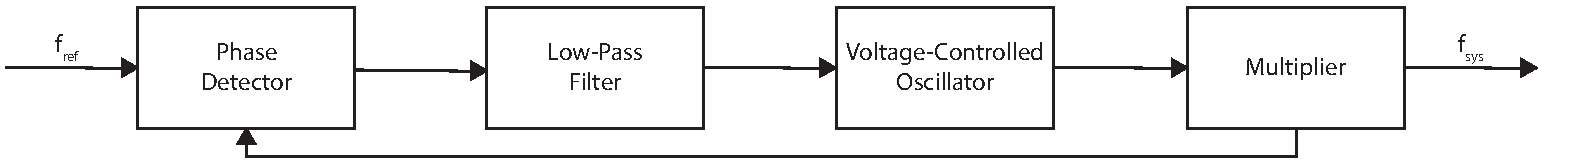
\includegraphics[width=\textwidth]
  {../figure/digital-signal-synthesis/clock-generation.pdf}
  \caption{Clock generation signal generation with \gls{pll} and multiplier.
    The phase detector compares the output system phase with the reference
    phase and yields a non-linear error response. The low-pass filter removes
    fast oscillations. The \gls{vco} changes the output phase in dependence
    of the error response. Finally system and reference phase will go in lock.
    }\label{fig:dds_clock_generation}
\end{figure}
\Cref{fig:dds_clock_generation} the system clock generation from a reference
signal is illustrated. The phase detector yields a non-linear error response
comparing the output signal phase with the reference signal phase. After a
low-pass filter removes fast oscillations a \gls{vco} changes its phase
proportional to the error signal. Finally a frequency multiplier creates
harmonics of the reference frequency and extracts a programmed frequency
multiple of $M$ such that the system frequency relates to the reference
clock by $f_\text{sys}=Mf_\text{ref}$ with $1<M\in\mathbb{N}$.

\subsection{Parameter modulation}

So far we only discussed the case of frequency modulation. We will see that
the previous architecture can be easily extended to support amplitude
and phase modulation too.
\begin{figure}[htb]
  \centering
  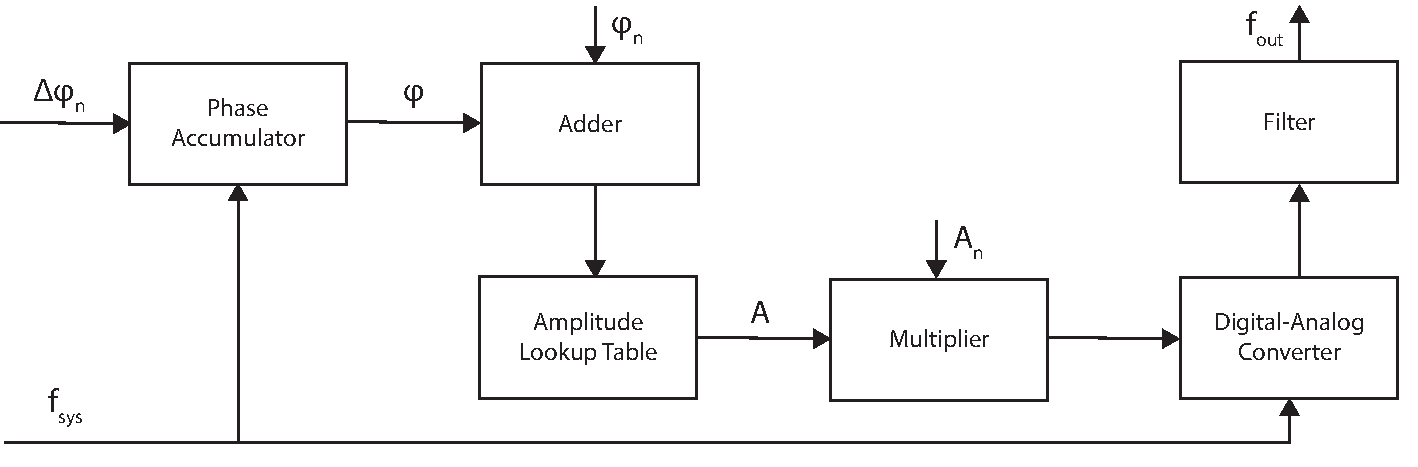
\includegraphics[width=\textwidth]
  {../figure/digital-signal-synthesis/modulation-architecture.pdf}
  \caption{\gls{dds} architecture supporting modulation of frequency,
    amplitude and phase offset parameters. Phase accumulator increment is now
    time dependent. The phase offset is also time dependent is added as last
    step to the phase accumulator before supplied to the \gls{dac}. The time
    dependent amplitude parameter is multiplied with the amplitude obtained
    from the lookup table.
    }\label{fig:dds_modulation_architecture}
\end{figure}
In \Cref{fig:dds_modulation_architecture} we can see one realization of an
architecture that supports amplitude, frequency and phase modulation. The main
components are the same as in \Cref{fig:dds_simple_architecture}. In addition
we have an adder for a time dependent phase offset and a multiplier for the
digital amplitude value obtained from the lookup table. The time dependence
of the parameters can be either determined by reading from memory or through
generation of another circuit. In a later section we will discuss the case of
a linear frequency sweep provided by a digital ramp.

\section{Quantization effects}

At the beginning of this chapter we elaborated greatly on the advantages that
digital signal synthesis has to offer. Yet we know that every technical design
involves its unqiue set of compromises. One important part in any engineering
process is to carefully evaluate the implications of these compromises. In
that sense we will discuss the side-effects arising from the digital nature of
digital signal synthesis and what methods there exists to reduce them.

\subsubsection{Phase jitter}

Phase jitter is created when one configures an output frequency for which
$\Delta\varphi$ is not a divider of $2^N$. In this case a phase error of
$-\varphi/(\Delta\varphi)$ builds up until it reaches a full clock period. One
method to circumvent the phase error is to add a delay line after the phase
accumulator\cite{Vankka2013}.

\subsubsection{Phase truncation}

Phase truncation occurs because the amplitude lookup table usually has a
reduced precision $P$ compared to the phase accumulator. The reduced precision
is necessary as most phase accumulators in \gls{dds} nowadays have at least 
$N=\SI{32}{\bit}$ entries and a lookup table supporting that many entries at
high frequencies becomes impractical~\cite{Cordesses2004}. Fortunately there
are many procedures to use the limited memory of a sinewave lookup table
more efficiently. For example one can reduce the sinewave data to the domain
from $0$ to $\pi/4$ and use symmetry to infer the values from $\pi/4$ to
$2\pi$. Sophisticated compressions methods allow compression ratios up to
165:1~\cite{Cordesses2004} so that in practice phase truncation is not a
problem.

There of course exists many more sources of signal imperfection from which
many can be described analytically~\cite{Goldberg1994}. 

\section{Frequency response}

In the previous section we discussed how the signal amplitude deviates from
the ideal amplitude because of reduced precision. In addition the theory of
digital signal synthesis describes a sinc dependency of the amplitude with
respect to frequency caused by the finite precision of the \gls{dac}. The
sinc response can be easily modulated by the zero-order hold model used
in signal processing. The zero-order hold model assumes that a signal $x(t)$
is reconstructed by a piecewise linear approximation
\begin{equation}
  x(t)
  \approx
  \sum_{n\in\mathbb{Z}}x_n\theta\left(\frac{t}{T}-\frac{1-2n}{2}\right),
\end{equation}
where $\theta(t)$ denotes the Heaviside function.

\section{Frequency resolution}

We apply a reference signal of
\begin{equation}
  f_\text{ref}=\SI{10}{\mega\hertz}
\end{equation}
configured to be used with a \gls{pll} multiplier of
$N=100$ yielding a system clock of
\begin{equation}
  f_\text{sys}=Nf_\text{ref}=\SI{1}{\giga\hertz}.
\end{equation}
The timer clock used for the linear ramp and memory playback runs with
a quarter of the system clock
\begin{equation}
  f_\text{timer}=f_\text{sys}/4=\SI{250}{\mega\hertz}.
\end{equation}

The \gls{ad9910} uses a \SI{14}{\bit} \gls{asf} and \SI{32}{\bit} \gls{ftw}
to parameterize amplitude $A(t)$ and output frequency $f(t)$ by
\begin{align}
  FTW
  :=
  \left\lfloor2^{32}\left(\frac{f_\text{out}}{f_\text{sys}}\right)\right\rceil
  &&
  ASF
  :=
  \left\lfloor\frac{A_\text{out}}{2^{14}}\right\rceil
  \label{eq:elec:ftwasf}
\end{align}
wherein $\lfloor{\cdot}\rceil$ rounds the given float to the nearest integer.
The theoretical limit for the maximum output frequency then is found via
\begin{equation*}
  f_\text{max}
  =
  \left(1-\frac{2^{31}-1}{2^{32}}\right)f_\text{sys}
  =
  \left(\frac{1}{2}-\frac{1}{2^{31}}\right)f_\text{sys}
  \approx
  \frac{1}{2}f_\text{sys}
  =
  \SI{500}{\mega\hertz}.
\end{equation*}
Yet the datasheet~\cite{AD9910} reports $f_\text{max}=\SI{420}{\mega\hertz}$
and in fact we found the output signal to be very noisy at the theoretical
limit.

We continue with the assessment of the digital ramp that does a unidrectional
linear sweep on the frequency from \SI{90}{\mega\hertz} to
\SI{110}{\mega\hertz}. The digital ramp of the \gls{ad9910} lets us define
a \gls{ftw} step $M$ word of \SI{32}{\bit} as well as a step rate word $S$ of
\SI{16}{\bit} resolution. They relate to the frequency step and the time
step through
\begin{align}
  \Delta f
  =
  \frac{M}{2^{32}}f_\text{sys}
  &&
  \Delta t
  =
  \frac{S}{f_\text{timer}}
  =
  \frac{S}{4f_\text{sys}}.
  \label{eq:elec:step}
\end{align}
The sweep duration is deterimened by $S,M$ through
\begin{equation}
  T_\text{duration}
  =
  \frac{f_\text{upper}-f_\text{lower}}{\Delta f}\Delta t
  =
  2^{32}\frac{f_\text{upper}-f_\text{lower}}
  {f_\text{sys}}\frac{S/M}{f_\text{timer}}
\end{equation}
for a target sweep duration of $T_\text{duration}=\SI{10}{ms}$ we find
\begin{equation*}
  \frac{S}{M}
  =
  \frac{T f_\text{timer}}{2^{32}}
  \frac{f_\text{sys}}{f_\text{upper}-f_\text{lower}}
  =
  \frac{10^9}{2^{35}}
  \approx
  \num{2.9104e-2}
  =
  \frac{1819}{62500}
\end{equation*}
the last step can be obtained by best ratio approximation using continued
fractions as for example described in~\cite{Ashley2003}. It should be kept in
mind that the best ratio approximation is likable to introduce an error,
therefore realistic durations may differ from the configured value and it
is possible that better approximations exist that allow smaller $\Delta f,
\Delta t$, thus providing a sweep resolution. In the above case the given
time duration translates to
\begin{align*}
  \Delta f
  =
  \frac{62500}{2^{32}}f_\text{sys}
  \approx
  \SI{145}{\kilo\hertz}
  &&
  \Delta t
  =
  \frac{1819}{f_\text{timer}}
  \approx
  \SI{7.28}{\micro\second}
\end{align*}
or $(f_\text{upper}-f_\text{lower})/\Delta f=138$ discrete data points.

Eventually we are left with the assessment of the amplitude sequence. The
memory fits at most 1024 discrete amplitude values and the \gls{ad9910}
allows us to set the time spent at each amplitude value via the \SI{16}{\bit}
playback rate $P$ word
\begin{equation}
  \Delta t
  =
  \frac{P}{f_\text{timer}}
  =
  \frac{4P}{f_\text{sys}}
\end{equation}
which gives us range from $\min\Delta t=\SI{4}{\nano\second}$ to
$\max\Delta t=\SI{26.14}{\micro\second}$. As we incorporate all of the 1024
data points this gives us a duration range from about
$\min T=\SI{4}{\micro\second}$ to $\max T=\SI{26.84}{\milli\second}$.
